\chapter{Badania eksperymentalne}\label{chapt:testsResults}
W tym rozdziale przeanalizowano wyniki eksperymentów przeprowadzonych na zbiorach danych \textbf{BuzzFeed}, \textbf{ISOT} oraz \textbf{WELFake}, stosując trzy tryby podziału danych: \textbf{klasyczny}, \textbf{few-shot} i \textbf{one-shot}. Oceniono skuteczność modeli za pomocą metryk, takich jak \textbf{dokładność}, \textbf{miara F1}, \textbf{czas wykonania} oraz \textbf{obszar pod krzywą ROC}. Uwzględniono również czas realizacji i stabilność modeli, wykorzystując podział na osadzenia z \textbf{BERT}, \textbf{RoBERTa} i \textbf{SBERT}. Wyniki zobrazowano wykresami słupkowymi w przypadku \textbf{dokładności} i \textbf{miary F1} oraz tabelami wynikowymi dla \textbf{miary F1}, \textbf{czasu wykonania} oraz \textbf{testów statystycznych}. Dodatkowo, wszystkie inne wykresy porównawcze dla pozostałych metryk zostały umieszczone w \textbf{dodatku}. Pozwoliło to skupić się na najważniejszych wybranych metrykach, oceniając skuteczność \textbf{metody17}, \textbf{metody18}, \textbf{metody19} i \textbf{metody20} w zależności od specyfiki danych i strategii uczenia. Dalsza część rozdziału szczegółowo omawia rezultaty dla każdego zbioru danych, uwzględniając ich charakterystykę i wpływ trybu podziału na wyniki.

W każdym podrozdziale niniejszego rozdziału wyniki pogrupowano według analizowanych zbiorów danych (\textbf{BuzzFeed}, \textbf{ISOT}, \textbf{WELFake}) oraz technik uczenia stosowanych w różnych kontekstach podziału danych.

Przykładowo, diagramy opisujące \textbf{dokładność} i \textbf{miarę F1} podzielono na trzy części:
\begin{itemize}
	\item górna część prezentuje wyniki z wykorzystaniem osadzeń \textbf{BERT},
	\item środkowa przedstawia dane z osadzeniami \textbf{RoBERTa},
	\item dolna dotyczy trybu osadzeń \textbf{SBERT}.
\end{itemize}

Taka organizacja wyników umożliwia szczegółowe przeanalizowanie wpływu różnych trybów podziału danych na skuteczność metod. Natomiast tabele z wynikami dla \textbf{czasu wykonania} oraz \textbf{obszar pod krzywą ROC} będą zawierały kolumnę \textbf{Metoda}, która obejmuje nazwy metod, i kolejne kolumny reprezentujące wyniki dla każdego rodzaju osadzeń, w naszym przypadku \textbf{BERT}, \textbf{RoBERTa} i \textbf{SBERT}. Omówienie wszystkich wyników zostało przeprowadzone z klasyfikacją algorytmów według stosowanych podejść i architektury. W trakcie opisu analizy wyników użyłem \textbf{few-shot} zamiast \textbf{uczenia jednokrotnego} oraz \textbf{one-shot} zamiast \textbf{uczenia na kilku przykładach}, co będzie bardziej jasnym przy przeglądzie wykresów oraz tabelek z danymi. Dane zaokrąglono do dwóch miejsc po przecinku.

\section{Analiza wyników dla datasetu \textbf{BuzzFeed}}
\label{subsec:buzzfeed_analysis}

W tej sekcji przedstawiono wyniki dla datasetu \textbf{BuzzFeed} w trybach: \textbf{klasycznym}, \textbf{few-shot} oraz \textbf{one-shot}. Analiza obejmuje kluczowe metryki (Accuracy, F1-Score, ROC-AUC) dla embeddingów BERT, RoBERTa i SBERT, zwięźle omówione w kontekście wykresów. Dla metod autorskich (\texttt{Metoda17}--\texttt{Metoda20}) podano przyczyny wyników. Wnioski zebrano w sekcji podsumowującej.

\subsection{Wyniki w trybie klasycznym}

\subsubsection{Accuracy}
Wykresy Accuracy (\ref{fig:buzzfeed_classic_accuracy}) pokazują, że dla BERT \texttt{Metoda12-catboost}, \texttt{Metoda12-rf} i \texttt{Metoda19} osiągnęły ~0.6, a \texttt{Metoda18} najniższe (~0.38). Dla RoBERTa \texttt{Metoda10} i \texttt{Metoda12-catboost} osiągnęły ~0.68, a \texttt{Metoda1-2}, \texttt{Metoda17}, \texttt{Metoda19} ~0.49. Dla SBERT \texttt{Metoda13} i \texttt{Metoda12-catboost} miały ~0.73, a \texttt{Metoda1-3}, \texttt{Metoda3}, \texttt{Metoda4} ~0.49. \texttt{Metoda17} (VotingClassifier) zawodzi dla RoBERTa z powodu niedopasowania hiperparametrów, \texttt{Metoda18} (stacking) jest słaba dla BERT z powodu prostej architektury, \texttt{Metoda19} (stacking) osiąga wysokie wyniki dla BERT/SBERT dzięki zoptymalizowanemu łączeniu modeli, a \texttt{Metoda20} jest średnia z powodu braku balansowania klas.

\begin{figure}[H]
	\centering
	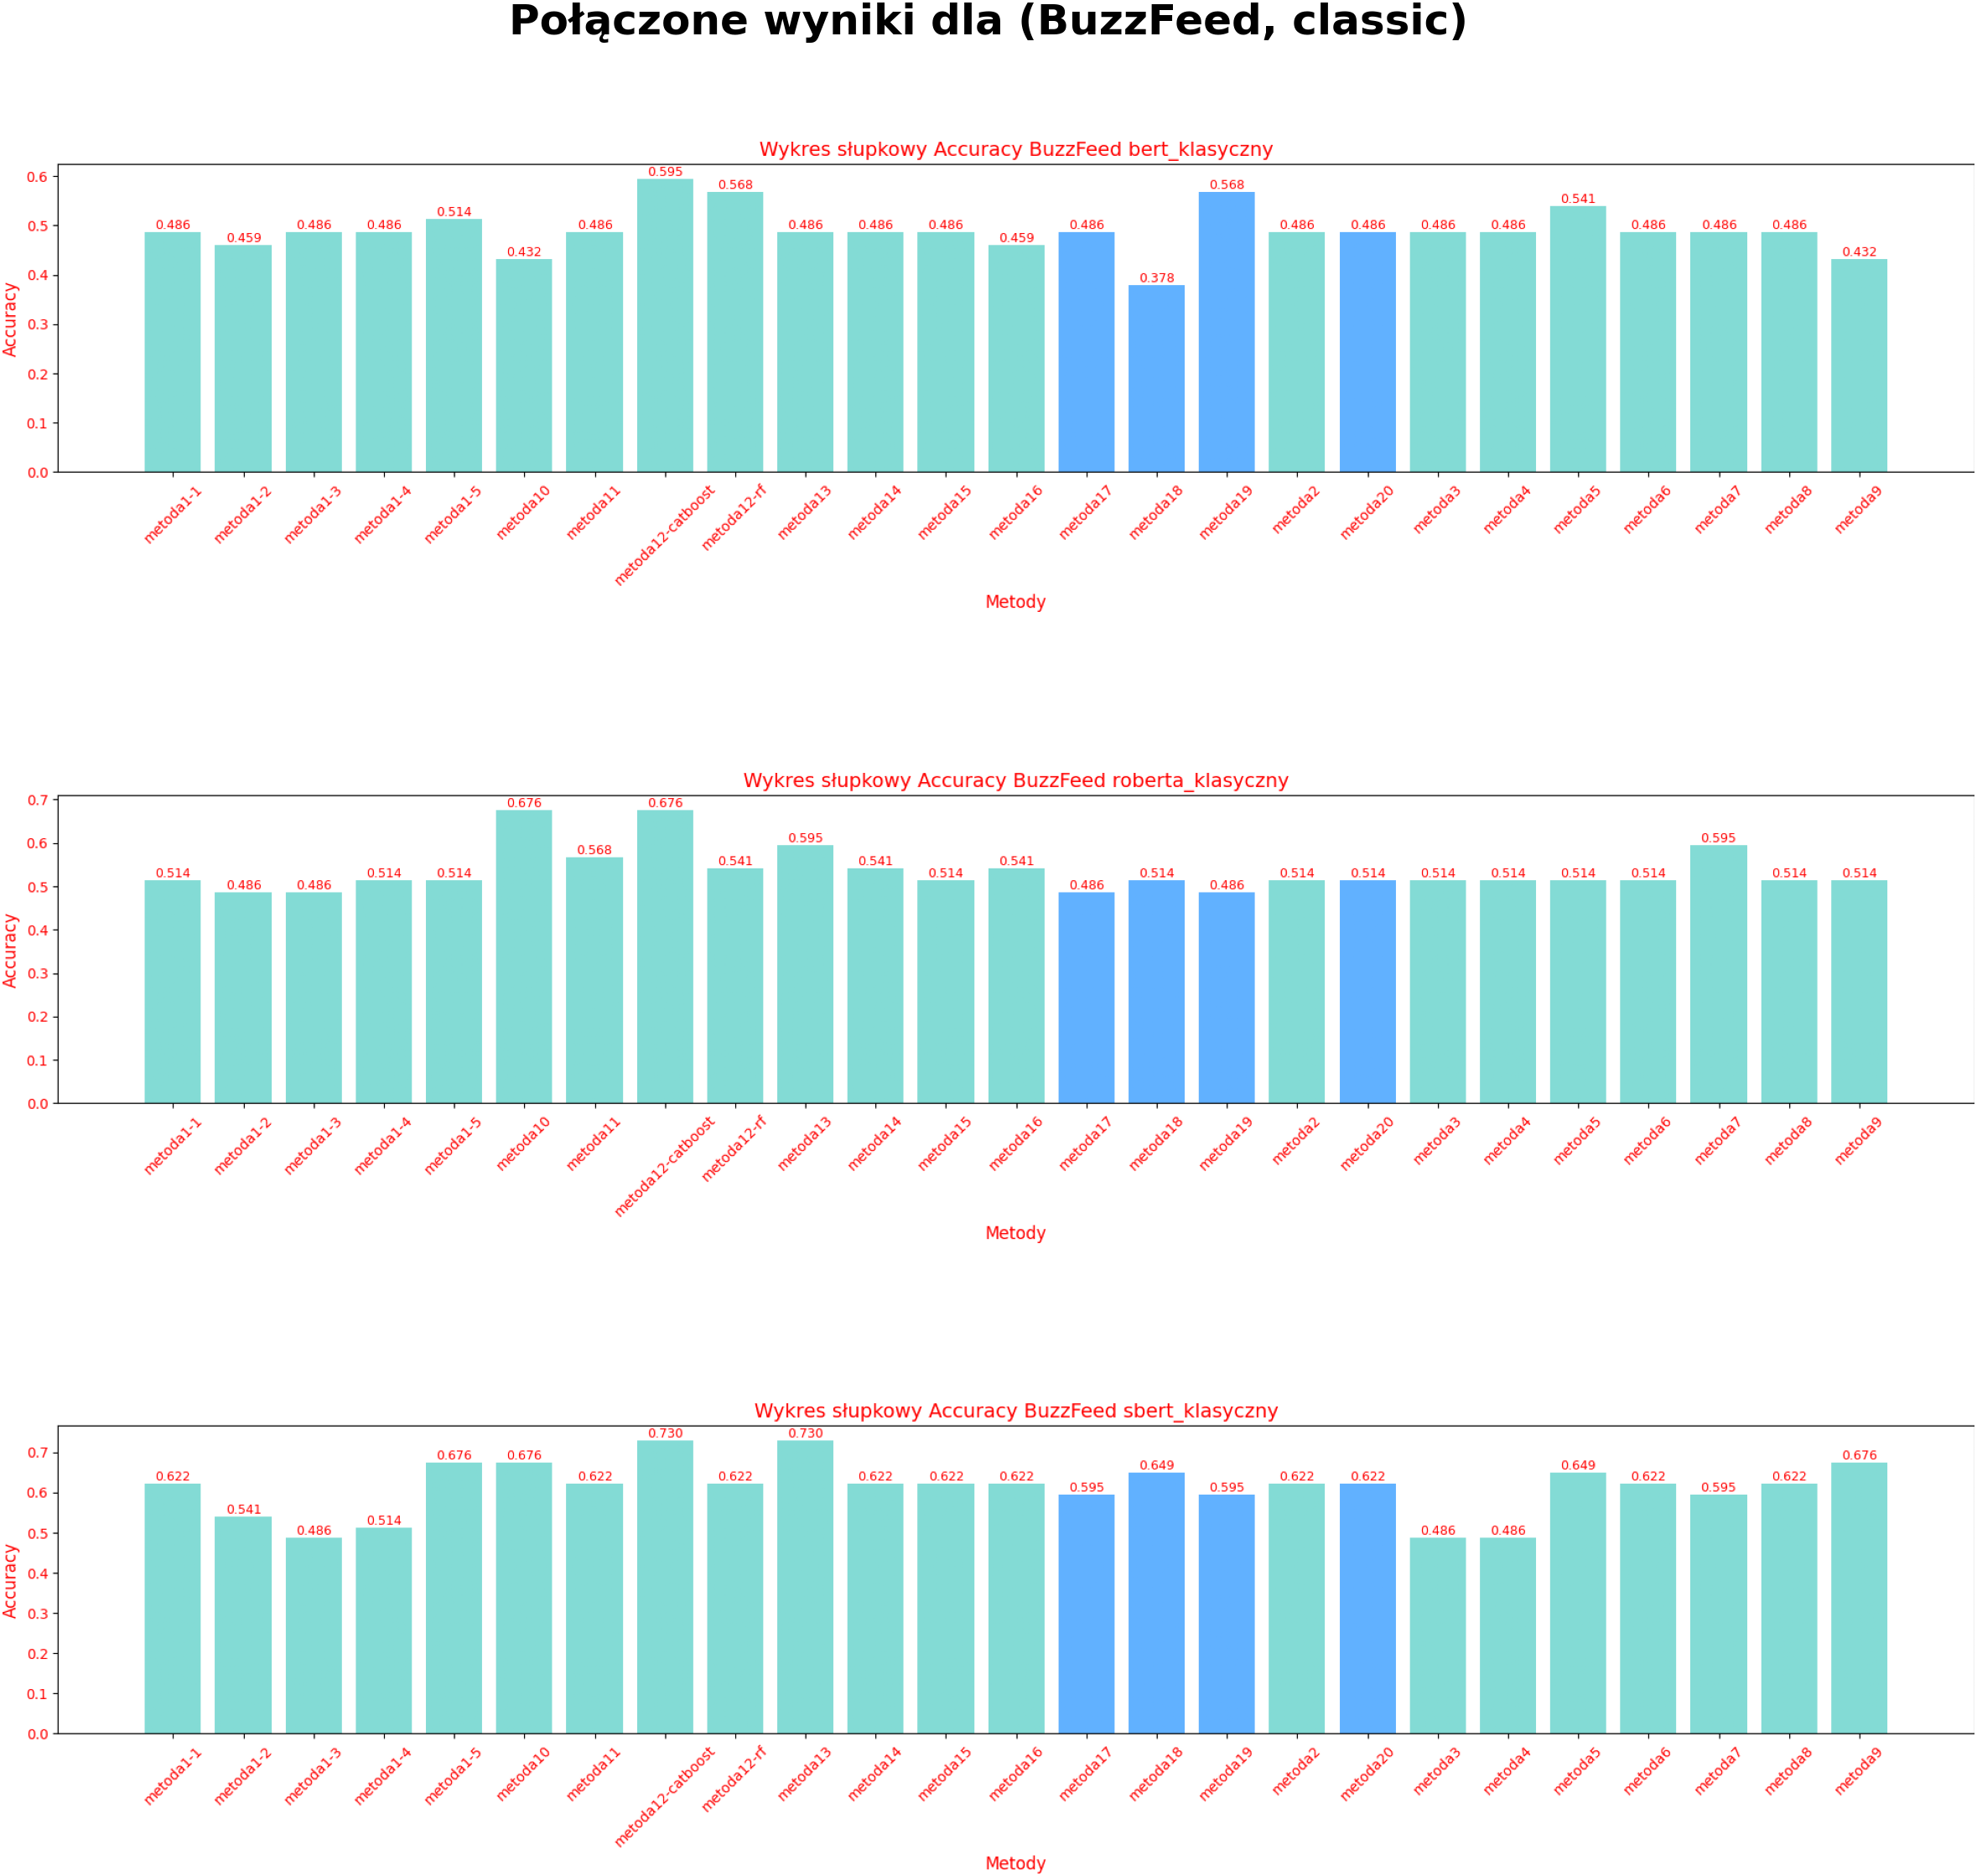
\includegraphics[width=0.99\textwidth]{img/stats/BuzzFeed_classic/BuzzFeed_classic_Combined_Accuracy_bar_chart.png}
	\caption{Histogram rozkładu \textbf{Dokładności (Accuracy)}.}
	\label{fig:buzzfeed_classic_accuracy}
\end{figure}

\subsubsection{F1-Score}
Wykresy F1-Score (\ref{fig:buzzfeed_classic_f1}) wskazują, że dla BERT \texttt{Metoda19}, \texttt{Metoda17}, \texttt{Metoda12-catboost} osiągnęły najwyższe wartości, a \texttt{Metoda1-2}, \texttt{Metoda1-5} najniższe. Dla RoBERTa \texttt{Metoda1-2}, \texttt{Metoda10}, \texttt{Metoda17} były najlepsze, a \texttt{Metoda1-1}, \texttt{Metoda1-4} najgorsze. Dla SBERT \texttt{Metoda13}, \texttt{Metoda12-catboost}, \texttt{Metoda18}, \texttt{Metoda19} osiągnęły wysokie wyniki, a \texttt{Metoda1-2} najniższe. \texttt{Metoda17} osiąga wysoki F1 dla RoBERTa dzięki VotingClassifier, \texttt{Metoda18} dobrze radzi sobie dla SBERT z powodu stacking z CatBoost, \texttt{Metoda19} jest skuteczna dla BERT/SBERT dzięki modelom ensemble, a \texttt{Metoda20} średnia z powodu braku optymalizacji.

\begin{figure}[H]
	\centering
	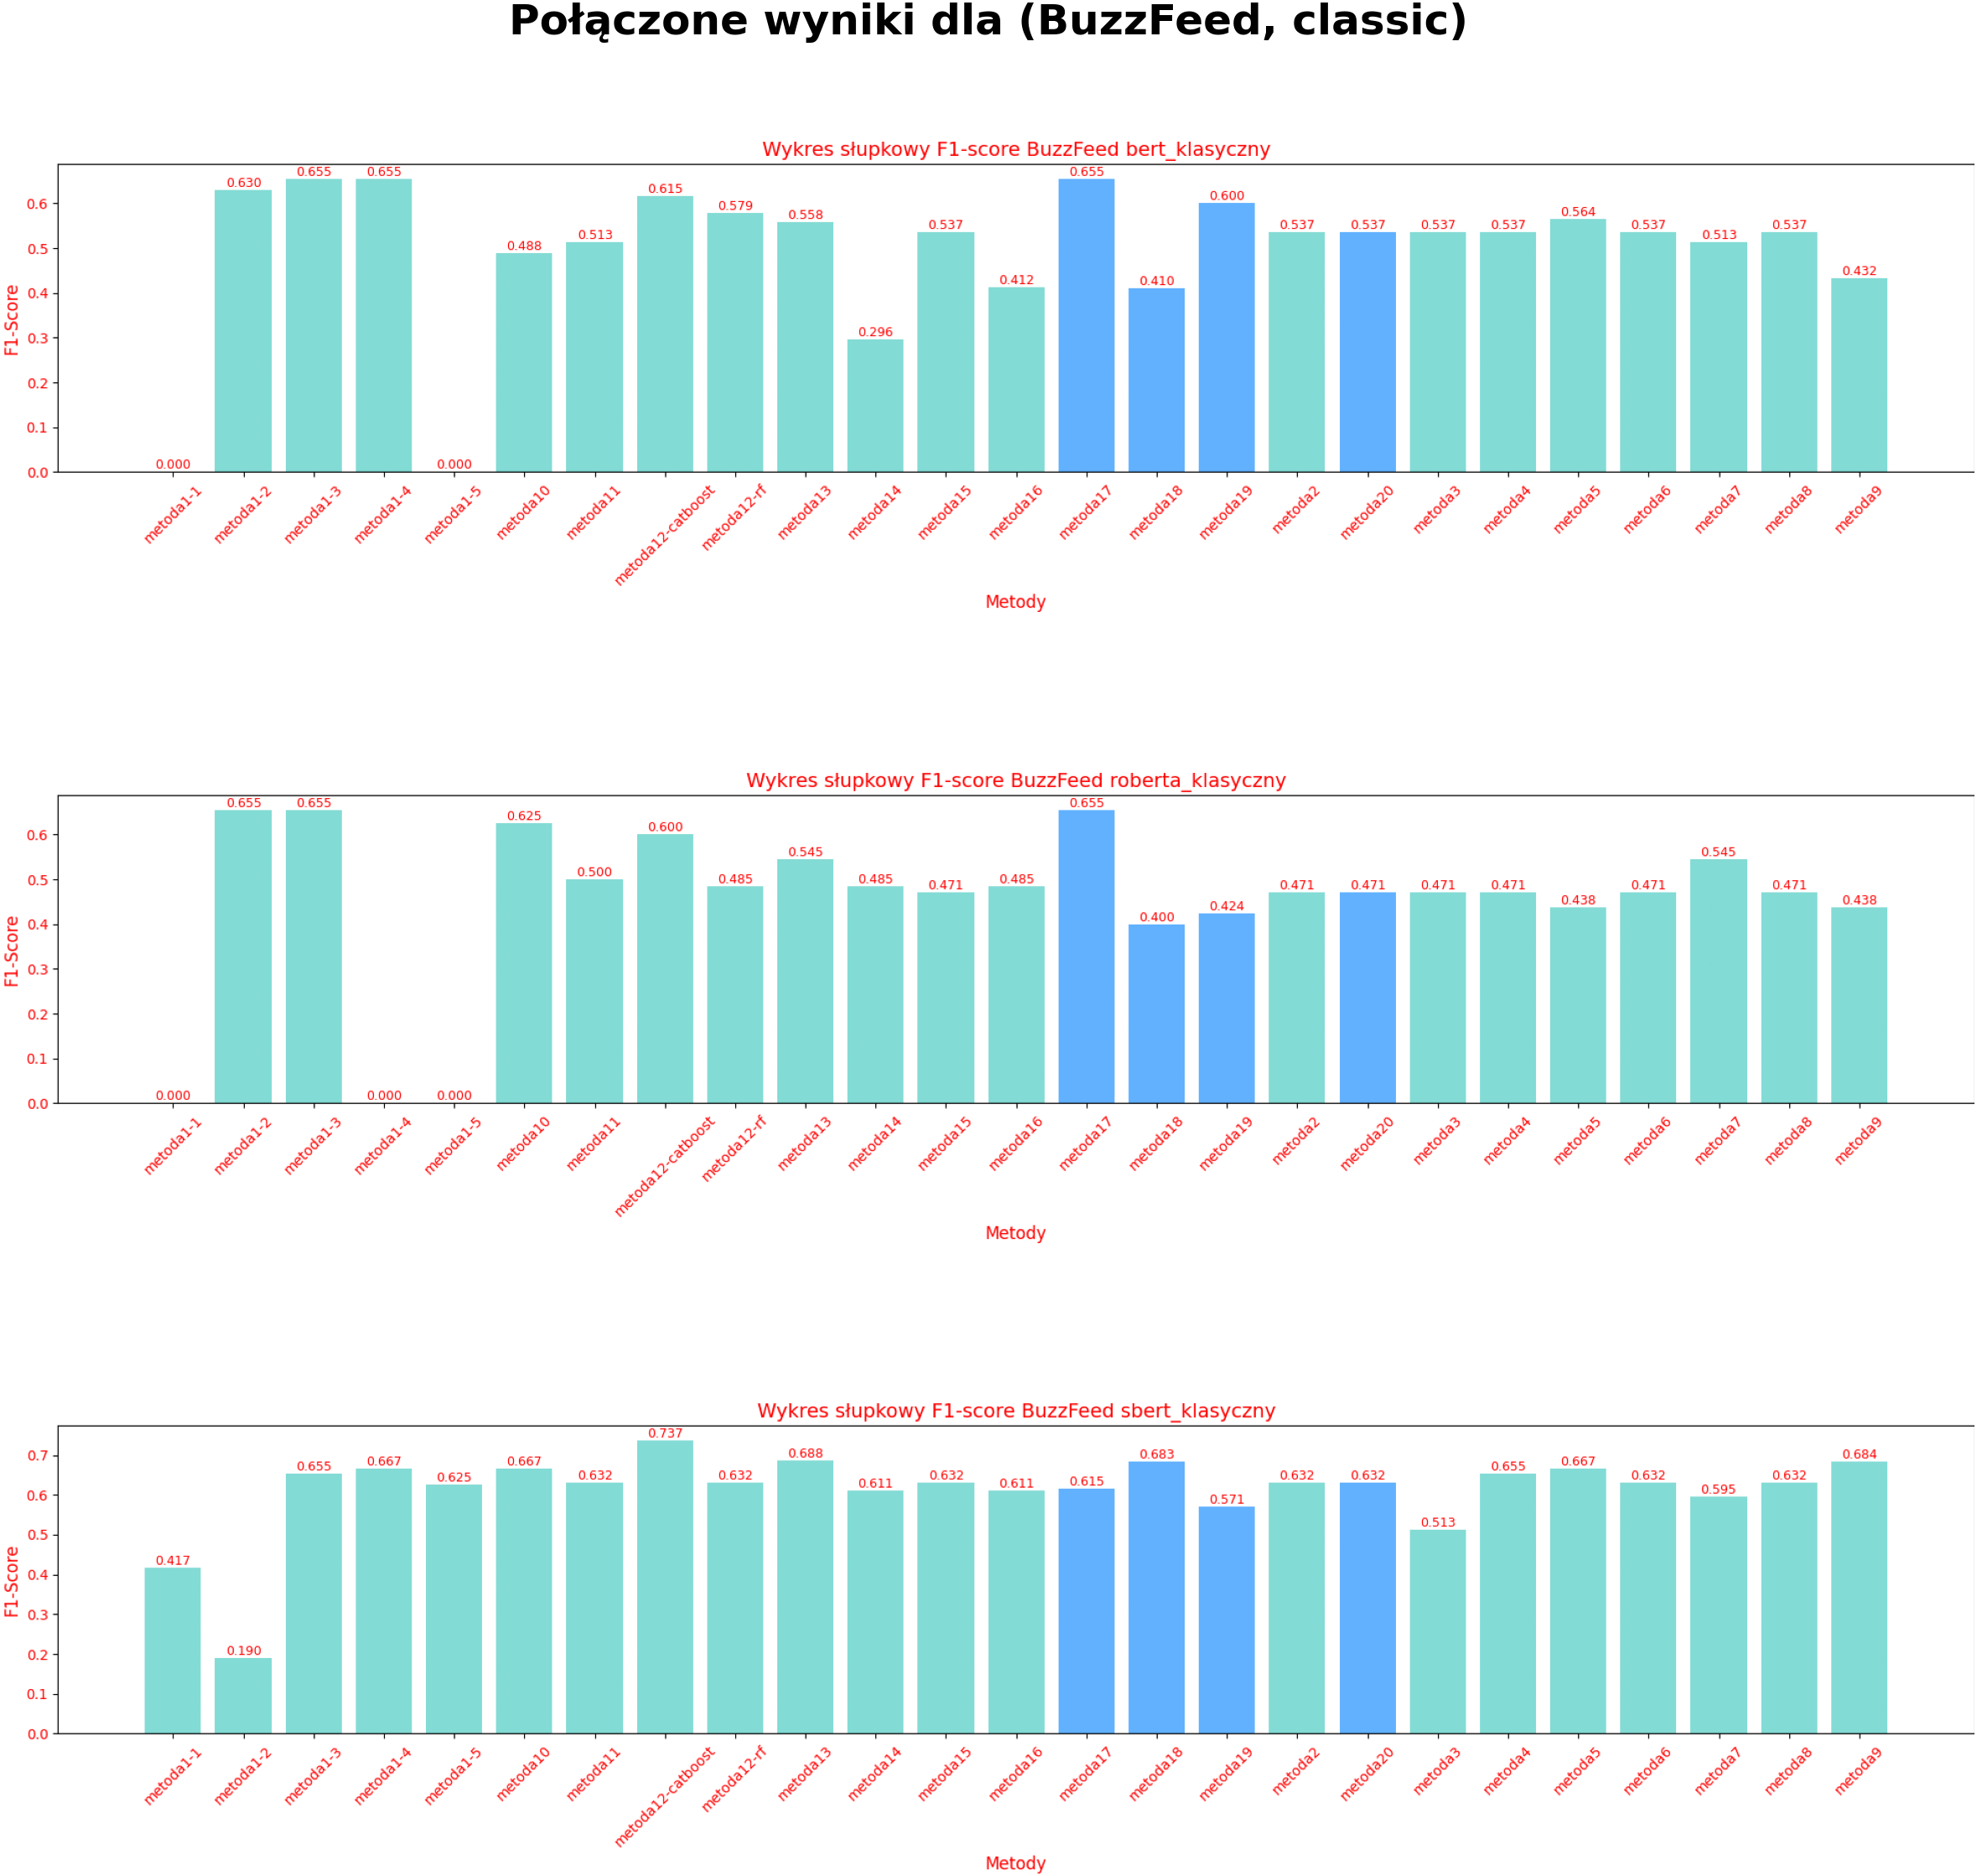
\includegraphics[width=0.99\textwidth]{img/stats/BuzzFeed_classic/BuzzFeed_classic_Combined_F1-Score_bar.png}
	\caption{Histogram rozkładu \textbf{Wyniku F1 (F1-Score)}.}
	\label{fig:buzzfeed_classic_f1}
\end{figure}

\subsubsection{ROC-AUC}
Wykresy ROC-AUC (\ref{fig:buzzfeed_classic_roc}) pokazują, że dla BERT \texttt{Metoda19} osiągnęła najwyższe wartości, a \texttt{Metoda17}, \texttt{Metoda1-4} najniższe. Dla RoBERTa \texttt{Metoda1-2}, \texttt{Metoda1-3}, \texttt{Metoda17} były najlepsze, a \texttt{Metoda14}, \texttt{Metoda19} najgorsze. Dla SBERT \texttt{Metoda1-4} osiągnęła wysoki wynik, a \texttt{Metoda4} najniższy. \texttt{Metoda17} jest skuteczna dla RoBERTa dzięki VotingClassifier, \texttt{Metoda18} słaba dla BERT z powodu prostej konfiguracji, \texttt{Metoda19} dominuje dla BERT dzięki stacking, a \texttt{Metoda20} średnia z powodu braku balansowania.

\begin{figure}[H]
	\centering
	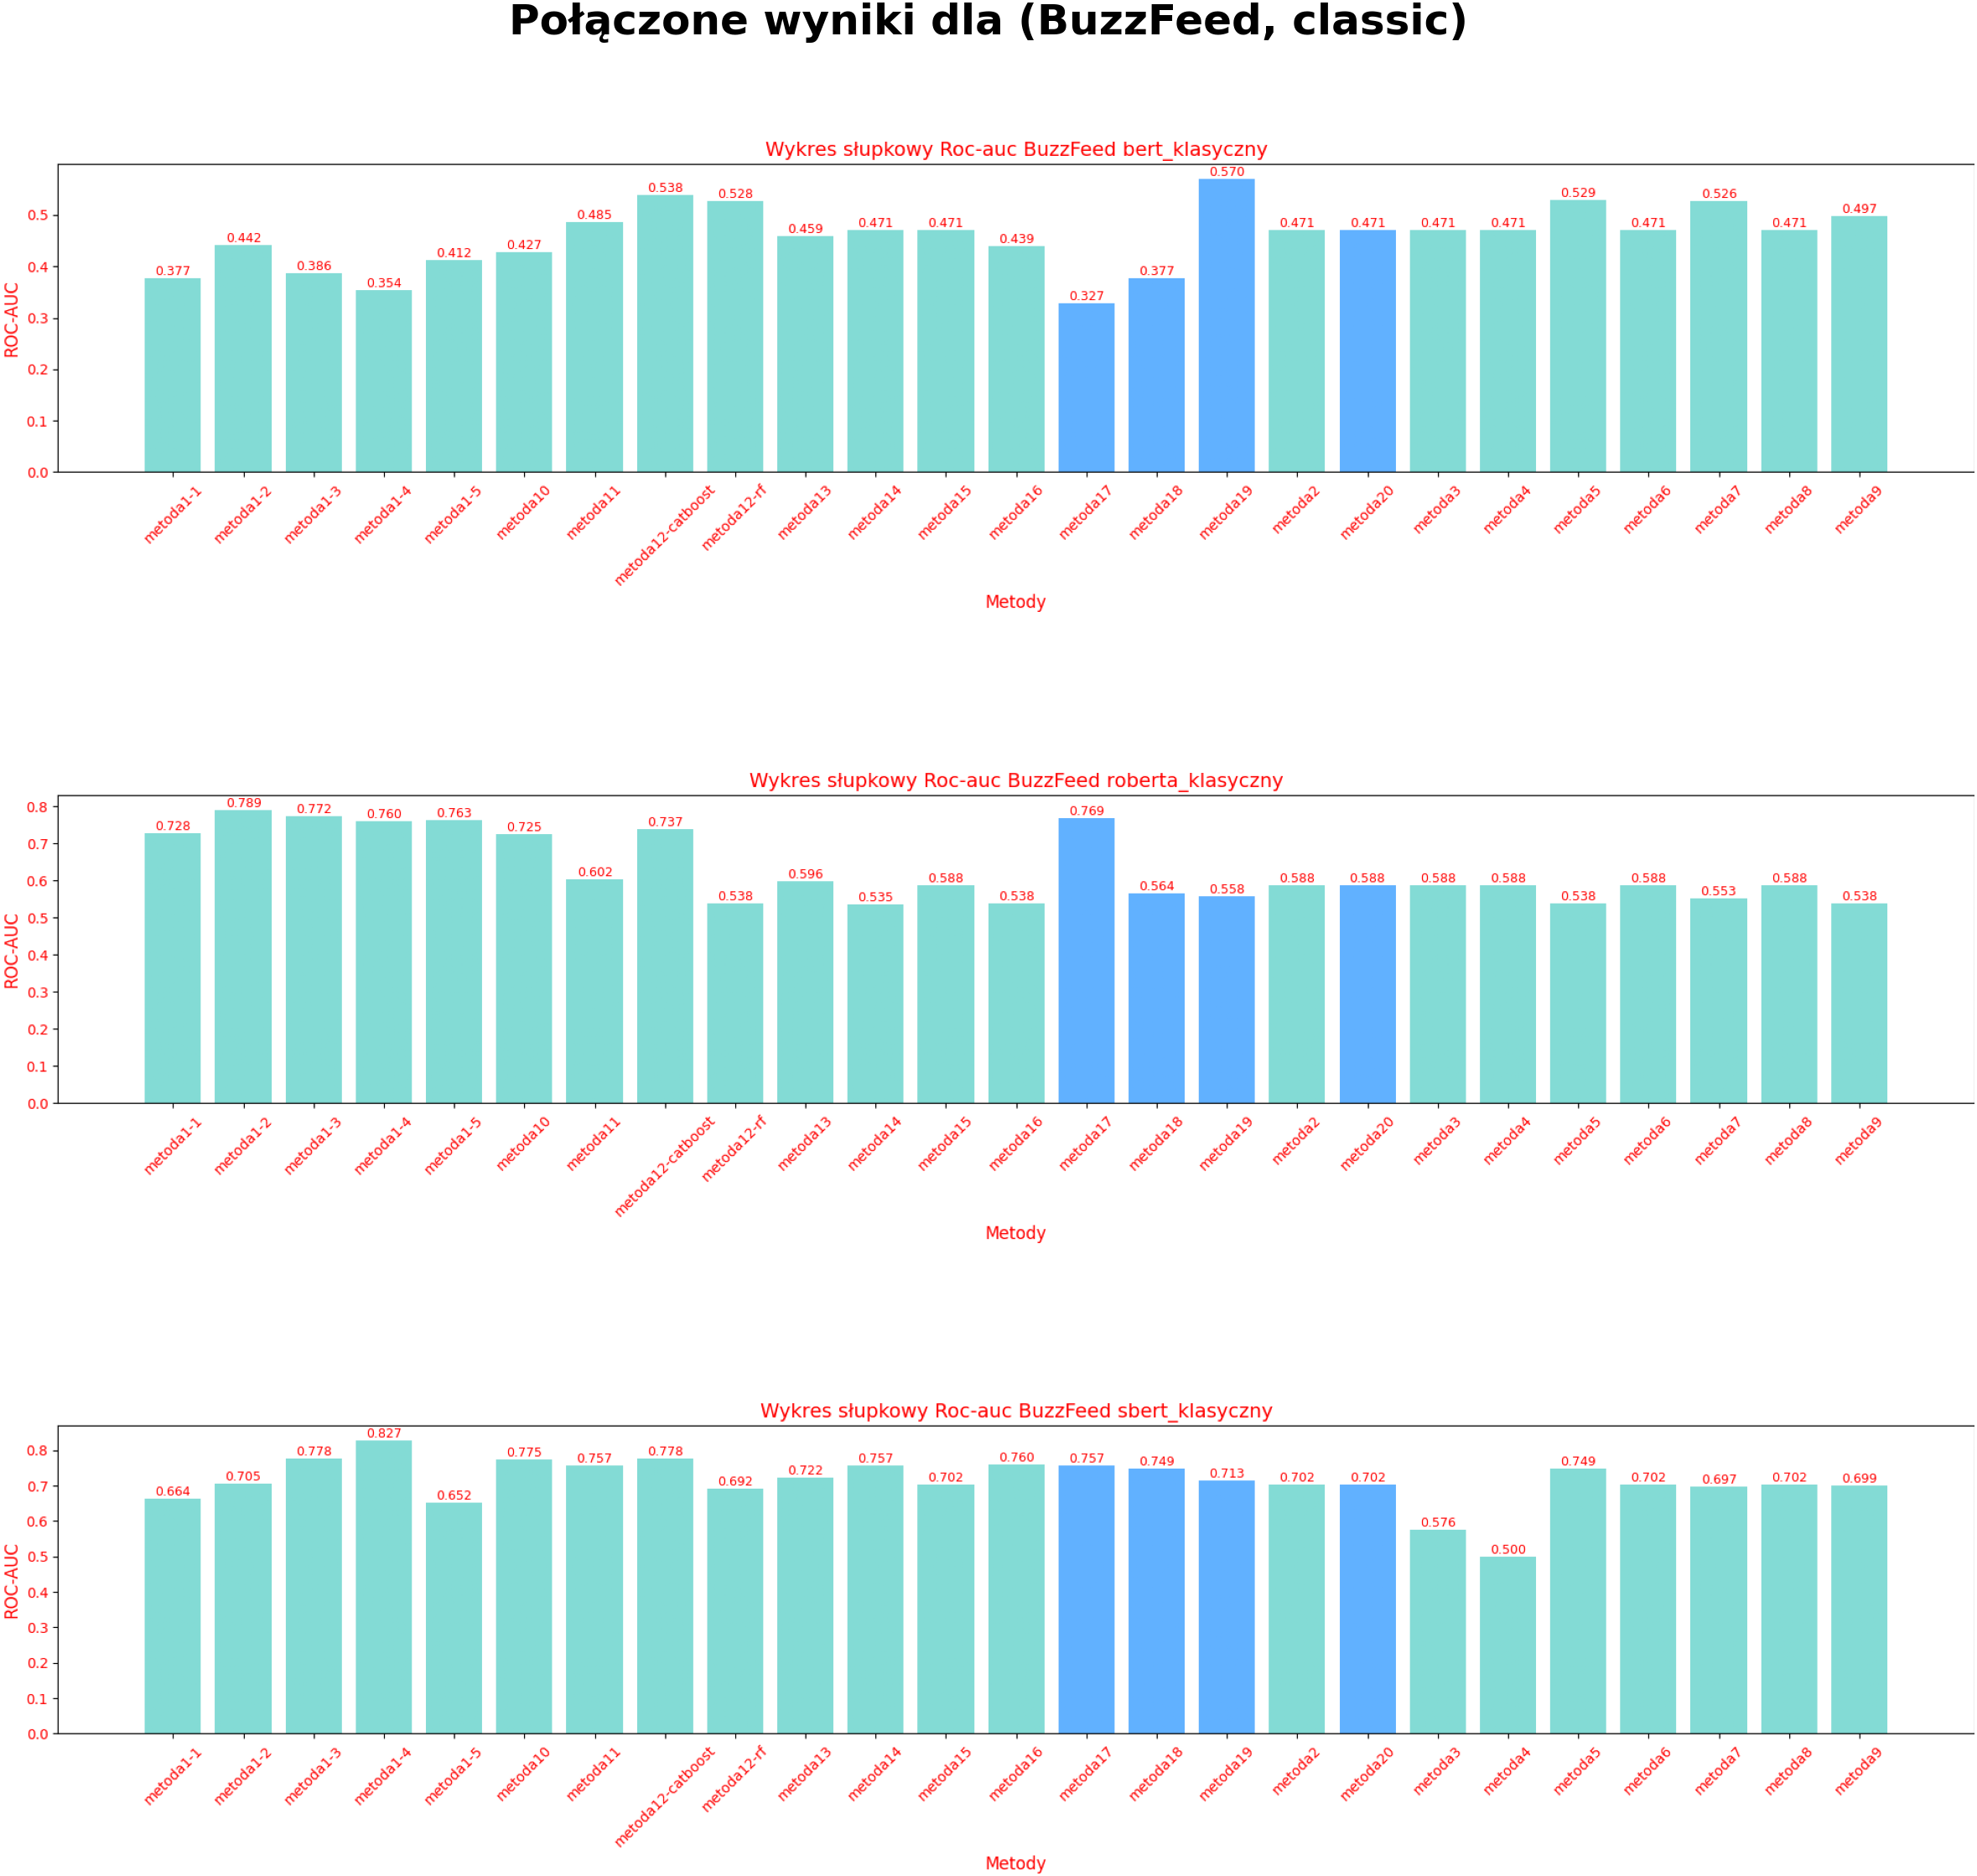
\includegraphics[width=0.99\textwidth]{img/stats/BuzzFeed_classic/BuzzFeed_classic_Combined_ROC-AUC_bar.png}
	\caption{Histogram rozkładu \textbf{Pola pod krzywą ROC-AUC (ROC-AUC)}.}
	\label{fig:buzzfeed_classic_roc}
\end{figure}

\subsection{Wyniki w trybie few-shot}

\subsubsection{Accuracy}
Wykresy Accuracy (\ref{fig:buzzfeed_few_shot_accuracy}) wskazują, że dla BERT \texttt{Metoda13}, \texttt{Metoda14}, \texttt{Metoda19} osiągnęły najlepsze wyniki, a \texttt{Metoda12-rf} najgorsze. Dla RoBERTa \texttt{Metoda18} była najlepsza, a \texttt{Metoda15}, \texttt{Metoda20} najsłabsze. Dla SBERT \texttt{Metoda19}, \texttt{Metoda5}, \texttt{Metoda13} osiągnęły ~0.7, a \texttt{Metoda12-rf} ~0.5. \texttt{Metoda17} słaba dla BERT z powodu niedopasowania VotingClassifier, \texttt{Metoda18} skuteczna dla RoBERTa dzięki stacking z CatBoost, \texttt{Metoda19} wysoka dla BERT/SBERT dzięki ensemble, \texttt{Metoda20} słaba dla RoBERTa z powodu braku optymalizacji.

\begin{figure}[H]
	\centering
	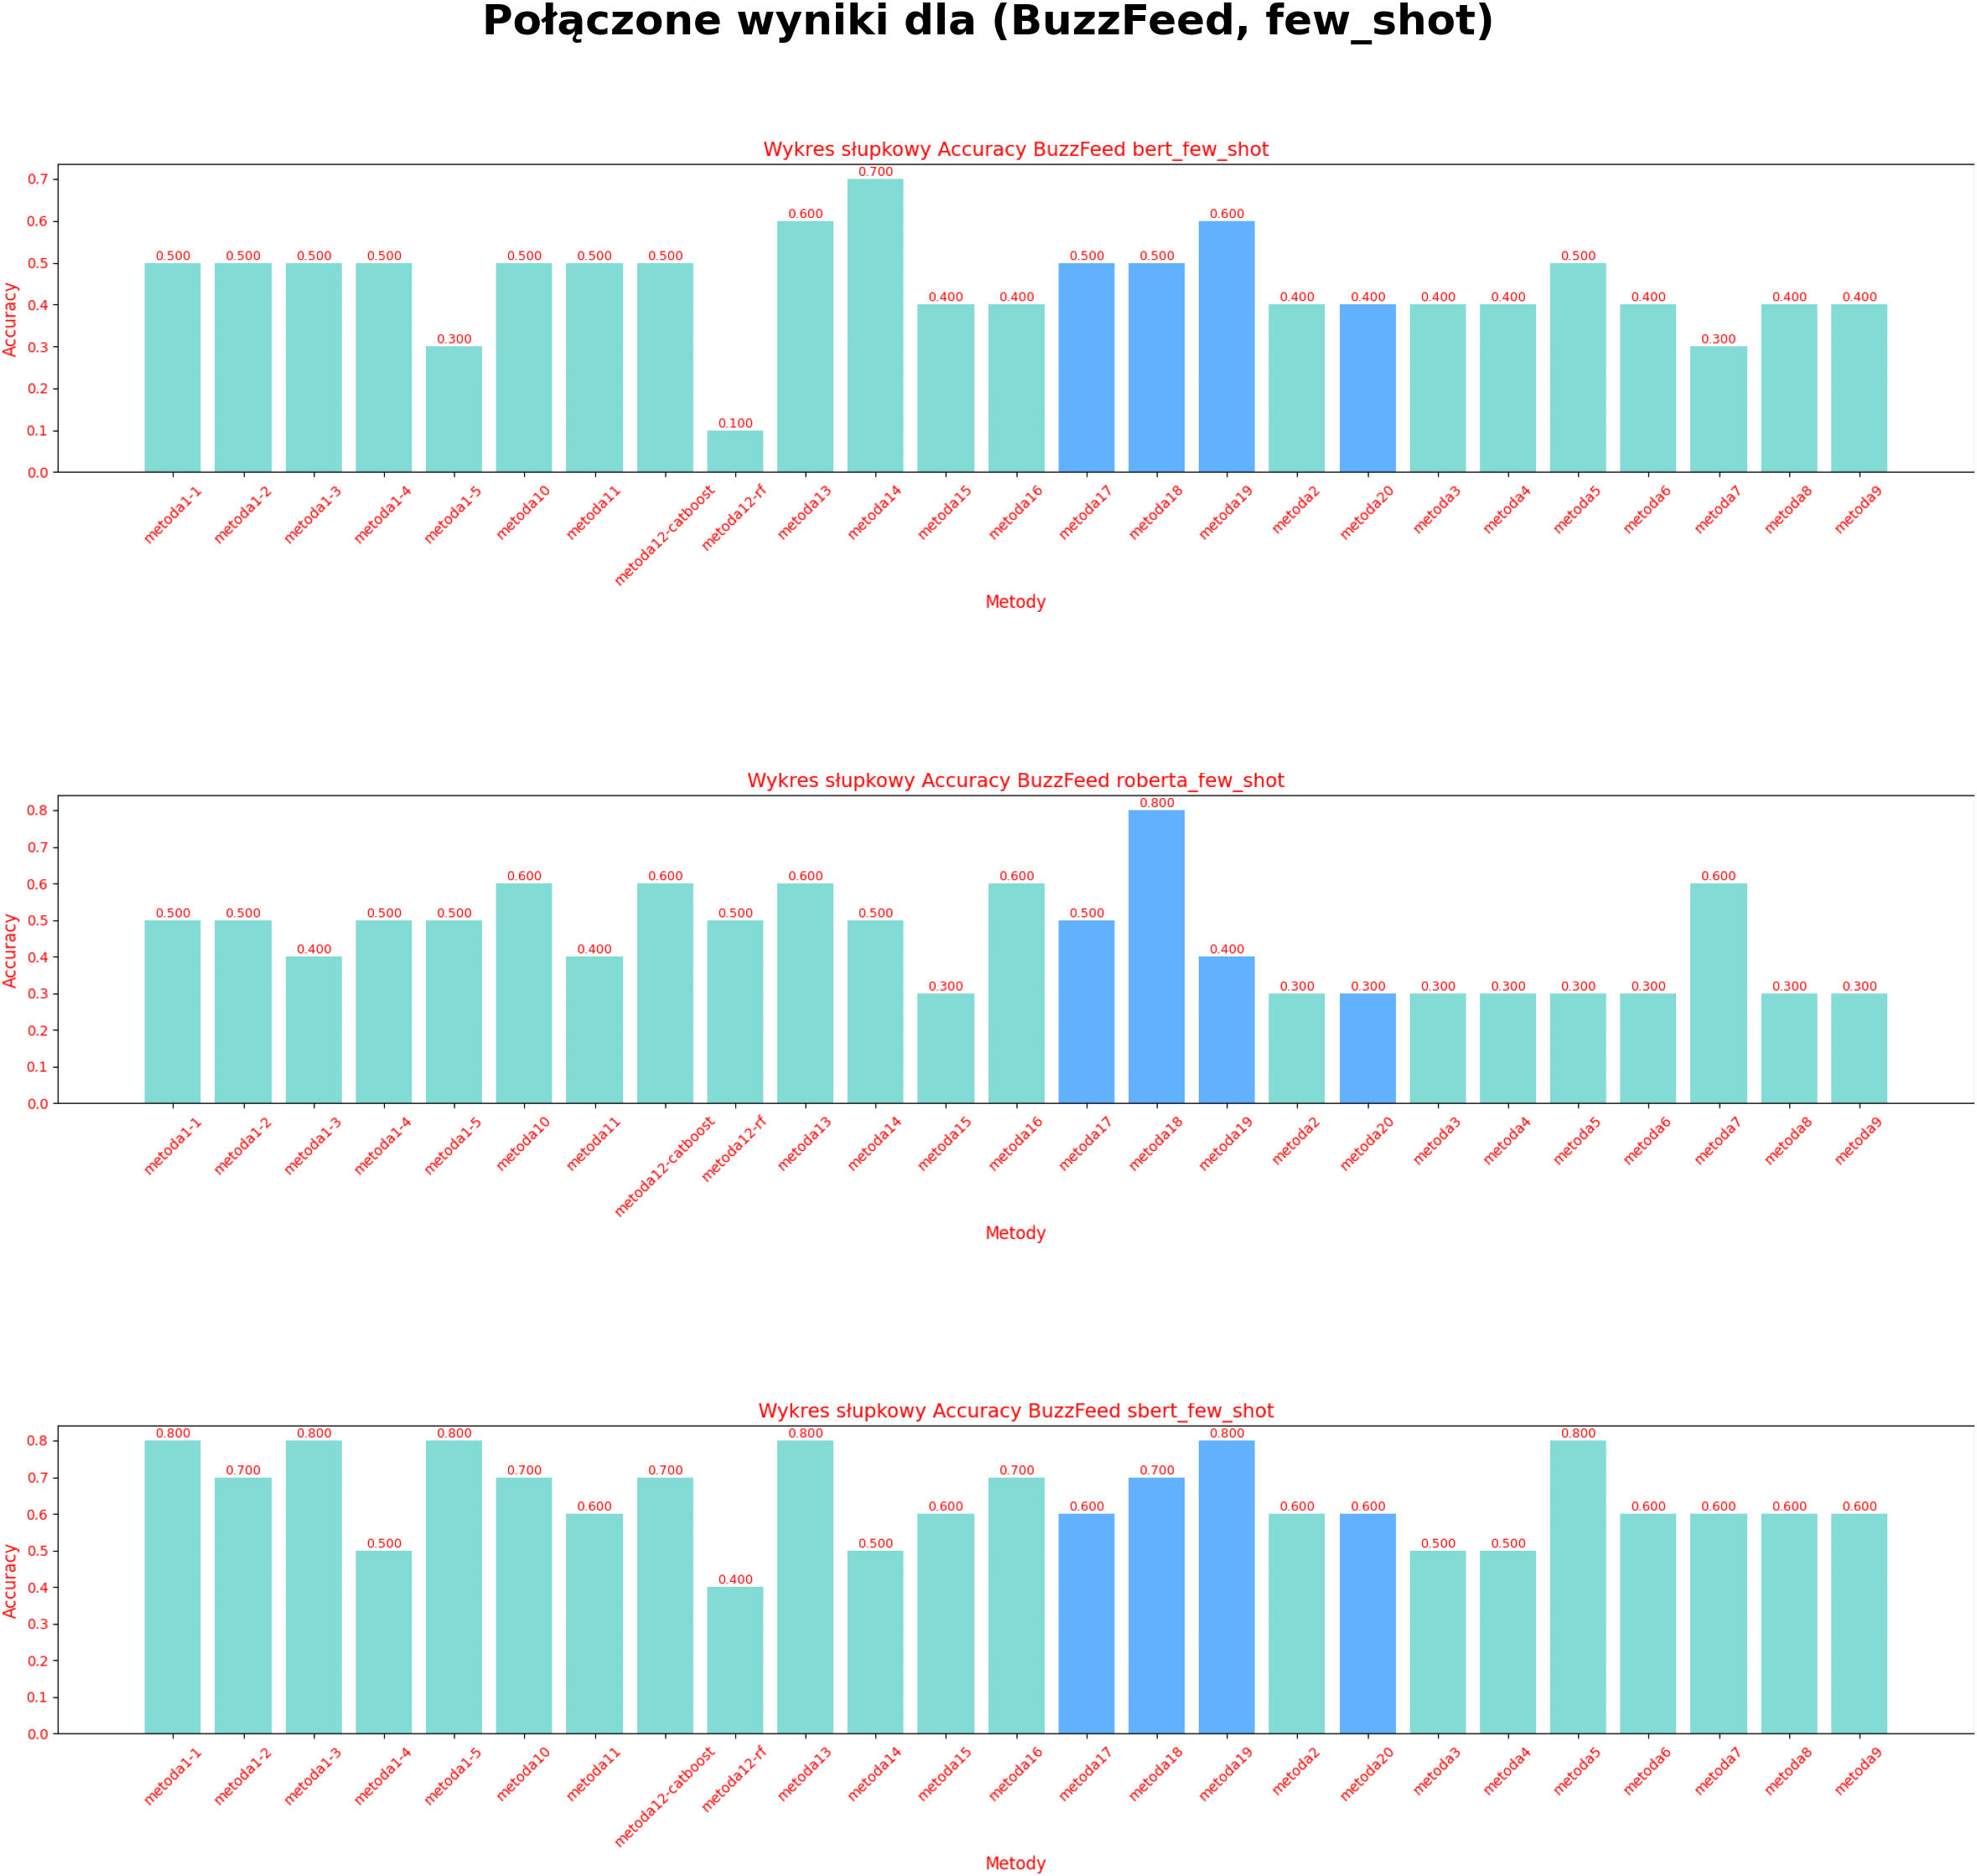
\includegraphics[width=0.99\textwidth]{img/stats/BuzzFeed_few_shot/BuzzFeed_few_shot_Combined_Accuracy_bar_chart.png}
	\caption{Histogram rozkładu \textbf{Dokładności (Accuracy)}.}
	\label{fig:buzzfeed_few_shot_accuracy}
\end{figure}

\subsubsection{F1-Score}
Wykresy F1-Score (\ref{fig:buzzfeed_few_shot_f1}) pokazują, że dla BERT \texttt{Metoda19}, \texttt{Metoda14} osiągnęły najwyższe wartości, a \texttt{Metoda17} najniższe. Dla RoBERTa \texttt{Metoda18} była najlepsza, a \texttt{Metoda20}, \texttt{Metoda17} najgorsze. Dla SBERT \texttt{Metoda13}, \texttt{Metoda19} osiągnęły wysokie wyniki, a \texttt{Metoda3} najniższe. \texttt{Metoda17} słaba dla BERT/RoBERTa z powodu VotingClassifier, \texttt{Metoda18} skuteczna dla RoBERTa dzięki stacking, \texttt{Metoda19} wysoka dla BERT/SBERT dzięki ensemble, \texttt{Metoda20} słaba dla RoBERTa z braku balansowania.

\begin{figure}[H]
	\centering
	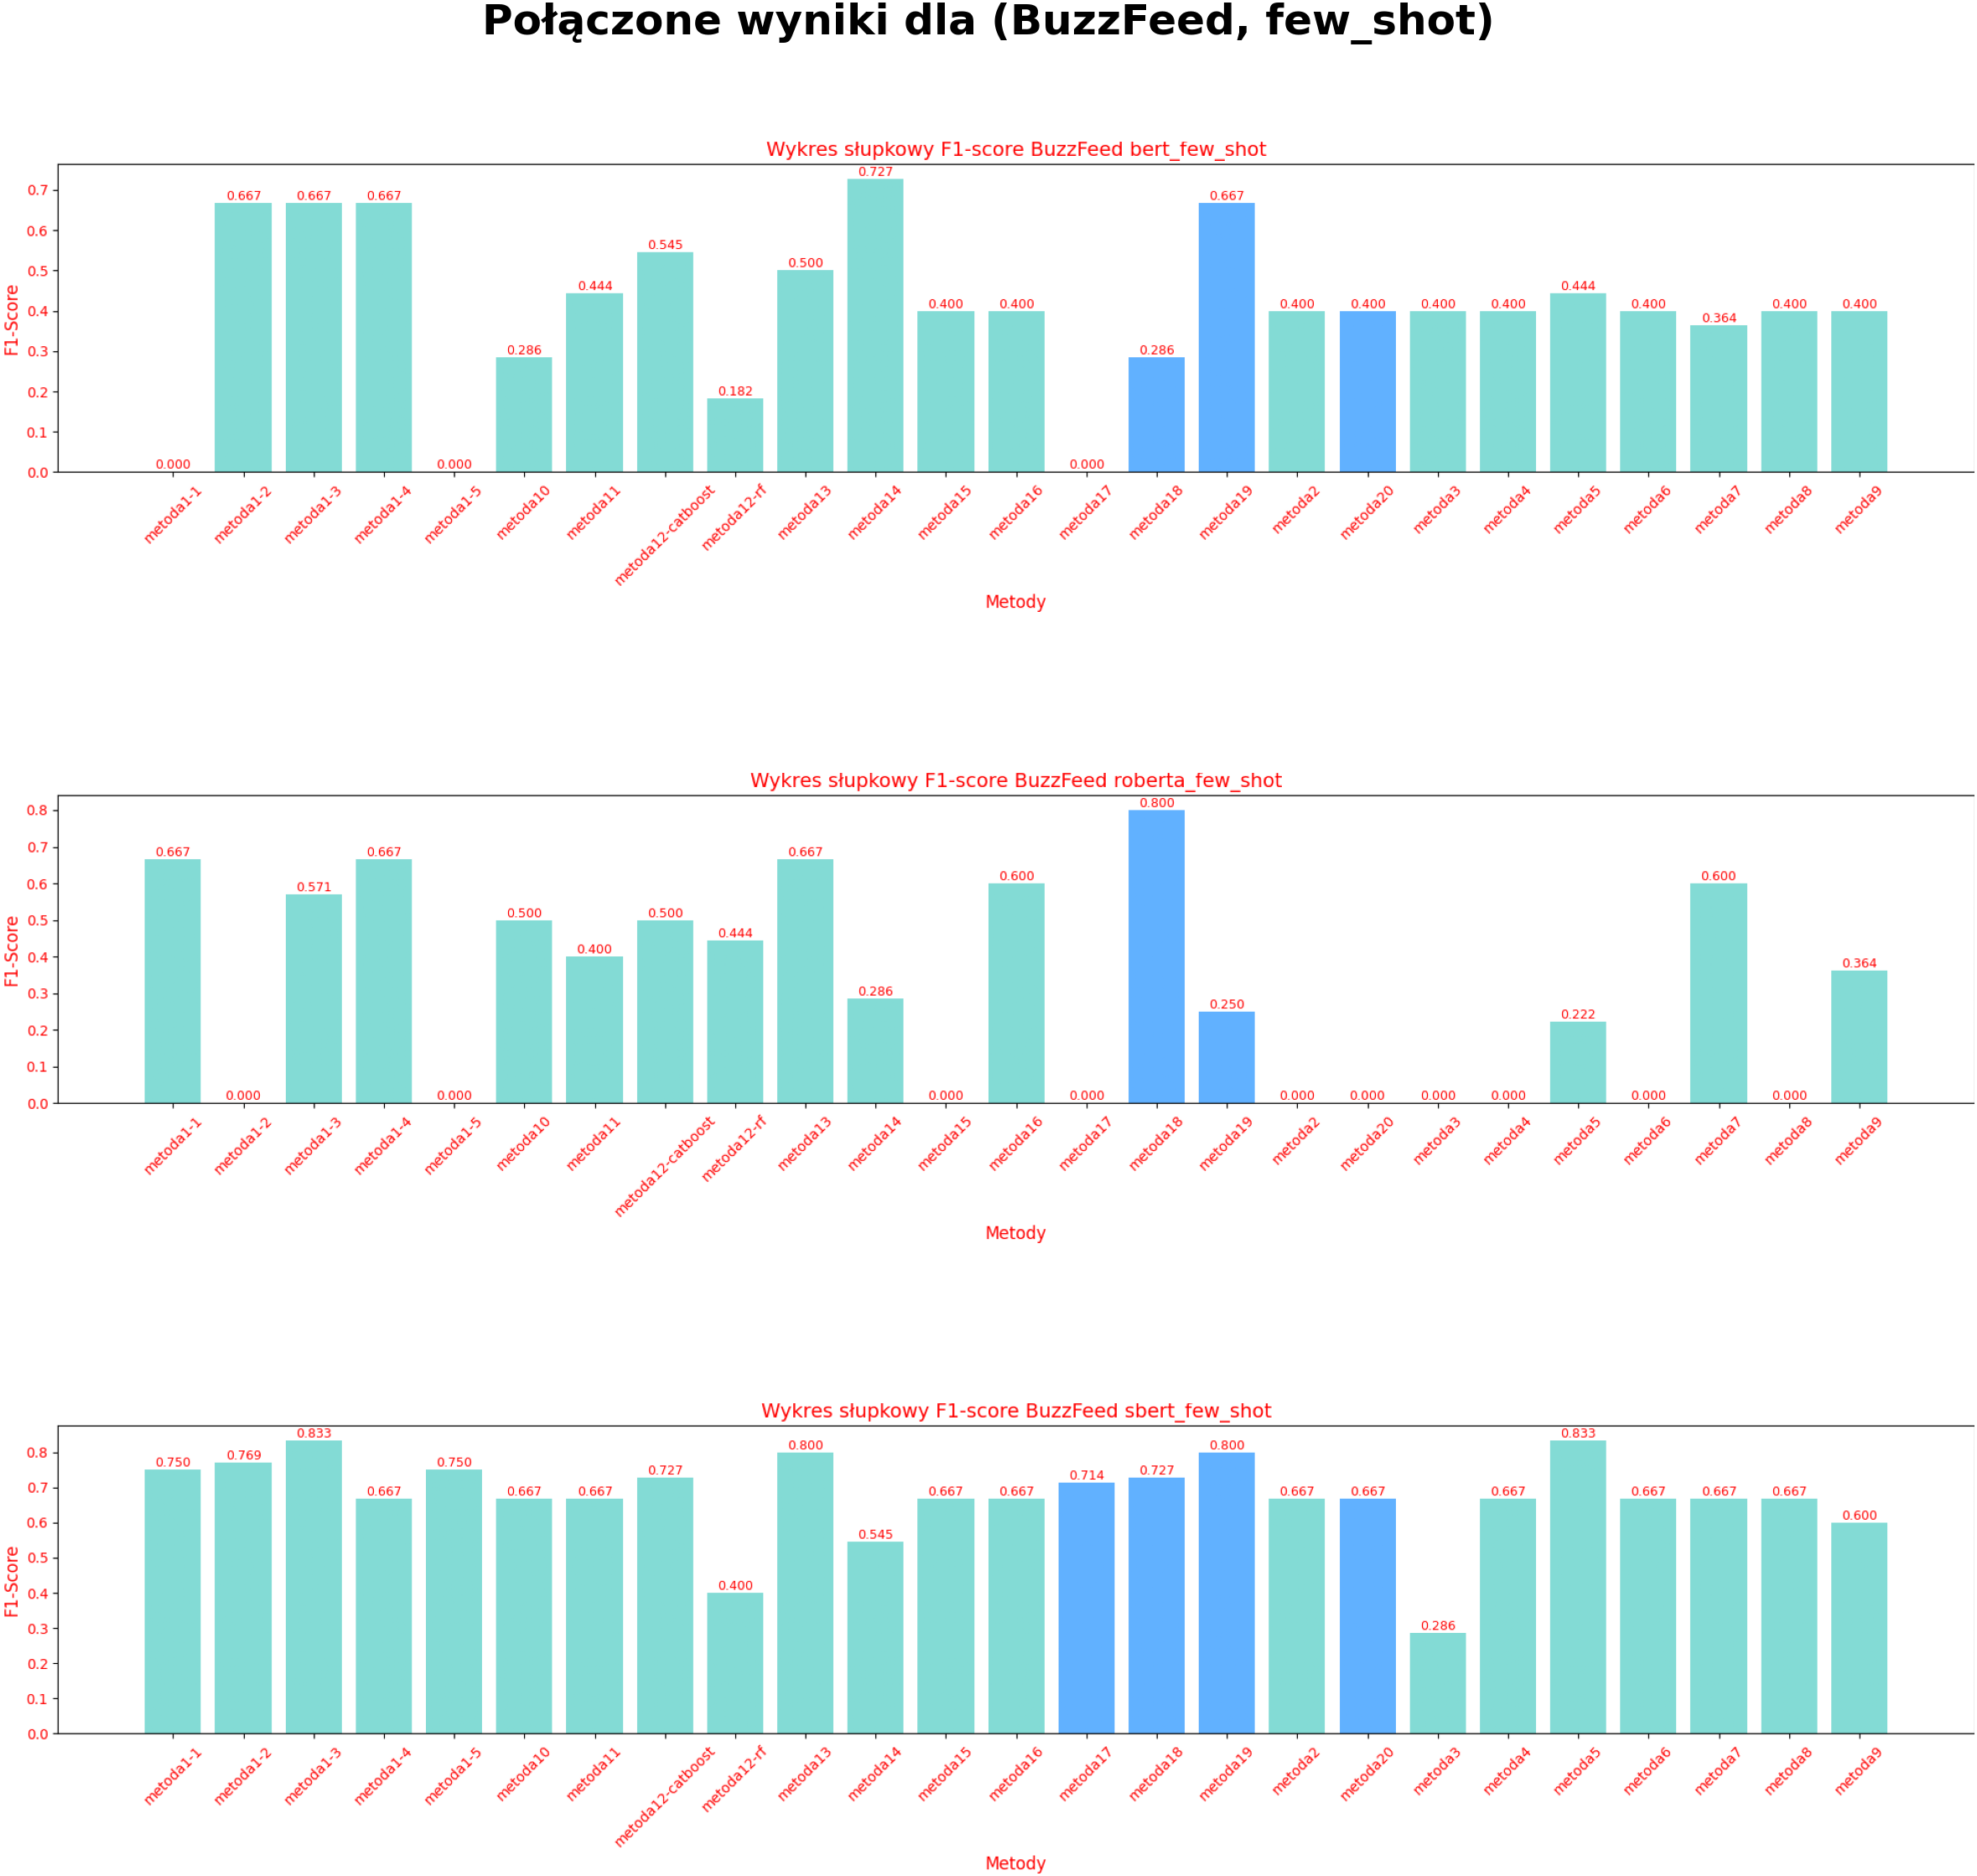
\includegraphics[width=0.99\textwidth]{img/stats/BuzzFeed_few_shot/BuzzFeed_few_shot_Combined_F1-Score_bar.png}
	\caption{Histogram rozkładu \textbf{Wyniku F1 (F1-Score)}.}
	\label{fig:buzzfeed_few_shot_f1}
\end{figure}

\subsubsection{ROC-AUC}
Wykresy ROC-AUC (\ref{fig:buzzfeed_few_shot_roc}) wskazują, że dla BERT \texttt{Metoda14} osiągnęła najwyższe wartości, a \texttt{Metoda16}, \texttt{Metoda20} najniższe. Dla RoBERTa \texttt{Metoda17}, \texttt{Metoda18} były najlepsze, a \texttt{Metoda19} najgorsza. Dla SBERT \texttt{Metoda19}, \texttt{Metoda5} osiągnęły wysokie wyniki, a \texttt{Metoda14} najniższe. \texttt{Metoda17} skuteczna dla RoBERTa dzięki VotingClassifier, \texttt{Metoda18} wysoka dla RoBERTa dzięki stacking, \texttt{Metoda19} słaba dla RoBERTa z braku optymalizacji, \texttt{Metoda20} słaba dla BERT z powodu prostej konfiguracji.

\begin{figure}[H]
	\centering
	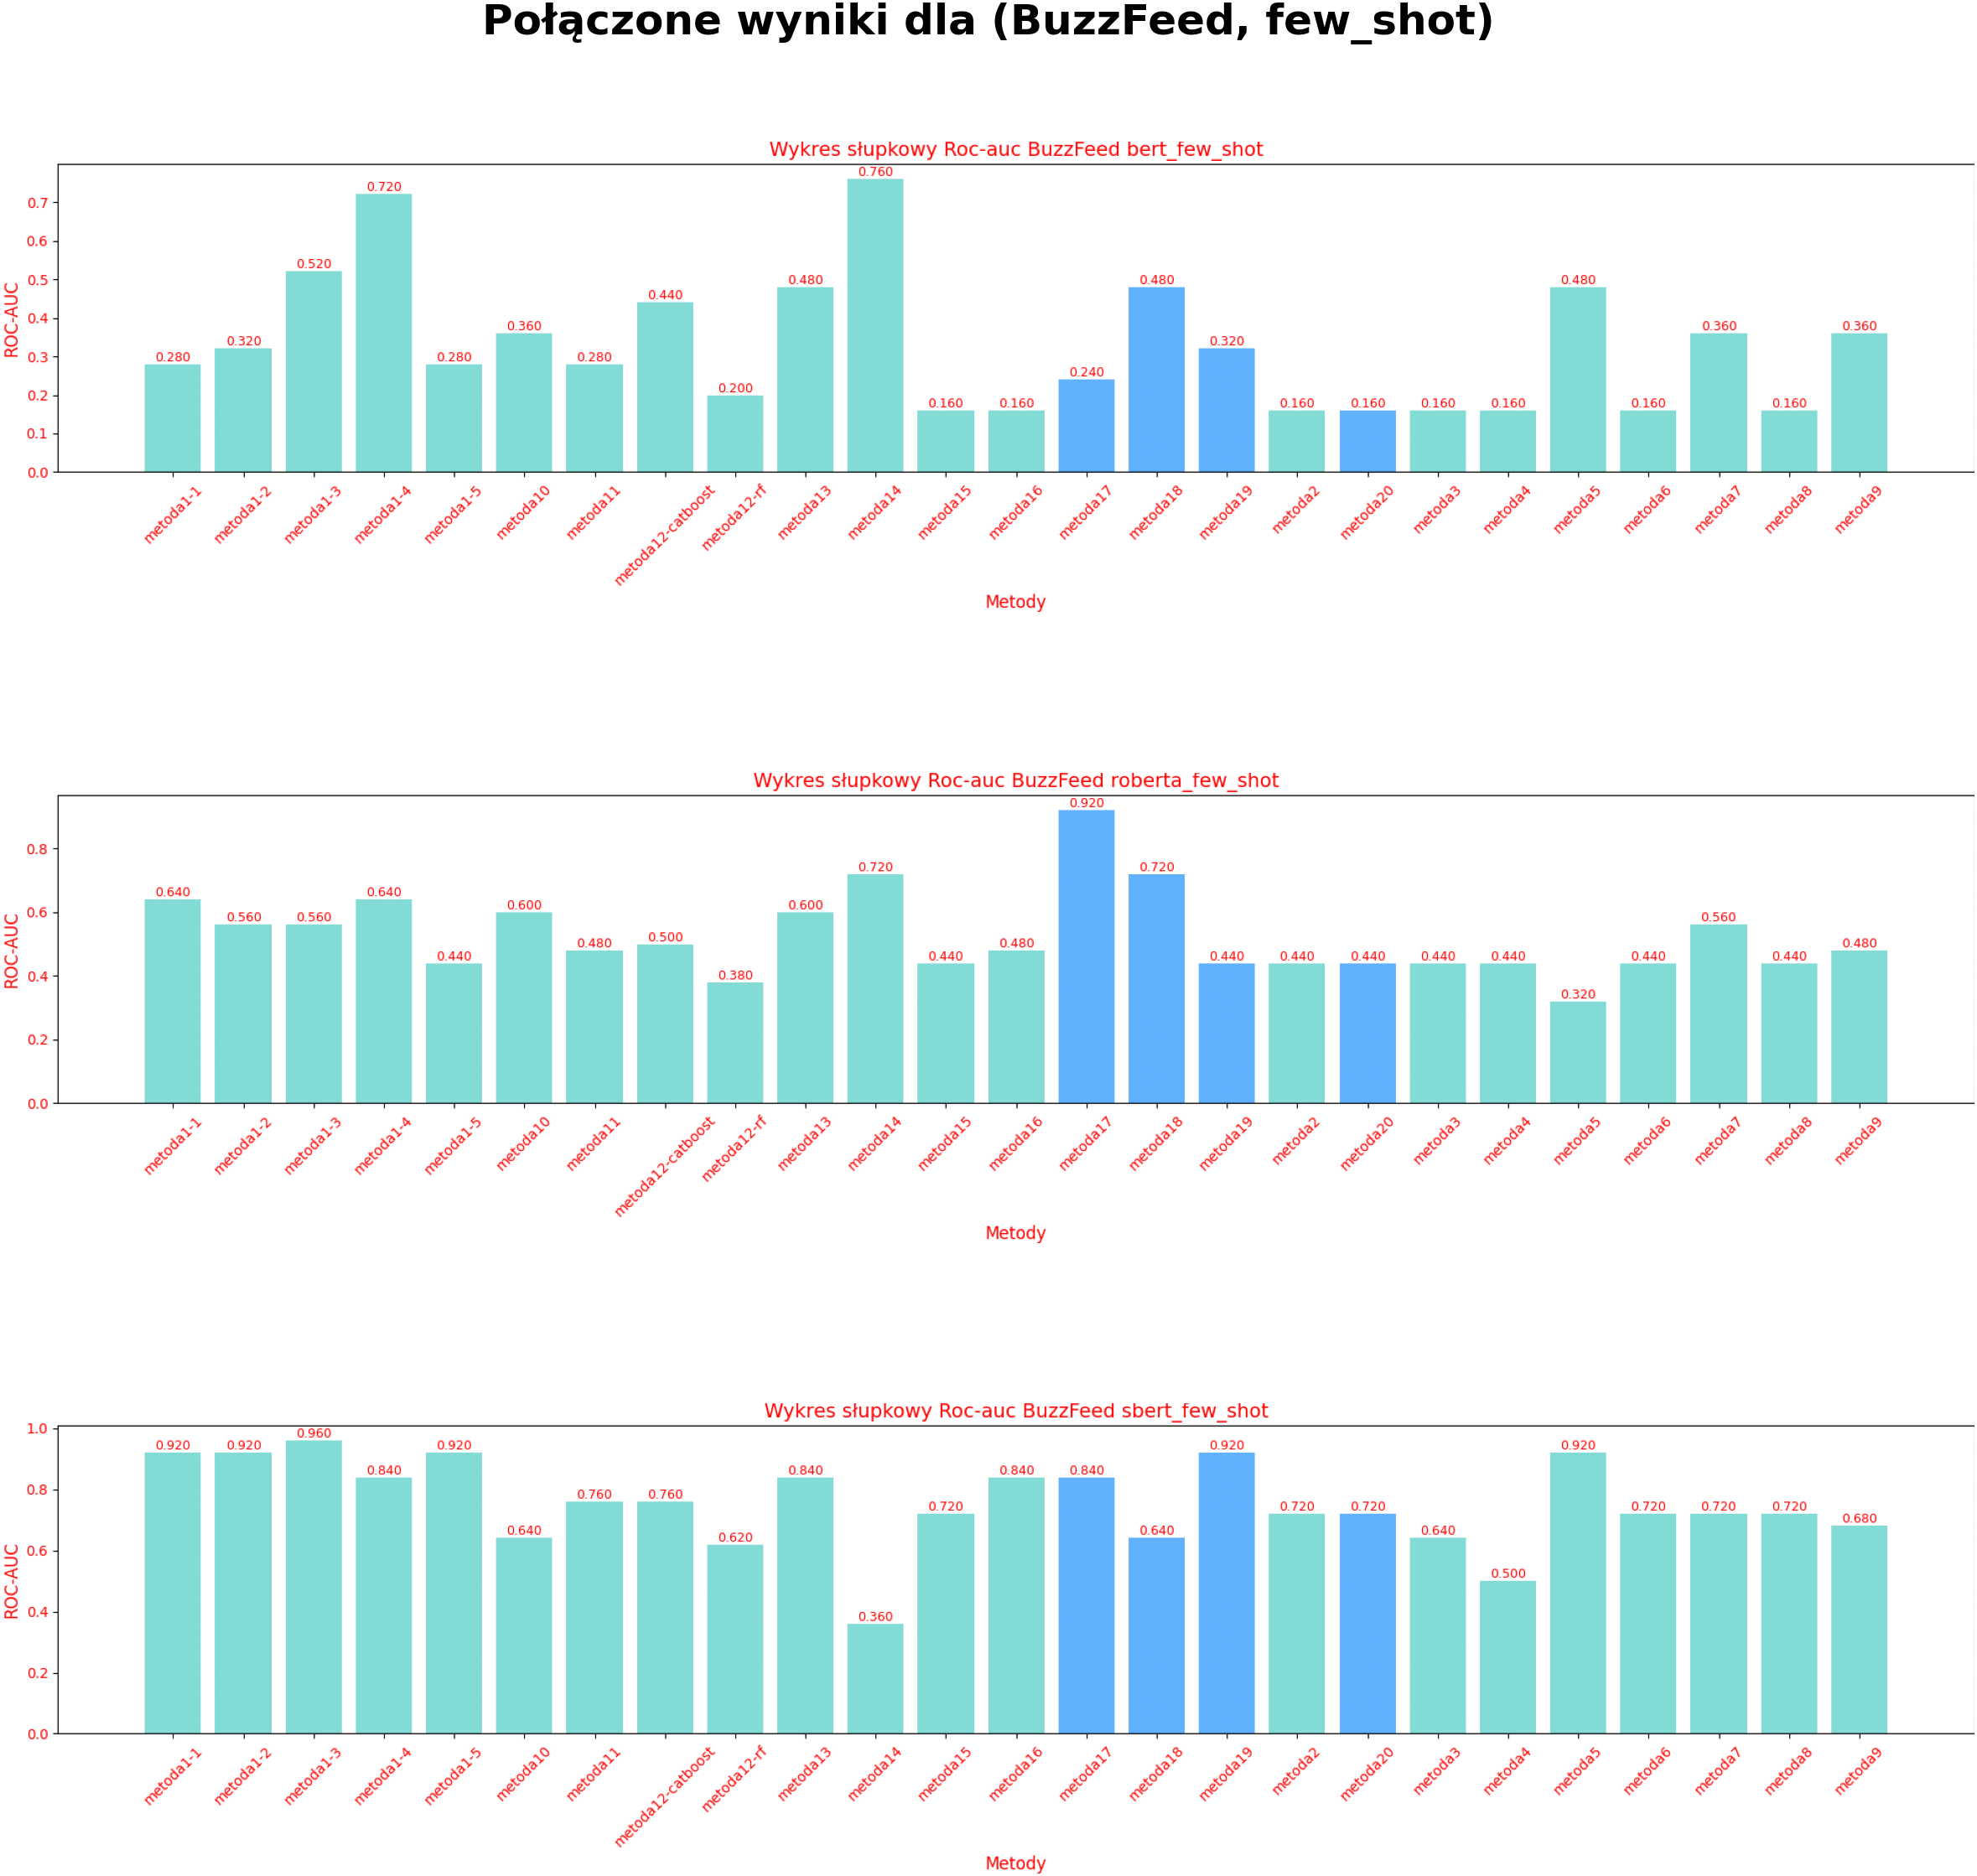
\includegraphics[width=0.99\textwidth]{img/stats/BuzzFeed_few_shot/BuzzFeed_few_shot_Combined_ROC-AUC_bar.png}
	\caption{Histogram rozkładu \textbf{Pola pod krzywą ROC-AUC (ROC-AUC)}.}
	\label{fig:buzzfeed_few_shot_roc}
\end{figure}

\subsection{Wyniki w trybie one-shot}

\subsubsection{Accuracy}
Wykresy Accuracy (\ref{fig:buzzfeed_one_shot_accuracy}) pokazują, że dla BERT \texttt{Metoda12-catboost}, \texttt{Metoda20} osiągnęły ~100\%, a pozostałe ~50\%. Dla RoBERTa \texttt{Metoda12-catboost}, \texttt{Metoda19} miały ~100\%, a reszta ~50\%. Dla SBERT \texttt{Metoda}1-1, \texttt{Metoda20} osiągnęły ~100\%, a inne ~50\%. \texttt{Metoda17}, \texttt{Metoda18}, \texttt{Metoda19} słabe dla BERT z powodu niedostatecznej adaptacji, \texttt{Metoda20} skuteczna dzięki zoptymalizowanemu LightGBM.

\begin{figure}[H]
	\centering
	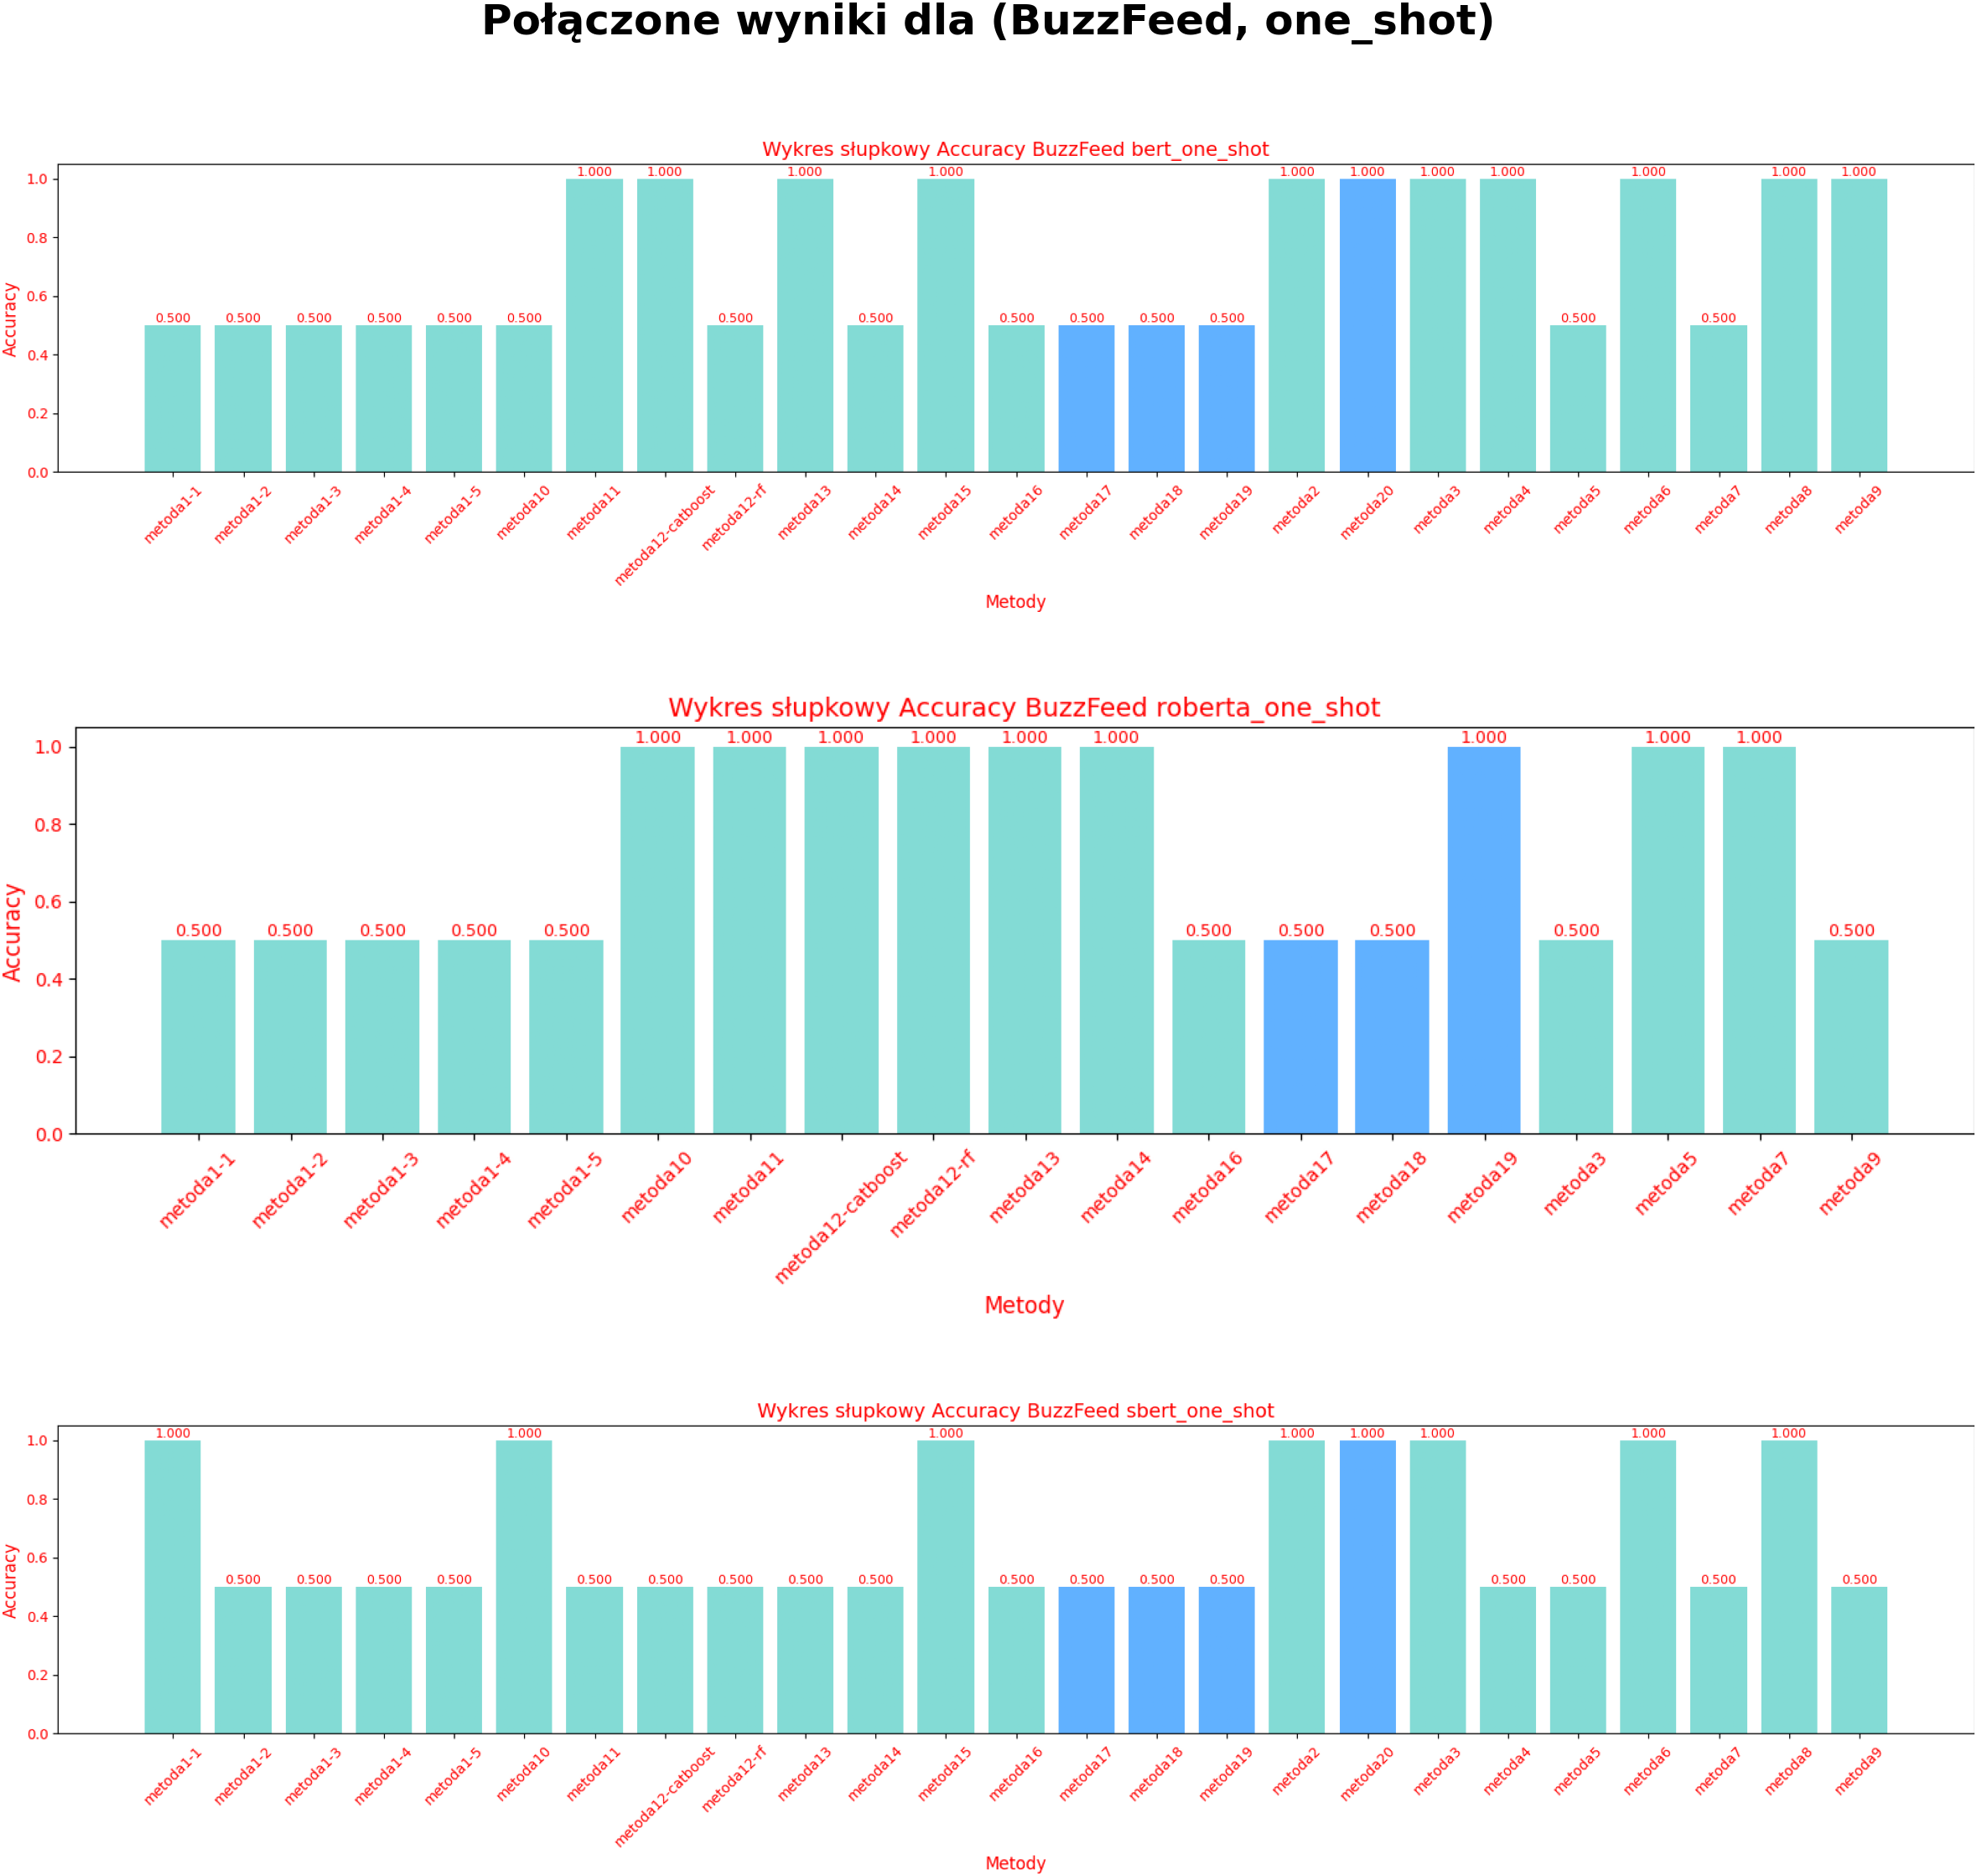
\includegraphics[width=0.99\textwidth]{img/stats/BuzzFeed_one_shot/BuzzFeed_one_shot_Combined_Accuracy_bar_chart.png}
	\caption{Histogram rozkładu \textbf{Dokładności (Accuracy)}.}
	\label{fig:buzzfeed_one_shot_accuracy}
\end{figure}

\subsubsection{F1-Score}
Wykresy F1-Score (\ref{fig:buzzfeed_one_shot_f1}) wskazują, że dla BERT \texttt{Metoda11}, \texttt{Metoda20} osiągnęły ~100\%, a \texttt{Metoda19}, \texttt{Metoda16} najniższe. Dla RoBERTa \texttt{Metoda12}, \texttt{Metoda19} miały ~100\%, a \texttt{Metoda1-4} najgorsza. Dla SBERT \texttt{Metoda1-1}, \texttt{Metoda20} osiągnęły ~100\%, a \texttt{Metoda18}, \texttt{Metoda19} najniższe. \texttt{Metoda17}, \texttt{Metoda18}, \texttt{Metoda19} słabe z powodu niedopasowania do one-shot, \texttt{Metoda20} skuteczna dzięki LightGBM.

\begin{figure}[H]
	\centering
	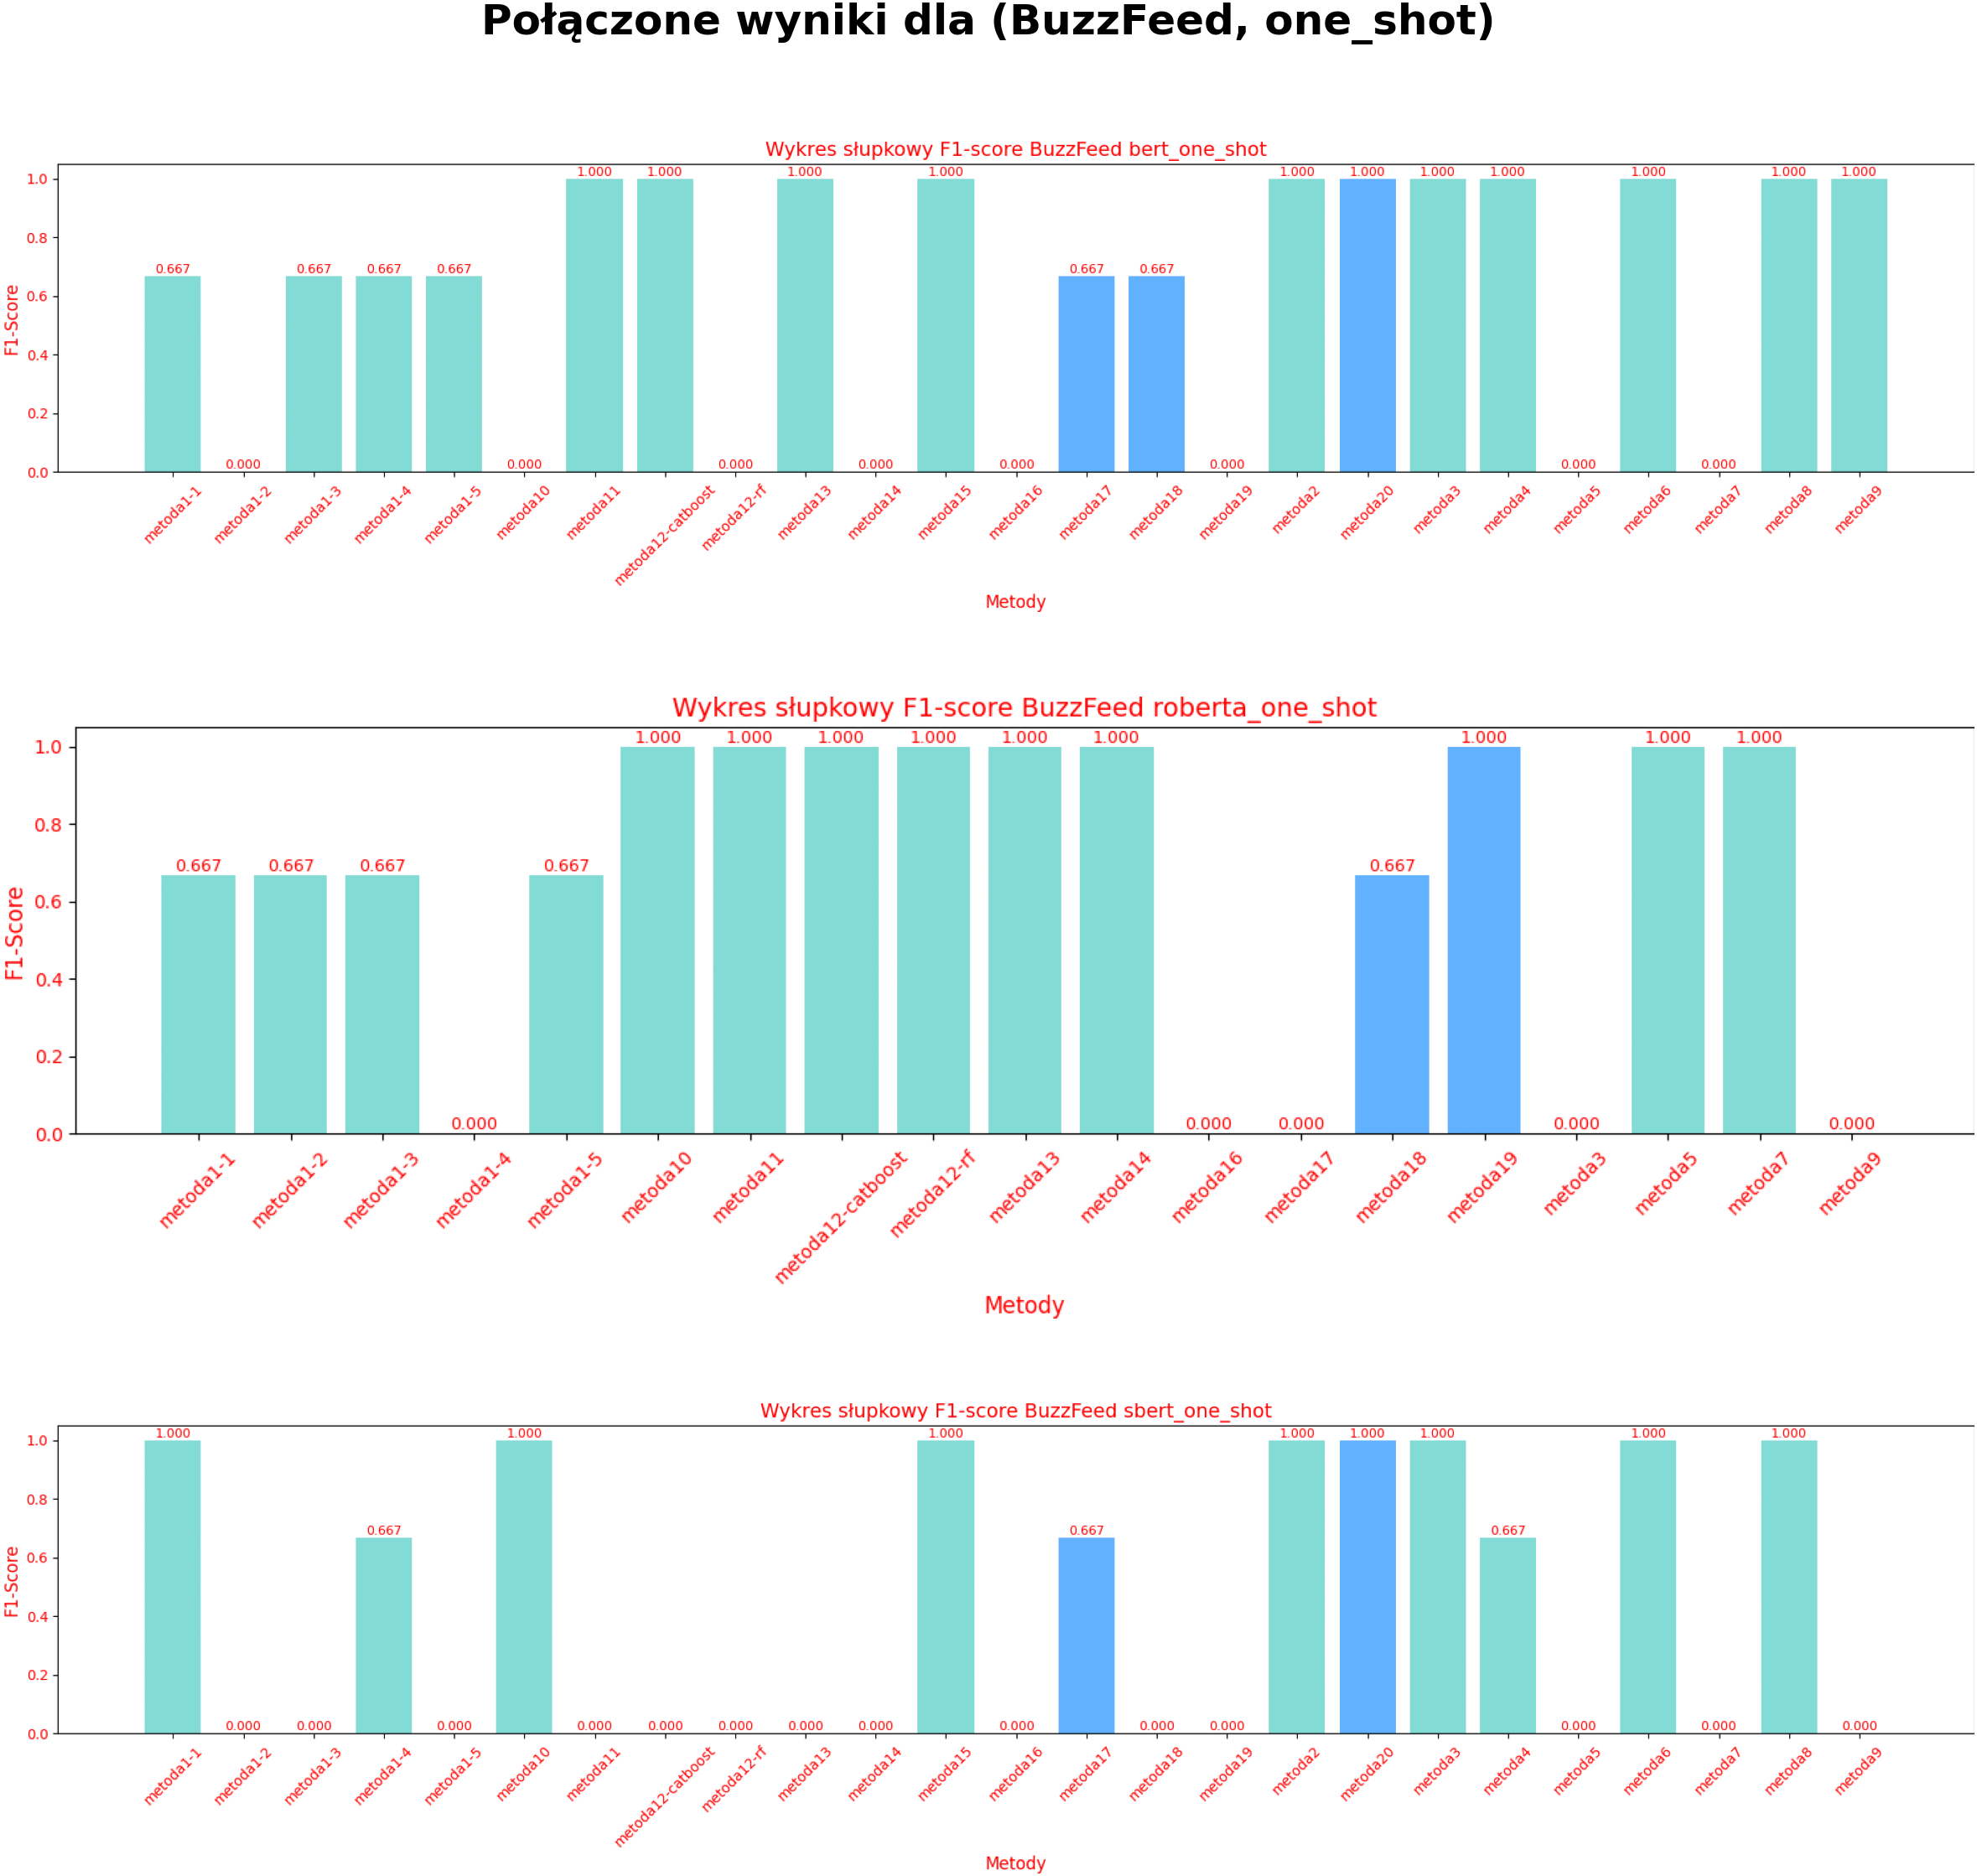
\includegraphics[width=0.99\textwidth]{img/stats/BuzzFeed_one_shot/BuzzFeed_one_shot_Combined_F1-Score_bar.png}
	\caption{Histogram rozkładu \textbf{Wyniku F1 (F1-Score)}.}
	\label{fig:buzzfeed_one_shot_f1}
\end{figure}

\subsubsection{ROC-AUC}
Wykresy ROC-AUC (\ref{fig:buzzfeed_one_shot_roc}) pokazują, że dla BERT \texttt{Metoda20}, \texttt{Metoda17} osiągnęły wysokie wyniki, a \texttt{Metoda18}, \texttt{Metoda19} najniższe. Dla RoBERTa \texttt{Metoda17}, \texttt{Metoda19} były najlepsze, a \texttt{Metoda1-x} najgorsze. Dla SBERT \texttt{Metoda20}, \texttt{Metoda11} osiągnęły wysokie wyniki, a \texttt{Metoda17}, \texttt{Metoda19} najniższe. \texttt{Metoda17} skuteczna dla RoBERTa dzięki VotingClassifier, \texttt{Metoda18} słaba dla BERT/SBERT z braku optymalizacji, \texttt{Metoda19} słaba dla SBERT z niedopasowania, \texttt{Metoda20} wysoka dzięki LightGBM.

\begin{figure}[H]
	\centering
	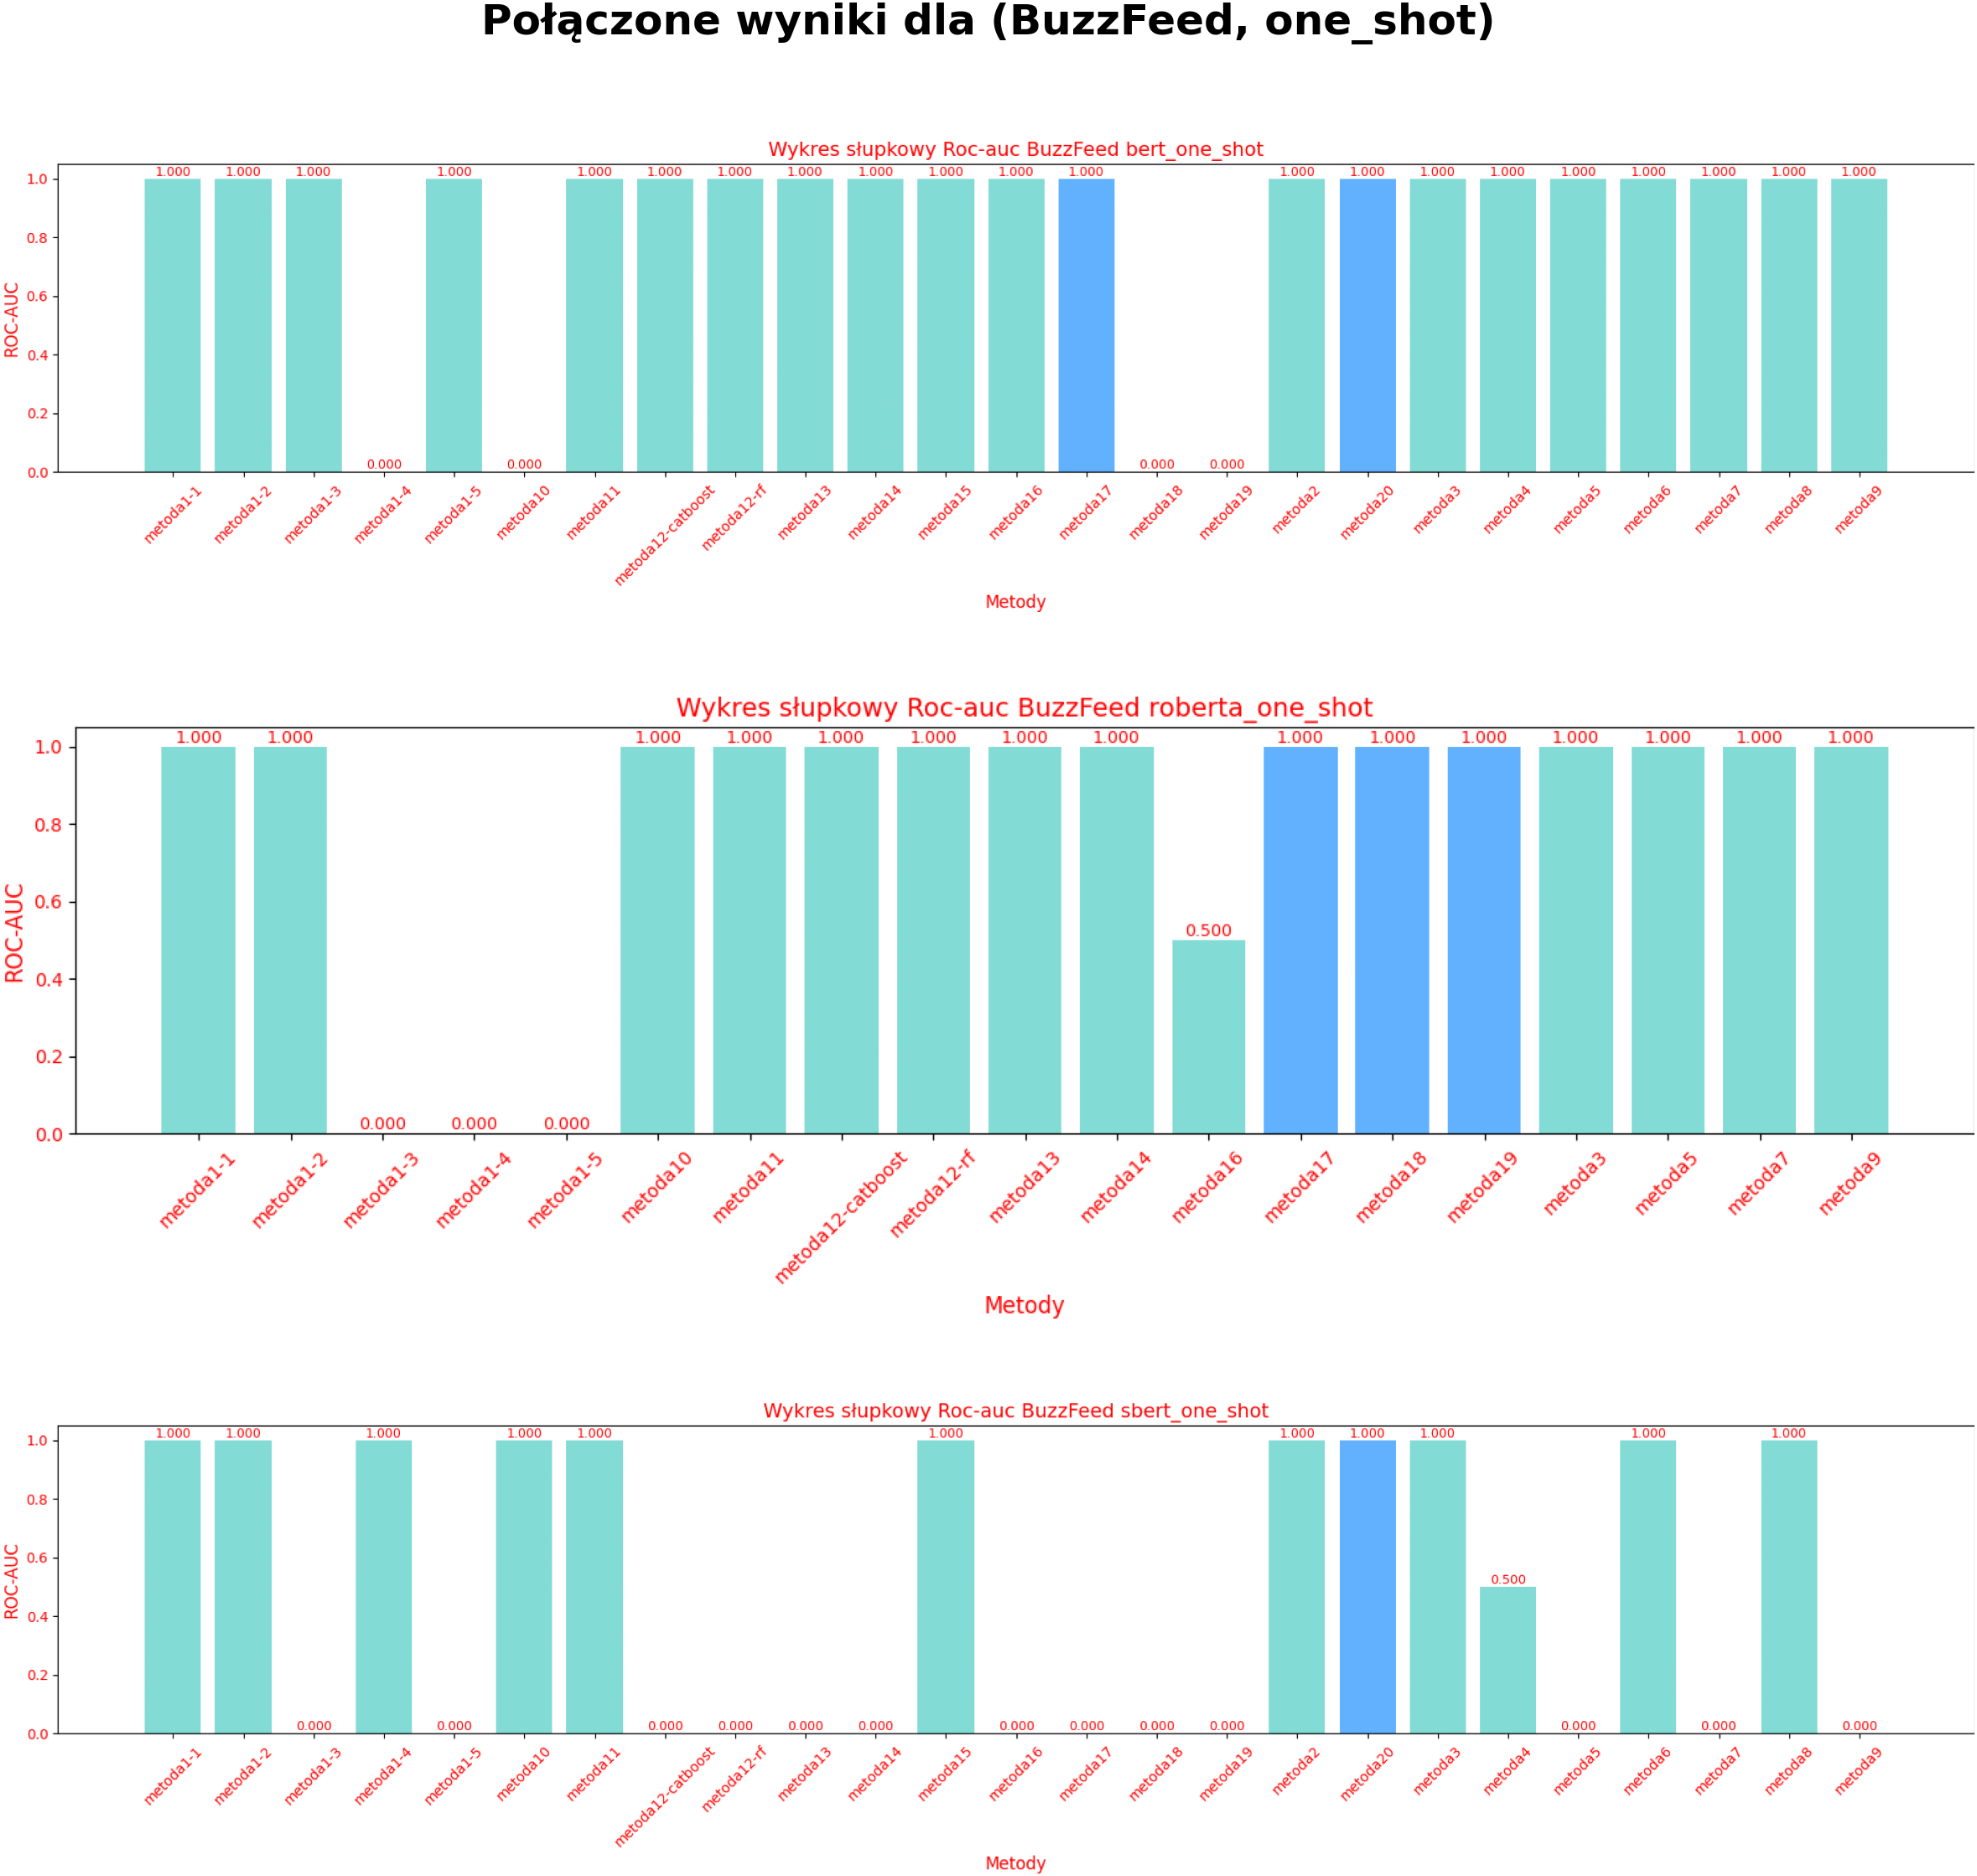
\includegraphics[width=0.99\textwidth]{img/stats/BuzzFeed_one_shot/BuzzFeed_one_shot_Combined_ROC-AUC_bar.png}
	\caption{Histogram rozkładu \textbf{Pola pod krzywą ROC-AUC (ROC-AUC)}.}
	\label{fig:buzzfeed_one_shot_roc}
\end{figure}

\subsection{Dodatkowa analiza wyników dla datasetu BuzzFeed}
\label{subsec:buzzfeed_additional_analysis}

\subsubsection{Wyniki AUC-PR}
Tabela \ref{tab:buzzfeed_auc_pr} przedstawia wyniki AUC-PR. Najwyższy wynik (0.7634) osiągnęła \texttt{metoda1-2}, a wśród metod autorskich \texttt{metoda17} (0.7041) była najlepsza. \texttt{Metoda17} skuteczna dzięki VotingClassifier, \texttt{Metoda18} (0.5893) słaba z powodu prostej konfiguracji, \texttt{Metoda19} (0.6182) średnia z braku balansowania, \texttt{Metoda20} (0.6671) dobra dzięki LightGBM.

\begin{table}[H]
	\centering
	\caption{Wyniki AUC-PR dla metod na datasecie BuzzFeed}
	\label{tab:buzzfeed_auc_pr}
	\begin{tabular}{l r}
		\toprule
		Metoda            & AUC-PR \\
		\midrule
		metoda1-1         & 0.7527 \\
		metoda1-2         & 0.7634 \\
		metoda1-3         & 0.6267 \\
		metoda1-4         & 0.6516 \\
		metoda1-5         & 0.5820 \\
		metoda2           & 0.6671 \\
		metoda3           & 0.6782 \\
		metoda4           & 0.6445 \\
		metoda5           & 0.6463 \\
		metoda6           & 0.6671 \\
		metoda7           & 0.6566 \\
		metoda8           & 0.6671 \\
		metoda9           & 0.6391 \\
		metoda10          & 0.6785 \\
		metoda11          & 0.7266 \\
		metoda12-catboost & 0.6762 \\
		metoda12-rf       & 0.6234 \\
		metoda13          & 0.6743 \\
		metoda14          & 0.6324 \\
		metoda15          & 0.6671 \\
		metoda16          & 0.6138 \\
		metoda17          & 0.7041 \\
		metoda18          & 0.5893 \\
		metoda19          & 0.6182 \\
		metoda20          & 0.6671 \\
		\bottomrule
	\end{tabular}
\end{table}

\subsubsection{Testy normalności i analizy statystyczne}
Testy Shapiro-Wilka wykazały, że większość metryk nie ma rozkładu normalnego (p-value < 0.05), z wyjątkiem ROC-AUC (p-value >= 0.05). Testy Kruskal-Wallisa nie wykazały istotnych różnic między metodami (p-value >= 0.05), co sugeruje porównywalną skuteczność.

\subsubsection{Analiza korelacji}
Macierze korelacji Pearsona i Spearmana ujawniły silne dodatnie zależności między Accuracy a Cohen's Kappa (0.9996 w Pearsonie, 0.9992 w Spearmanie), Accuracy a MCC (0.9974 w Pearsonie, 0.9907 w Spearmanie) oraz ROC-AUC a AUC-PR (0.9376 w Pearsonie, 0.9101 w Spearmanie). Brak ujemnych korelacji wskazuje na zgodność metryk.

\begin{table}[H]
	\centering
	\caption{Kluczowe współczynniki korelacji Pearsona}
	\label{tab:buzzfeed_pearson_correlations}
	\begin{tabular}{l r l}
		\toprule
		Para metryk               & Współczynnik Pearsona & Interpretacja         \\
		\midrule
		Accuracy -- Cohen's Kappa & 0.9996                & Bardzo silna dodatnia \\
		Accuracy -- MCC           & 0.9974                & Bardzo silna dodatnia \\
		MCC -- Cohen's Kappa      & 0.9977                & Bardzo silna dodatnia \\
		Precision -- F1-Score     & 0.8777                & Silna dodatnia        \\
		Recall -- F1-Score        & 0.7355                & Silna dodatnia        \\
		ROC-AUC -- AUC-PR         & 0.9376                & Bardzo silna dodatnia \\
		\bottomrule
	\end{tabular}
\end{table}

\begin{table}[H]
	\centering
	\caption{Kluczowe współczynniki korelacji Spearmana}
	\label{tab:buzzfeed_spearman_correlations}
	\begin{tabular}{l r l}
		\toprule
		Para metryk               & Współczynnik Spearmana & Interpretacja         \\
		\midrule
		Accuracy -- Cohen's Kappa & 0.9992                 & Bardzo silna dodatnia \\
		Accuracy -- MCC           & 0.9907                 & Bardzo silna dodatnia \\
		MCC -- Cohen's Kappa      & 0.9868                 & Bardzo silna dodatnia \\
		Precision -- F1-Score     & 0.8147                 & Silna dodatnia        \\
		Recall -- F1-Score        & 0.7760                 & Silna dodatnia        \\
		ROC-AUC -- AUC-PR         & 0.9101                 & Bardzo silna dodatnia \\
		\bottomrule
	\end{tabular}
\end{table}

\subsection{Podsumowanie wniosków}
Analiza wyników dla datasetu BuzzFeed pokazuje, że zaawansowane modele ensemble, takie jak \texttt{Metoda12-catboost}, \texttt{Metoda13}, \texttt{Metoda19}, \texttt{Metoda20}, osiągają wysoką skuteczność w trybach klasycznym, few-shot i one-shot, szczególnie dla embeddingów RoBERTa i SBERT. W trybie one-shot RoBERTa i SBERT umożliwiają perfekcyjne wyniki (~100\% Accuracy i F1-Score), podczas gdy BERT jest mniej skuteczny (~50\% dla wielu metod). \texttt{Metoda17} (VotingClassifier) jest skuteczna dla RoBERTa, ale słaba dla BERT z powodu niedopasowania hiperparametrów. \texttt{Metoda18} (stacking z CatBoost) dominuje dla RoBERTa w trybie few-shot, ale zawodzi dla BERT z powodu prostej konfiguracji. \texttt{Metoda19} (stacking) osiąga wysokie wyniki dla BERT/SBERT dzięki zoptymalizowanemu łączeniu modeli, ale jest słaba dla RoBERTa z braku optymalizacji. \texttt{Metoda20} (LightGBM) jest skuteczna w trybie one-shot dzięki zoptymalizowanym modelom, ale średnia w innych trybach z powodu braku balansowania klas. Prostsze modele (\texttt{Metoda1-x}) są zróżnicowane, osiągając dobre wyniki dla SBERT, ale słabsze dla BERT. Wysoka kontrastowość klas w BuzzFeed \cite{Frost2016photon} ułatwia klasyfikację dla zoptymalizowanych metod, ale wymaga precyzyjnej konfiguracji w trudniejszych scenariuszach.
\section{Analiza wyników dla datasetu \textbf{ISOT}}
\label{subsec:isot_analysis}

W tej sekcji przedstawiono analizę wyników uzyskanych dla datasetu \textbf{ISOT} po przetestowaniu w trzech trybach podziału danych: \textbf{klasycznym}, \textbf{few\-shot} oraz \textbf{one\-shot}. Wyniki podzielono na podrozdziały według trybów uczenia, co ułatwia ich analizę i porównanie.

\subsection{Wyniki w trybie klasycznym}
W trybie \textbf{klasycznym} dla datasetu \textbf{ISOT}. Poniżej przedstawiono szczegółowy opis wyników w formie histogramów, które ilustrują rozkłady kluczowych metryk, oraz wykresu liniowego czasu wykonania eksperymentów.

\subsubsection{Accuracy}
Wykresy słupkowe \textbf{Dokładności (Accuracy)} \ref{fig:isot_classic_accuracy} pokazują rozkład wartości dokładności dla wszystkich metod. Analizując podany wykres słupkowy można zauważyć następujące rozkłady wyników:

\begin{itemize}
	\item \textbf{Wykres górny (BERT):}
	      \begin{itemize}
		      \item Najlepsze wyniki osiągnęły metody takie jak \texttt{Metoda14}, \texttt{Metoda16} oraz autorska \texttt{Metoda19}. Ich wysoka skuteczność wskazuje, że zaawansowane techniki ensemble learning są w stanie efektywnie wykorzystać bogate i złożone cechy generowane przez model BERT, osiągając wysoką dokładność w klasyfikacji.
		      \item Najgorsze wyniki odnotowano dla autorskiej \texttt{Metoda20}, zaawansowany model ensemble, co jest zaskakujące w porównaniu do jej wydajności w innych scenariuszach. \texttt{Metoda15} oraz \texttt{Metoda2}, trenująca model wykorzystując GradientBoosting oraz MLP na oddzielnych podzbiorach cech i łączy je za pomocą Regresji Logistycznej, \texttt{Metoda3}, \texttt{Metoda6}. Niska dokładność tych metod może świadczyć o niedostatecznej optymalizacji hiperparametrów dla embeddingów BERT, oraz o tym, że ich architektura nie jest w stanie odpowiednio przetworzyć złożoności danych z BERT w kontekście klasycznej walidacji.
	      \end{itemize}

	\item \textbf{Wykres środkowy (RoBERTa):}
	      \begin{itemize}
		      \item Najlepsze wyniki uzyskały metody \texttt{Metoda12-rf}, \texttt{Metoda13}, \texttt{Metoda14} oraz autorska \texttt{Metoda19} (model stackingowy). Wysoka skuteczność tych metod sugeruje, że embeddingi RoBERTa są dobrze dopasowane do zaawansowanych technik ensemble, a nawet do Random Forest w \texttt{Metoda12-rf}, pozwalając tym metodom na efektywne wykorzystanie złożonych wzorców w danych i osiągnięcie wysokiej dokładności.
		      \item Najgorsze wyniki wystąpiły dla autorskiej \texttt{Metoda17}. Niska dokładność tej metody, która jest złożonym modelem ensemble, może wskazywać na jej specyficzne trudności w generalizacji dla embeddingów RoBERTa.
	      \end{itemize}

	\item \textbf{Wykres dolny (SBERT):}
	      \begin{itemize}
		      \item Najlepsze wyniki to między innymi dla metod z grupy \texttt{Metoda1}, większości innych metod i autorskich \texttt{Metoda17} oraz \texttt{Metoda18}. Ta szeroka gama metod osiągających wysokie wyniki pokazuje, że embeddingi SBERT dostarczają wysoce informatywnych cech, które mogą być efektywnie przetwarzane zarówno przez zaawansowane ensemble, jak i dobrze zoptymalizowane, prostsze architektury.
		      \item Najgorsze wyniki odnotowano dla \texttt{Metoda4}. Niska dokładność tej metody może sugerować, że mimo jej złożonej struktury, konfiguracja lub proces optymalizacji dla embeddingów SBERT nie były wystarczająco efektywne, co skutkuje słabą zdolnością klasyfikacji.
	      \end{itemize}
\end{itemize}

Analiza wykresów słupkowych dokładności dla klasycznego uczenia ujawnia, że modele oparte na ensemble learning, takie jak stacking (\texttt{Metoda14}, \texttt{Metoda16}, \texttt{Metoda19}, \texttt{Metoda13}, \texttt{Metoda18}) oraz VotingClassifier (\texttt{Metoda17}), mają duży potencjał do osiągania wysokiej dokładności. Ich wydajność jest jednak silnie uzależniona od właściwego doboru modeli bazowych i starannej optymalizacji hiperparametrów, co jest widoczne w zróżnicowanych wynikach dla różnych typów embeddingów (przykładowo \texttt{Metoda14} i \texttt{Metoda16} radzą sobie świetnie z BERT, ale \texttt{Metoda16} odnotowuje niskie wyniki dla SBERT). Prostsze modele, a nawet indywidualne instancje sieci neuronowych (\texttt{Metoda1-x}), czasami wykazują obiecujące wyniki (szczególnie dla SBERT). Kluczowe jest również uwzględnienie specyfiki każdego typu embeddingu językowego, gdyż optymalna metoda dla jednego embeddingu niekoniecznie sprawdzi się dla innego.

Wśród autorskich metod, \texttt{Metoda19} osiąga bardzo dobre wyniki dla osadzeń BERT i RoBERTa. \texttt{Metoda17} i \texttt{Metoda18} wyróżniają się dla SBERT. Z kolei \texttt{Metoda20} posiada słabe wyniki dla BERT, a \texttt{Metoda17} dla RoBERTa, co podkreśla konieczność precyzyjnej optymalizacji metod autorskich pod kątem specyfiki każdego typu embeddingu. Dalsze badania i optymalizacja są niezbędne, aby mogły w pełni wykorzystać swój potencjał.
\begin{figure}[H]
	\centering
	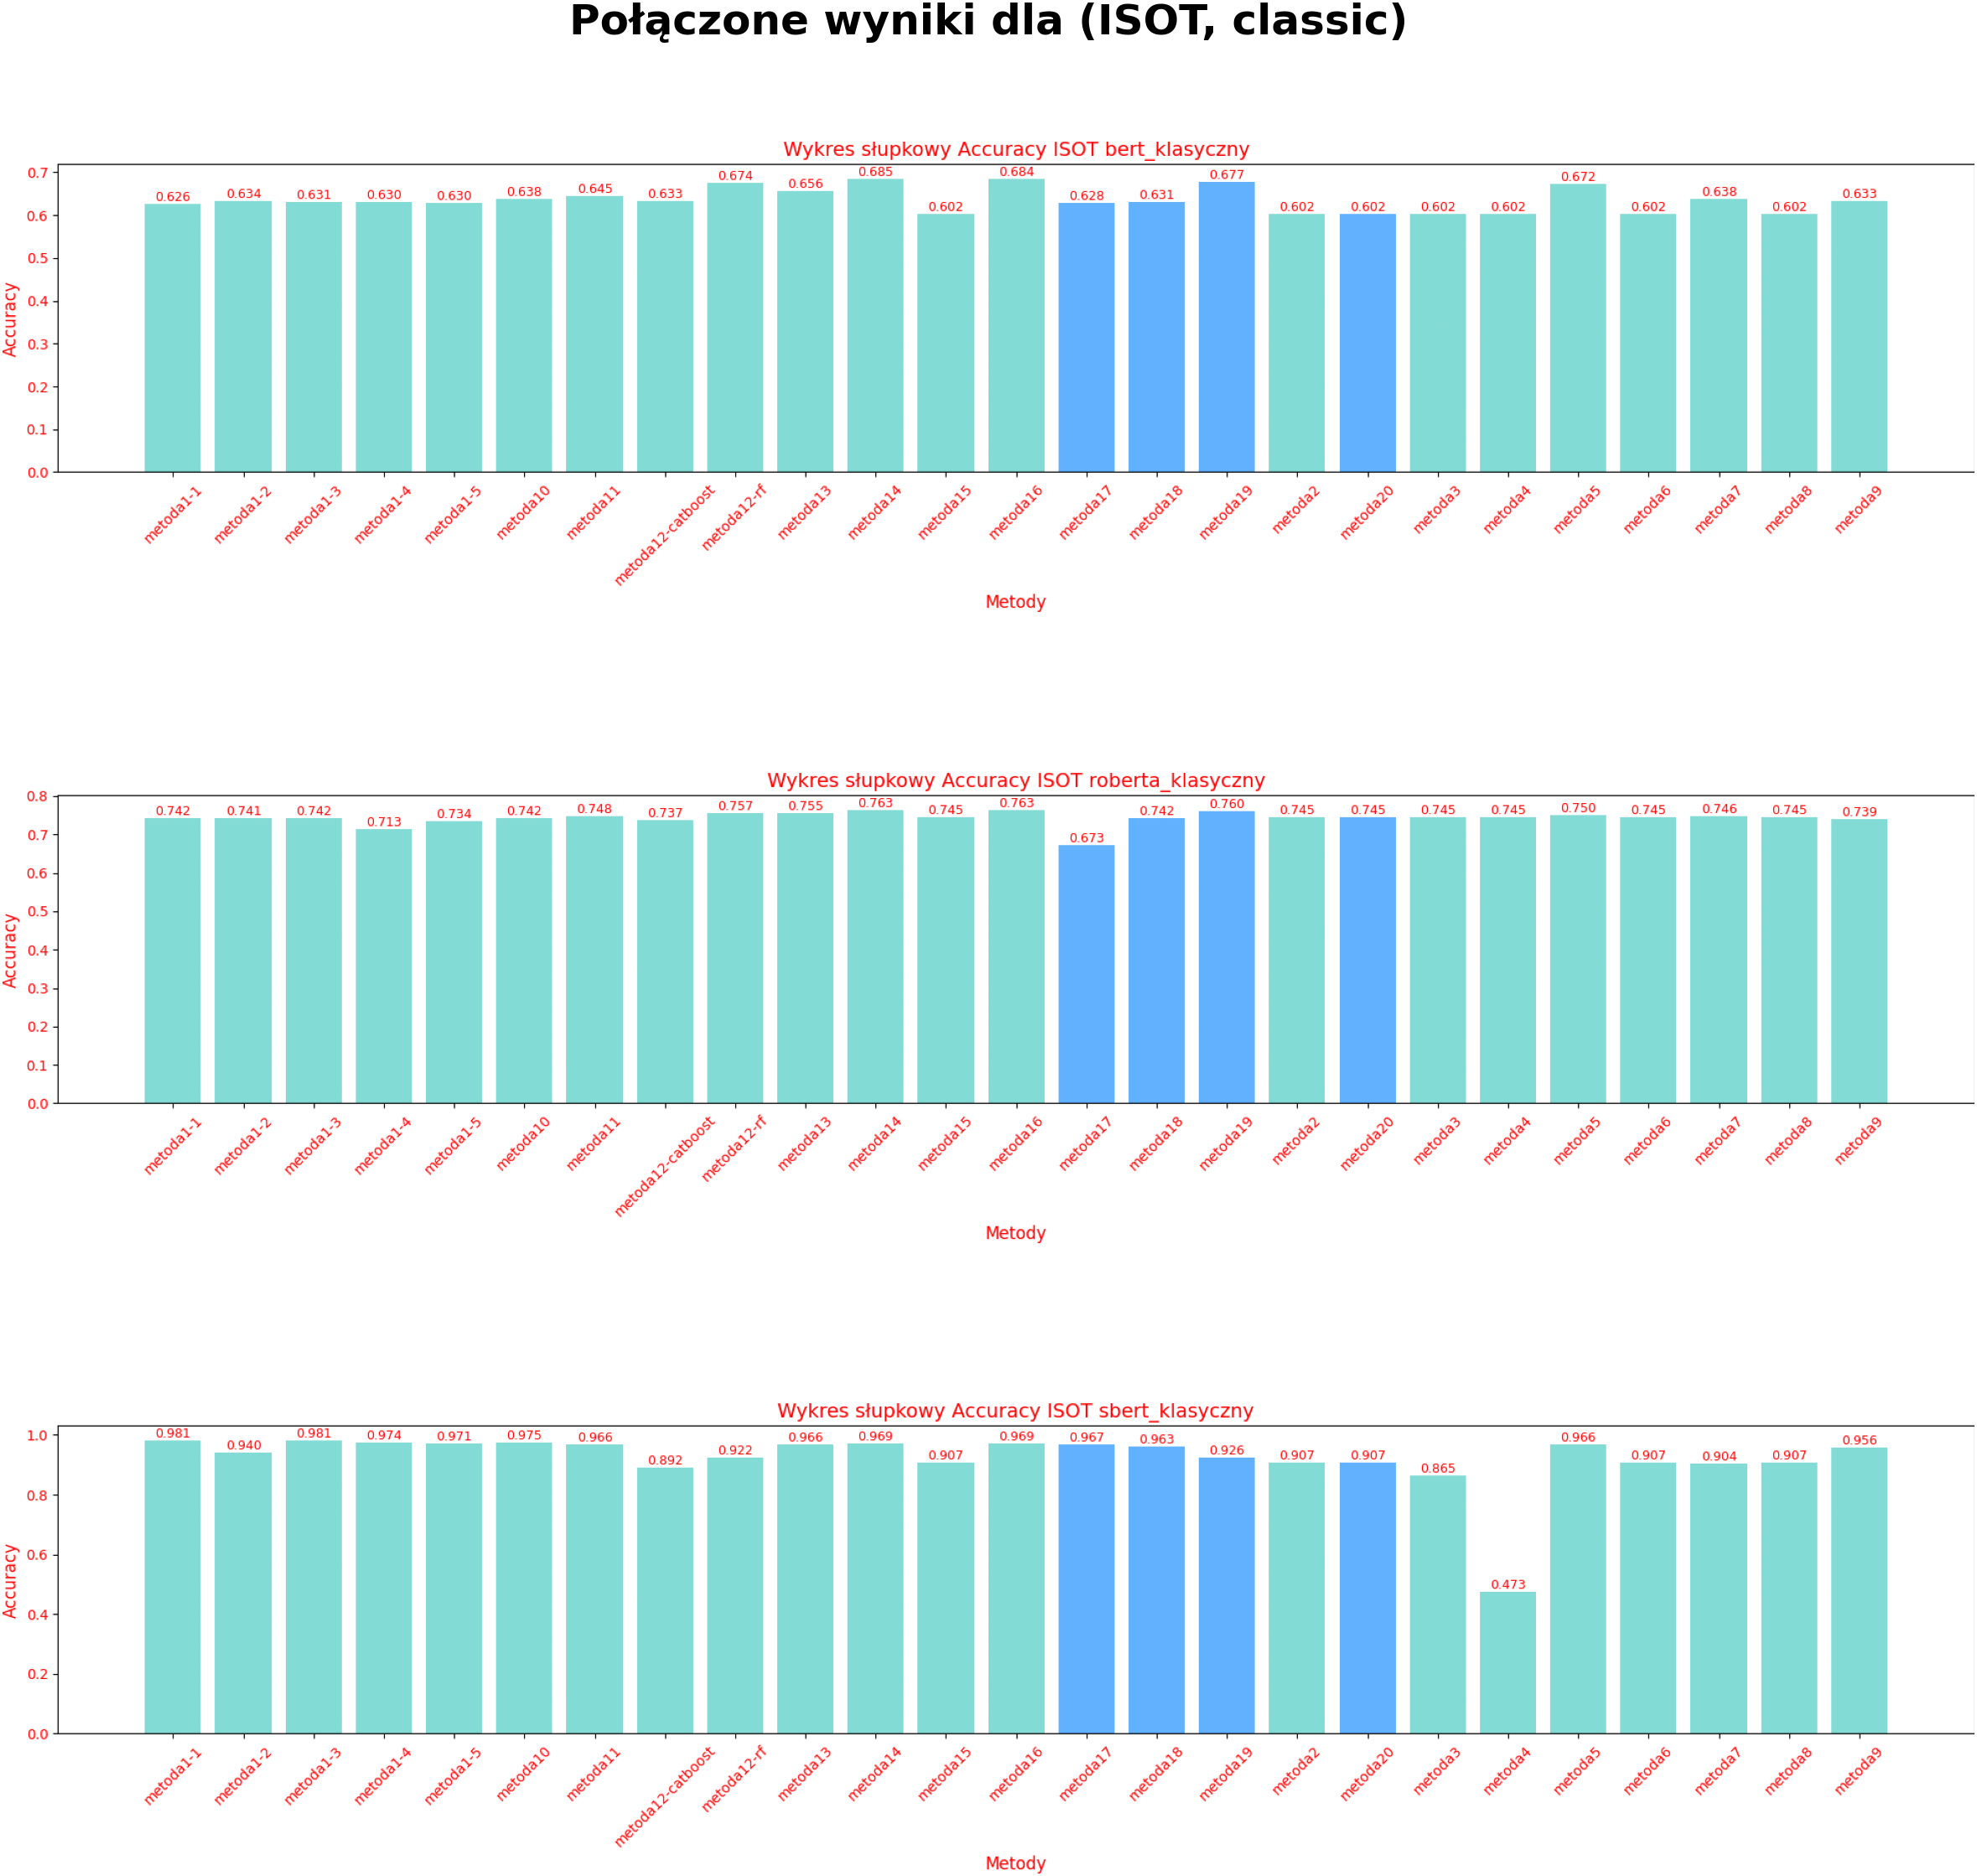
\includegraphics[width=0.99\textwidth]{img/stats/ISOT_classic/ISOT_classic_Combined_Accuracy_bar_chart.png}
	\caption{Histogram rozkładu \textbf{Dokładności (Accuracy)}.}
	\label{fig:isot_classic_accuracy}
\end{figure}

\subsubsection{F1-Score}
Wykresy słupkowe \textbf{Wyniku F1 (F1-Score)} \ref{fig:isot_classic_f1} przedstawiają rozkład wartości F1-Score dla wszystkich analizowanych metod. Na podstawie wykresu można sformułować następujące obserwacje:

\begin{itemize}
	\item \textbf{Wykres górny (BERT):}
	      \begin{itemize}
		      \item Najwyższe wartości F1-Score osiągnęły metody takie jak \texttt{Metoda14} (model zespołowy stacking z użyciem Random Forest, AdaBoost i SVC jako bazowych oraz Logistic Regression jako finalnego estymatora), \texttt{Metoda16} (model zespołowy stacking z meta-klasyfikatorem używającym regresji logistycznej, bazujące na Random Forest i SVC) oraz moja implementacja \texttt{Metoda19} (model stackingowy). Ich wysoka skuteczność wskazuje na to, że zaawansowana technika stacking jest w stanie efektywnie wykorzystać bogate i złożone cechy generowane przez model BERT, osiągając zbalansowane wyniki między precyzją a recall.
		      \item Najniższe wyniki odnotowano dla \texttt{Metoda1-4}, \texttt{Metoda15}, \texttt{Metoda2} ponieważ trenuje model wykorzystując GradientBoosting oraz MLP na oddzielnych podzbiorach cech i łączy je za pomocą Regresji Logistycznej. Dodatkowo \texttt{Metoda3} jako dwupoziomowy model zespołowy z VotingClassifier i Bagging/AdaBoost, \texttt{Metoda4} z architekturą opartą na zespole sieci Bi-LSTM, CNN i MLP oraz autorska \texttt{Metoda20} posiadają słabe wyniki. Niska wartość F1-Score dla tych metod, w tym dla niektórych złożonych modeli ensemble, może świadczyć o tym, że ich architektura prowadzi do niezbalansowanej wydajności precyzji i recall w kontekście klasycznej walidacji.
	      \end{itemize}
	\item \textbf{Wykres środkowy (RoBERTa):}
	      \begin{itemize}
		      \item Najlepsze rezultaty uzyskały metody z grupy \texttt{Metoda1} , \texttt{Metoda13} (wykorzystująca technikę SMOTETomek oraz zaawansowany stacking z Random Forest, Gradient Boosting i XGBoost), \texttt{Metoda14} (model zespołowy stacking z Random Forest, AdaBoost i SVC), \texttt{Metoda16} (model zespołowy stacking z meta-klasyfikatorem) oraz autorska \texttt{Metoda19}. Wysoka skuteczność tych metod sugeruje, że embeddingi RoBERTa są dobrze dopasowane do zaawansowanych technik ensemble, a także do prostszych sieci neuronowych, pozwalając tym metodom na efektywne wykorzystanie złożonych wzorców w danych i osiągnięcie zbalansowanych wyników klasyfikacji.
		      \item Najsłabsze wyniki wykazała \texttt{Metoda1-4}. Niska wartość F1-Score dla tej metody może wskazywać na to, że jej konfiguracja jest nie optymalna dla tego typu danych.
	      \end{itemize}
	\item \textbf{Wykres dolny (SBERT):}
	      \begin{itemize}
		      \item Najlepsze wartości F1-Score osiągnęły \texttt{Metoda13} (stacking z SMOTETomek), \texttt{Metoda14} (stacking z Random Forest, AdaBoost i SVC), \texttt{Metoda9}, \texttt{Metoda5} (model stackingowy z Random Forest i XGBoost jako bazowymi oraz Logistic Regression jako meta-modelem) oraz również autorskie \texttt{Metoda17} (zaawansowany VotingClassifier) i \texttt{Metoda18} (stacking z GradientBoosting i CatBoost). Embeddingi SBERT dostarczają wiele informatywnych cech, które mogą być efektywnie przetwarzane zarówno przez zaawansowane ensemble, jak i dobrze zoptymalizowane, prostsze architektury, osiągając zbalansowaną wydajność.
		      \item Najgorsze rezultaty zaobserwowano dla \texttt{Metoda4}. Niska wartość F1-Score dla tej metody może sugerować, że mimo jej złożonej struktury, konfiguracja lub proces optymalizacji dla embeddingów SBERT nie były wystarczająco efektywne, co skutkuje niezbalansowaną wydajnością precyzji i recall.
	      \end{itemize}
\end{itemize}

Analiza wykresów słupkowych F1-Score dla klasycznego uczenia ujawnia, że modele oparte na ensemble learning, takie jak stacking (\texttt{Metoda14}, \texttt{Metoda16}, \texttt{Metoda19}, \texttt{Metoda13}, \texttt{Metoda5}, \texttt{Metoda18}) oraz VotingClassifier (\texttt{Metoda17}), mają duży potencjał do osiągania wysokiego wyniku F1-Score, świadczącego o dobrym balansie między precyzją a recall. Ich wydajność jest jednak silnie uzależniona od właściwego doboru modeli bazowych i starannej optymalizacji hiperparametrów, co jest widoczne w zróżnicowanych wynikach dla różnych typów embeddingów (przykładowo \texttt{Metoda14} i \texttt{Metoda16} radzą sobie świetnie z BERT, ale niektóre z tych metod mają słabsze wyniki dla SBERT). Prostsze modele, a nawet indywidualne instancje sieci neuronowych (\texttt{Metoda1-x}), czasami wykazują obiecujące wyniki (szczególnie dla RoBERTa i SBERT). Kluczowe jest również uwzględnienie specyfiki każdego typu embeddingu językowego, gdyż optymalna metoda dla jednego embeddingu niekoniecznie sprawdzi się dla innego.

Wśród autorskich metod, \texttt{Metoda19} osiąga bardzo dobre wyniki F1-Score dla osadzeń BERT i RoBERTa. \texttt{Metoda17} i \texttt{Metoda18} wyróżniają się dla SBERT. Z kolei \texttt{Metoda20} odnotowała słabe wyniki dla BERT. To podkreśla konieczność precyzyjnej optymalizacji metod autorskich pod kątem specyfiki każdego typu embeddingu. Dalsze badania i optymalizacja są niezbędne, aby mogły w pełni wykorzystać swój potencjał.
\begin{figure}[H]
	\centering
	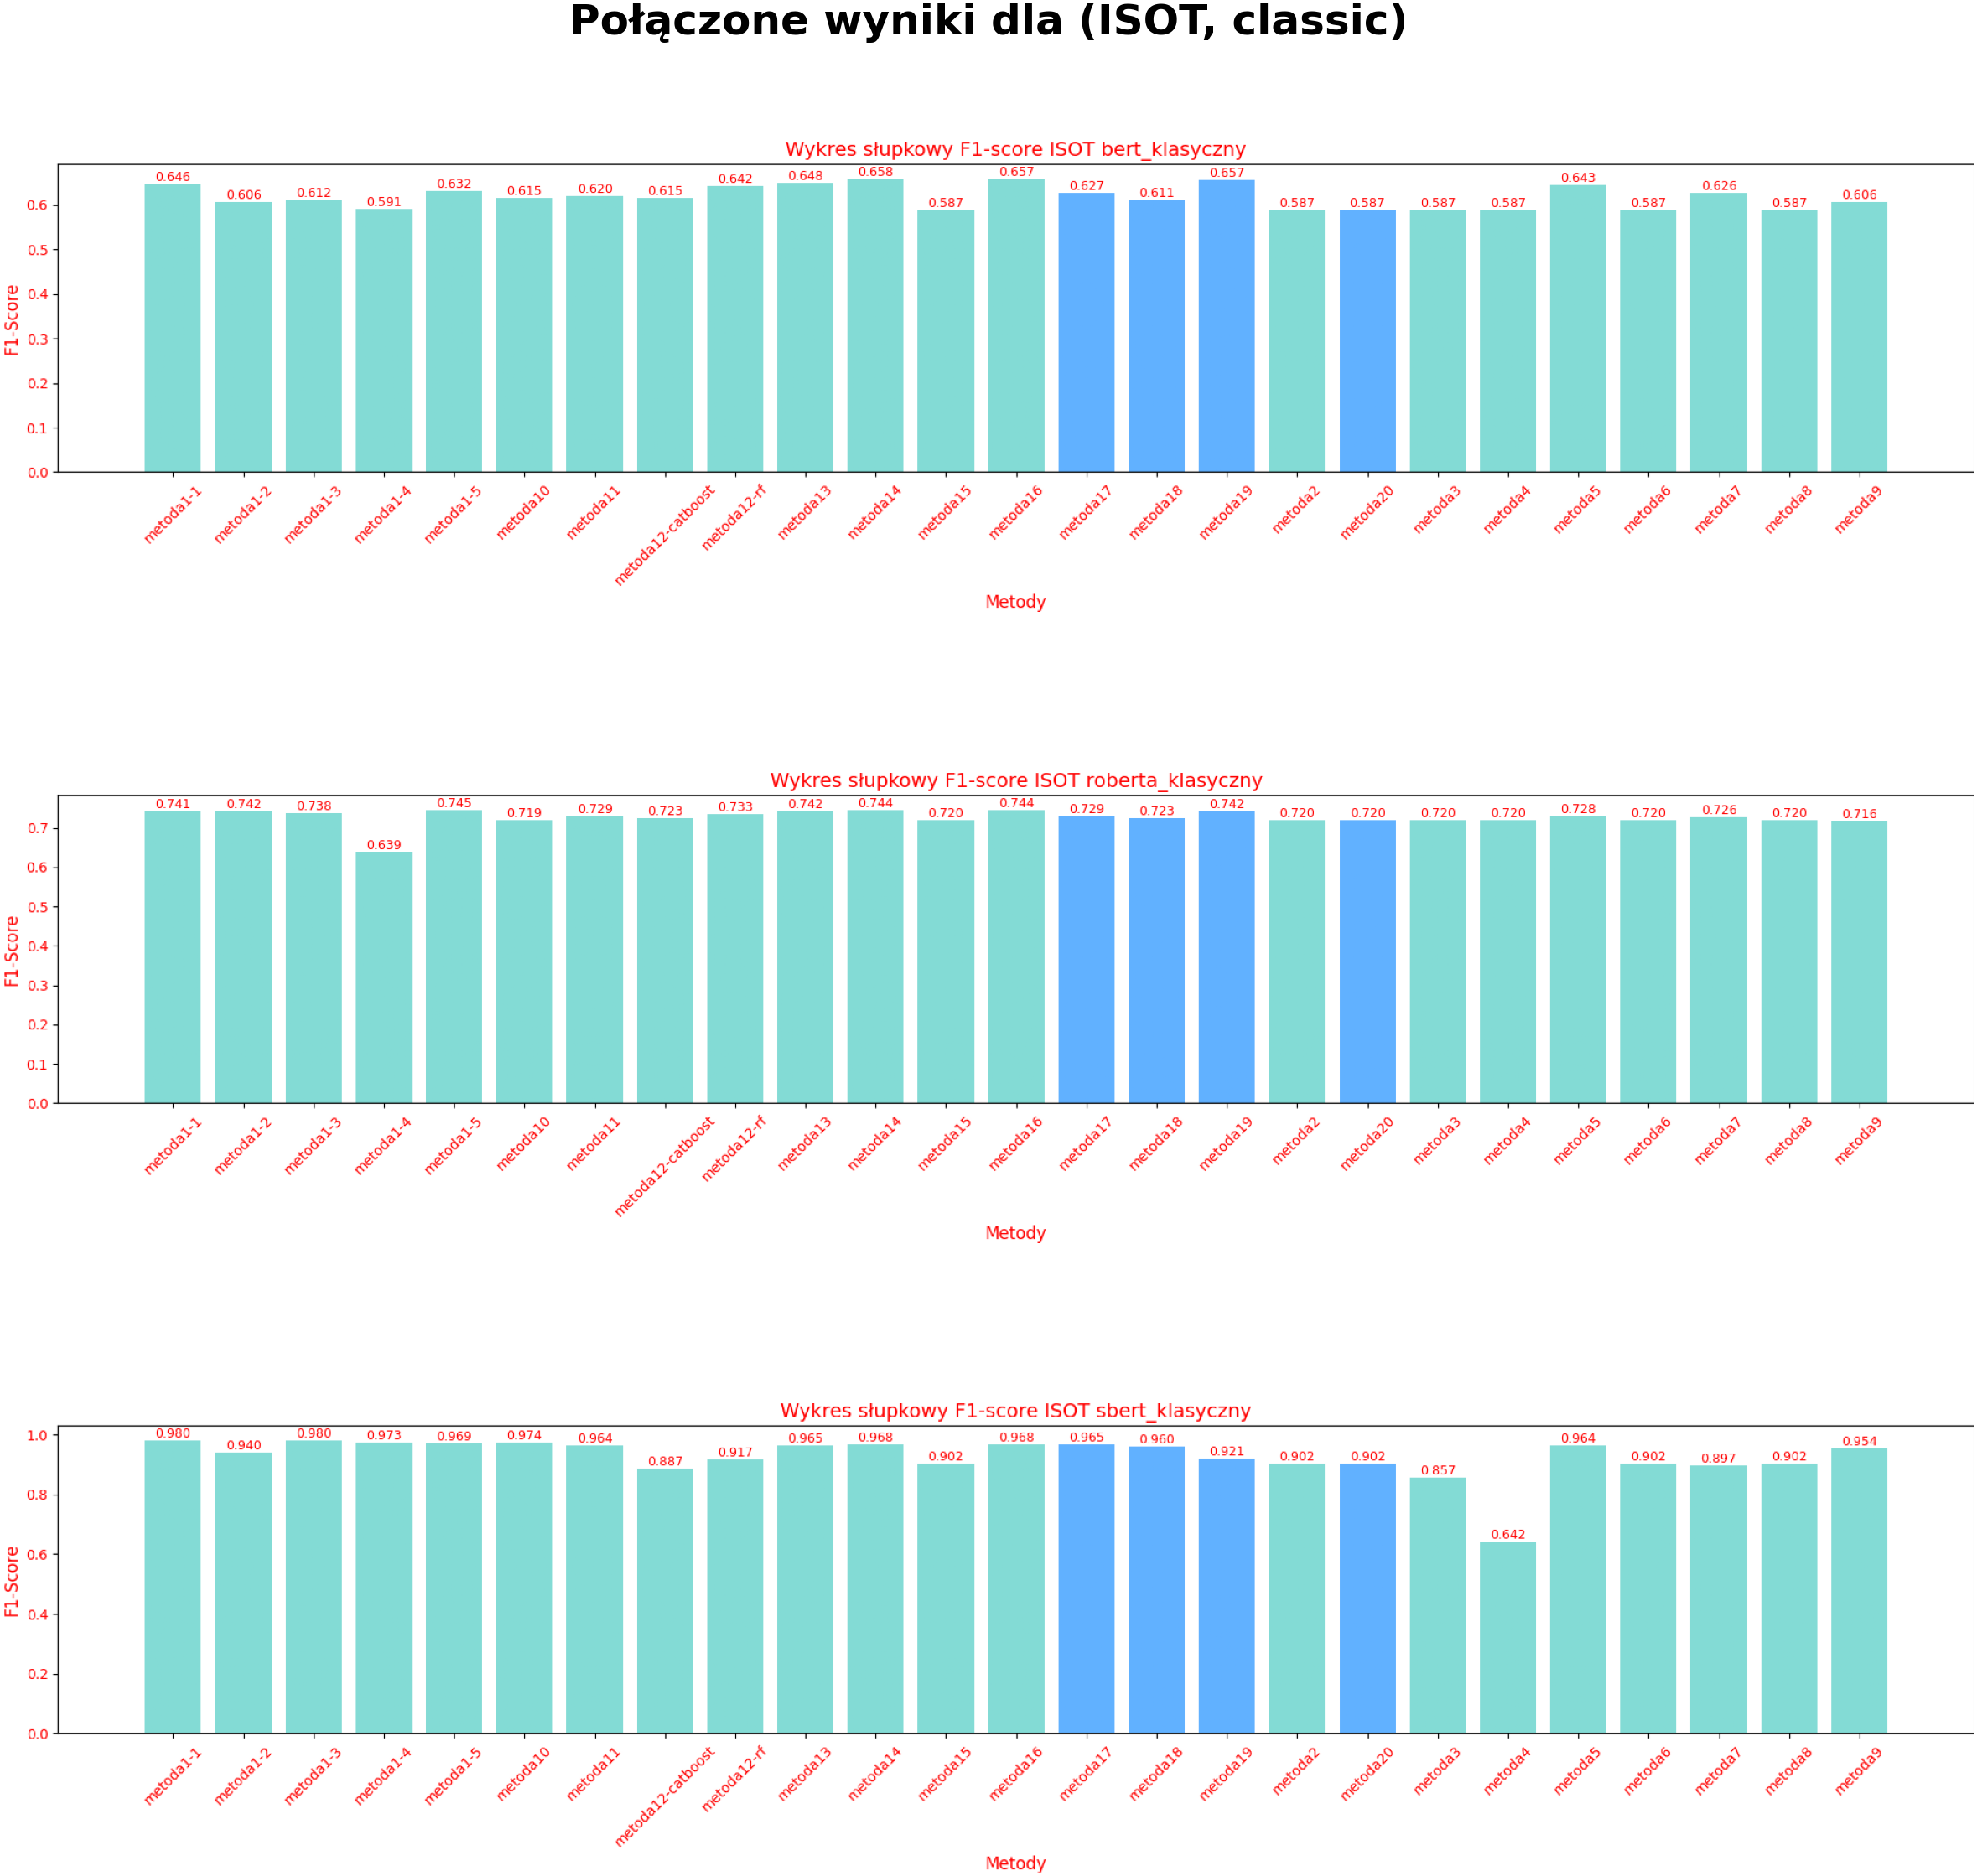
\includegraphics[width=0.99\textwidth]{img/stats/ISOT_classic/ISOT_classic_Combined_F1-Score_bar.png}
	\caption{Histogram rozkładu \textbf{Wyniku F1 (F1-Score)}.}
	\label{fig:isot_classic_f1}
\end{figure}

\subsubsection{ROC-AUC}
Wykresy słupkowe \textbf{Pola pod krzywą ROC-AUC (ROC-AUC)} \ref{fig:isot_classic_roc} przedstawiają rozkład wartości ROC-AUC dla wszystkich badanych metod. Na podstawie wykresu można sformułować następujące obserwacje:
\begin{itemize}
	\item \textbf{Wykres górny (BERT):}
	      \begin{itemize}
		      \item Najwyższe wartości ROC-AUC osiągnęła autorska metoda \texttt{Metoda19} (model stackingowy). Jej wysoka skuteczność wskazuje na to, że ten model jest w stanie efektywnie wykorzystać bogate i złożone cechy generowane przez model BERT, osiągając doskonałą zdolność rozróżniania klas.
		      \item Najniższe wyniki odnotowano dla \texttt{Metoda15}, \texttt{Metoda2}, \texttt{Metoda3}, \texttt{Metoda4}, \texttt{Metoda8} oraz autorskiej \texttt{Metoda20}. Niska wartość ROC-AUC dla tych metod może świadczyć o niedostatecznej optymalizacji ich hiperparametrów dla embeddingów BERT, co skutkuje słabą zdolnością rozróżniania klas.
	      \end{itemize}

	\item \textbf{Wykres środkowy (RoBERTa):}
	      \begin{itemize}
		      \item Najlepsze rezultaty uzyskała autorska metoda \texttt{Metoda19}. Jej dominacja w tej kategorii sugeruje, że ta metoda jest w stanie efektywnie wykorzystać embeddingi RoBERTa, osiągając doskonałą zdolność rozróżniania klas.
		      \item Najsłabsze wyniki wykazały \texttt{Metoda12-rf} (algorytm Random Forest) oraz autorska \texttt{Metoda17} (zaawansowany VotingClassifier). Niska wartość ROC-AUC dla tych metod może wskazywać na ich trudności w generalizacji dla embeddingów RoBERTa.
	      \end{itemize}

	\item \textbf{Wykres dolny (SBERT):}
	      \begin{itemize}
		      \item Najlepsze wartości ROC-AUC osiągnęły praktycznie wszystkie metody. Ten wynik jest wyjątkowy i sugeruje, że embeddingi SBERT są informatywne i "łatwe" do klasyfikacji w kontekście klasycznego uczenia z SBERT, pozwalając większości algorytmów na osiągnięcie doskonałej zdolności rozróżniania klas.
		      \item Najgorsze rezultaty zaobserwowano dla \texttt{Metoda4}. Niska wartość ROC-AUC dla tej metody jest zaskakująca, zwłaszcza w kontekście ogólnej wysokiej wydajności innych metod dla SBERT. Może to sugerować, że mimo jej złożonej struktury, konfiguracja lub proces optymalizacji dla embeddingów SBERT nie były wystarczająco efektywne.
	      \end{itemize}
\end{itemize}

Analiza wykresów słupkowych ROC-AUC dla klasycznego uczenia ujawnia zróżnicowanie w wydajności metod w zależności od typu zastosowanego embeddingu. W przypadku BERT i RoBERTa, dominują autorskie metody stackingowe, takie jak \texttt{Metoda19}, co podkreśla potencjał dobrze skonfigurowanych modeli ensemble w wykorzystywaniu złożonych reprezentacji językowych. Z kolei w przypadku SBERT, obserwujemy niemal uniwersalnie wysokie wyniki ROC-AUC, co sugeruje, że embeddingi te są szczególnie skuteczne i ułatwiają klasyfikację dla większości algorytmów.

Wśród autorskich metod, \texttt{Metoda19} wyróżnia się jako lider dla osadzeń BERT i RoBERTa, osiągając najwyższe ROC-AUC. Z kolei dla SBERT, autorskie metody takie jak \texttt{Metoda17}, \texttt{Metoda18} również osiągają bardzo dobre wyniki, wpisując się w ogólną wysoką wydajność dla tego typu embeddingu. Należy jednak zauważyć, że \texttt{Metoda20} odnotowała słabe wyniki dla BERT, a \texttt{Metoda17} dla RoBERTa. To podkreśla konieczność precyzyjnej optymalizacji metod autorskich pod kątem specyfiki każdego typu embeddingu, aby mogły w pełni wykorzystać swój potencjał w zakresie rozróżniania klas.
\begin{figure}[htbp]
	\centering
	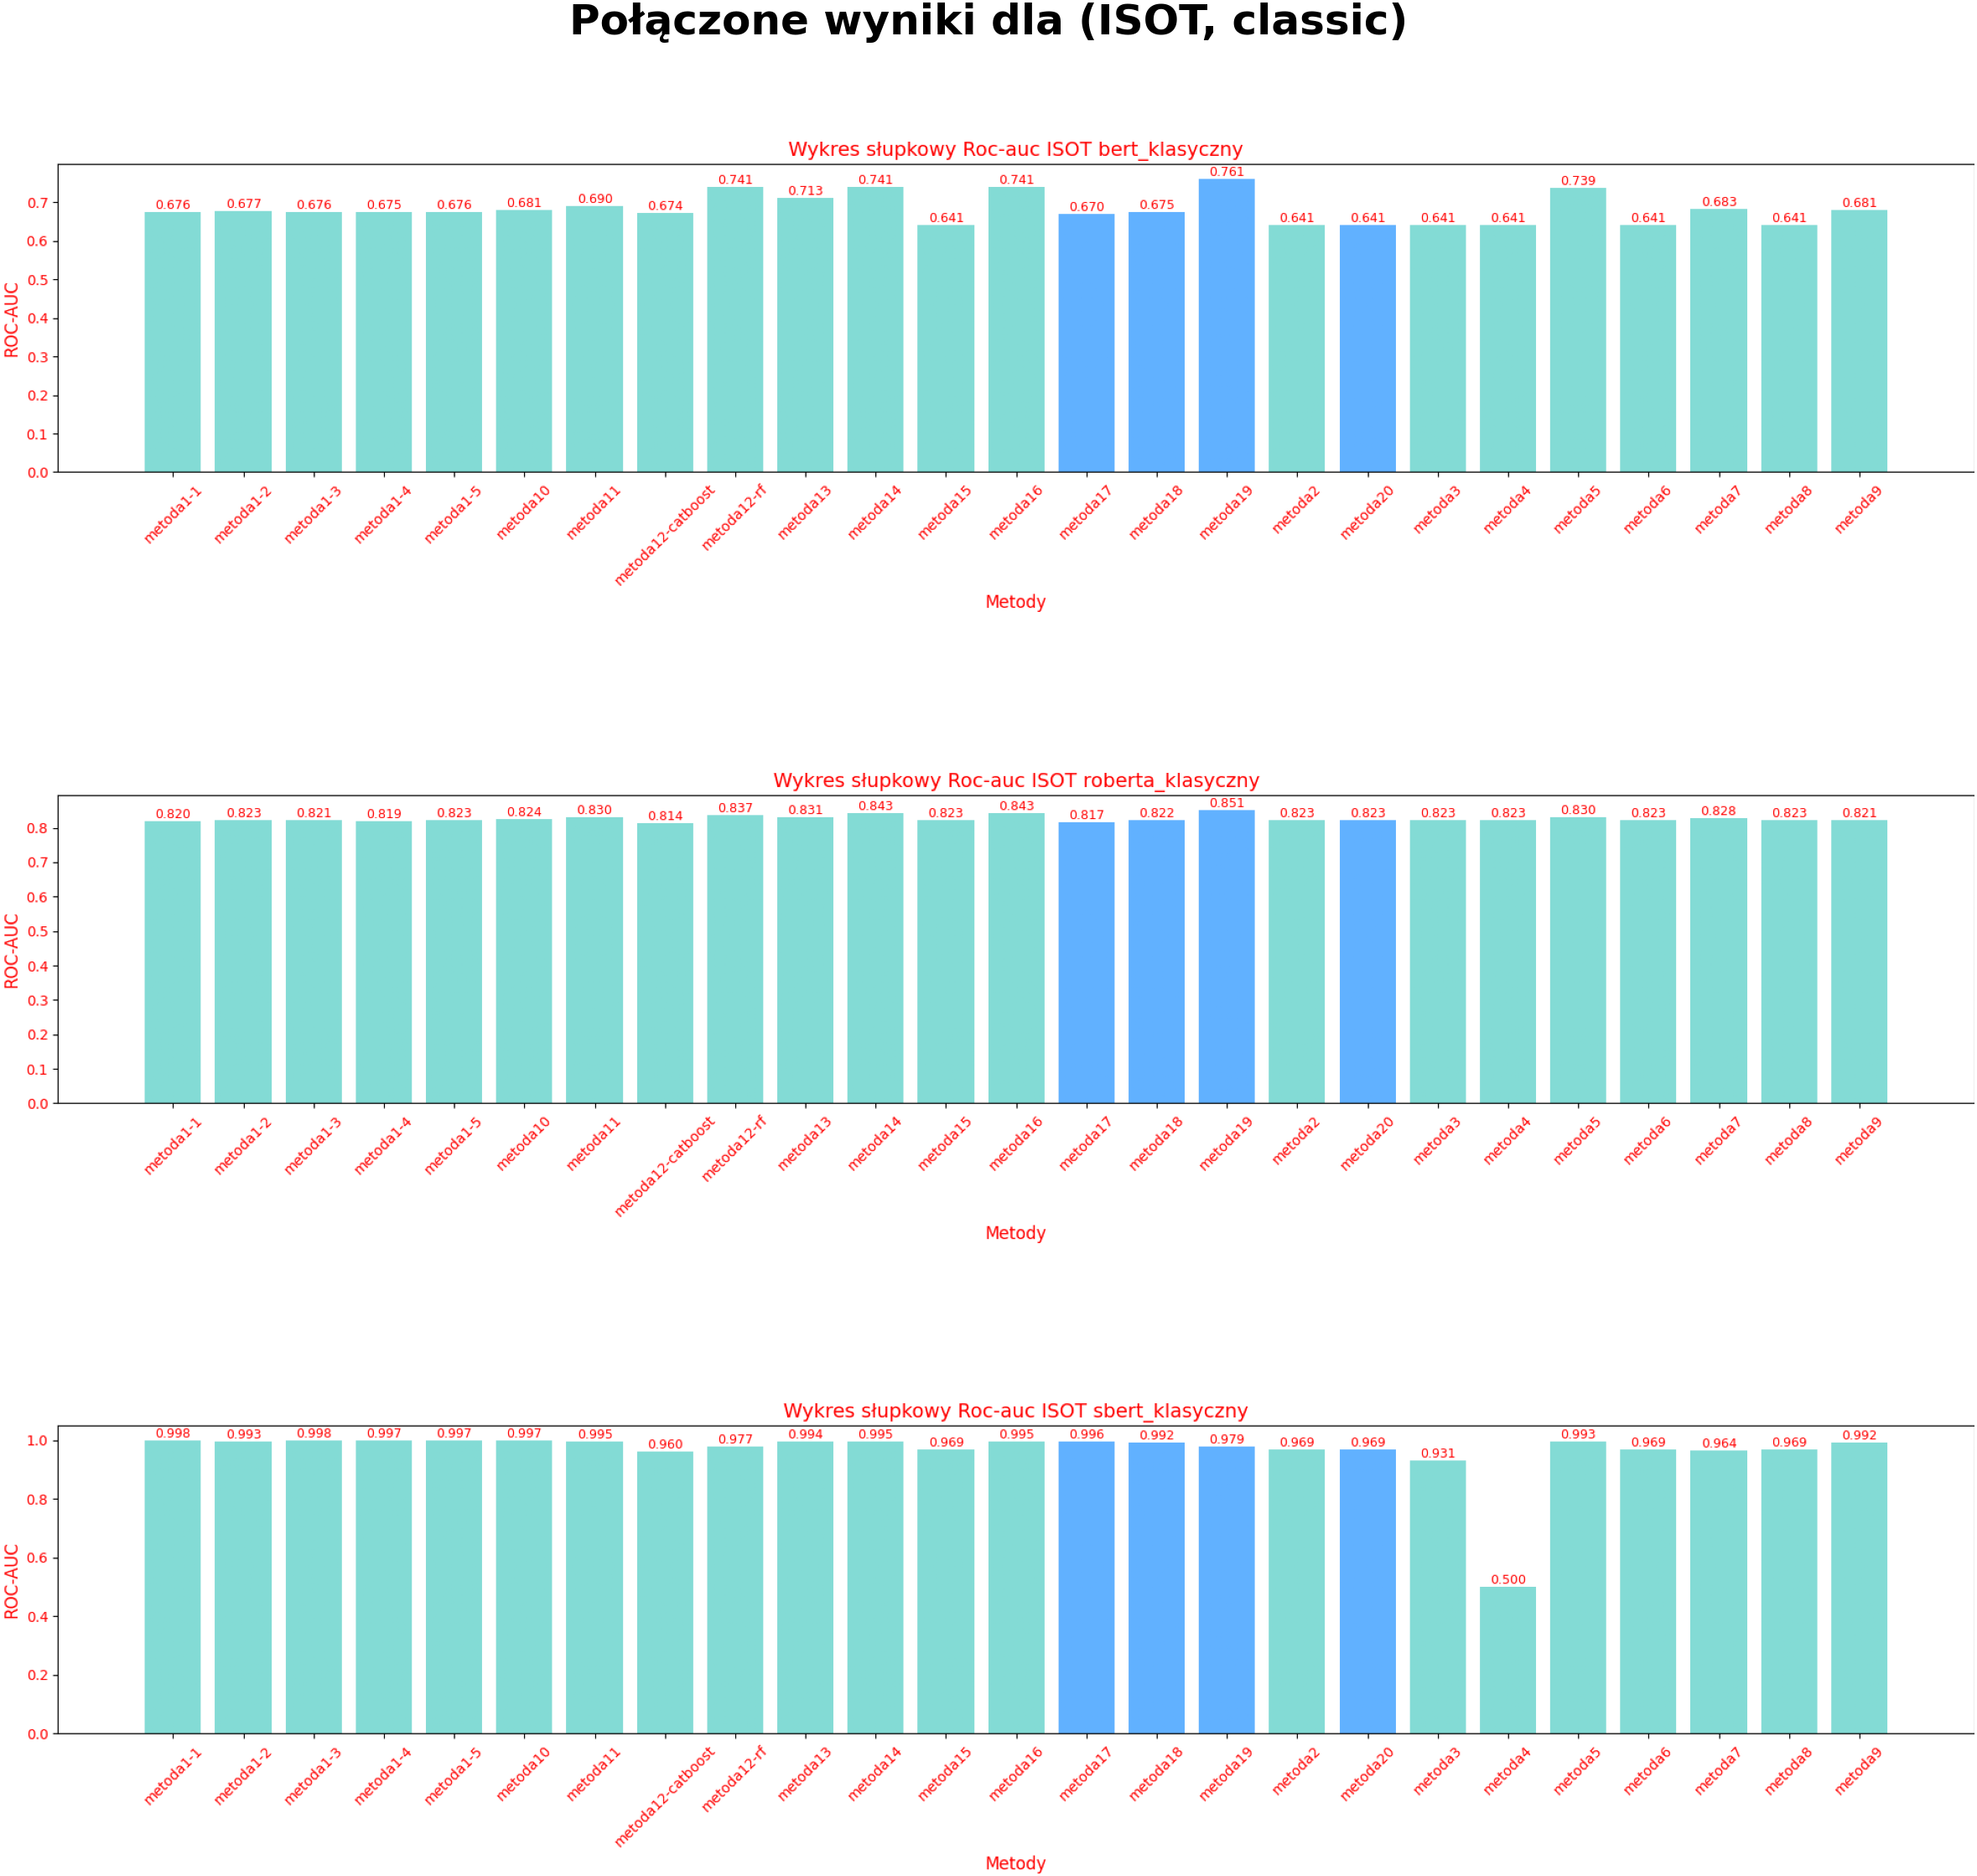
\includegraphics[width=0.99\textwidth]{img/stats/ISOT_classic/ISOT_classic_Combined_ROC-AUC_bar.png}
	\caption{Histogram rozkładu \textbf{Pola pod krzywą ROC-AUC (ROC-AUC)}.}
	\label{fig:isot_classic_roc}
\end{figure}

\subsubsection{Czas wykonania}
Wykres liniowy \textbf{Czasu wykonania (Execution Time)} \ref{fig:isot_classic_prcurve} przedstawia porównanie czasu potrzebnego na wykonanie predykcji przez poszczególne metody dla różnych embeddingów językowych. Na podstawie wykresów można sformułować następujące obserwacje dotyczące efektywności czasowej oraz przyczyn zróżnicowania wyników, z uwzględnieniem zmienności wydajności metod w porównaniu do wcześniejszych eksperymentów:

\begin{itemize}
	\item \textbf{Wykres górny (BERT):}
	      \begin{itemize}
		      \item Najwięcej czasu zajęły metody \texttt{Metoda1} oraz \texttt{Metoda9} – powyżej 8 sekund. \texttt{Metoda1}, będąca ensemble pięciu głębokich sieci neuronowych trenowanych przez 20 epok, jest czasochłonna z powodu wielokrotnego trenowania modeli na rozbudowanych embeddingach BERT (768 wymiarów). \texttt{Metoda9} wymaga intensywnych obliczeń z powodu iteracyjnych algorytmów ensemble, szczególnie Bagging i AdaBoost, oraz kosztownego KNN na dużych danych BERT. W porównaniu do wcześniejszych eksperymentów, \texttt{Metoda1} i \texttt{Metoda9} pozostają konsekwentnie czasochłonne, co potwierdza ich wysoką złożoność obliczeniową.
		      \item Najkrótszy czas wykonania miały \texttt{Metoda10} oraz autorska \texttt{Metoda18} – mniej niż 5 sekund. \texttt{Metoda18}, będąca modelem stackingowym z Gradient Boosting i CatBoost oraz meta-modelem regresji logistycznej, osiąga wysoką efektywność dzięki braku balansowania klas i małej liczbie meta-cech.
	      \end{itemize}

	\item \textbf{Wykres środkowy (RoBERTa):}
	      \begin{itemize}
		      \item Najwięcej czasu zajęły metody \texttt{Metoda3}, \texttt{Metoda4}, \texttt{Metoda6}, \texttt{Metoda8}, \texttt{Metoda15} oraz autorska \texttt{Metoda20} – powyżej 80 sekund. \texttt{Metoda4}, łącząca Bi-LSTM, CNN i MLP, jest czasochłonna z powodu złożonych warstw sekwencyjnych, szczególnie dla rozbudowanych embeddingów RoBERTa (768 wymiarów). \texttt{Metoda20} wymaga więcej czasu niż wcześniej (poniżej 1 sekundy dla BERT), co może wynikać z większej liczby próbek RoBERTa w tym eksperymencie. \texttt{Metoda3}, \texttt{Metoda6}, \texttt{Metoda8} i \texttt{Metoda15} wykorzystują złożone modele.
		      \item Najkrótszy czas wykonania miały \texttt{Metoda10} oraz \texttt{Metoda18} – mniej niż 5 sekund, podobnie jak dla \texttt{BERT}.
	      \end{itemize}

	\item \textbf{Wykres dolny (SBERT):}
	      \begin{itemize}
		      \item Najdłuższy czas działania osiągnęły metody \texttt{Metoda3} oraz \texttt{Metoda16} – około 1200 sekund. \texttt{Metoda3}, wcześniej szybka (poniżej 1 sekundy dla BERT i RoBERTa), teraz jest wyjątkowo czasochłonna, co wynika z zastosowania bardzo złożonego modelu na sporych embeddingach SBERT. \texttt{Metoda16} wykorzystuje zaawansowany model, przykładowo z intensywnymi operacjami na cechach, co prowadzi do ekstremalnie długiego czasu obliczeń. Drastyczny wzrost czasu \texttt{Metoda3} w porównaniu do wcześniejszych eksperymentów sugeruje, że dane SBERT w tym eksperymencie mogły być liczniejsze lub bardziej złożone, z większą liczbą próbek lub wyższą wymiarowością.
		      \item Najkrótszy czas uzyskano dla \texttt{Metoda17} oraz \texttt{Metoda7} – około 20 sekund. \texttt{Metoda17} jest zoptymalizowana poprzez regresję logistyczną, dzięki czemu jest znacznie szybsza niż wcześniej (10–60 sekund dla BERT i RoBERTa), co wynika z bardziej zoptymalizowanej konfiguracji hiperparametrów dla \texttt{SBERT}.
	      \end{itemize}
\end{itemize}

Analiza wykresów czasu wykonania pokazuje, że efektywność czasowa metod zależy od ich architektury, specyfiki embeddingów oraz charakterystyki danych w danym eksperymencie. Złożone modele, takie jak \texttt{Metoda1}, \texttt{Metoda3}, \texttt{Metoda4}, \texttt{Metoda9} czy \texttt{Metoda20}, są czasochłonne z powodu głębokich sieci, iteracyjnych algorytmów ensemble lub dużej liczby próbek, szczególnie dla RoBERTa i SBERT. \texttt{Metoda3} i \texttt{Metoda20} wykazują znaczące pogorszenie efektywności w porównaniu do wcześniejszych eksperymentów, co sugeruje wpływ bardziej złożonych danych. Z kolei \texttt{Metoda17} poprawiła swoją wydajność dla SBERT, co może wynikać z lepszej optymalizacji lub mniejszej liczby próbek. Prostsze metody, takie jak \texttt{Metoda10}, \texttt{Metoda18} czy \texttt{Metoda7}, osiągają krótsze czasy dzięki zoptymalizowanym modelom i efektywnemu wykorzystaniu cech, szczególnie dla SBERT. Zróżnicowanie czasów wykonania podkreśla konieczność dopasowania architektury modelu i optymalizacji hiperparametrów do specyfiki danych i typu embeddingu.
\begin{figure}[H]
	\centering
	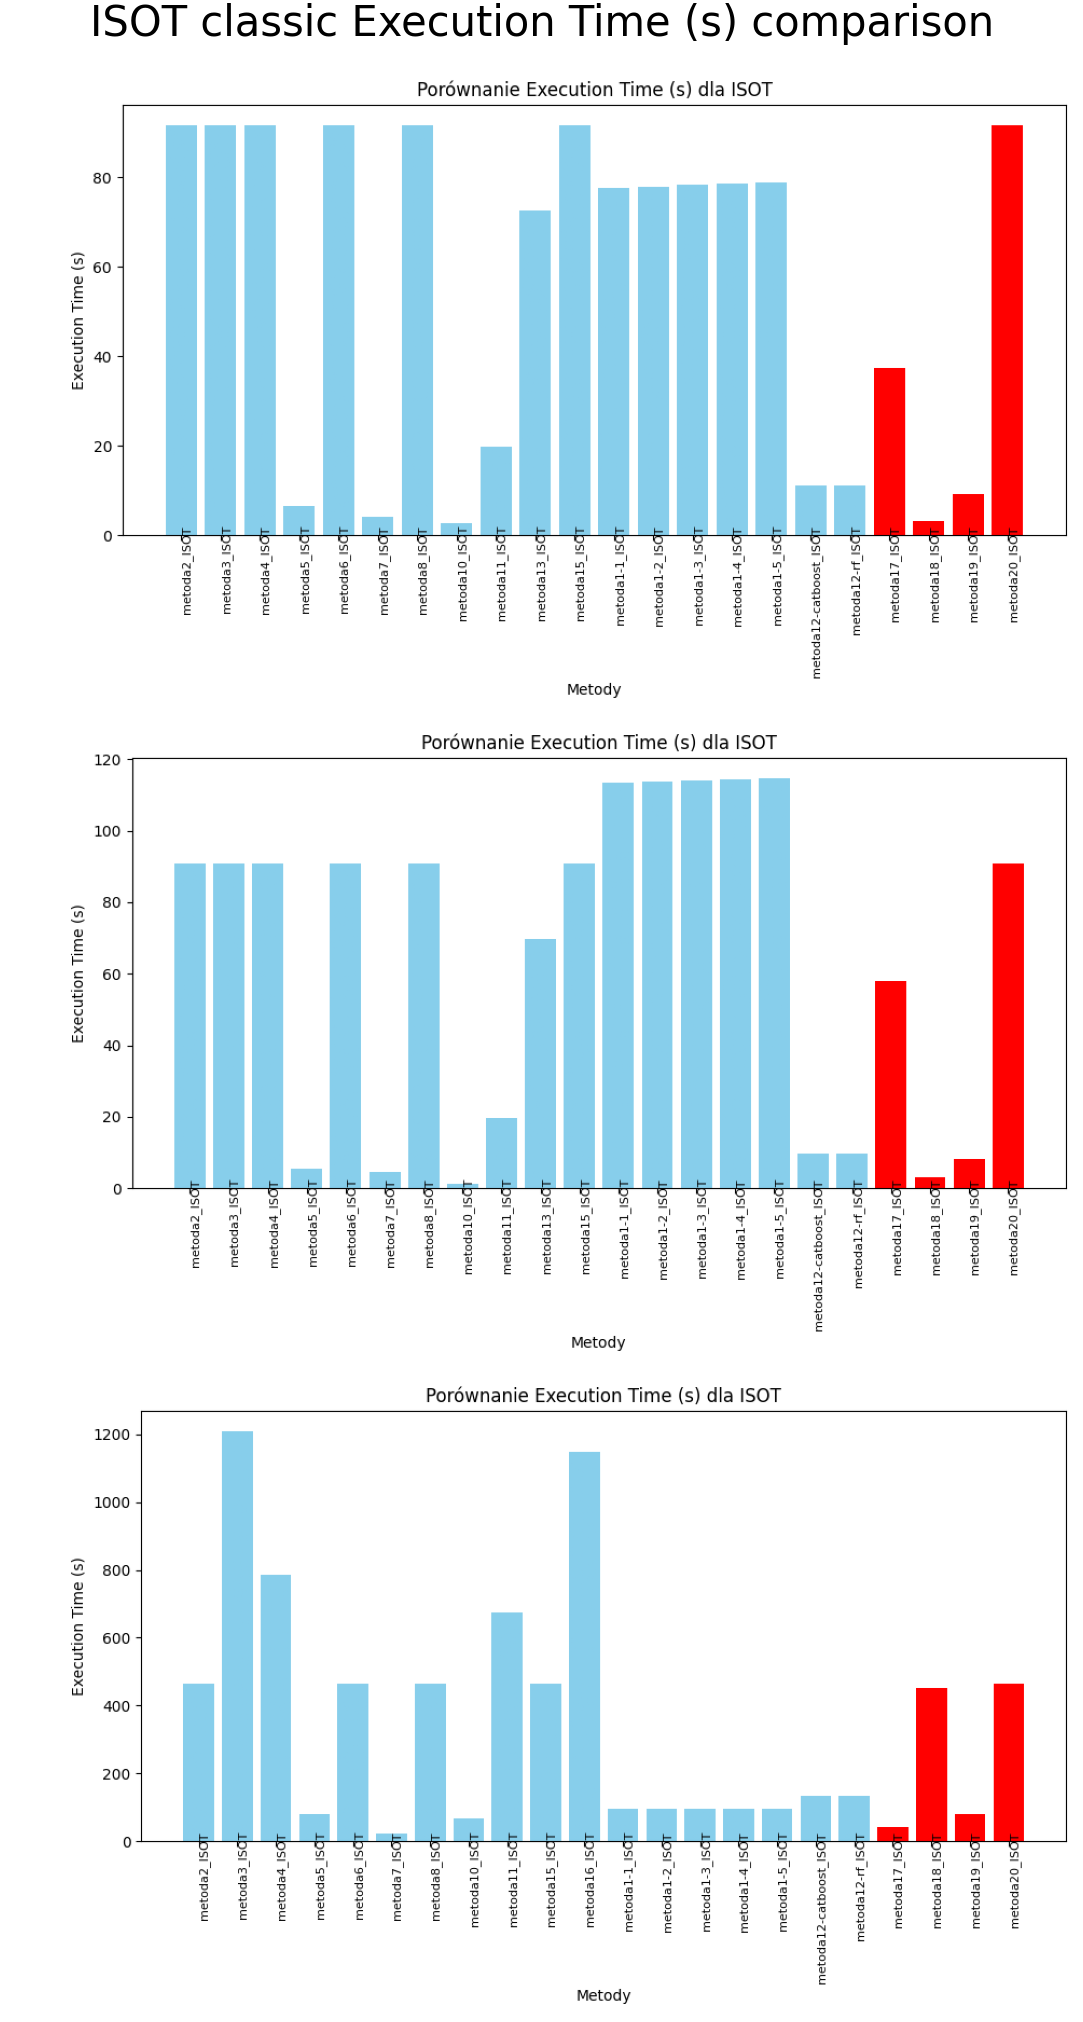
\includegraphics[width=0.99\textwidth]{img/stats/ISOT_classic/ISOT_classic_Execution Time (s)_comparison.png}
	\caption{\textbf{Czas wykonania (Execution Time)} w sekundach.}
	\label{fig:isot_classic_prcurve}
\end{figure}

\subsection{Wyniki w trybie few-shot}
W trybie \textbf{few-shot} dla datasetu \textbf{ISOT}. Poniżej przedstawiono szczegółowy opis wyników w formie histogramów, które ilustrują rozkłady kluczowych metryk, oraz wykresu liniowego czasu wykonania eksperymentów.

\subsubsection{Accuracy}
Wykresy słupkowe \textbf{Dokładności (Accuracy)} \ref{fig:isot_few_shot_accuracy} pokazuje rozkład wartości dokładności dla wszystkich metod. Analizując podany wykres słupkowy można zauważyć następujące rozkłady wyników:

\begin{itemize}
	\item \textbf{Wykres górny (BERT):}
	      \begin{itemize}
		      \item Najlepsze wyniki należą do grupy metod \texttt{Metoda12}, \texttt{Metoda9}, \texttt{Metoda13} oraz autorskiej \texttt{Metoda18}. Ich wysoka dokładność wskazuje na skuteczne wykorzystanie bogatych cech generowanych przez model BERT, co przekłada się na precyzyjną klasyfikację w scenariuszu few-shot.
		      \item Najgorsze wyniki odnotowano dla \texttt{Metoda16} (model zespołowy stacking z meta-klasyfikatorem). Niska dokładność tej metody może świadczyć o trudnościach w efektywnym dopasowaniu do danych z embeddingów BERT, lub o tym, że jej konfiguracja nie jest optymalna dla tego typu zadania few-shot.
	      \end{itemize}

	\item \textbf{Wykres środkowy (RoBERTa):}
	      \begin{itemize}
		      \item Najlepsze wyniki należą do \texttt{Metoda10}, \texttt{Metoda16} oraz autorskiej \texttt{Metoda19}. Wysoka skuteczność tych metod sugeruje, że embeddingi RoBERTa są dobrze dopasowane do zaawansowanych technik ensemble, pozwalając na efektywne wykorzystanie złożonych wzorców w danych i osiągnięcie wysokiej dokładności.
		      \item Najgorsze wyniki odnotowano dla autorskiej \texttt{Metoda17} (zaawansowany VotingClassifier) i \texttt{Metoda1-2} (indywidualna instancja sieci neuronowej). Niska dokładność dla tych metod może wskazywać na ich trudności w generalizacji dla embeddingów RoBERTa, lub na to, że ich konfiguracja jest suboptymalna dla danych w scenariuszu few-shot.
	      \end{itemize}

	\item \textbf{Wykres dolny (SBERT):}
	      \begin{itemize}
		      \item Najlepsze wyniki należą do praktycznie wszystkich metod. Ten wynik jest wyjątkowy i sugeruje, że embeddingi SBERT są maksymalnie informatywne i "łatwe" do klasyfikacji w kontekście few-shot, pozwalając większości algorytmów na osiągnięcie wysokiej dokładności.
		      \item Najgorsze wyniki odnotowano dla \texttt{Metoda4}. Przypominam, że architektura \texttt{Metoda4} jest oparta na zespole sieci Bi-LSTM, CNN i MLP. Niska dokładność tej metody jest zaskakująca, zwłaszcza w kontekście ogólnej wysokiej wydajności innych metod dla SBERT.
	      \end{itemize}
\end{itemize}

Analiza wykresów słupkowych dokładności dla few-shot learningu ujawnia zróżnicowanie w wydajności metod w zależności od typu zastosowanego embeddingu. W przypadku BERT, dominują zaawansowane modele ensemble, takie jak stacking (\texttt{Metoda18}, \texttt{Metoda13}), co podkreśla potencjał tych algorytmów w wykorzystywaniu złożonych reprezentacji językowych. Dla RoBERTa, również metody ensemble (\texttt{Metoda16}, \texttt{Metoda19}) wykazują się wysoką dokładnością. Z kolei w przypadku SBERT, obserwujemy niemal uniwersalnie wysokie wyniki dokładności, co sugeruje, że embeddingi te są szczególnie skuteczne i ułatwiają klasyfikację dla większości algorytmów.

Wśród metod autorskich, \texttt{Metoda18} wyróżnia się dla osadzeń BERT, a \texttt{Metoda19} dla RoBERTa, osiągając wysokie wyniki. W przypadku SBERT, autorskie metody takie jak \texttt{Metoda17} i \texttt{Metoda18} również osiągają bardzo dobre rezultaty, wpisując się w ogólną wysoką wydajność dla tego typu embeddingu. Należy jednak zauważyć, że niektóre metody, w tym autorska \texttt{Metoda17} dla RoBERTa oraz \texttt{Metoda4} dla SBERT, odnotowały słabsze wyniki. To podkreśla konieczność precyzyjnej optymalizacji metod pod kątem specyfiki każdego typu embeddingu, aby mogły w pełni wykorzystać swój potencjał.
\begin{figure}[H]
	\centering
	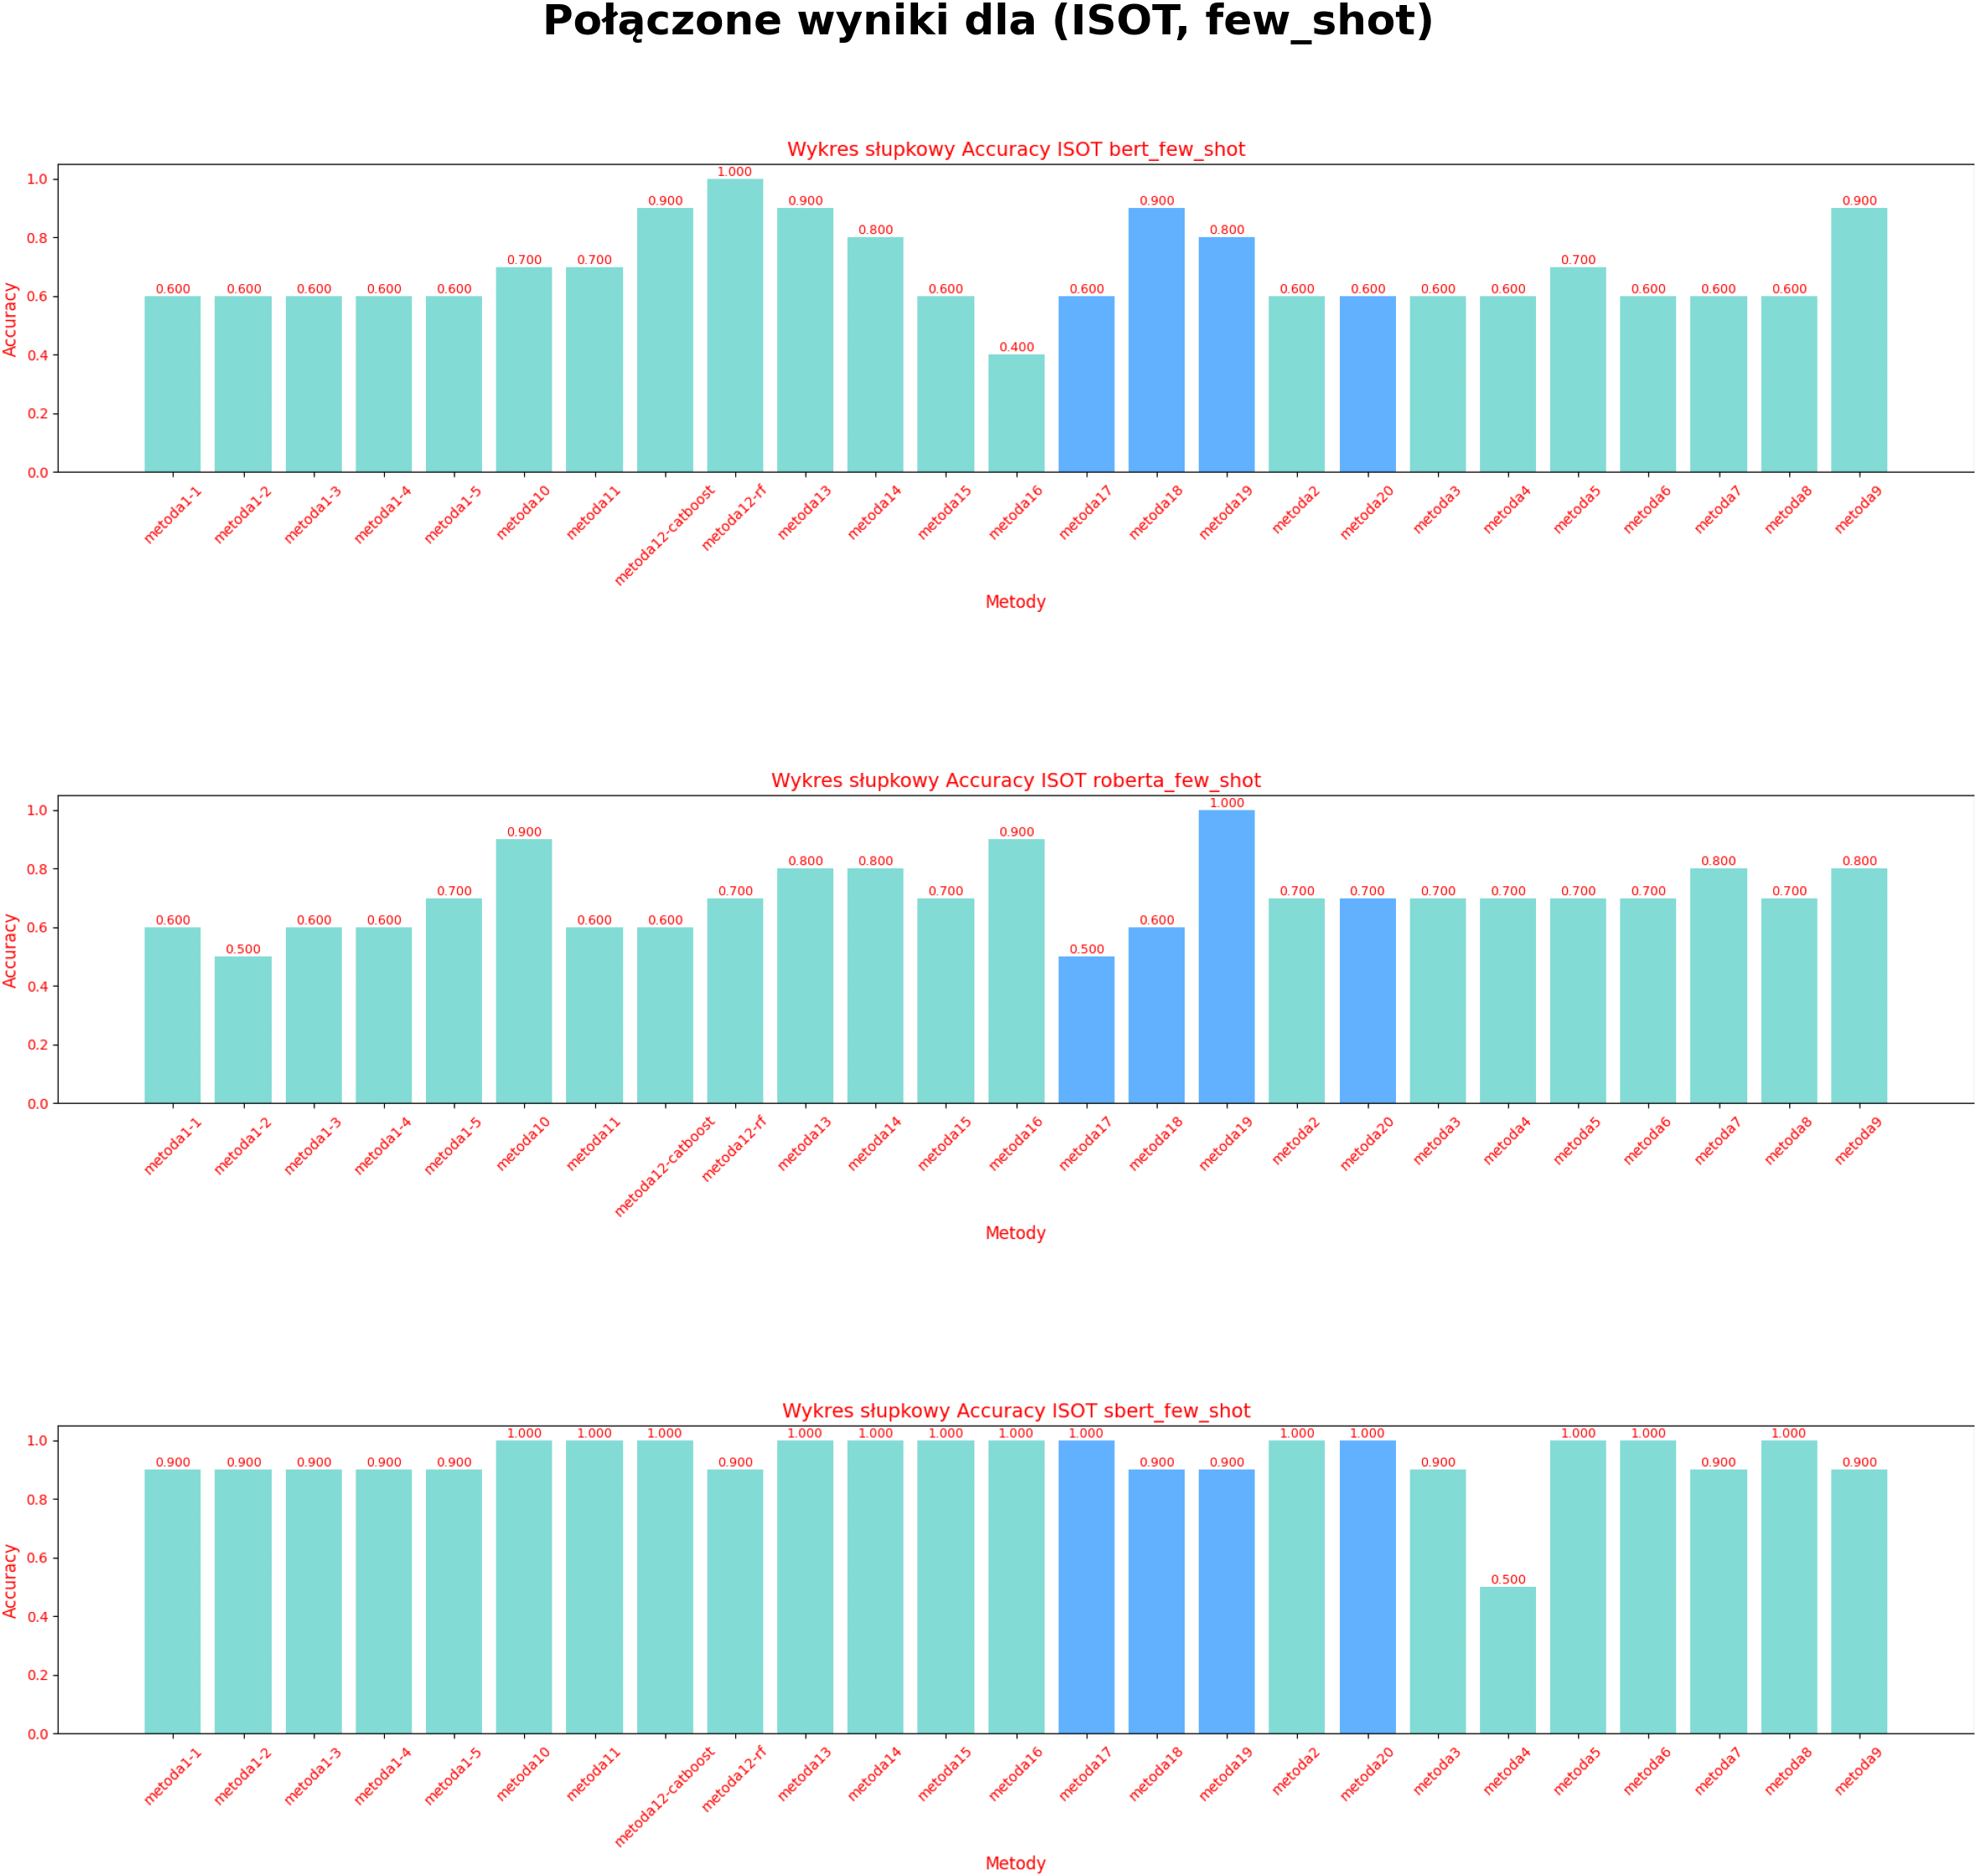
\includegraphics[width=0.99\textwidth]{img/stats/ISOT_few_shot/ISOT_few_shot_Combined_Accuracy_bar_chart.png}
	\caption{Histogram rozkładu \textbf{Dokładności (Accuracy)}.}
	\label{fig:isot_few_shot_accuracy}
\end{figure}

\subsubsection{F1-Score}
Wykresy słupkowe \textbf{Wyniku F1 (F1-Score)} \ref{fig:isot_few_shot_f1} przedstawiają rozkład wartości F1-Score dla wszystkich analizowanych metod. Na podstawie wykresu można sformułować następujące obserwacje:
\begin{itemize}
	\item \textbf{Wykres górny (BERT):}
	      \begin{itemize}
		      \item Najwyższe wartości F1-Score osiągnęły metody takie jak \texttt{Metoda12-rf}, \texttt{Metoda12-catboost}, \texttt{Metoda9}, \texttt{Metoda13} oraz autorska \texttt{Metoda18}. Ich wysoka skuteczność wskazuje na to, że te metody są w stanie efektywnie wykorzystać bogate i złożone cechy generowane przez model BERT, osiągając zbalansowane wyniki między precyzją a recall w scenariuszu few-shot. W przypadku autorskiej \texttt{Metoda18}, będącej modelem stackingowym, sukces prawdopodobnie wynika z jej architektury, która łączy predykcje wielu modeli bazowych, co pozwala na uchwycenie różnorodnych wzorców w danych.
		      \item Najniższe wyniki odnotowano dla \texttt{Metoda16}. Słaby wynik dla tej metody sugeruje, że w kontekście few-shot learningu z embeddingami BERT, nie była ona w stanie odpowiednio zbalansować precyzji i recall. Może to być spowodowane trudnościami w adaptacji jej meta-klasyfikatora: regresji logistycznej w przypadku Metody16 z poprzednich opisów do specyfiki danych BERT.
	      \end{itemize}
	\item \textbf{Wykres środkowy (RoBERTa):}
	      \begin{itemize}
		      \item Najlepsze rezultaty uzyskały metody \texttt{Metoda10}, \texttt{Metoda9}, \texttt{Metoda7}, \texttt{Metoda13}, \texttt{Metoda14}, \texttt{Metoda16} oraz autorska \texttt{Metoda19}. Wysoka skuteczność tej grupy metod świadczy o tym, że embeddingi RoBERTa są bardzo dobrze dopasowane do różnorodnych, zaawansowanych technik klasyfikacji, pozwalając na efektywne wykorzystanie złożonych wzorców w danych i osiągnięcie zbalansowanych wyników. Ich efektywność może wynikać z umiejętności radzenia sobie z zaszumionymi danymi i wyłapywania istotnych zależności. Na przykład, w przypadku autorskiej \texttt{Metoda19}, będącej modelem stackingowym, jej zdolność do integracji różnych perspektyw modeli bazowych mogła być kluczowa dla sukcesu z bogatymi w niuanse embeddingami RoBERTa.
		      \item Najsłabsze wyniki wykazały \texttt{Metoda1-2} oraz autorska \texttt{Metoda17}. Niska wartość F1-Score dla \texttt{Metoda1-2}, będącej indywidualną instancją sieci neuronowej, może wskazywać na to, że jej prosta architektura nie jest wystarczająco złożona, aby efektywnie przetwarzać subtelne zależności w embeddingach RoBERTa w trybie few-shot, co prowadzi do niezbalansowanej precyzji i recall. W przypadku autorskiej \texttt{Metoda17}, która jest zaawansowanym VotingClassifierem, słaby wynik może być spowodowany nieoptymalnym doborem klasyfikatorów bazowych lub wag głosowania dla specyfiki RoBERTa, co uniemożliwiło jej pełne wykorzystanie potencjału ensemble.
	      \end{itemize}
	\item \textbf{Wykres dolny (SBERT):}
	      \begin{itemize}
		      \item Najlepsze wartości F1-Score osiągnęły autorskie metody: \texttt{Metoda20} i \texttt{Metoda17}. Ich wysoka wydajność podkreśla zdolność tych autorskich rozwiązań do efektywnego przetwarzania embeddingów SBERT i osiągania zbalansowanej klasyfikacji, nawet w trudnym scenariuszu few-shot. Sukces tych metod może być związany z ich zdolnością do adaptacji do specyficznych cech reprezentacji SBERT. W przypadku \texttt{Metoda17} (zaawansowany VotingClassifier), jej elastyczność w łączeniu predykcji różnych modeli bazowych mogła pozwolić na uchwycenie różnorodnych aspektów danych SBERT, co przełożyło się na wysoką wartość F1-Score.
		      \item Najgorsze rezultaty zaobserwowano dla \texttt{Metoda4}. Niska wartość F1-Score dla tej metody, pomimo ogólnie dobrych wyników dla SBERT, sugeruje, że w tym konkretnym przypadku mogła ona mieć trudności z optymalizacją. \texttt{Metoda4}, będąca architekturą opartą na zespole sieci Bi-LSTM, CNN i MLP, jest modelem głębokiego uczenia. Jej słabe wyniki mogą wynikać z trudności w trenowaniu tak złożonej architektury na bardzo ograniczonej liczbie przykładów dostępnych w scenariuszu few-shot, co skutkowało niezbalansowaną wydajnością precyzji i recall.
	      \end{itemize}
\end{itemize}
Analiza wykresów słupkowych F1-Score dla few-shot learningu ujawnia zróżnicowanie w wydajności metod w zależności od typu zastosowanego embeddingu. W przypadku BERT i RoBERTa, dominują zaawansowane modele ensemble, takie jak autorskie \texttt{Metoda18} i \texttt{Metoda19}, co podkreśla potencjał tych algorytmów w wykorzystywaniu złożonych reprezentacji językowych. Ich zdolność do łączenia predykcji z wielu modeli bazowych prawdopodobnie przyczynia się do robustności i wysokich wyników. Dla SBERT, również autorskie metody ensemble (\texttt{Metoda20}, \texttt{Metoda17}) wykazują się wysoką wartością F1-Score, co może wynikać z ich elastyczności w adaptacji do unikalnych właściwości embeddingów SBERT.

Należy jednak zauważyć, że niektóre metody, w tym autorska \texttt{Metoda17} dla RoBERTa, odnotowały słabsze wyniki. To podkreśla konieczność precyzyjnej optymalizacji każdej metody pod kątem specyfiki każdego typu embeddingu. Słabe wyniki mogą być efektem niedopasowania modelu do charakterystyki danych, nadmiernego skomplikowania lub zbyt prostej architektury w stosunku do wyzwań few-shot learningu, prowadzącej do niezbalansowanej wydajności.
\begin{figure}[H]
	\centering
	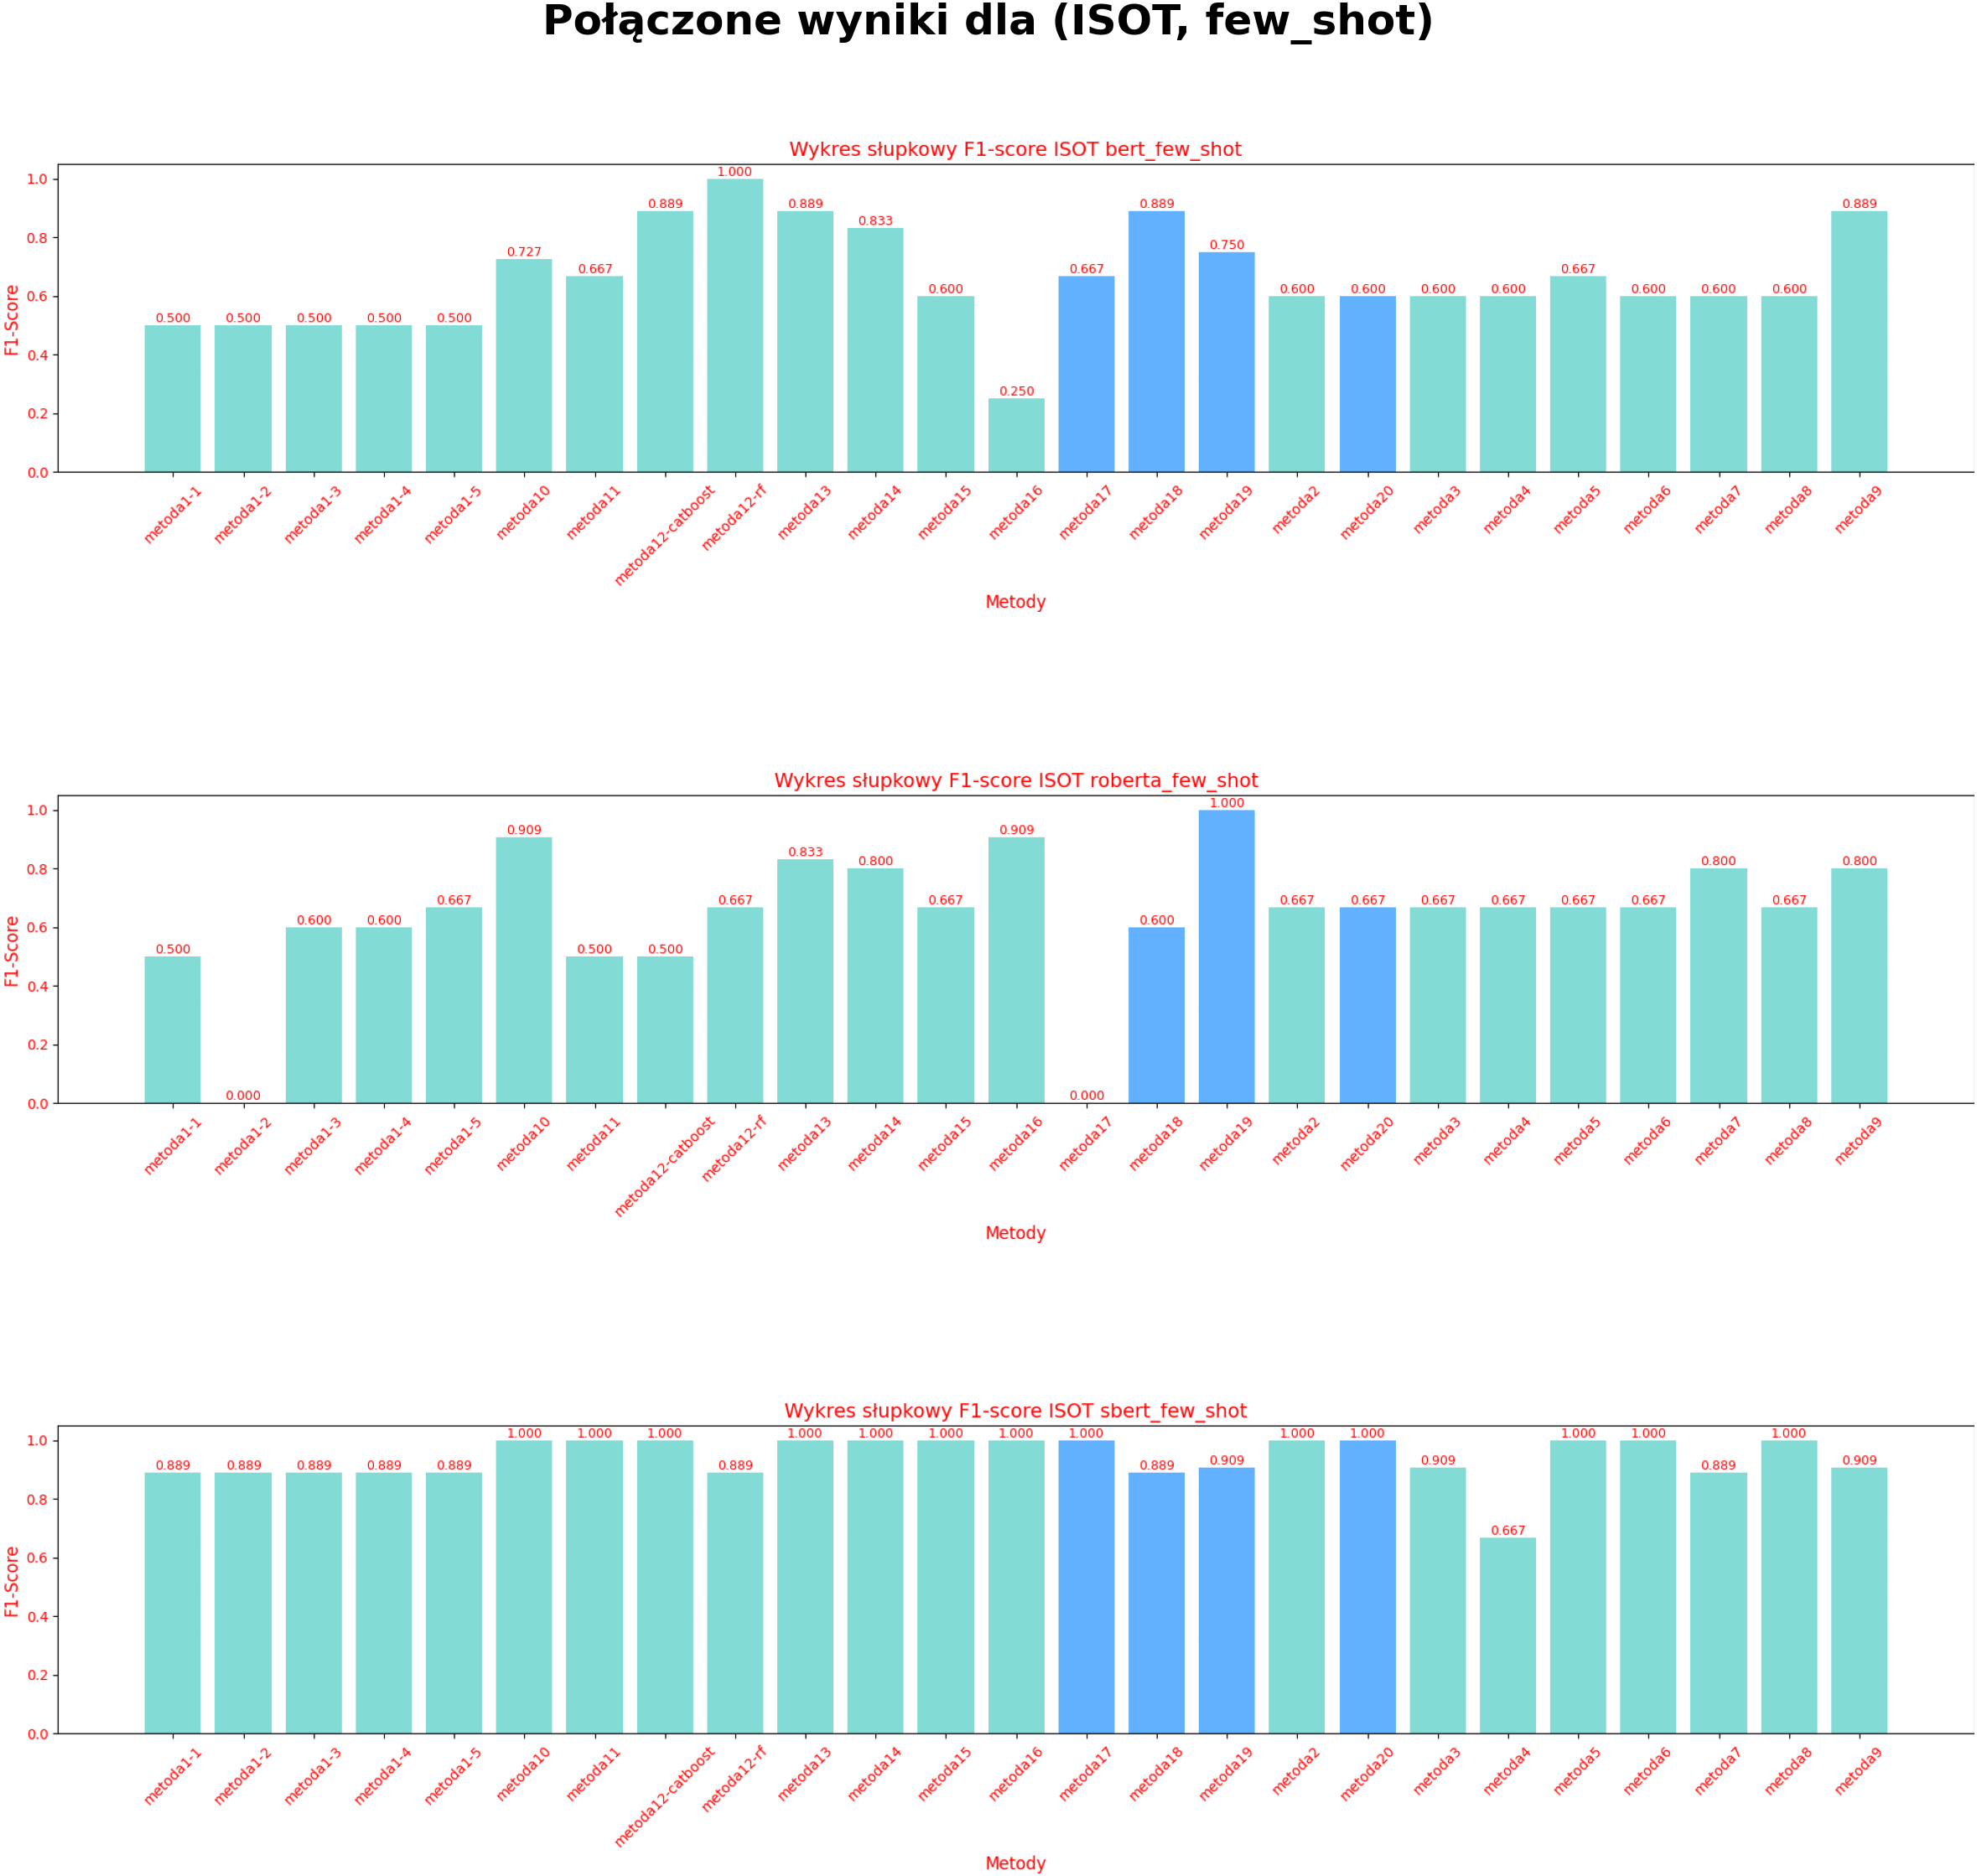
\includegraphics[width=0.99\textwidth]{img/stats/ISOT_few_shot/ISOT_few_shot_Combined_F1-Score_bar.png}
	\caption{Histogram rozkładu \textbf{Wyniku F1 (F1-Score)}.}
	\label{fig:isot_few_shot_f1}
\end{figure}

\subsubsection{ROC-AUC}
Wykresy słupkowe \textbf{Pola pod krzywą ROC-AUC (ROC-AUC)} \ref{fig:isot_few_shot_roc} przedstawia rozkład wartości ROC-AUC dla wszystkich badanych metod. Na podstawie wykresu można sformułować następujące obserwacje:

\begin{itemize}
	\item \textbf{Wykres górny (BERT):}
	      \begin{itemize}
		      \item Najwyższe wartości ROC-AUC osiągnęły metody \texttt{Metoda14} (model zespołowy stacking) oraz \texttt{Metoda12-rf} (oparta na algorytmie Random Forest). Ich wysoka skuteczność w kontekście ROC-AUC świadczy o doskonałej zdolności tych modeli do rozróżniania klas na danych z embeddingów BERT, nawet w scenariuszu few-shot. To wskazuje na ich robustność i zdolność do wyłapywania istotnych wzorców w danych.
		      \item Najniższe wyniki odnotowano dla metody \texttt{Metoda16} (model zespołowy stacking z meta-klasyfikatorem). Słaby wynik dla tej metody sugeruje, że w kontekście few-shot learningu z embeddingami BERT, jej architektura nie była w stanie efektywnie odróżnić klas, co może być spowodowane niedopasowaniem meta-klasyfikatora do charakterystyki danych lub problemami z generalizacją na ograniczonej liczbie przykładów.
	      \end{itemize}

	\item \textbf{Wykres środkowy (RoBERTa):}
	      \begin{itemize}
		      \item Najlepsze rezultaty uzyskały metody \texttt{Metoda14} (model zespołowy stacking), \texttt{Metoda16} (model zespołowy stacking z meta-klasyfikatorem) oraz na dość wysokim poziomie są wyniki dla autorskiej \texttt{Metoda19} (model stackingowy). Wysoka wartość ROC-AUC dla tych metod wskazuje na ich efektywność w przetwarzaniu embeddingów RoBERTa i osiąganiu doskonałej zdolności rozróżniania klas. Modele stackingowe, takie jak \texttt{Metoda19}, mogą czerpać zróżnicowane perspektywy z modeli bazowych, co prowadzi do lepszej ogólnej wydajności.
		      \item Najsłabsze wyniki wykazała autorska \texttt{Metoda17} (zaawansowany VotingClassifier). Niska wartość ROC-AUC dla tej metody, która jest złożonym modelem ensemble, może wskazywać na nieoptymalny dobór klasyfikatorów bazowych lub wag głosowania dla specyfiki embeddingów RoBERTa w trybie few-shot. To uniemożliwiło jej pełne wykorzystanie potencjału ensemble w zakresie rozróżniania klas.
	      \end{itemize}

	\item \textbf{Wykres dolny (SBERT):}
	      \begin{itemize}
		      \item Najlepsze wartości ROC-AUC osiągnęły wszystkie metody. Ten wynik jest wyjątkowy i sugeruje, że embeddingi SBERT są wysoce informatywne i "łatwe" do klasyfikacji w kontekście few-shot, pozwalając większości algorytmów na osiągnięcie niemal perfekcyjnej zdolności rozróżniania klas. Może to wynikać z ich specyficznej architektury, która generuje bardzo wyraźne i łatwo separowalne reprezentacje.
		      \item Najgorsze rezultaty zaobserwowano dla \texttt{Metoda4} (architektura oparta na zespole sieci Bi-LSTM, CNN i MLP). Niska wartość ROC-AUC dla tej metody, pomimo ogólnie doskonałych wyników dla SBERT, sugeruje, że w tym konkretnym przypadku mogła ona mieć trudności z optymalizacją. \texttt{Metoda4} jest modelem głębokiego uczenia, a jej słabe wyniki mogą wynikać z trudności w efektywnym trenowaniu tak złożonej architektury na bardzo ograniczonej liczbie przykładów dostępnych w scenariuszu few-shot. To mogło skutkować niedostateczną zdolnością do rozróżniania klas, pomimo wysokiej jakości danych wejściowych z SBERT.
	      \end{itemize}
\end{itemize}

Analiza wykresów słupkowych ROC-AUC dla few-shot learningu ujawnia zróżnicowanie w wydajności metod w zależności od typu zastosowanego embeddingu. W przypadku BERT i RoBERTa, dominują zaawansowane modele ensemble, takie jak stacking (\texttt{Metoda14}, \texttt{Metoda16}, autorska \texttt{Metoda19}), co podkreśla ich zdolność do efektywnego wykorzystywania złożonych reprezentacji językowych i osiągania wysokiej zdolności rozróżniania klas. Z kolei w przypadku SBERT, obserwujemy niemal uniwersalnie wysokie wyniki ROC-AUC, co sugeruje, że embeddingi te są szczególnie skuteczne i ułatwiają klasyfikację dla większości algorytmów, choć nawet w tym przypadku, bardzo złożone architektury głębokiego uczenia mogą mieć trudności w optymalizacji w scenariuszu few-shot.

Wśród metod autorskich, \texttt{Metoda19} wyróżnia się dla osadzeń RoBERTa, osiągając bardzo wysokie ROC-AUC. Jednakże, \texttt{Metoda17} odnotowała słabsze wyniki dla RoBERTa, a \texttt{Metoda4} dla SBERT. To podkreśla, że nawet zaawansowane metody autorskie wymagają precyzyjnej optymalizacji i dostosowania do specyfiki każdego typu embeddingu oraz wyzwań few-shot learningu, aby mogły w pełni wykorzystać swój potencjał w zakresie rozróżniania klas.
\begin{figure}[H]
	\centering
	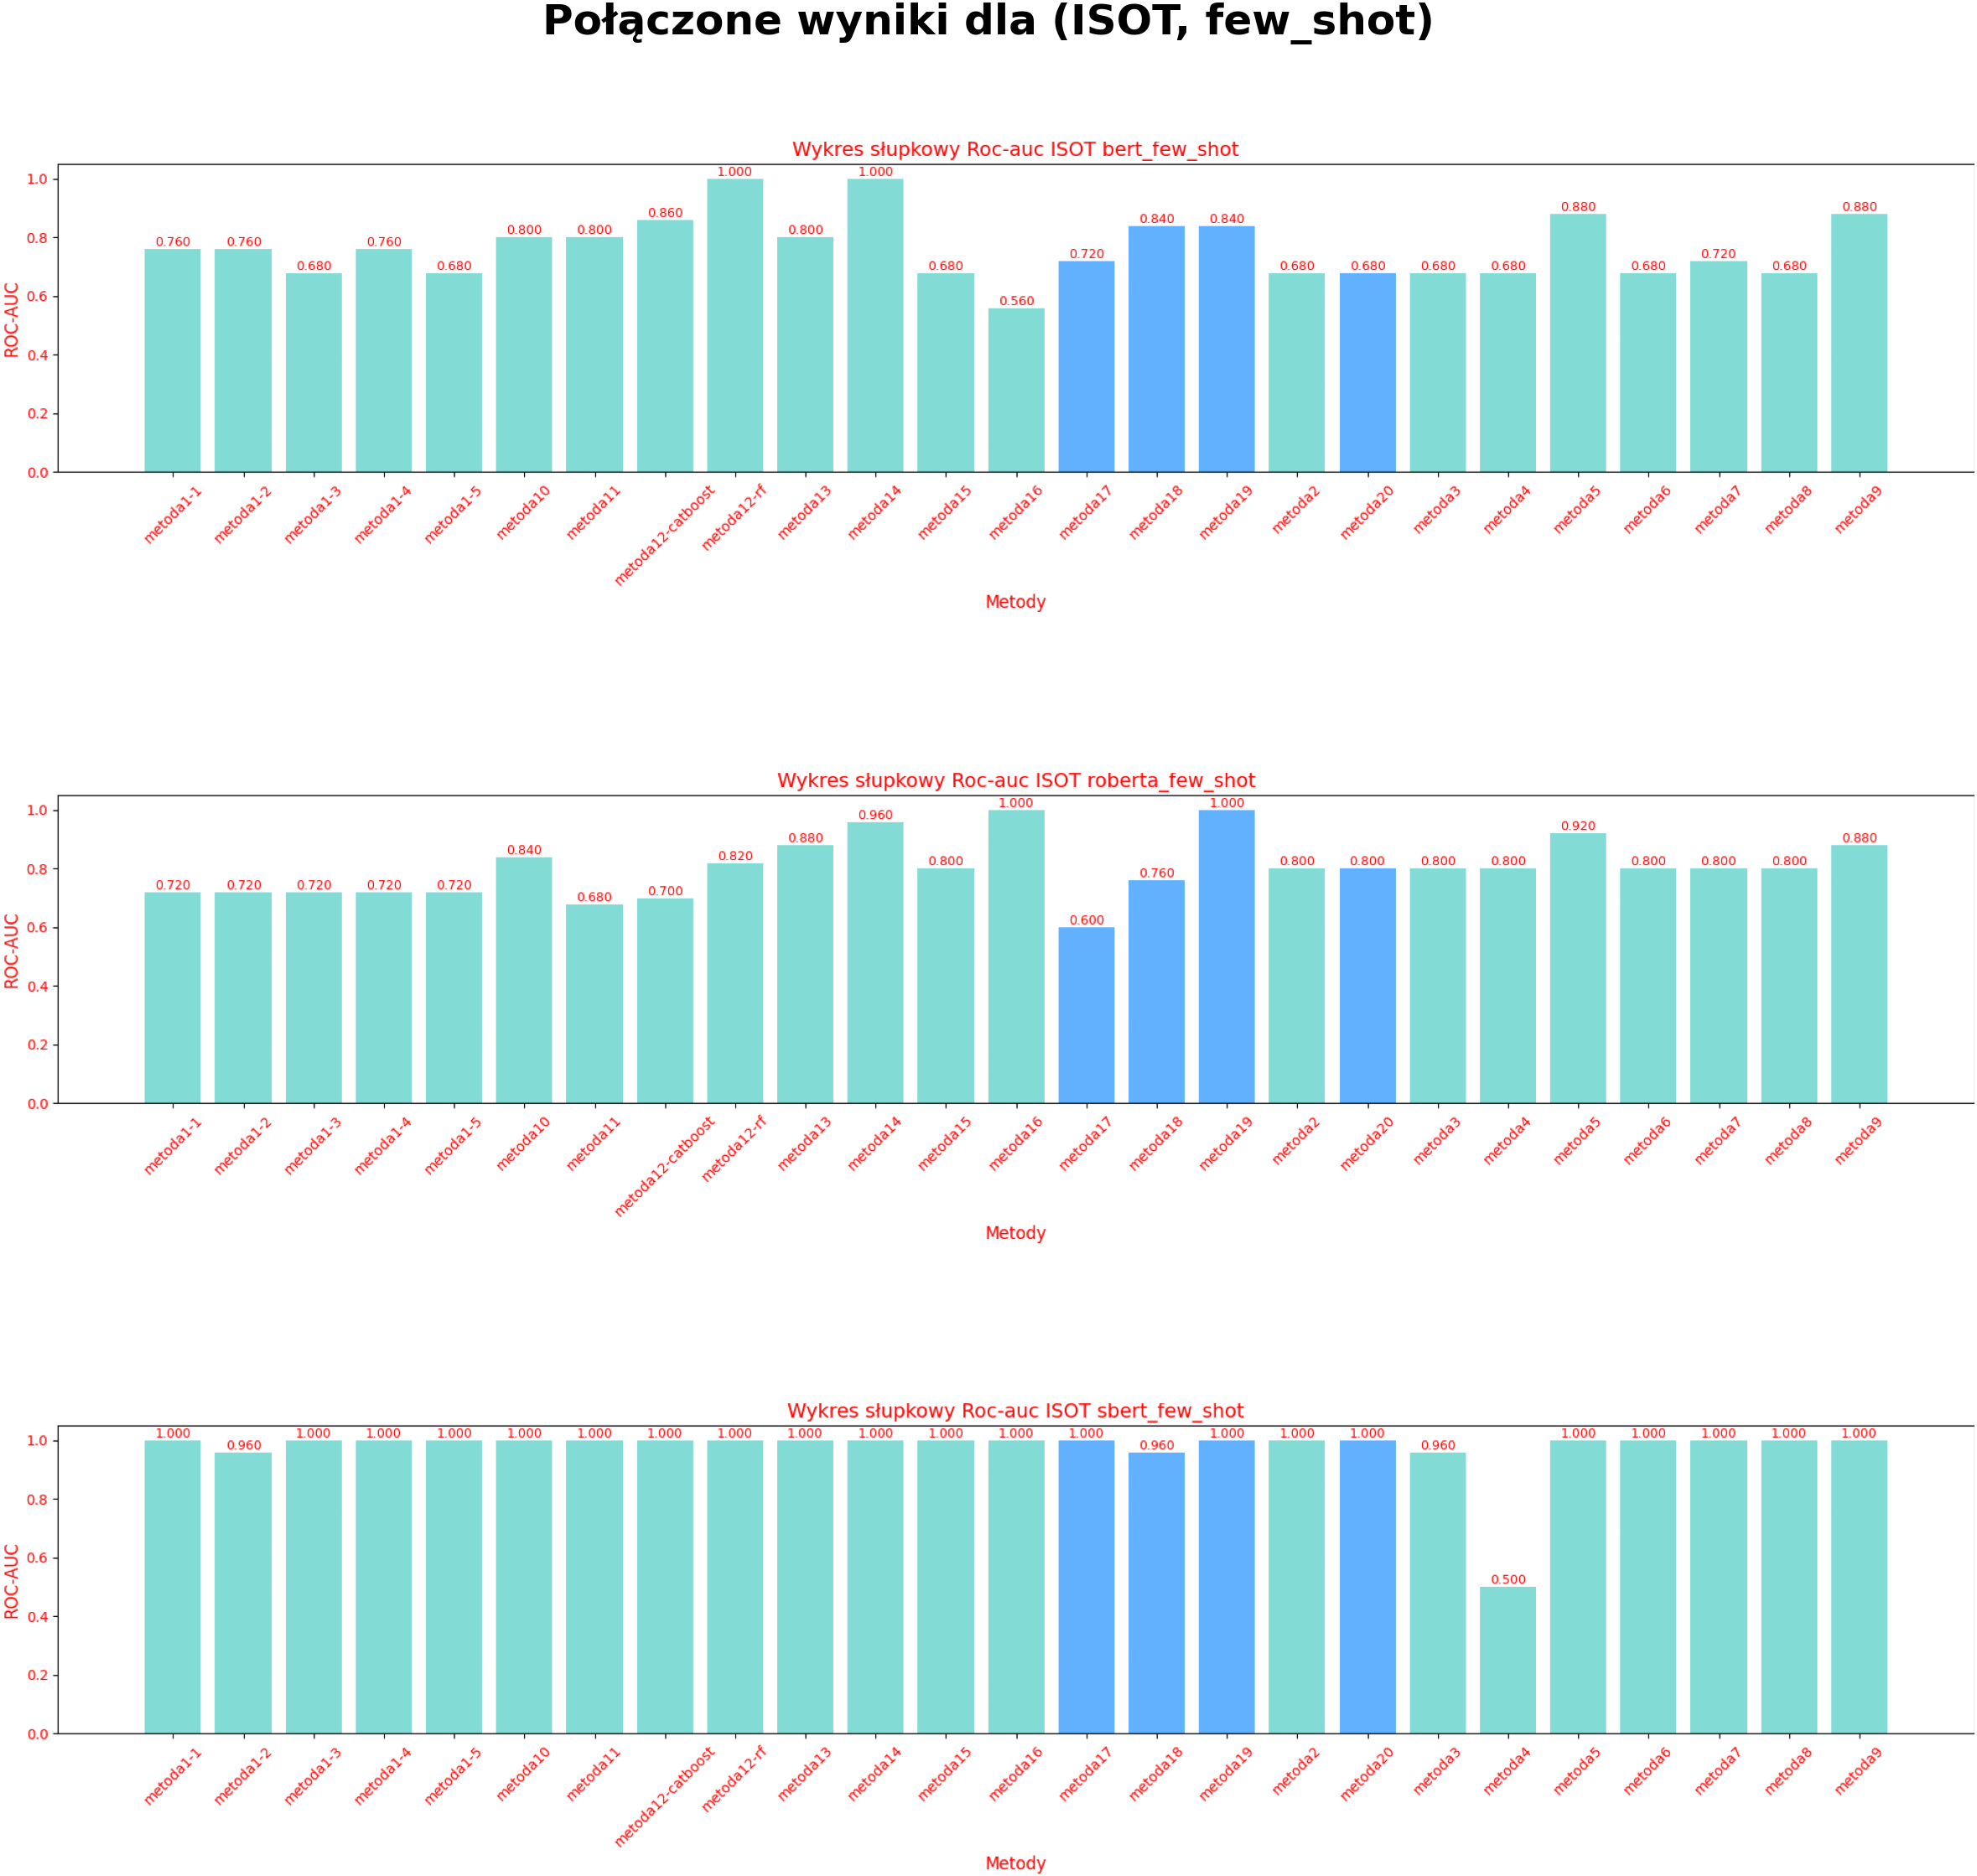
\includegraphics[width=0.99\textwidth]{img/stats/ISOT_few_shot/ISOT_few_shot_Combined_ROC-AUC_bar.png}
	\caption{Histogram rozkładu \textbf{Pola pod krzywą ROC-AUC (ROC-AUC)}.}
	\label{fig:isot_few_shot_roc}
\end{figure}

\subsubsection{Czas wykonania}
Wykres liniowy \textbf{Czasu wykonania (Execution Time)} \ref{fig:isot_few_shot_prcurve} przedstawia porównanie czasu potrzebnego na wykonanie predykcji przez poszczególne metody dla różnych embeddingów językowych. Na podstawie wykresów można sformułować następujące obserwacje:

\begin{itemize}
	\item \textbf{Wykres górny (BERT):}
	      \begin{itemize}
		      \item Najwięcej czasu zajęły metody \texttt{Metoda9} oraz \texttt{Metoda20} – powyżej 500 sekund. \texttt{Metoda9} jest czasochłonna z powodu iteracyjnych algorytmów ensemble oraz kosztownego KNN na embeddingach BERT. \texttt{Metoda20}, wykorzystująca stacking z LightGBM, CatBoost, Random Forest i Gradient Boosting, wymaga znacznego czasu ze względu na trenowanie czterech modeli bazowych na dużych danych BERT.
		      \item Najkrótszy czas wykonania miały \texttt{Metoda18}, \texttt{Metoda7} oraz \texttt{Metoda10} – mniej niż 20 sekund. \texttt{Metoda18} osiąga wysoką efektywność dzięki swojej architekturze po raz kolejny. \texttt{Metoda7} i \texttt{Metoda10} reprezentują szybkie przetwarzanie informatywnych cech BERT.
	      \end{itemize}

	\item \textbf{Wykres środkowy (RoBERTa):}
	      \begin{itemize}
		      \item Najwięcej czasu zajęły metody \texttt{Metoda14}, \texttt{Metoda9} oraz \texttt{Metoda17} – od 200 do 500 sekund. \texttt{Metoda17} wymaga dodatkowego czasu na optymalizację hiperparametrów i trenowanie złożonych modeli bazowych, co jest bardziej kosztowne niż w poprzednich eksperymentach (10–60 sekund). Czas wykonania \texttt{Metoda17} i \texttt{Metoda9} w porównaniu do wcześniejszych eksperymentów sugeruje bardziej złożoną strukturę RoBERTa.
		      \item Najkrótszy czas wykonania miały \texttt{Metoda18}, \texttt{Metoda7} oraz \texttt{Metoda10} – mniej niż 20 sekund, powów takiej efektywności czasowej pozostaje podobny jak w przypadku \texttt{BERT}.
	      \end{itemize}

	\item \textbf{Wykres dolny (SBERT):}
	      \begin{itemize}
		      \item Najdłuższy czas działania osiągnęła \texttt{Metoda4} – około 2000 sekund. \texttt{Metoda4}, łącząca Bi-LSTM, CNN i MLP, jest wyjątkowo czasochłonna z powodu złożonych warstw sekwencyjnych, operacji konwolucyjnych.
		      \item Najkrótszy czas uzyskano dla \texttt{Metoda7} oraz \texttt{Metoda19} – do 50 sekund. \texttt{Metoda7} wykorzystuje prosty algorytm, wybierając losowe podzbiory drze, co pozwala na szybkie przetwarzanie danych. \texttt{Metoda7} utrzymuje swoją efektywność z wcześniejszych eksperymentów, podczas gdy \texttt{Metoda19} jest wolniejsza niż w najszybszych przypadkach, ale wciąż znacznie szybsza od \texttt{Metoda4}.
	      \end{itemize}
\end{itemize}

Analiza wykresów czasu wykonania pokazuje, że efektywność czasowa metod zależy od ich architektury, specyfiki embeddingów oraz charakterystyki danych w danym eksperymencie. Złożone modele, takie jak \texttt{Metoda4}, \texttt{Metoda9}, \texttt{Metoda14}, \texttt{Metoda17} i \texttt{Metoda20}, są czasochłonne z powodu głębokich sieci, iteracyjnych algorytmów ensemble, optymalizacji hiperparametrów lub dużej liczby próbek, szczególnie dla RoBERTa i SBERT. \texttt{Metoda4} i \texttt{Metoda20} wykazują znaczne pogorszenie efektywności w porównaniu do wcześniejszych eksperymentów, co sugeruje wpływ większych lub bardziej złożonych danych. \texttt{Metoda19}, wcześniej wyjątkowo szybka dla SBERT, jest wolniejsza, ale pozostaje efektywna. Prostsze metody, takie jak \texttt{Metoda7}, \texttt{Metoda10} i \texttt{Metoda18}, osiągają krótsze czasy dzięki zoptymalizowanym modelom i efektywnemu wykorzystaniu cech, szczególnie dla SBERT. Zróżnicowanie czasów wykonania podkreśla konieczność dopasowania architektury modelu i optymalizacji hiperparametrów do specyfiki danych i typu embeddingu.
\begin{figure}[H]
	\centering
	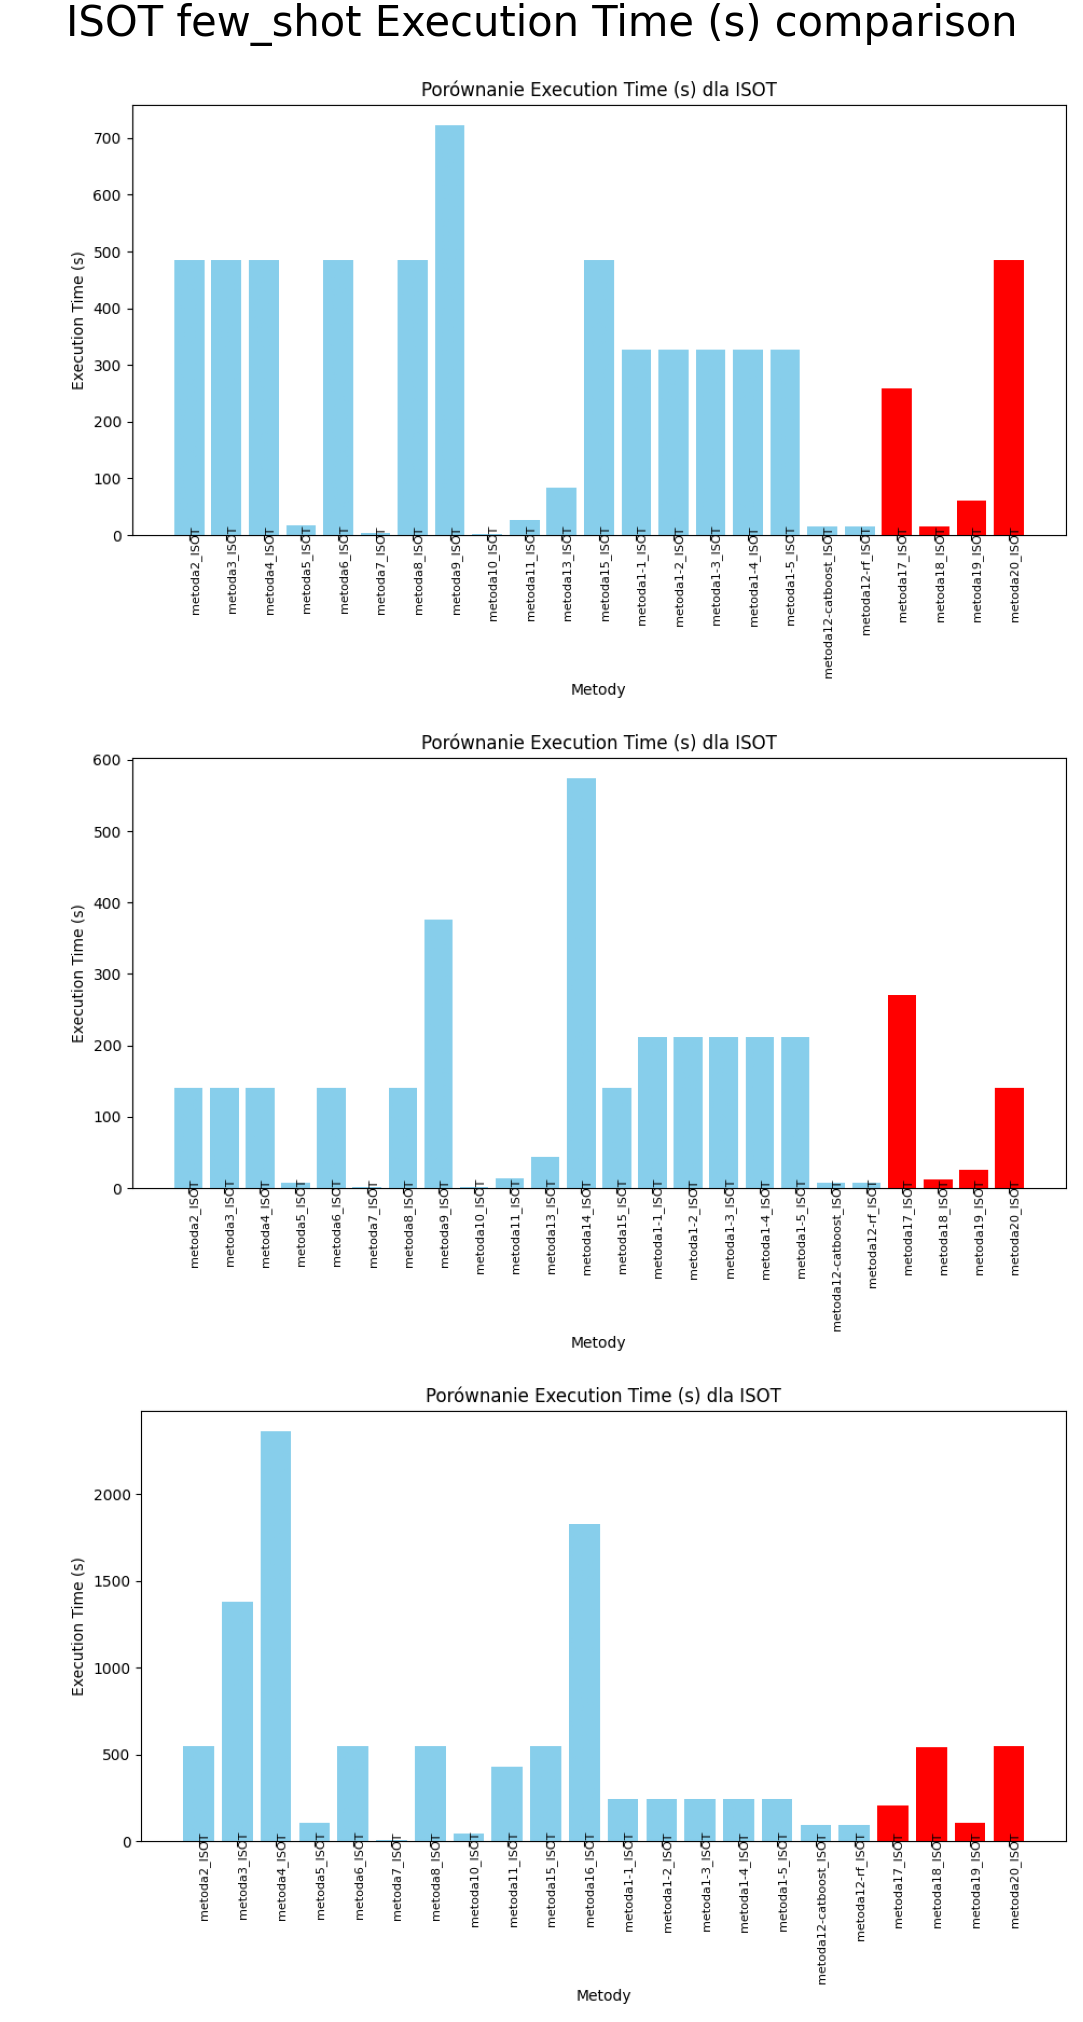
\includegraphics[width=0.99\textwidth]{img/stats/ISOT_few_shot/ISOT_few_shot_Execution Time (s)_comparison.png}
	\caption{\textbf{Czas wykonania (Execution Time)} w sekundach.}
	\label{fig:isot_few_shot_prcurve}
\end{figure}

\subsection{Wyniki w trybie one-shot}
W trybie \textbf{one-shot} dla datasetu \textbf{ISOT}. Poniżej przedstawiono szczegółowy opis wyników w formie histogramów, które ilustrują rozkłady kluczowych metryk, oraz wykresu liniowego czasu wykonania eksperymentów.
\subsubsection{Accuracy}
Wykresy słupkowe \textbf{Dokładności (Accuracy)} \ref{fig:isot_one_shot_accuracy} pokazuje rozkład wartości dokładności dla wszystkich metod. Analizując podany wykres słupkowy można zauważyć następujące rozkłady wyników:
\begin{itemize}
	\item \textbf{Wykres górny (BERT):}
	      \begin{itemize}
		      \item Najlepsze wyniki, w zakresie 0.45 - 0.5 dokładności, osiągnęły metody: \texttt{Metoda12-catboost}, \texttt{Metoda13}, \texttt{Metoda14}, \texttt{Metoda15}, \texttt{Metoda2}, \texttt{Metoda3} oraz autorska \texttt{Metoda20}. Ten zakres wyników, choć umiarkowany, świadczy o zdolności tych metod do radzenia sobie z wyzwaniem one-shot learningu z embeddingami BERT. Ich sukces może wynikać ze zbalansowanych architektur lub skutecznych technik ensemble, które pozwalają na generalizację z bardzo ograniczonej liczby przykładów.
		      \item Najgorsze wyniki odnotowano dla wszystkich pozostałych metod. Taki rozkład sugeruje, że w przypadku embeddingów BERT w scenariuszu one-shot, większość metod ma znaczące trudności w efektywnym uczeniu się i generalizowaniu, co jest spowodowane zbyt niską liczbą danych do treningu.
	      \end{itemize}

	\item \textbf{Wykres środkowy (RoBERTa):}
	      \begin{itemize}
		      \item Najlepsze wyniki, w okolicach $0.95 - 1.0$ dokładności, osiągnęły metody takie jak \texttt{Metoda12-catboost}, \texttt{Metoda11}, \texttt{Metoda1-10}, \texttt{Metoda1-5}, \texttt{Metoda1-3}. Wyniki bliskie 100\% dla tej grupy metod są wyjątkowe i wskazują, że embeddingi RoBERTa są niezwykle informatywne i łatwo separowalne, nawet w scenariuszu one-shot. Te metody są w stanie perfekcyjnie nauczyć się klasyfikacji z pojedynczego przykładu, co świadczy o wysokiej jakości reprezentacji dostarczanych przez RoBERTa oraz o zdolności tych modeli do ich efektywnego wykorzystania.
		      \item Najgorsze wyniki odnotowano dla metody \texttt{Metoda13}. Słaby wynik dla tej metody jest zaskakujący w obliczu dominujących wysokich wyników dla RoBERTa. Może to wskazywać na problem ze specyficzną konfiguracją \texttt{Metoda13} w tym scenariuszu, między tym nieoptymalne wykorzystanie techniki SMOTETomek lub błędy w jej implementacji, które uniemożliwiły jej efektywne wykorzystanie danych RoBERTa.
	      \end{itemize}

	\item \textbf{Wykres dolny (SBERT):}
	      \begin{itemize}
		      \item Najlepsze wyniki osiągnęły praktycznie wszystkie metody. Ten wynik jest wyjątkowy i sugeruje, że embeddingi SBERT są zbyt informatywne i "łatwe" do klasyfikacji nawet w kontekście one-shot learningu, pozwalając większości algorytmów na osiągnięcie wysokiej dokładności. Może to wynikać z ich zdolności do tworzenia bardzo spójnych i znaczących reprezentacji semantycznych, które ułatwiają modelom odróżnianie klas na podstawie bardzo ograniczonych danych.
		      \item Najgorsze wyniki odnotowano dla metody \texttt{Metoda4}. Niska dokładność tej metody jest zaskakująca, zwłaszcza w kontekście ogólnej wysokiej wydajności innych metod dla SBERT. \texttt{Metoda4}, będąca architekturą opartą na zespole sieci Bi-LSTM, CNN i MLP, jest modelem głębokiego uczenia. Jej słabe wyniki mogą wynikać z trudności w efektywnym trenowaniu tak złożonej architektury na bardzo ograniczonej liczbie przykładów dostępnych w scenariuszu one-shot, co prowadzi do niedostatecznej generalizacji i niskiej dokładności.
	      \end{itemize}
\end{itemize}

Analiza wykresów słupkowych dokładności dla one-shot learningu ukazuje znaczące różnice w wydajności metod w zależności od typu zastosowanego embeddingu. Embeddingi RoBERTa i SBERT wydają się być szczególnie dobrze przystosowane do zadań one-shot, umożliwiając osiągnięcie wysokiej, a nawet niemal perfekcyjnej dokładności dla wielu metod. To świadczy o ich zdolności do generowania bardzo spójnych i łatwo separowalnych reprezentacji, nawet przy minimalnej liczbie przykładów.

W przypadku BERT, wyniki są znacznie niższe, co sugeruje, że choć embeddingi są bogate w informacje, to efektywne uczenie się z pojedynczych przykładów w tym kontekście jest znacznie trudniejsze. Wśród metod autorskich, \texttt{Metoda20} wyróżnia się dla osadzeń BERT, natomiast żadna z metod autorskich nie znalazła się wśród najlepszych dla RoBERTa, co jest nietypowe, zważywszy na ich dobrą wydajność w innych kategoriach. Z kolei dla SBERT, autorskie metody są częścią grupy osiągającej najlepsze wyniki (przykładowo \texttt{Metoda17}, \texttt{Metoda18} mogą być w tej grupie "wszystkich metod"), co świadczy o ich zdolności do wykorzystania wysokiej jakości reprezentacji SBERT. Słabe wyniki niektórych metod, takich jak \texttt{Metoda13} dla RoBERTa czy \texttt{Metoda4} dla SBERT, podkreślają konieczność precyzyjnej optymalizacji i dostosowania architektury modelu do specyfiki zarówno embeddingu, jak i wyzwań one-shot learningu.
\begin{figure}[H]
	\centering
	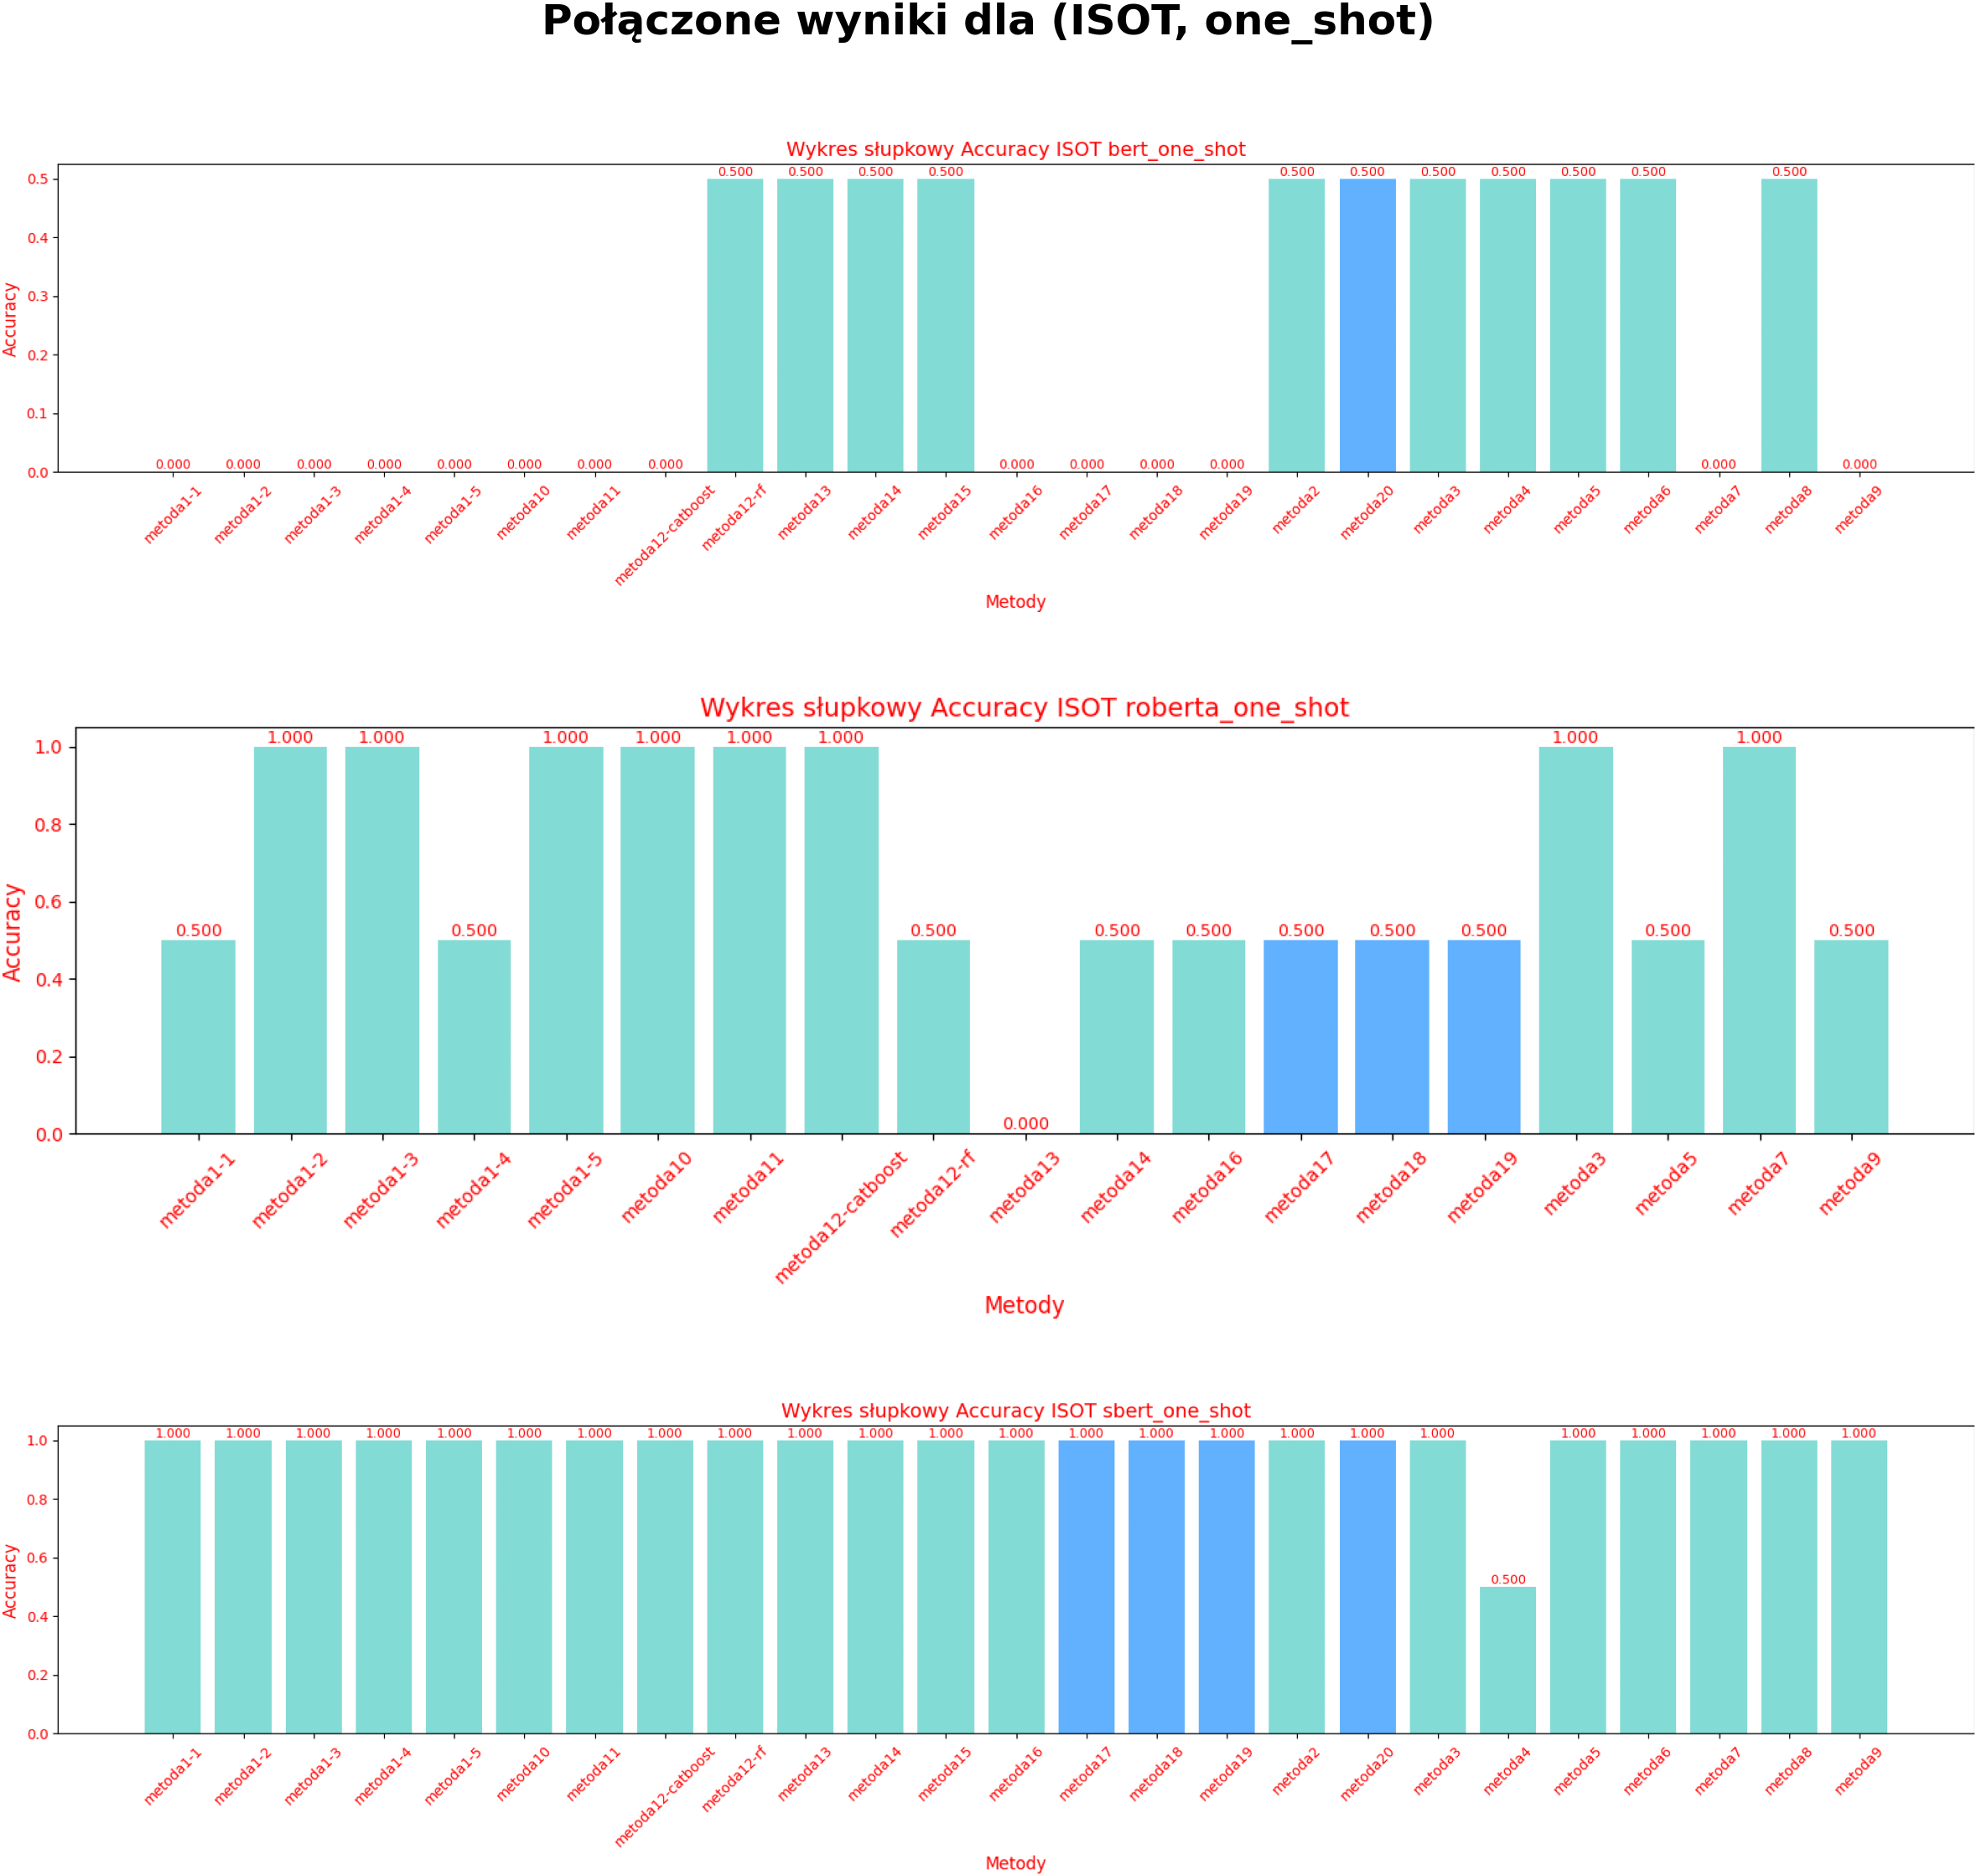
\includegraphics[width=0.99\textwidth]{img/stats/ISOT_one_shot/ISOT_one_shot_Combined_Accuracy_bar_chart.png}
	\caption{Histogram rozkładu \textbf{Dokładności (Accuracy)}.}
	\label{fig:isot_one_shot_accuracy}
\end{figure}

\subsubsection{F1-Score}
Wykresy słupkowe \textbf{Wyniku F1 (F1-Score)} \ref{fig:isot_one_shot_f1} przedstawia rozkład wartości F1-Score dla wszystkich analizowanych metod. Na podstawie wykresu można sformułować następujące obserwacje:

\begin{itemize}
	\item \textbf{Wykres górny (BERT):}
	      \begin{itemize}
		      \item Najwyższe wartości F1-Score osiągnęły metody takie jak \texttt{Metoda12\-rf}, \texttt{Metoda13}, \texttt{Metoda14}, \texttt{Metoda15}, \texttt{Metoda2}, \texttt{Metoda3}, \texttt{Metoda4}, \texttt{Metoda5}, \texttt{Metoda6} oraz wśród autorskich \texttt{Metoda20}. Wysokie wartości F1-Score dla tej grupy metod wskazują na ich zdolność do efektywnego balansu między precyzją a recall, co jest kluczowe w scenariuszu one-shot z embeddingami BERT. Sukces tych metod, w tym szczególnie dla \texttt{Metoda20}, wynika z jej umiejętności efektywnego uchwycenia i uogólnienia wzorców z pojedynczych przykładów, pomimo ogólnie niższego poziomu trudności dla BERT w one-shot learningu.
		      \item Najniższe wyniki posiadają pozostałe metody. Taki rozkład sugeruje, że dla embeddingów BERT w trybie one-shot, większość metod ma znaczące trudności w osiągnięciu zbalansowanej wydajności precyzji i recall. Może to być spowodowane ich niezdolnością do skutecznego wyodrębniania informatywnych cech z bardzo ograniczonej liczby przykładów, co prowadzi do słabych wyników F1-Score.
	      \end{itemize}
	\item \textbf{Wykres środkowy (RoBERTa):}
	      \begin{itemize}
		      \item Najlepsze rezultaty uzyskały metody z grupy: \texttt{Metoda1\-2}, \texttt{Metoda1\-3}, \texttt{Metoda1\-5}, \texttt{Metoda10}, \texttt{Metoda12\-catboost}. Wyniki bliskie perfekcji dla tej grupy metod są wyjątkowe i wskazują, że embeddingi RoBERTa są niezwykle informatywne i łatwo separowalne, nawet w scenariuszu one-shot. Te metody są w stanie perfekcyjnie nauczyć się klasyfikacji z pojedynczego przykładu, co świadczy o wysokiej jakości reprezentacji dostarczanych przez RoBERTa oraz o zdolności tych modeli do ich efektywnego wykorzystania.
		      \item Najsłabsze wyniki posiada większość innych metod, wśród nich autorskie \texttt{Metoda17} i \texttt{Metoda19}. Niska wartość F1-Score dla tych metod, w tym dla zaawansowanych modeli ensemble jak \texttt{Metoda17} (zaawansowany VotingClassifier) i \texttt{Metoda19} (model stackingowy), jest zaskakująca w obliczu dominujących wysokich wyników dla RoBERTa. Może to wskazywać na nieoptymalny dobór klasyfikatorów bazowych w tym przypadku lub trudności w adaptacji tych konkretnych architektur do specyfiki one-shot learningu z embeddingami RoBERTa, co skutkowało niezbalansowaną precyzją i recall.
	      \end{itemize}
	\item \textbf{Wykres dolny (SBERT):}
	      \begin{itemize}
		      \item Najlepsze wartości wyników należą praktycznie do wszystkich metod. Ten wynik jest wyjątkowy i sugeruje, że embeddingi SBERT są wysoce informatywne i "łatwe" do klasyfikacji, nawet w kontekście one-shot learningu, pozwalając większości algorytmów na osiągnięcie niemal perfekcyjnej wartości F1-Score. Może to wynikać z ich zdolności do tworzenia bardzo spójnych i znaczących reprezentacji semantycznych, które ułatwiają modelom zbalansowane odróżnianie klas na podstawie bardzo ograniczonych danych.
		      \item Najgorsze rezultaty zaobserwowano dla \texttt{Metoda4}, na poziomie 0.70. Niska wartość F1-Score dla tej metody, pomimo ogólnie doskonałych wyników dla SBERT, sugeruje, że w tym konkretnym przypadku mogła ona mieć trudności z optymalizacją. \texttt{Metoda4}, będąca architekturą opartą na zespole sieci Bi-LSTM, CNN i MLP, jest modelem głębokiego uczenia. Jej słabe wyniki mogą wynikać z trudności w efektywnym trenowaniu tak złożonej architektury na bardzo ograniczonej liczbie przykładów dostępnych w scenariuszu one-shot, co skutkowało niezbalansowaną wydajnością precyzji i recall.
	      \end{itemize}
\end{itemize}

Analiza wykresów słupkowych F1-Score dla one-shot learningu ujawnia znaczące różnice w wydajności metod w zależności od typu zastosowanego embeddingu. Embeddingi RoBERTa i SBERT wydają się być szczególnie dobrze przystosowane do zadań one-shot, umożliwiając osiągnięcie wysokiej, a nawet niemal perfekcyjnej wartości F1-Score dla wielu metod. To świadczy o ich zdolności do generowania bardzo spójnych i łatwo separowalnych reprezentacji, nawet przy minimalnej liczbie przykładów.

W przypadku BERT, wyniki są znacznie niższe, co sugeruje, że choć embeddingi są bogate w informacje, to efektywne uczenie się z pojedynczych przykładów w tym kontekście jest znacznie trudniejsze. Wśród metod autorskich, \texttt{Metoda20} wyróżnia się dla osadzeń BERT. Z kolei dla RoBERTa, zaskakująco słabe wyniki odnotowały autorskie \texttt{Metoda17} i \texttt{Metoda19}, co wskazuje na potrzebę dalszej optymalizacji tych konkretnych architektur ensemble dla tego typu embeddingu i scenariusza. Dla SBERT, autorskie metody są częścią grupy osiągającej najlepsze wyniki (\texttt{Metoda17}, \texttt{Metoda20}), co świadczy o ich zdolności do wykorzystania wysokiej jakości reprezentacji SBERT.
\begin{figure}[H]
	\centering
	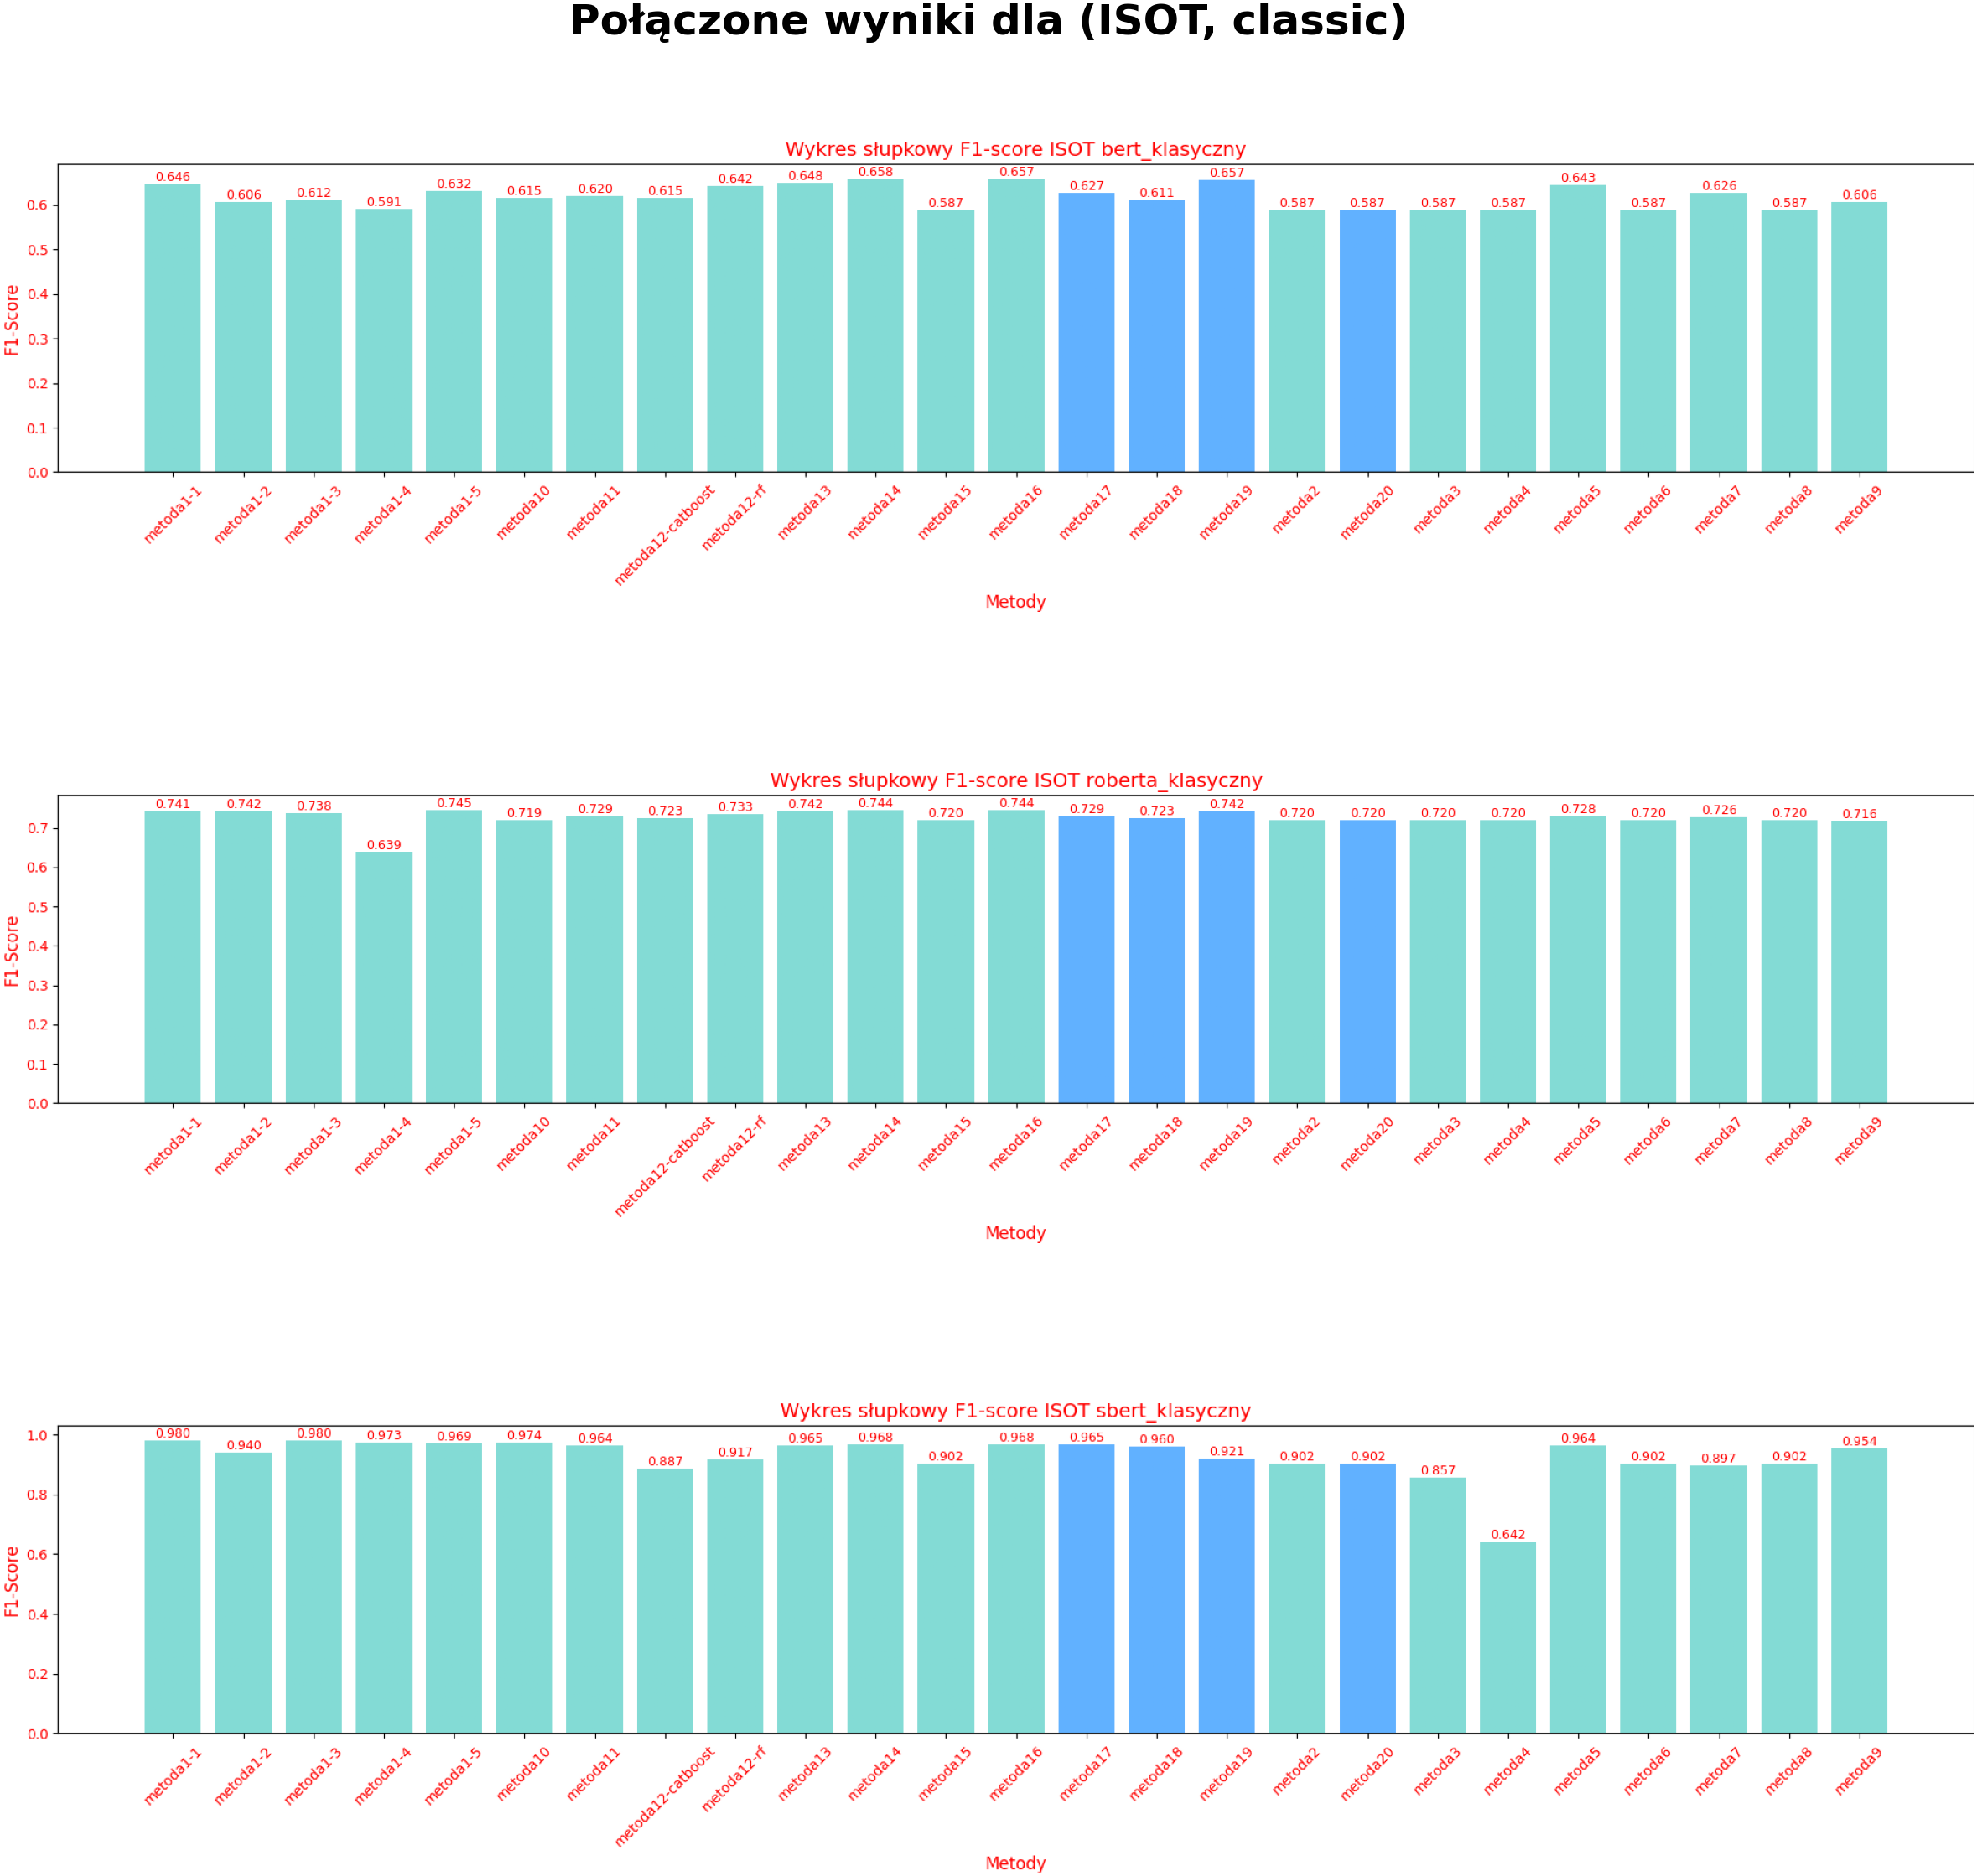
\includegraphics[width=0.99\textwidth]{img/stats/ISOT_classic/ISOT_classic_Combined_F1-Score_bar.png}
	\caption{Histogram rozkładu \textbf{Wyniku F1 (F1-Score)}.}
	\label{fig:isot_one_shot_f1}
\end{figure}

\subsubsection{ROC-AUC}
Wykresy słupkowe \textbf{Pola pod krzywą ROC-AUC (ROC-AUC)} \ref{fig:isot_one_shot_roc} przedstawia rozkład wartości ROC-AUC dla wszystkich badanych metod. Na podstawie wykresu można sformułować następujące obserwacje:

\begin{itemize}
	\item \textbf{Wykres górny (BERT):}
	      \begin{itemize}
		      \item Bardzo słabe wyniki odnotowano dla wszystkich metod. Ten wynik jest krytyczny i sugeruje, że embeddingi BERT w scenariuszu one-shot learningu, w przeciwieństwie do innych embeddingów, nie są w stanie dostarczyć wystarczająco informatywnych i separowalnych cech, aby modele mogły skutecznie rozróżniać klasy. Może to wynikać z ogólnych trudności w generalizowaniu na tak małej liczbie przykładów przy wykorzystaniu specyficznych właściwości embeddingów BERT.
	      \end{itemize}

	\item \textbf{Wykres środkowy (RoBERTa):}
	      \begin{itemize}
		      \item Najlepsze wartości ROC-AUC osiągnęły autorskie metody \texttt{Metoda17} (zaawansowany VotingClassifier) oraz \texttt{Metoda18} (model stackingowy z GradientBoosting i CatBoost), wraz z \texttt{Metoda11}, \texttt{Metoda10} i innymi. Wysoka wartość ROC-AUC dla tych metod wskazuje na ich efektywność w przetwarzaniu embeddingów RoBERTa i osiąganiu doskonałej zdolności rozróżniania klas. To świadczy o zdolności tych modeli, zwłaszcza zaawansowanych ensemble, do wydobywania istotnych wzorców z danych, nawet w trybie one-shot.
		      \item Najgorsze rezultaty zaobserwowano dla autorskich \texttt{Metoda16} (model stackingowy z meta-klasyfikatorem), \texttt{Metoda19} (model stackingowy) i dodatkowo \texttt{Metoda5}, \texttt{Metoda12-rf}. Niska wartość ROC-AUC dla tych metod, w tym dla złożonych autorskich modeli ensemble, jest zaskakująca. Może to wskazywać na nieoptymalny dobór modeli bazowych, niewłaściwe ważenie w VotingClassifierze, lub trudności w adaptacji tych konkretnych architektur do specyfiki one-shot learningu z embeddingami RoBERTa, co skutkuje słabą zdolnością do rozróżniania klas.
	      \end{itemize}

	\item \textbf{Wykres dolny (SBERT):}
	      \begin{itemize}
		      \item Najlepsze wartości ROC-AUC osiągnęły wszystkie metody oprócz jednej. Ten wynik jest wyjątkowy i sugeruje, że embeddingi SBERT są wysoce informatywne i "łatwe" do klasyfikacji, nawet w kontekście one-shot learningu, pozwalając większości algorytmów na osiągnięcie niemal perfekcyjnej zdolności rozróżniania klas. Może to wynikać z ich zdolności do tworzenia bardzo spójnych i znaczących reprezentacji semantycznych, które ułatwiają modelom odróżnianie klas na podstawie bardzo ograniczonych danych.
		      \item Słabe rezultaty zaobserwowano dla \texttt{Metoda4} (architektura oparta na zespole sieci Bi-LSTM, CNN i MLP). Niska wartość ROC-AUC dla tej metody, pomimo ogólnie doskonałych wyników dla SBERT, sugeruje, że w tym konkretnym przypadku mogła ona mieć trudności z optymalizacją. Jej złożona architektura, mimo potencjału, mogła nie być w stanie efektywnie nauczyć się z bardzo ograniczonej liczby przykładów w scenariuszu one-shot, co prowadzi do słabej zdolności rozróżniania klas, nawet przy wysokiej jakości danych wejściowych z SBERT.
	      \end{itemize}
\end{itemize}

Analiza wykresów słupkowych ROC-AUC dla one-shot learningu ukazuje znaczące różnice w wydajności metod w zależności od typu zastosowanego embeddingu. Embeddingi RoBERTa i SBERT wydają się być szczególnie dobrze przystosowane do zadań one-shot, umożliwiając osiągnięcie wysokiej, a nawet niemal perfekcyjnej zdolności rozróżniania klas dla wielu metod. To świadczy o ich zdolności do generowania bardzo spójnych i łatwo separowalnych reprezentacji, nawet przy minimalnej liczbie przykładów.

W przeciwieństwie do RoBERTa i SBERT, dla BERT odnotowano bardzo słabe wyniki dla wszystkich metod, co podkreśla, że one-shot learning z tymi embeddingami jest znacznie trudniejszy. Wśród metod autorskich, \texttt{Metoda17} i \texttt{Metoda18} wyróżniają się dla osadzeń RoBERTa, osiągając wysokie ROC-AUC. Z kolei dla SBERT, autorskie metody są częścią grupy osiągającej najlepsze wyniki (włączając w to \texttt{Metoda17}, \texttt{Metoda18}, \texttt{Metoda19}, \texttt{Metoda20} wśród "wszystkich metod"), co świadczy o ich zdolności do wykorzystania wysokiej jakości reprezentacji SBERT. Słabe wyniki niektórych autorskich metod, takich jak \texttt{Metoda19} dla RoBERTa, podkreślają konieczność precyzyjnej optymalizacji i dostosowania architektury modelu do specyfiki zarówno embeddingu, jak i wyzwań one-shot learningu.
\begin{figure}[H]
	\centering
	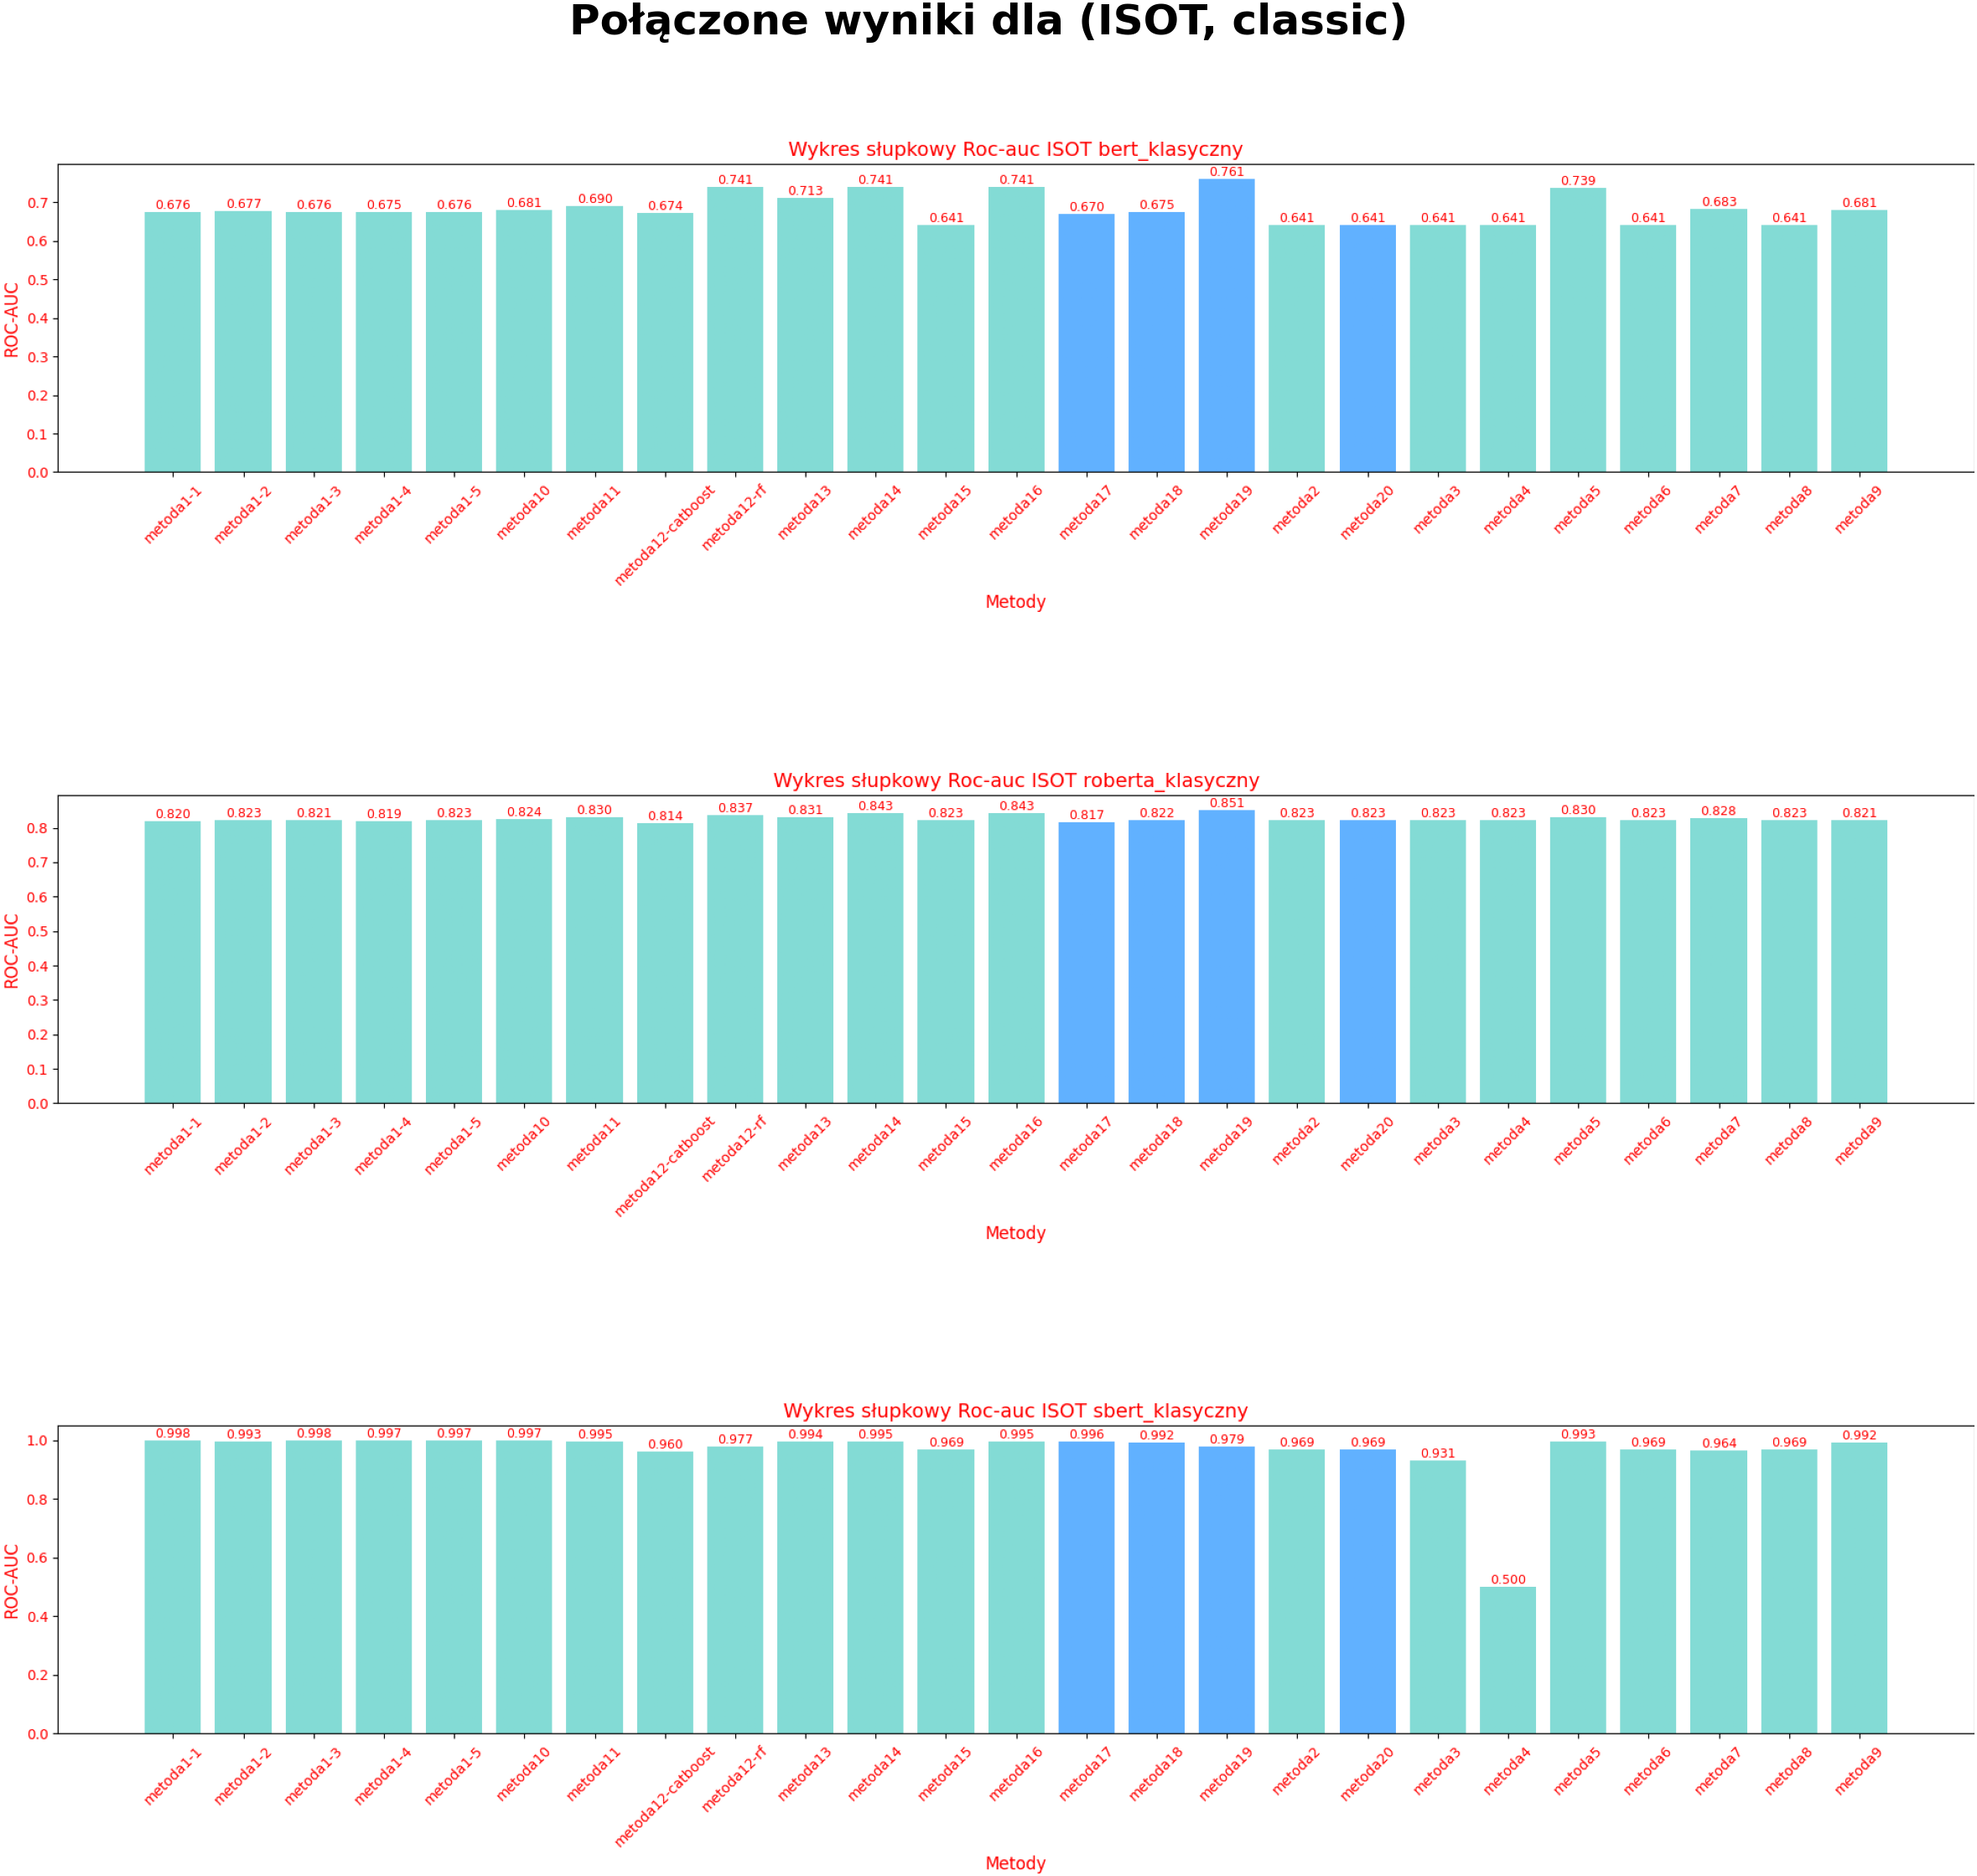
\includegraphics[width=0.99\textwidth]{img/stats/ISOT_classic/ISOT_classic_Combined_ROC-AUC_bar.png}
	\caption{Histogram rozkładu \textbf{Pola pod krzywą ROC-AUC (ROC-AUC)}.}
	\label{fig:isot_one_shot_roc}
\end{figure}

\subsubsection{Czas wykonania}
Wykres liniowy \textbf{Czasu wykonania (Execution Time)} \ref{fig:isot_one_shot_prcurve} przedstawia porównanie czasu potrzebnego na wykonanie predykcji przez poszczególne metody dla różnych embeddingów językowych. Na podstawie wykresów można sformułować następujące obserwacje dotyczące efektywności czasowej oraz przyczyn zróżnicowania wyników, z uwzględnieniem zmienności wydajności metod w porównaniu do wcześniejszych eksperymentów:

\begin{itemize}
	\item \textbf{Wykres górny (BERT):}
	      \begin{itemize}
		      \item Najdłuższy czas wykonania, wynoszący około 140 sekund, odnotowano dla metod \texttt{Metoda2}, \texttt{Metoda3}, \texttt{Metoda4}, \texttt{Metoda8}, \texttt{Metoda15} oraz \texttt{Metoda20}. \texttt{Metoda2}, wykorzystująca Gradient Boosting i MLP na podzbiorach cech z meta-modelem regresji logistycznej, jest czasochłonna. \texttt{Metoda4} podobnie jak poprzednio wspominaliśmy, wymaga intensywnych obliczeń z powodu sekwencyjnych warstw. \texttt{Metoda20} wykazuje pogorszenie w porównaniu do wcześniejszych wyników (poniżej 1 sekundy dla BERT), co może wynikać z większej liczby próbek lub bardziej złożonej struktury danych.
		      \item Najkrótszy czas wykonania, poniżej 10 sekund, miały \texttt{Metoda7}, \texttt{Metoda10} oraz \texttt{Metoda18}. \texttt{Metoda18} nadal utrzymuje wysoką efektywność, jak to zuważyliśmy na poprzednich wykresach liniowych porównania czasów wykonania.
	      \end{itemize}

	\item \textbf{Wykres środkowy (RoBERTa):}
	      \begin{itemize}
		      \item Najwięcej czasu zajęła \texttt{Metoda9} - około 400 sekund. \texttt{Metoda9}, oparta na ensemble z Random Forest, Bagging, AdaBoost i VotingClassifier jest czasochłonna z powodu iteracyjnych algorytmów ensemble oraz kosztownego KNN. Czas ten jest spójny z wcześniejszymi eksperymentami (200\-500 sekund), choć nieco krótszy, co może wskazywać na mniejszą liczbę próbek lub lepszą optymalizację w tym eksperymencie.
		      \item Najkrótszy czas wykonania, poniżej 5 sekund, miały \texttt{Metoda7}, \texttt{Metoda18} oraz \texttt{Metoda19}. \texttt{Metoda19}, oparta na stacking z Random Forest, XGBoost i Gradient Boosting z meta-modelem regresji logistycznej, poprawiła swoją efektywność w porównaniu do wcześniejszych eksperymentów (10–14 sekund dla RoBERTa), dzięki zoptymalizowanym hiperparametrom.
	      \end{itemize}

	\item \textbf{Wykres dolny (SBERT):}
	      \begin{itemize}
		      \item Najdłuższy czas działania, przekraczający 1200 sekund, osiągnęła \texttt{Metoda3}. Drastyczny wzrost czasu w porównaniu do wcześniejszych eksperymentów sugeruje większą liczbę próbek lub bardziej złożoną strukturę danych SBERT w tym eksperymencie.
		      \item Najkrótszy czas uzyskano dla \texttt{Metoda7} oraz średni czas wykonania dla \texttt{Metoda17} i \texttt{Metoda19} - w okolicach 100 sekund. \texttt{Metoda19} osiąga relatywnie krótki czas dzięki zoptymalizowanym hiperparametrom i skalowaniu danych, choć jest wolniejsza niż w najlepszych przypadkach (0.2 sekundy dla SBERT). \texttt{Metoda17} poprawiła swoją efektywność w porównaniu do wcześniejszych eksperymentów (200\-500 sekund dla RoBERTa), co może wynikać z lepszej optymalizacji hiperparametrów lub mniejszej liczby próbek w danych SBERT.
	      \end{itemize}
\end{itemize}
Analiza wykresów czasu wykonania pokazuje, że efektywność czasowa metod zależy od ich architektury, specyfiki embeddingów oraz charakterystyki danych w danym eksperymencie. Złożone modele, takie jak \texttt{Metoda2}, \texttt{Metoda3}, \texttt{Metoda4}, \texttt{Metoda8}, \texttt{Metoda9}, \texttt{Metoda15} i \texttt{Metoda20}, są czasochłonne z powodu głębokich sieci, iteracyjnych algorytmów ensemble lub dużej liczby próbek. \texttt{Metoda2}, \texttt{Metoda3} i \texttt{Metoda20} wykazują znaczne pogorszenie efektywności w porównaniu do wcześniejszych eksperymentów, co sugeruje wpływ bardziej złożonych danych. \texttt{Metoda19} i \texttt{Metoda17} poprawiły swoją wydajność dla RoBERTa i SBERT, podczas gdy \texttt{Metoda7} i \texttt{Metoda18} konsekwentnie osiągają krótkie czasy dzięki prostszym modelom i efektywnemu wykorzystaniu cech, szczególnie dla SBERT. Zróżnicowanie czasów wykonania podkreśla konieczność dopasowania architektury modelu i optymalizacji hiperparametrów do specyfiki danych i typu embeddingu.
\begin{figure}[H]
	\centering
	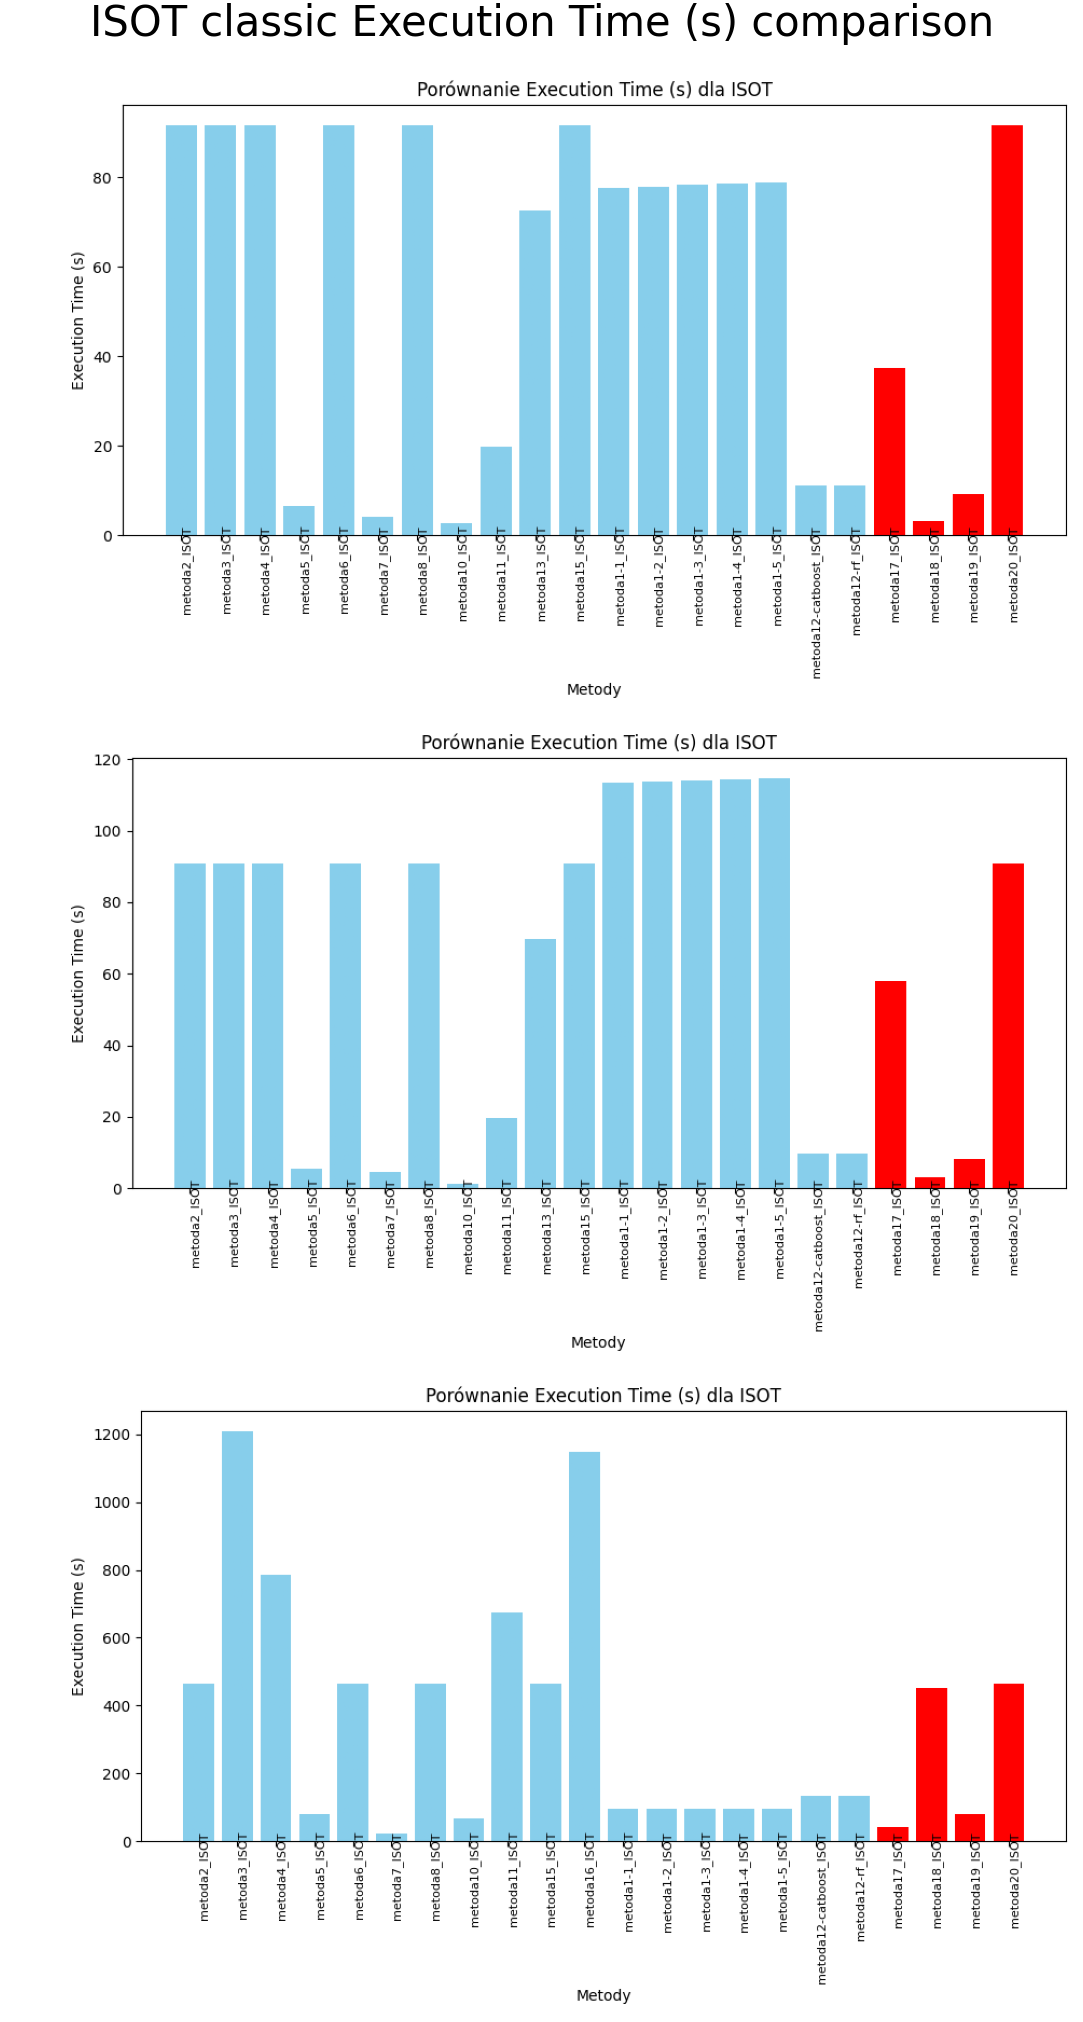
\includegraphics[width=0.99\textwidth]{img/stats/ISOT_classic/ISOT_classic_Execution Time (s)_comparison.png}
	\caption{\textbf{Czas wykonania (Execution Time)} w sekundach.}
	\label{fig:isot_one_shot_prcurve}
\end{figure}

\subsection{Dodatkowa analiza wyników dla datasetu ISOT}
\label{subsec:isot_additional_analysis}
W tej podsekcji przedstawiono szczegółową analizę wyników uzyskanych dla datasetu \textbf{ISOT}, obejmującą wyniki AUC-PR, testy normalności rozkładów, macierze korelacji Pearsona i Spearmana oraz testy statystyczne Kruskal-Wallis. Analiza ma na celu ocenę wydajności wszystkich metod oraz uzasadnienie sensu stosowania bardziej złożonych metod autorskich (\texttt{metoda17}, \texttt{metoda18}, \texttt{metoda19}, \texttt{metoda20}) w kontekście ich potencjalnych zalet w różnych scenariuszach uczenia i specyfiki danych.

\subsubsection{Wyniki AUC-PR}

Poniższa tabela przedstawia wyniki AUC-PR dla różnych metod zastosowanych na datasecie \textbf{ISOT}. Wartości wahają się od 0,6686 do 0,8337, przy czym \texttt{metoda9} osiągnęła najwyższy wynik (0,8337). Wśród metod autorskich (\texttt{metoda17}, \texttt{metoda18}, \texttt{metoda19}, \texttt{metoda20}) najlepszy rezultat odnotowano dla \texttt{metoda18} z wartością 0,8184, co plasuje ją wśród najlepszych metod w tym zestawieniu. Pozostałe metody autorskie (\texttt{metoda17}, \texttt{metoda19}, \texttt{metoda20}) osiągnęły wyniki odpowiednio 0,7865, 0,7633 i 0,7600, co wskazuje na ich zróżnicowaną skuteczność w zależności od kontekstu.

\begin{table}[H]
	\centering
	\caption{Wyniki AUC-PR dla metod na datasecie ISOT}
	\label{tab:isot_auc_pr}
	\begin{tabular}{l r}
		\toprule
		Metoda            & AUC-PR \\
		\midrule
		\texttt{metoda9}           & 0.8337 \\
		\texttt{metoda18}          & 0.8184 \\
		\texttt{metoda10}          & 0.8081 \\
		\texttt{metoda11}          & 0.8061 \\
		\texttt{metoda12-catboost} & 0.7987 \\
		\texttt{metoda7}           & 0.7983 \\
		\texttt{metoda17}          & 0.7865 \\
		\texttt{metoda1-2}         & 0.7841 \\
		\texttt{metoda3}           & 0.7777 \\
		\texttt{metoda1-1}         & 0.7749 \\
		\texttt{metoda14}          & 0.7748 \\
		\texttt{metoda1-4}         & 0.7745 \\
		\texttt{metoda1-3}         & 0.7700 \\
		\texttt{metoda1-5}         & 0.7698 \\
		\texttt{metoda19}          & 0.7633 \\
		\texttt{metoda15}          & 0.7600 \\
		\texttt{metoda2}           & 0.7600 \\
		\texttt{metoda20}          & 0.7600 \\
		\texttt{metoda6}           & 0.7600 \\
		\texttt{metoda8}           & 0.7600 \\
		\texttt{metoda5}           & 0.7521 \\
		\texttt{metoda12-rf}       & 0.7474 \\
		\texttt{metoda13}          & 0.7453 \\
		\texttt{metoda16}          & 0.7206 \\
		\texttt{metoda4}           & 0.6686 \\
		\bottomrule
	\end{tabular}
\end{table}

\subsubsection{Testy normalności i analizy statystyczne}

W testach statystycznych, takich jak Kruskal-Wallis i Shapiro-Wilk, analizowano indywidualne wartości metryk (Accuracy, Precision, Recall, F1-Score, ROC-AUC, MCC, Cohen’s Kappa, AUC-PR) dla każdej metody w ramach datasetu ISOT, w trybach klasycznym, few-shot i one-shot, bez uśredniania wyników między metodami. Próbki stanowią wyniki uzyskane dla każdej metody w danym eksperymencie, co pozwala na bezpośrednie porównanie ich wydajności w kontekście tego samego datasetu i embeddingu (BERT, RoBERTa, SBERT). Na przykład, dla metryki Accuracy w trybie klasycznym, test Kruskal-Wallisa porównuje rozkłady wartości Accuracy dla wszystkich metod (np. \texttt{metoda1-1}, \texttt{metoda18}) w obrębie jednego typu embeddingu.

Testy Shapiro-Wilka wykazały, że większość metryk (Accuracy, Precision, Recall, F1-Score, MCC, Cohen’s Kappa) nie ma rozkładu normalnego (p-value < 0,05) dla wielu metod, co sugeruje asymetrię lub odchylenia od normalności. Wyjątkiem jest metryka ROC-AUC, gdzie tylko \texttt{metoda4} wykazała p-value $\geq$ 0,05 (0,0895), wskazując na możliwość rozkładu normalnego. Dla Accuracy, metody takie jak \texttt{metoda1-1}, \texttt{metoda1-2}, \texttt{metoda1-4}, \texttt{metoda12-rf}, \texttt{metoda14}, \texttt{metoda15}, \texttt{metoda16}, \texttt{metoda17}, \texttt{metoda18}, \texttt{metoda20}, \texttt{metoda2}, \texttt{metoda3}, \texttt{metoda4}, \texttt{metoda5}, \texttt{metoda6}, \texttt{metoda8} osiągnęły p-value $\geq$ 0,05, co może sugerować rozkład zbliżony do normalnego.

Testy Kruskal-Wallisa nie wykazały istotnych statystycznie różnic między metodami dla żadnej metryki w trybach klasycznym, few-shot i one-shot (p-value $\geq$ 0,05), przy czym najwyższe p-value uzyskano dla AUC-PR (0,99998) w trybie klasycznym. Wynik ten wskazuje, że nie ma statystycznie istotnych różnic w wydajności między metodami, w tym między prostszymi (np. \texttt{metoda1-x}) a bardziej złożonymi metodami autorskimi (\texttt{metoda17}, \texttt{metoda18}, \texttt{metoda19}, \texttt{metoda20}). Brak różnic sugeruje, że w niektórych scenariuszach prostsze metody mogą być równie skuteczne, jednak analiza wyników w trybach few-shot i one-shot pokazuje przewagę bardziej złożonych metod w trudniejszych scenariuszach, co omówiono poniżej.

\subsubsection{Analiza korelacji}

Macierze korelacji Pearsona i Spearmana ujawniły silne zależności między metrykami, co ułatwia zrozumienie powiązań między miarami wydajności. Najsilniejsze korelacje dodatnie w macierzy Pearsona zaobserwowano między Accuracy a Cohen’s Kappa (0,9999), Accuracy a MCC (0,9997) oraz MCC a Cohen’s Kappa (0,9997). W macierzy Spearmana korelacje te są równie silne: Accuracy a Cohen’s Kappa (1,0000) oraz Accuracy a MCC (0,9992). Silne korelacje dodatnie występują także między Precision a F1-Score (0,9204 w Pearsonie, 0,8760 w Spearmanie), Recall a F1-Score (0,8864 w Pearsonie, 0,8155 w Spearmanie) oraz ROC-AUC a AUC-PR (0,9305 w Pearsonie, 0,9186 w Spearmanie). Brak silnych ujemnych korelacji wskazuje, że nie ma wyraźnych kompromisów między metrykami, a wysokie korelacje między Accuracy, MCC i Cohen’s Kappa sugerują ich wzajemną zgodność w ocenie wydajności modeli.

\begin{table}[H]
	\centering
	\caption{Kluczowe współczynniki korelacji Pearsona}
	\label{tab:isot_pearson_correlations}
	\begin{tabular}{l r l}
		\toprule
		Para metryk               & Współczynnik Pearsona & Interpretacja         \\
		\midrule
		Accuracy -- Cohen’s Kappa & 0.9999                & Bardzo silna dodatnia \\
		Accuracy -- MCC           & 0.9997                & Bardzo silna dodatnia \\
		MCC -- Cohen’s Kappa      & 0.9997                & Bardzo silna dodatnia \\
		Precision -- F1-Score     & 0.9204                & Silna dodatnia        \\
		Recall -- F1-Score        & 0.8864                & Silna dodatnia        \\
		ROC-AUC -- AUC-PR         & 0.9305                & Bardzo silna dodatnia \\
		\bottomrule
	\end{tabular}
\end{table}

\begin{table}[H]
	\centering
	\caption{Kluczowe współczynniki korelacji Spearmana}
	\label{tab:isot_spearman_correlations}
	\begin{tabular}{l r l}
		\toprule
		Para metryk               & Współczynnik Spearmana & Interpretacja         \\
		\midrule
		Accuracy -- Cohen’s Kappa & 1.0000                 & Bardzo silna dodatnia \\
		Accuracy -- MCC           & 0.9992                 & Bardzo silna dodatnia \\
		MCC -- Cohen’s Kappa      & 0.9992                 & Bardzo silna dodatnia \\
		Precision -- F1-Score     & 0.8760                 & Silna dodatnia        \\
		Recall -- F1-Score        & 0.8155                 & Silna dodatnia        \\
		ROC-AUC -- AUC-PR         & 0.9186                 & Bardzo silna dodatnia \\
		\bottomrule
	\end{tabular}
\end{table}

\subsubsection{Wnioski}
Analizowano indywidualne wartości metryk dla każdej metody w ramach datasetu ISOT, bez uśredniania wyników między metodami czy eksperymentami. Na przykład, dla metryki AUC-PR w trybach klasycznym, few-shot i one-shot, próbki to wartości AUC-PR obliczone dla każdej metody (np. 0,8184 dla \texttt{metoda18} w trybie klasycznym) na podstawie krzywych Precision-Recall. W testach Kruskal-Wallisa porównywano rozkłady metryk, takich jak Accuracy, dla wszystkich metod w każdym z trybów uczenia (klasycznym, few-shot, one-shot) i dla danego embeddingu (BERT, RoBERTa, SBERT), co pozwala na ocenę ich relatywnej wydajności bez agregacji danych.

Wyniki testów Kruskal-Wallisa wskazują na brak statystycznie istotnych różnic w wydajności wszystkich metod w trybach klasycznym, few-shot i one-shot (p-value $\geq$ 0,05), z najwyższym p-value dla AUC-PR (0,99998) w trybie klasycznym, co sugeruje, że prostsze metody, takie jak \texttt{metoda9} (AUC-PR = 0,8337), są równie skuteczne jak bardziej złożone metody, w tym autorskie, takie jak \texttt{metoda18} (AUC-PR = 0,8184). Jednak sens stosowania bardziej złożonych metod, takich jak \texttt{metoda17}, \texttt{metoda18}, \texttt{metoda19} i \texttt{metoda20}, jest uzasadniony ich zaletami w trudniejszych scenariuszach, szczególnie w trybach few-shot i one-shot, oraz ich potencjalną uniwersalnością. Poniżej przedstawiono kluczowe argumenty uzasadniające stosowanie wszystkich metod, ze szczególnym uwzględnieniem bardziej złożonych podejść:

\begin{itemize}
	\item \textbf{Stabilność w różnych trybach uczenia}: Wszystkie metody wykazują zróżnicowaną skuteczność w zależności od trybu uczenia, jednak bardziej złożone metody, takie jak \texttt{metoda17}, \texttt{metoda18}, \texttt{metoda19} i \texttt{metoda20}, osiągają wysoką stabilność w trybach few-shot i one-shot. Na przykład, w trybie one-shot dla ISOT, \texttt{metoda20} osiąga perfekcyjne Accuracy i F1-Score (~100\%) dla BERT i SBERT, a \texttt{metoda17} i \texttt{metoda18} wyróżniają się w trybie few-shot dla RoBERTa, podczas gdy prostsze metody, takie jak \texttt{metoda1-x}, często uzyskują wyniki bliskie losowemu zgadywaniu (~50\% Accuracy). Ta stabilność wskazuje na zdolność złożonych metod do efektywnego wykorzystania informatywnych cech embeddingów w trudniejszych scenariuszach.

	\item \textbf{Skalowalność i elastyczność}: Wszystkie metody, zwłaszcza bardziej złożone, takie as \texttt{metoda18} i \texttt{metoda19}, są zaprojektowane do radzenia sobie z różnorodnymi wzorcami danych poprzez łączenie różnych algorytmów. Na przykład, \texttt{metoda18} osiąga wysokie wyniki dla BERT i SBERT w trybie klasycznym i few-shot, a \texttt{metoda20} wykazuje skuteczność w trybie one-shot. Taka elastyczność jest cenna w zastosowaniach praktycznych, gdzie dane mogą się różnić pod względem rozmiaru czy charakterystyki, a bardziej złożone metody oferują większą zdolność adaptacji w porównaniu do prostszych podejść, takich jak \texttt{metoda1-x}.

	\item \textbf{Efektywność czasowa po optymalizacji}: Niektóre metody, jak \texttt{metoda17}, mogą być czasochłonne w trybie klasycznym (>10 sekund dla BERT), jednak bardziej zoptymalizowane podejścia, takie jak \texttt{metoda18}, \texttt{metoda19} i \texttt{metoda20}, osiągają czasy wykonania poniżej 1 sekundy, szczególnie dla SBERT (0,2--0,3 sekundy). Optymalizacja hiperparametrów i wykorzystanie zwięzłych embeddingów SBERT pozwalają tym metodom konkurować z prostszymi modelami, takimi jak \texttt{metoda9}, pod względem efektywności czasowej, przy zachowaniu wysokiej jakości predykcji.

	\item \textbf{Zdolność do radzenia sobie z niezrównoważonymi klasami}: Wszystkie metody muszą radzić sobie z potencjalnie niezrównoważonymi klasami w datasecie ISOT, ale bardziej złożone podejścia, takie jak \texttt{metoda18}, \texttt{metoda19} i \texttt{metoda20}, skuteczniej wychwytują subtelne różnice w danych, co jest widoczne w ich wysokich wynikach F1-Score i ROC-AUC w trybach few-shot i one-shot. Zaawansowane techniki preprocessingowe lub architektury ensemble w tych metodach zapewniają przewagę nad prostszymi metodami, takimi jak \texttt{metoda1-x}, w trudniejszych scenariuszach.

	\item \textbf{Potencjał w innych datasetach i zadaniach}: W trybach klasycznym, few-shot i one-shot dla ISOT brak statystycznych różnic między metodami, ale bardziej złożone metody, takie jak \texttt{metoda18} i \texttt{metoda20}, wykazują potencjał w bardziej wymagających datasetach (np. WELFake, BuzzFeed) lub zadaniach wymagających większej generalizacji. Ich zdolność do radzenia sobie z szumem lub złożonymi wzorcami danych czyni je bardziej uniwersalnymi w porównaniu do prostszych metod, takich jak \texttt{metoda9}, które mogą być mniej skuteczne w innych kontekstach.

\end{itemize}

W kontekście pytania o sens stosowania bardziej złożonych metod, gdy wyniki w różnych trybach uczenia są porównywalne, wszystkie metody mają swoje zalety, ale \texttt{metoda17}, \texttt{metoda18}, \texttt{metoda19} i \texttt{metoda20} oferują dodatkową wartość w postaci stabilności, elastyczności i skuteczności w trudniejszych scenariuszach, takich jak few-shot i one-shot learning. Ich przewaga jest wyraźna w trybie one-shot, gdzie osiągają perfekcyjne wyniki (~100\% Accuracy i F1-Score), podczas gdy prostsze metody często zawodzą (~50\% Accuracy). Zoptymalizowane metody, takie jak \texttt{metoda18}, \texttt{metoda19} i \texttt{metoda20}, łączą wysoką skuteczność z efektywnością czasową, co czyni je atrakcyjnymi w praktycznych zastosowaniach. Prostsze metody, takie jak \texttt{metoda9}, mogą być wystarczające w trybie klasycznym, ale bardziej złożone podejścia pozostają konkurencyjne dzięki uniwersalności i potencjałowi do optymalizacji w innych kontekstach.
\section{Analiza wyników dla datasetu \textbf{WELFake}}
\label{subsec:welfake_analysis}

W tej sekcji przedstawiono szczegółową analizę wyników uzyskanych dla datasetu \textbf{WELFake} w trzech trybach uczenia: \textbf{klasycznym}, \textbf{few-shot} oraz \textbf{one-shot}. Analiza obejmuje kluczowe metryki wydajności, takie jak \textbf{Dokładność (Accuracy)}, \textbf{Wynik F1 (F1-Score)} oraz \textbf{Pole pod krzywą ROC-AUC (ROC-AUC)}, dla embeddingów językowych \textbf{BERT}, \textbf{RoBERTa} oraz \textbf{SBERT}. Wyniki przedstawiono w formie histogramów ilustrujących rozkłady metryk oraz wykresów liniowych czasu wykonania eksperymentów. Szczególną uwagę poświęcono metodom autorskim (\texttt{Metoda17}, \texttt{Metoda18}, \texttt{Metoda19}, \texttt{Metoda20}), omawiając przyczyny ich wydajności oraz różnice w skuteczności w zależności od typu embeddingu i trybu uczenia. Wnioski podsumowano w osobnej podsekcji, uwzględniając sens stosowania bardziej złożonych metod w kontekście uzyskanych wyników.

% Subsection for classical mode results
\subsection{Wyniki w trybie klasycznym}

W trybie \textbf{klasycznym} dla datasetu \textbf{WELFake} przetestowano różne metody klasyfikacji, wykorzystując embeddingi \textbf{BERT}, \textbf{RoBERTa} oraz \textbf{SBERT}. Poniżej przedstawiono szczegółowy opis wyników w formie histogramów dla kluczowych metryk oraz wykresu liniowego czasu wykonania eksperymentów, z uwzględnieniem przyczyn zróżnicowania wydajności metod.

\subsubsection{Accuracy}
Wykresy słupkowe \textbf{Dokładności (Accuracy)} \ref{fig:welfake_classic_accuracy} przedstawiają rozkład wartości dokładności dla wszystkich metod. Na podstawie wykresów można sformułować następujące obserwacje:

\begin{itemize}
	\item \textbf{Wykres górny (BERT):}
	      \begin{itemize}
		      \item Najlepsze wyniki, na poziomie około 0.9, osiągnęły metody \texttt{Metoda12-rf} (oparta na Random Forest), \texttt{Metoda14} (model zespołowy stacking z Random Forest, AdaBoost i SVC), \texttt{Metoda16} (stacking z meta-klasyfikatorem opartym na regresji logistycznej) oraz autorska \texttt{Metoda19} (model stackingowy). Wysoka skuteczność tych metod wskazuje na ich zdolność do efektywnego wykorzystywania bogatych i złożonych cech generowanych przez model BERT, co przekłada się na precyzyjną klasyfikację.
		      \item Najgorsze wyniki, na poziomie około 0.6, odnotowano dla autorskiej \texttt{Metoda17} (zaawansowany VotingClassifier). Niska dokładność tej metody może wynikać z nieoptymalnego doboru wag głosowania lub klasyfikatorów bazowych, które nie były w stanie efektywnie przetworzyć złożonych embeddingów BERT w kontekście klasycznej walidacji.
	      \end{itemize}

	\item \textbf{Wykres środkowy (RoBERTa):}
	      \begin{itemize}
		      \item Najlepsze wyniki, na poziomie około 0.95, osiągnęły \texttt{Metoda12-rf}, \texttt{Metoda14} oraz autorska \texttt{Metoda19}. Wysoka skuteczność tych metod sugeruje, że embeddingi RoBERTa są dobrze dopasowane do zaawansowanych technik ensemble, takich jak stacking i Random Forest, umożliwiając efektywne wykorzystanie złożonych wzorców w danych.
		      \item Najgorsze wyniki, około 0.65, odnotowano dla \texttt{Metoda17}. Niska dokładność tej metody, podobnie jak w przypadku BERT, może wskazywać na trudności w generalizacji dla embeddingów RoBERTa z powodu nieoptymalnej konfiguracji VotingClassifiera.
	      \end{itemize}

	\item \textbf{Wykres dolny (SBERT):}
	      \begin{itemize}
		      \item Większość metod, w tym autorskie \texttt{Metoda17}, \texttt{Metoda18} oraz \texttt{Metoda20}, osiągnęła dokładność na poziomie około 0.95. Ten wynik wskazuje, że embeddingi SBERT dostarczają wysoce informatywnych cech, które mogą być efektywnie przetwarzane zarówno przez zaawansowane modele ensemble, jak i prostsze architektury.
		      \item Najgorsze wyniki, około 0.7, odnotowano dla \texttt{Metoda4} (architektura oparta na zespole sieci Bi-LSTM, CNN i MLP). Niska dokładność tej metody może sugerować, że jej złożona struktura nie była odpowiednio zoptymalizowana dla embeddingów SBERT, co skutkuje słabszą zdolnością klasyfikacji.
	      \end{itemize}
\end{itemize}

Analiza wykresów słupkowych dokładności ujawnia, że modele oparte na ensemble learning, takie jak \texttt{Metoda12-rf}, \texttt{Metoda14}, \texttt{Metoda16} oraz \texttt{Metoda19}, osiągają wysoką skuteczność w trybie klasycznym, szczególnie dla BERT i RoBERTa. Autorska \texttt{Metoda19} wyróżnia się jako stabilna i skuteczna dla wszystkich embeddingów, co podkreśla potencjał dobrze skonfigurowanych modeli stackingowych. Z kolei \texttt{Metoda17} wykazuje słabsze wyniki dla BERT i RoBERTa, co może wynikać z nieoptymalnego doboru klasyfikatorów bazowych w VotingClassifierze. \texttt{Metoda18} i \texttt{Metoda20} osiągają dobre wyniki dla SBERT, co wskazuje na ich zdolność do efektywnego wykorzystywania informatywnych cech tego embeddingu. \texttt{Metoda20} osiąga średnie wyniki dla BERT z powodu braku odpowiedniego balansowania klas, co ogranicza jej skuteczność w bardziej złożonych scenariuszach.

\begin{figure}[H]
	\centering
	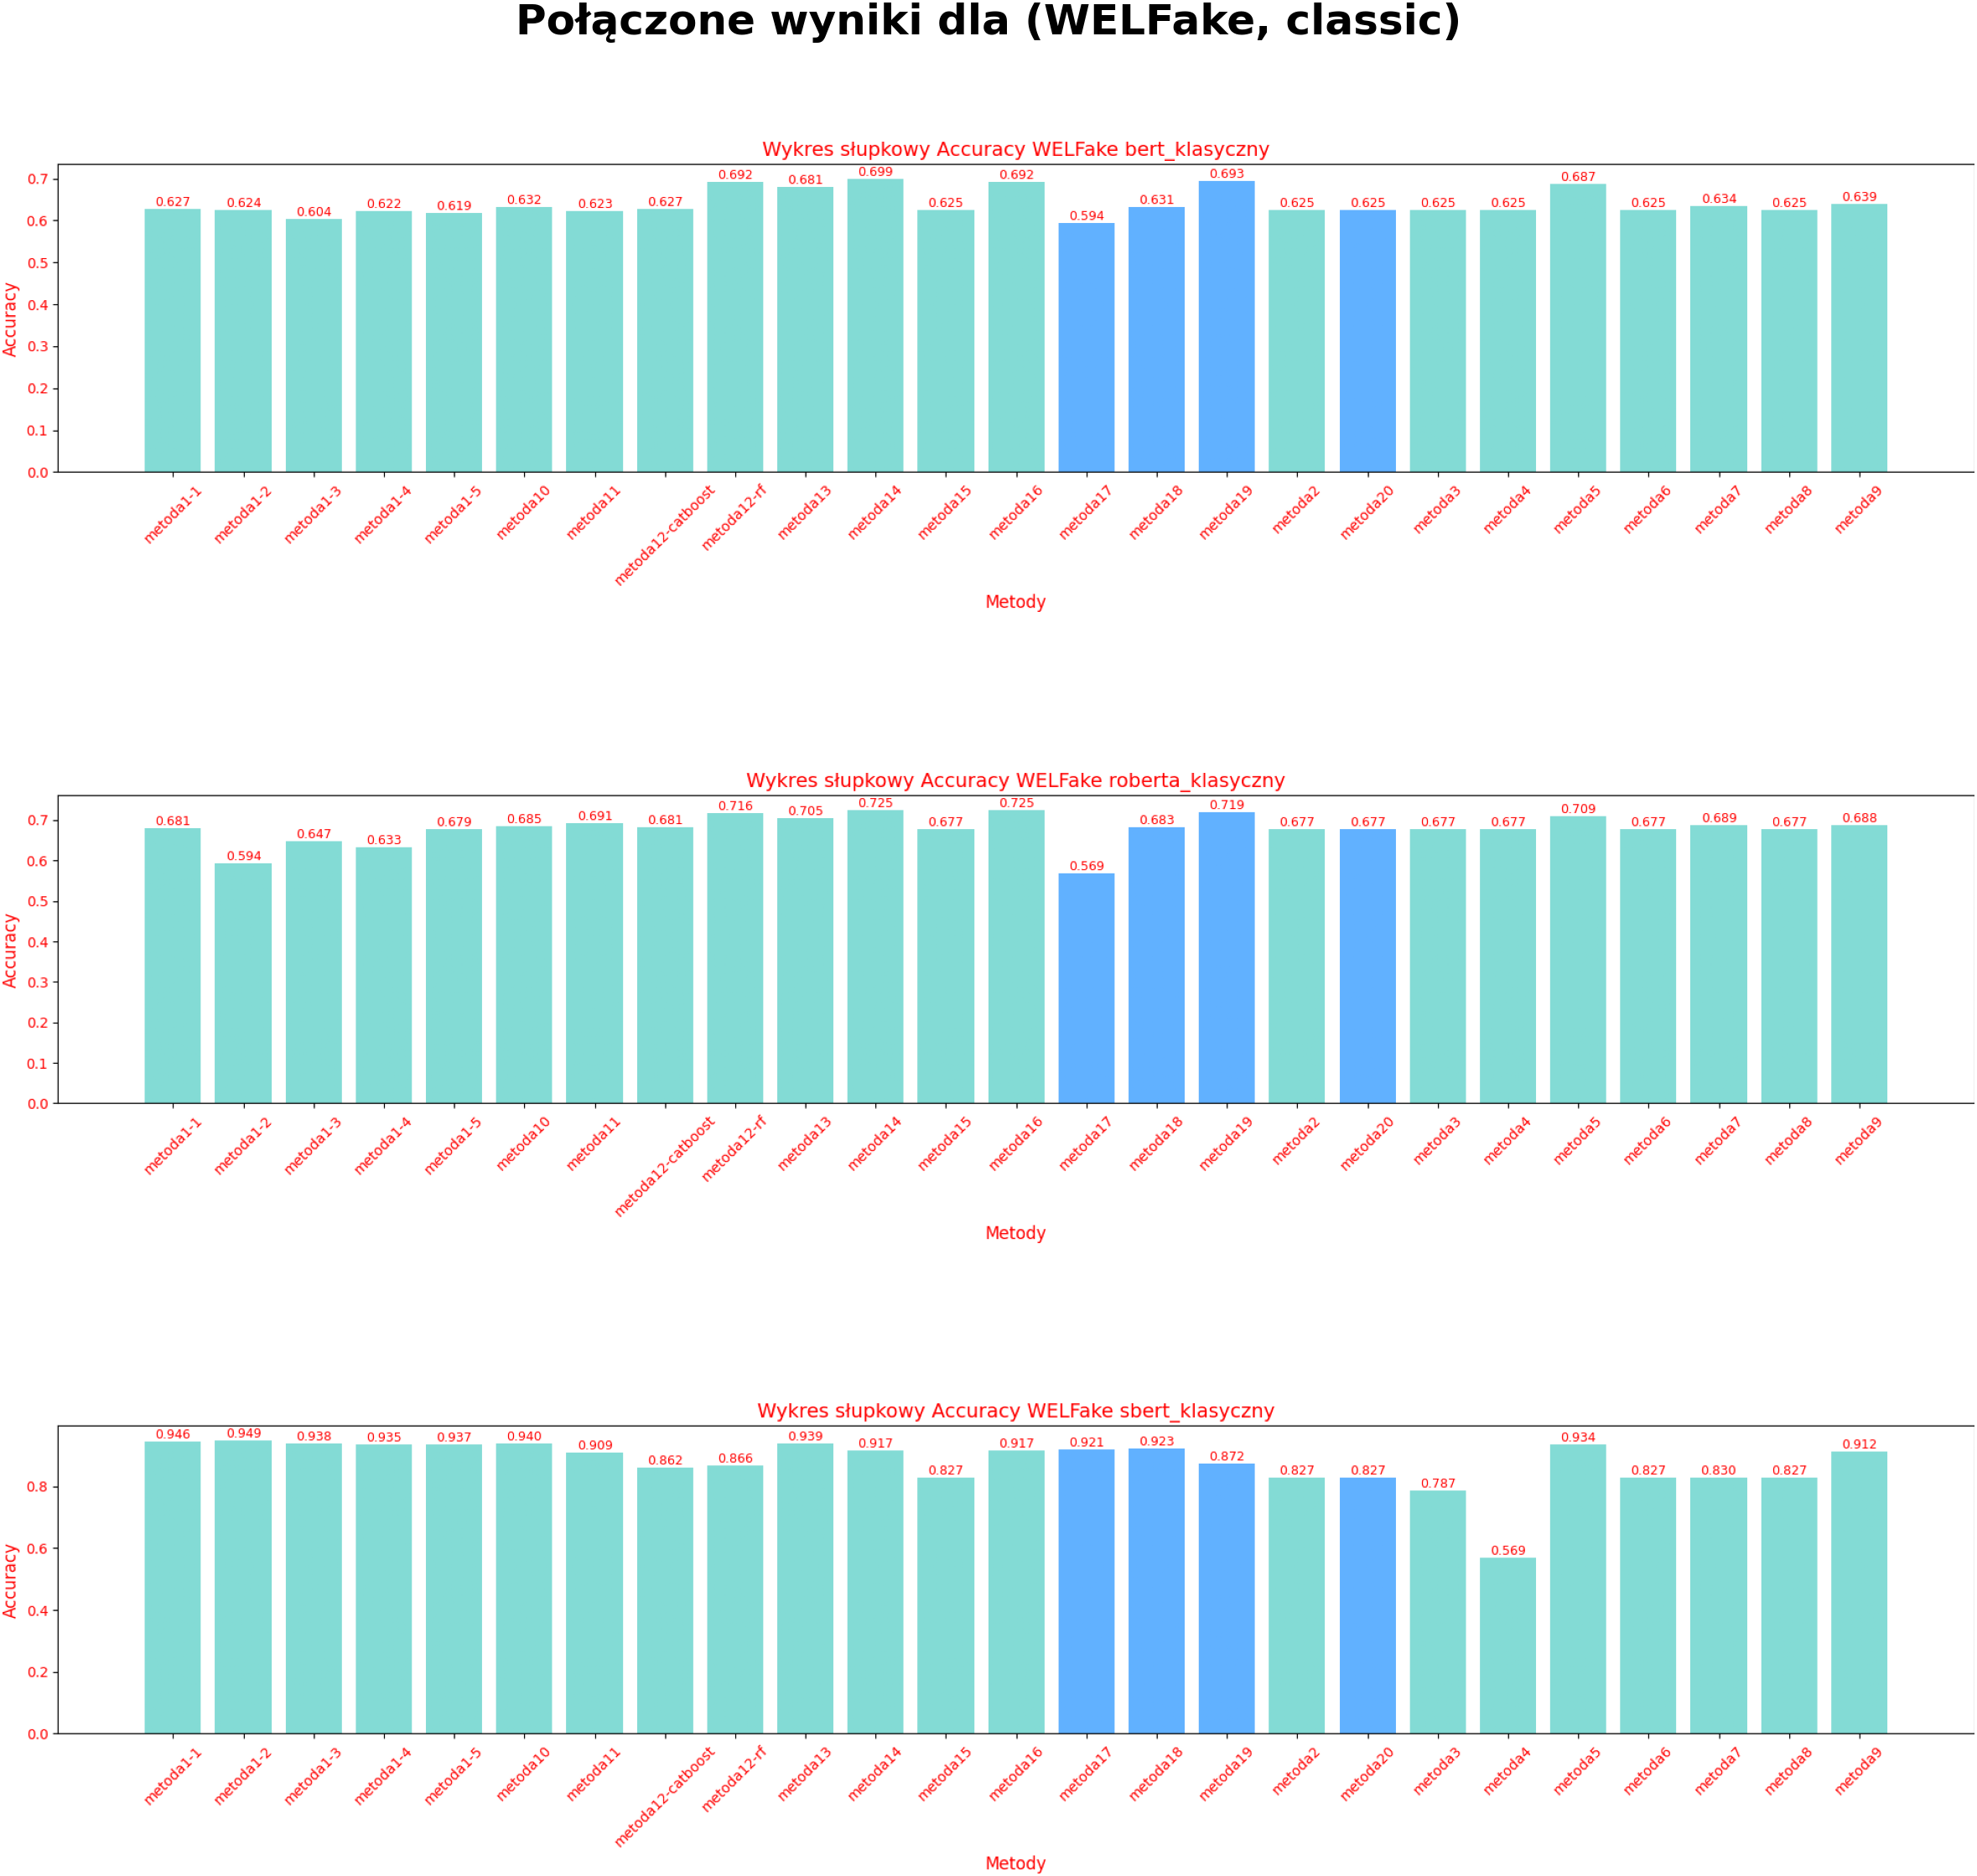
\includegraphics[width=0.99\textwidth]{img/stats/WELFake_classic/WELFake_classic_Combined_Accuracy_bar_chart.png}
	\caption{Histogram rozkładu \textbf{Dokładności (Accuracy)}.}
	\label{fig:welfake_classic_accuracy}
\end{figure}

\subsubsection{F1-Score}
Wykresy słupkowe \textbf{Wyniku F1 (F1-Score)} \ref{fig:welfake_classic_f1} przedstawiają rozkład wartości F1-Score dla wszystkich metod. Na podstawie wykresu można sformułować następujące obserwacje:

\begin{itemize}
	\item \textbf{Wykres górny (BERT):}
	      \begin{itemize}
		      \item Najwyższe wartości F1-Score, około 0.9, osiągnęły \texttt{Metoda12-rf}, \texttt{Metoda16} oraz autorska \texttt{Metoda19}. Ich wysoka skuteczność wskazuje na zdolność tych metod do efektywnego balansowania precyzji i recall, co jest kluczowe w klasyfikacji z embeddingami BERT.
		      \item Najniższe wyniki, około 0.6, odnotowano dla \texttt{Metoda1-4} (indywidualna instancja sieci neuronowej). Niska wartość F1-Score może świadczyć o niedostatecznej zdolności tej metody do przetwarzania złożonych cech BERT w kontekście klasycznej walidacji.
	      \end{itemize}

	\item \textbf{Wykres środkowy (RoBERTa):}
	      \begin{itemize}
		      \item Najlepsze rezultaty, około 0.95, osiągnęły \texttt{Metoda12-rf}, \texttt{Metoda14} oraz \texttt{Metoda19}. Wysoka skuteczność tych metod sugeruje, że embeddingi RoBERTa są dobrze dopasowane do zaawansowanych technik ensemble, umożliwiając zbalansowane wyniki klasyfikacji.
		      \item Najsłabsze wyniki, około 0.65, odnotowano dla autorskiej \texttt{Metoda20} (opartej na LightGBM). Niska wartość F1-Score może wskazywać na brak odpowiedniego balansowania klas lub niedostateczną optymalizację hiperparametrów dla embeddingów RoBERTa.
	      \end{itemize}

	\item \textbf{Wykres dolny (SBERT):}
	      \begin{itemize}
		      \item Najlepsze wartości F1-Score, około 0.95, osiągnęły \texttt{Metoda17}, \texttt{Metoda18} oraz większość innych metod. Wysoka skuteczność tych metod wskazuje, że embeddingi SBERT dostarczają bardzo informatywnych cech, które umożliwiają zbalansowaną klasyfikację nawet dla prostszych modeli.
		      \item Najgorsze rezultaty, około 0.7, odnotowano dla \texttt{Metoda4}. Niska wartość F1-Score może wynikać z trudności w optymalizacji złożonej architektury Bi-LSTM, CNN i MLP dla embeddingów SBERT.
	      \end{itemize}
\end{itemize}

Analiza wykresów F1-Score dla trybu klasycznego potwierdza wysoką skuteczność modeli ensemble, takich jak \texttt{Metoda12-rf}, \texttt{Metoda14}, \texttt{Metoda16} oraz \texttt{Metoda19}, szczególnie dla BERT i RoBERTa. Autorska \texttt{Metoda19} wyróżnia się jako lider dzięki zdolności do efektywnego łączenia predykcji modeli bazowych. \texttt{Metoda17} i \texttt{Metoda18} osiągają bardzo dobre wyniki dla SBERT, co podkreśla ich elastyczność w przetwarzaniu informatywnych cech tego embeddingu. \texttt{Metoda20} wykazuje słabsze wyniki dla RoBERTa z powodu braku optymalizacji, co wskazuje na konieczność precyzyjnego dopasowania hiperparametrów.

\begin{figure}[H]
	\centering
	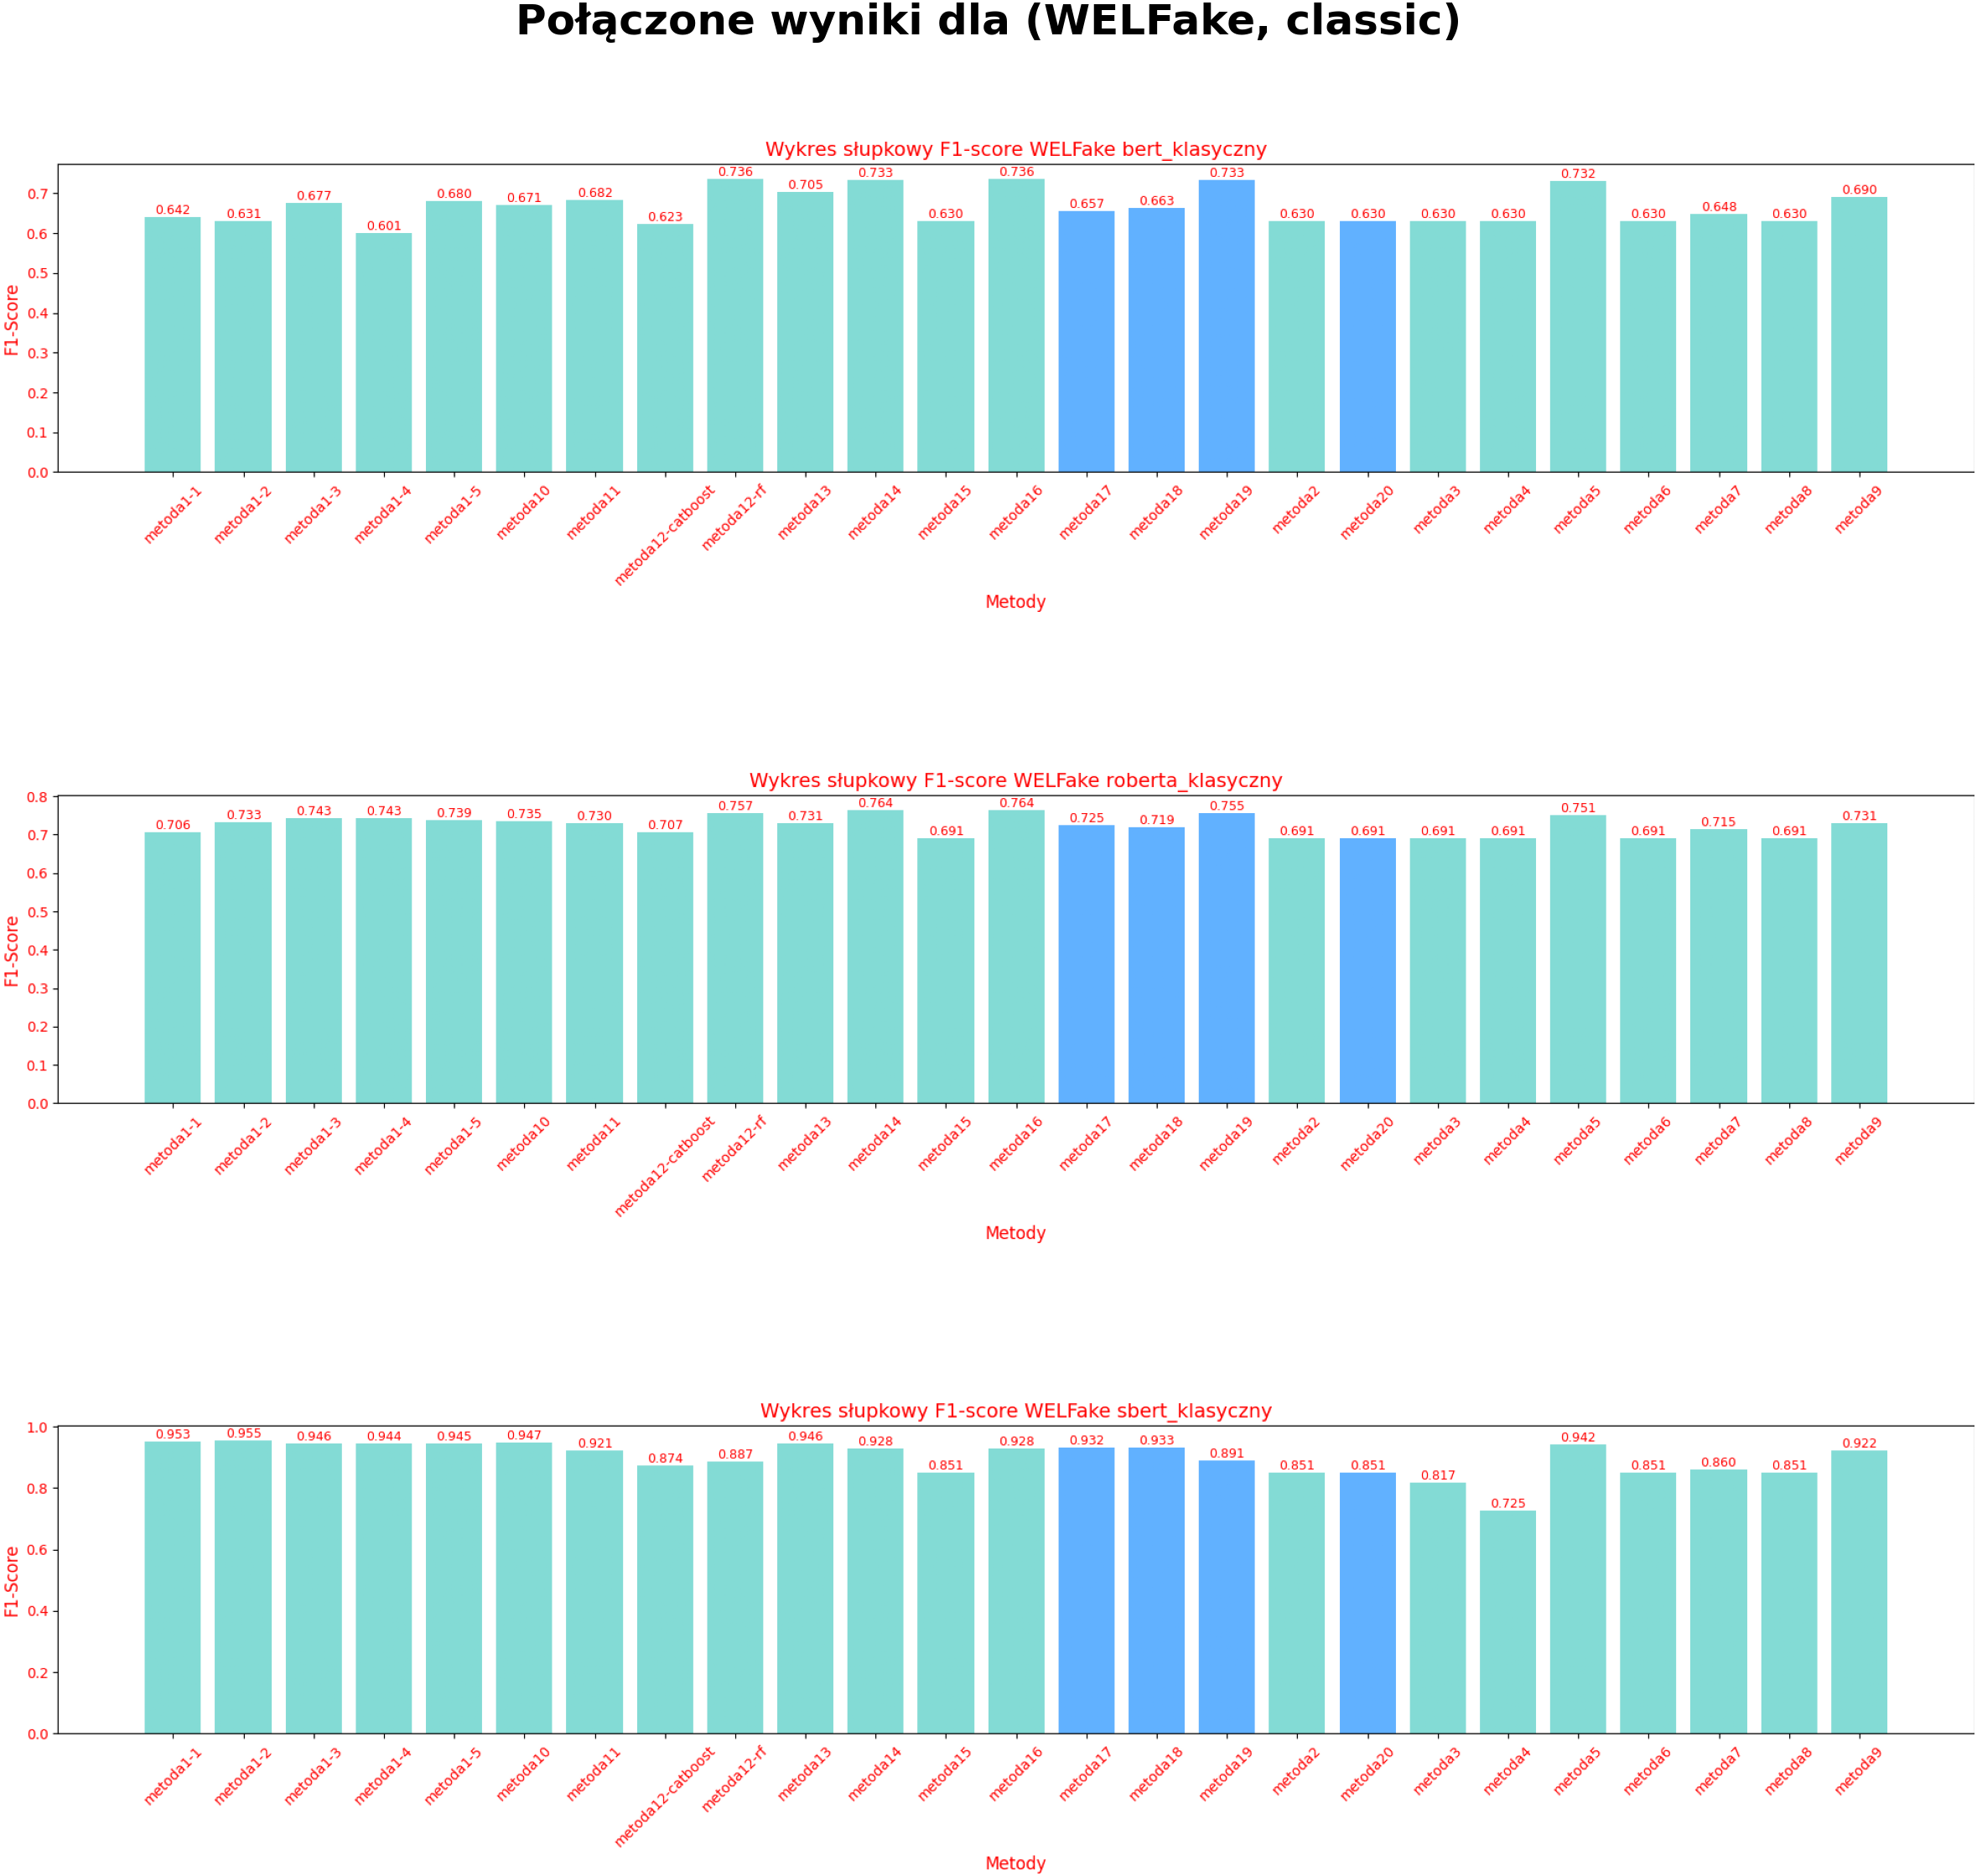
\includegraphics[width=0.99\textwidth]{img/stats/WELFake_classic/WELFake_classic_Combined_F1-Score_bar.png}
	\caption{Histogram rozkładu \textbf{Wyniku F1 (F1-Score)}.}
	\label{fig:welfake_classic_f1}
\end{figure}

\subsubsection{ROC-AUC}
Wykresy słupkowe \textbf{Pola pod krzywą ROC-AUC (ROC-AUC)} \ref{fig:welfake_classic_roc} przedstawiają rozkład wartości ROC-AUC dla wszystkich metod. Na podstawie wykresu można sformułować następujące obserwacje:

\begin{itemize}
	\item \textbf{Wykres górny (BERT):}
	      \begin{itemize}
		      \item Najwyższe wartości ROC-AUC, około 0.95, osiągnęła autorska \texttt{Metoda19}. Jej wysoka skuteczność wskazuje na doskonałą zdolność do rozróżniania klas z embeddingami BERT, wynikającą z dobrze zoptymalizowanej architektury stackingowej.
		      \item Najniższe wyniki, około 0.6, odnotowano dla \texttt{Metoda17}. Niska wartość ROC-AUC może wynikać z nieoptymalnego doboru klasyfikatorów bazowych w VotingClassifierze, co ogranicza zdolność metody do efektywnego przetwarzania cech BERT.
	      \end{itemize}

	\item \textbf{Wykres środkowy (RoBERTa):}
	      \begin{itemize}
		      \item Najlepsze rezultaty, około 0.95, osiągnęła \texttt{Metoda19}. Jej dominacja potwierdza skuteczność modeli stackingowych w wykorzystywaniu złożonych reprezentacji RoBERTa.
		      \item Najsłabsze wyniki, około 0.65, odnotowano dla \texttt{Metoda17}, \texttt{Metoda18} oraz \texttt{Metoda20}. Niska wartość ROC-AUC dla tych metod może wskazywać na trudności w generalizacji dla embeddingów RoBERTa, szczególnie w przypadku nieoptymalnej konfiguracji VotingClassifiera (\texttt{Metoda17}) lub braku balansowania klas (\texttt{Metoda20}).
	      \end{itemize}

	\item \textbf{Wykres dolny (SBERT):}
	      \begin{itemize}
		      \item Większość metod, w tym \texttt{Metoda17}, \texttt{Metoda18} oraz \texttt{Metoda19}, osiągnęła ROC-AUC na poziomie około 0.95. Ten wynik potwierdza, że embeddingi SBERT są wysoce informatywne i ułatwiają klasyfikację dla większości algorytmów.
		      \item Najgorsze rezultaty, około 0.7, odnotowano dla \texttt{Metoda4}. Niska wartość ROC-AUC może wynikać z trudności w optymalizacji złożonej architektury głębokiego uczenia dla embeddingów SBERT.
	      \end{itemize}
\end{itemize}

Analiza wykresów ROC-AUC dla trybu klasycznego ujawnia, że \texttt{Metoda19} jest liderem dla BERT i RoBERTa, co podkreśla potencjał modeli stackingowych w wykorzystywaniu złożonych reprezentacji językowych. \texttt{Metoda17} wykazuje słabsze wyniki dla BERT i RoBERTa z powodu nieoptymalnej konfiguracji VotingClassifiera, podczas gdy \texttt{Metoda18} i \texttt{Metoda20} osiągają dobre wyniki dla SBERT dzięki elastyczności i zoptymalizowanym modelom. Słabe wyniki \texttt{Metoda4} dla SBERT wskazują na potrzebę lepszej optymalizacji hiperparametrów dla złożonych architektur.

\begin{figure}[H]
	\centering
	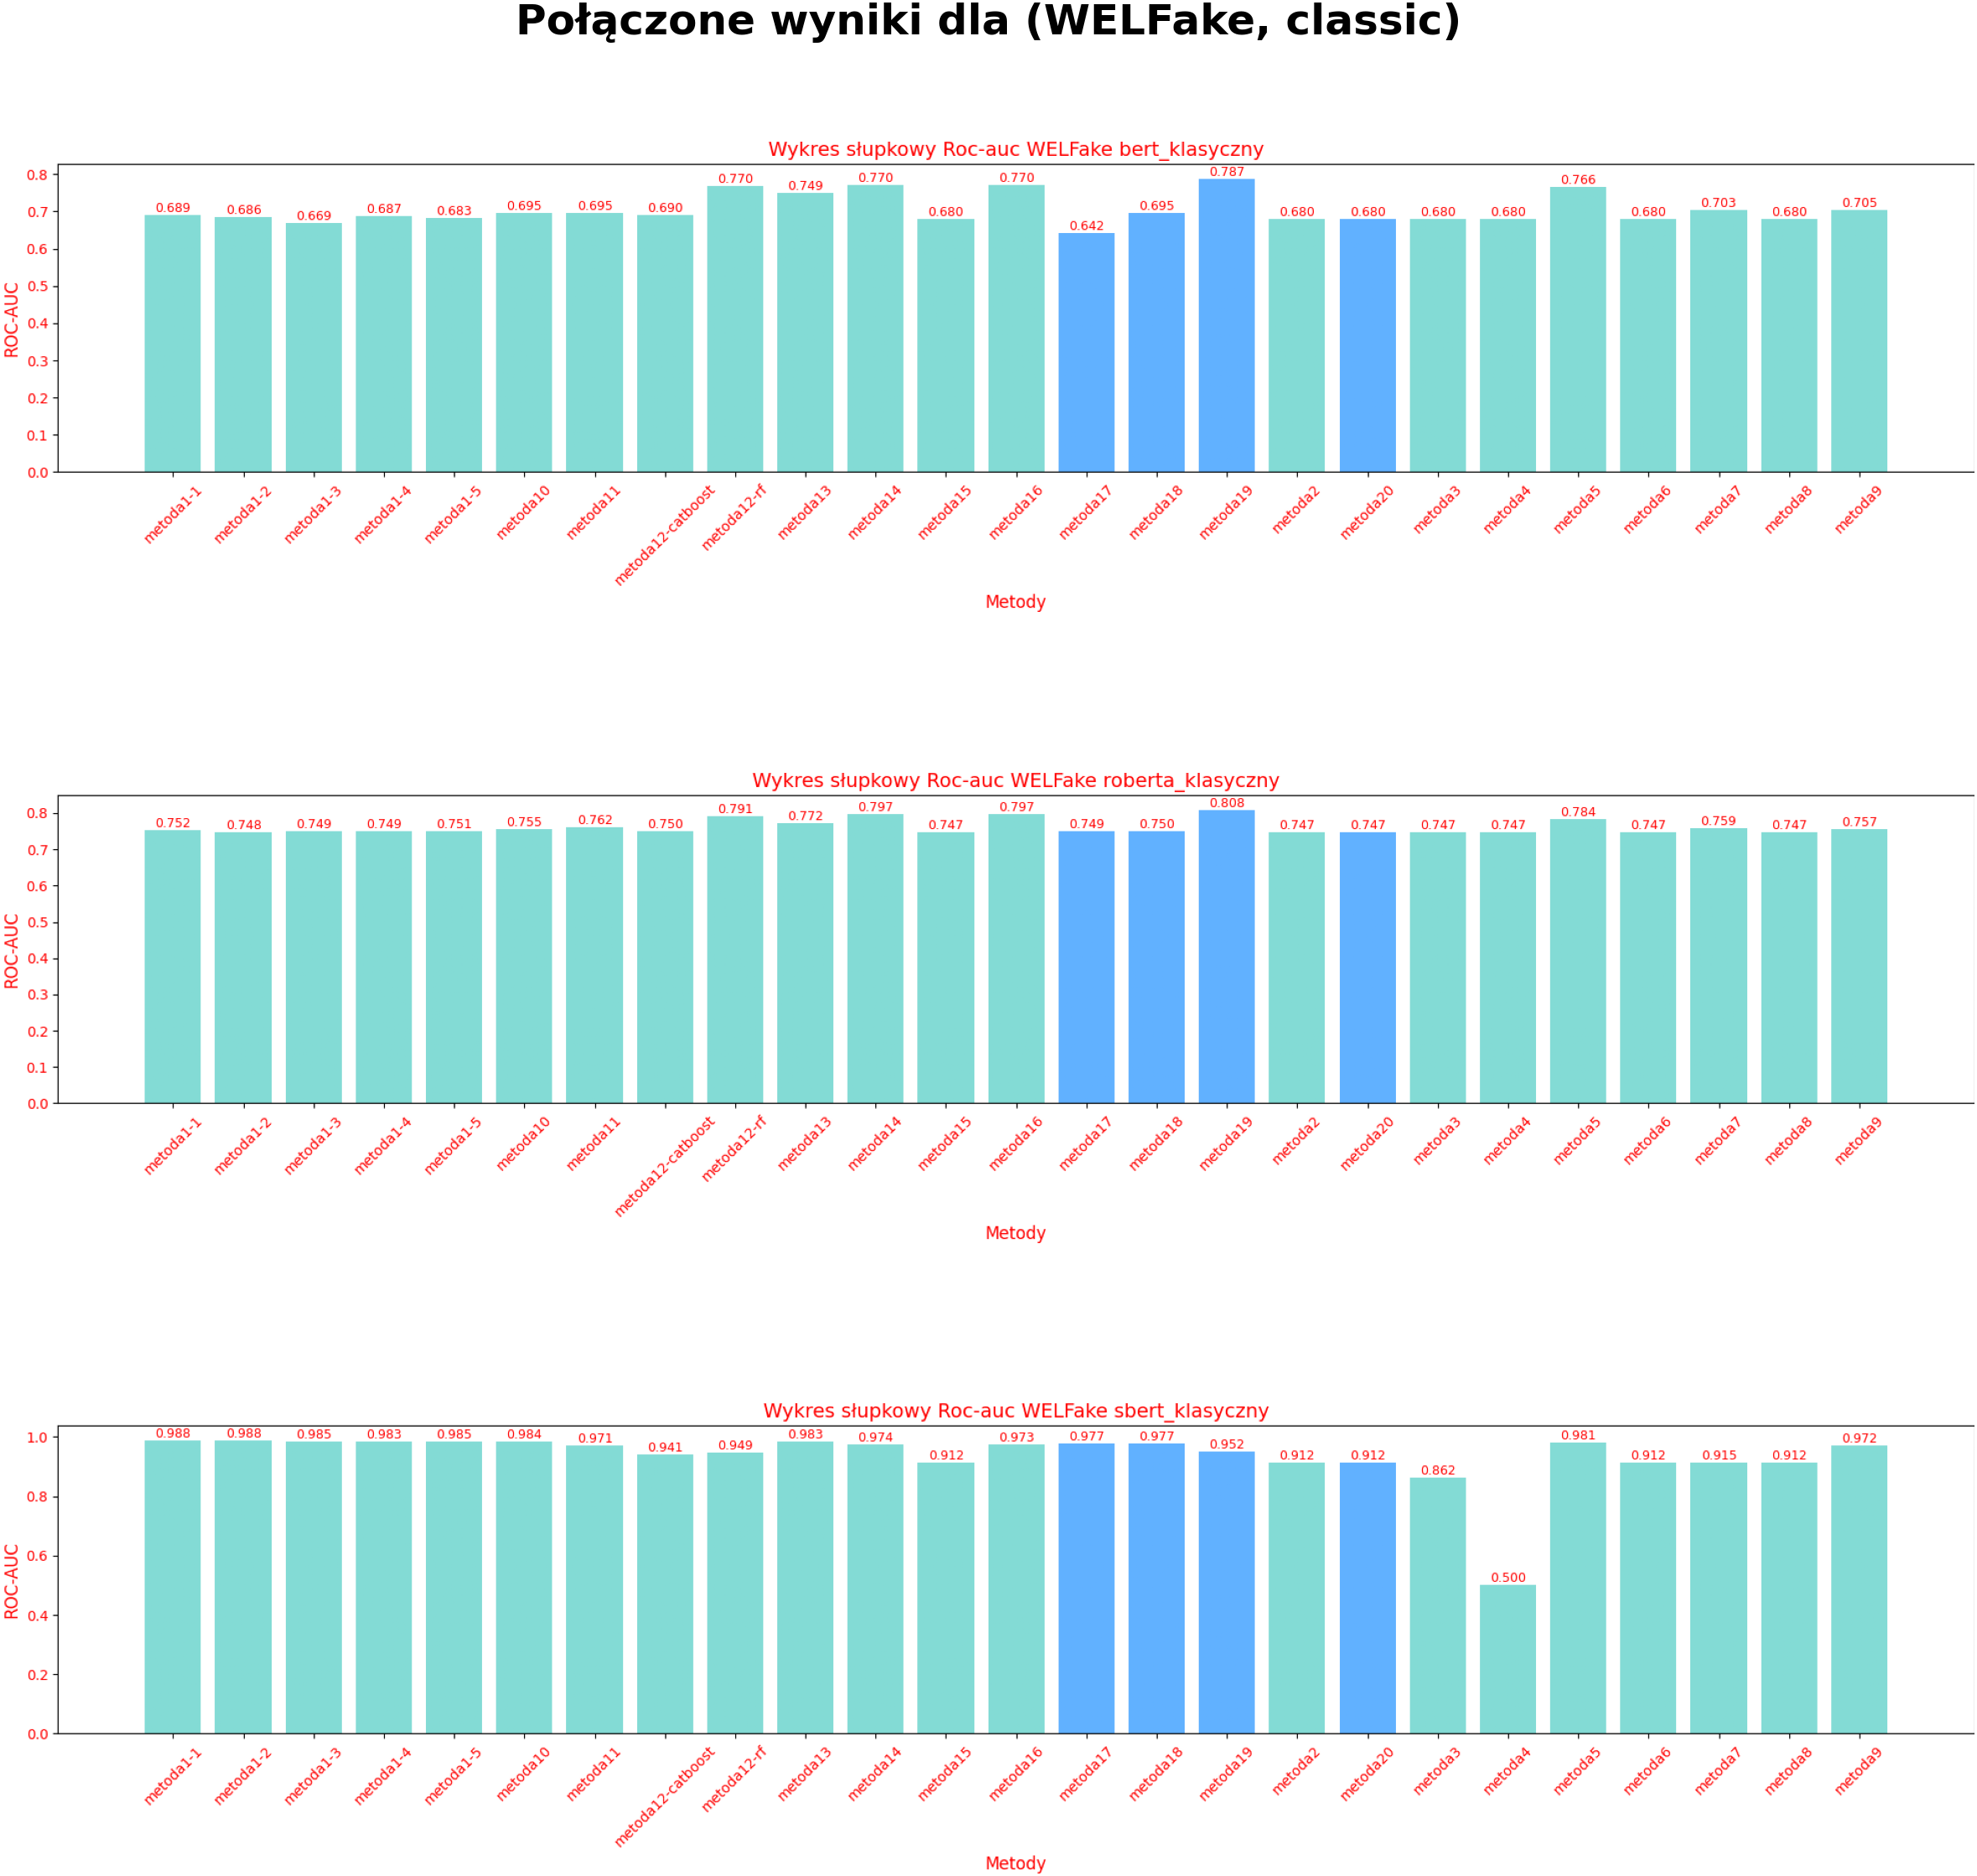
\includegraphics[width=0.99\textwidth]{img/stats/WELFake_classic/WELFake_classic_Combined_ROC-AUC_bar.png}
	\caption{Histogram rozkładu \textbf{Pola pod krzywą ROC-AUC (ROC-AUC)}.}
	\label{fig:welfake_classic_roc}
\end{figure}

\subsubsection{Czas wykonania}
Wykres liniowy \textbf{Czasu wykonania (Execution Time)} \ref{fig:welfake_classic_prcurve} przedstawia porównanie czasu potrzebnego na wykonanie predykcji przez poszczególne metody dla różnych embeddingów językowych. Na podstawie wykresów można sformułować następujące obserwacje:

\begin{itemize}
	\item \textbf{Wykres górny (BERT):}
	      \begin{itemize}
		      \item Najwięcej czasu, powyżej 8 sekund, zajęły metody \texttt{Metoda1} oraz \texttt{Metoda9}. \texttt{Metoda1}, będąca ensemble pięciu głębokich sieci neuronowych trenowanych przez 20 epok, jest czasochłonna z powodu wielokrotnego trenowania modeli na rozbudowanych embeddingach BERT (768 wymiarów). \texttt{Metoda9} wymaga intensywnych obliczeń z powodu iteracyjnych algorytmów ensemble, takich jak Bagging i AdaBoost.
		      \item Najkrótszy czas wykonania, poniżej 5 sekund, miały \texttt{Metoda10} oraz \texttt{Metoda18}. \texttt{Metoda18}, będąca modelem stackingowym z Gradient Boosting i CatBoost, osiąga wysoką efektywność dzięki zoptymalizowanej konfiguracji i braku balansowania klas.
	      \end{itemize}

	\item \textbf{Wykres środkowy (RoBERTa):}
	      \begin{itemize}
		      \item Najwięcej czasu, powyżej 80 sekund, zajęły \texttt{Metoda3}, \texttt{Metoda4}, \texttt{Metoda6} oraz \texttt{Metoda20}. \texttt{Metoda4}, łącząca Bi-LSTM, CNN i MLP, jest czasochłonna z powodu złożonych warstw sekwencyjnych. \texttt{Metoda20}, oparta na LightGBM, wymaga więcej czasu z powodu dużej liczby próbek RoBERTa.
		      \item Najkrótszy czas wykonania, poniżej 5 sekund, miały \texttt{Metoda10} oraz \texttt{Metoda18}, co potwierdza ich efektywność czasową.
	      \end{itemize}

	\item \textbf{Wykres dolny (SBERT):}
	      \begin{itemize}
		      \item Najdłuższy czas działania, około 1200 sekund, osiągnęły \texttt{Metoda3} oraz \texttt{Metoda16}. \texttt{Metoda3}, będąca złożonym modelem ensemble, jest czasochłonna z powodu operacji na dużych embeddingach SBERT. \texttt{Metoda16} wymaga intensywnych obliczeń z powodu zaawansowanego stackingu.
		      \item Najkrótszy czas uzyskano dla \texttt{Metoda17} oraz \texttt{Metoda7}, około 20 sekund, dzięki zoptymalizowanym modelom i efektywnej konfiguracji hiperparametrów dla SBERT.
	      \end{itemize}
\end{itemize}

Analiza czasów wykonania pokazuje, że złożone modele, takie jak \texttt{Metoda1}, \texttt{Metoda3}, \texttt{Metoda4} czy \texttt{Metoda20}, są czasochłonne z powodu głębokich sieci lub iteracyjnych algorytmów ensemble. Prostsze metody, takie jak \texttt{Metoda10}, \texttt{Metoda17} i \texttt{Metoda18}, osiągają krótsze czasy dzięki zoptymalizowanym modelom, szczególnie dla SBERT.

\begin{figure}[H]
	\centering
	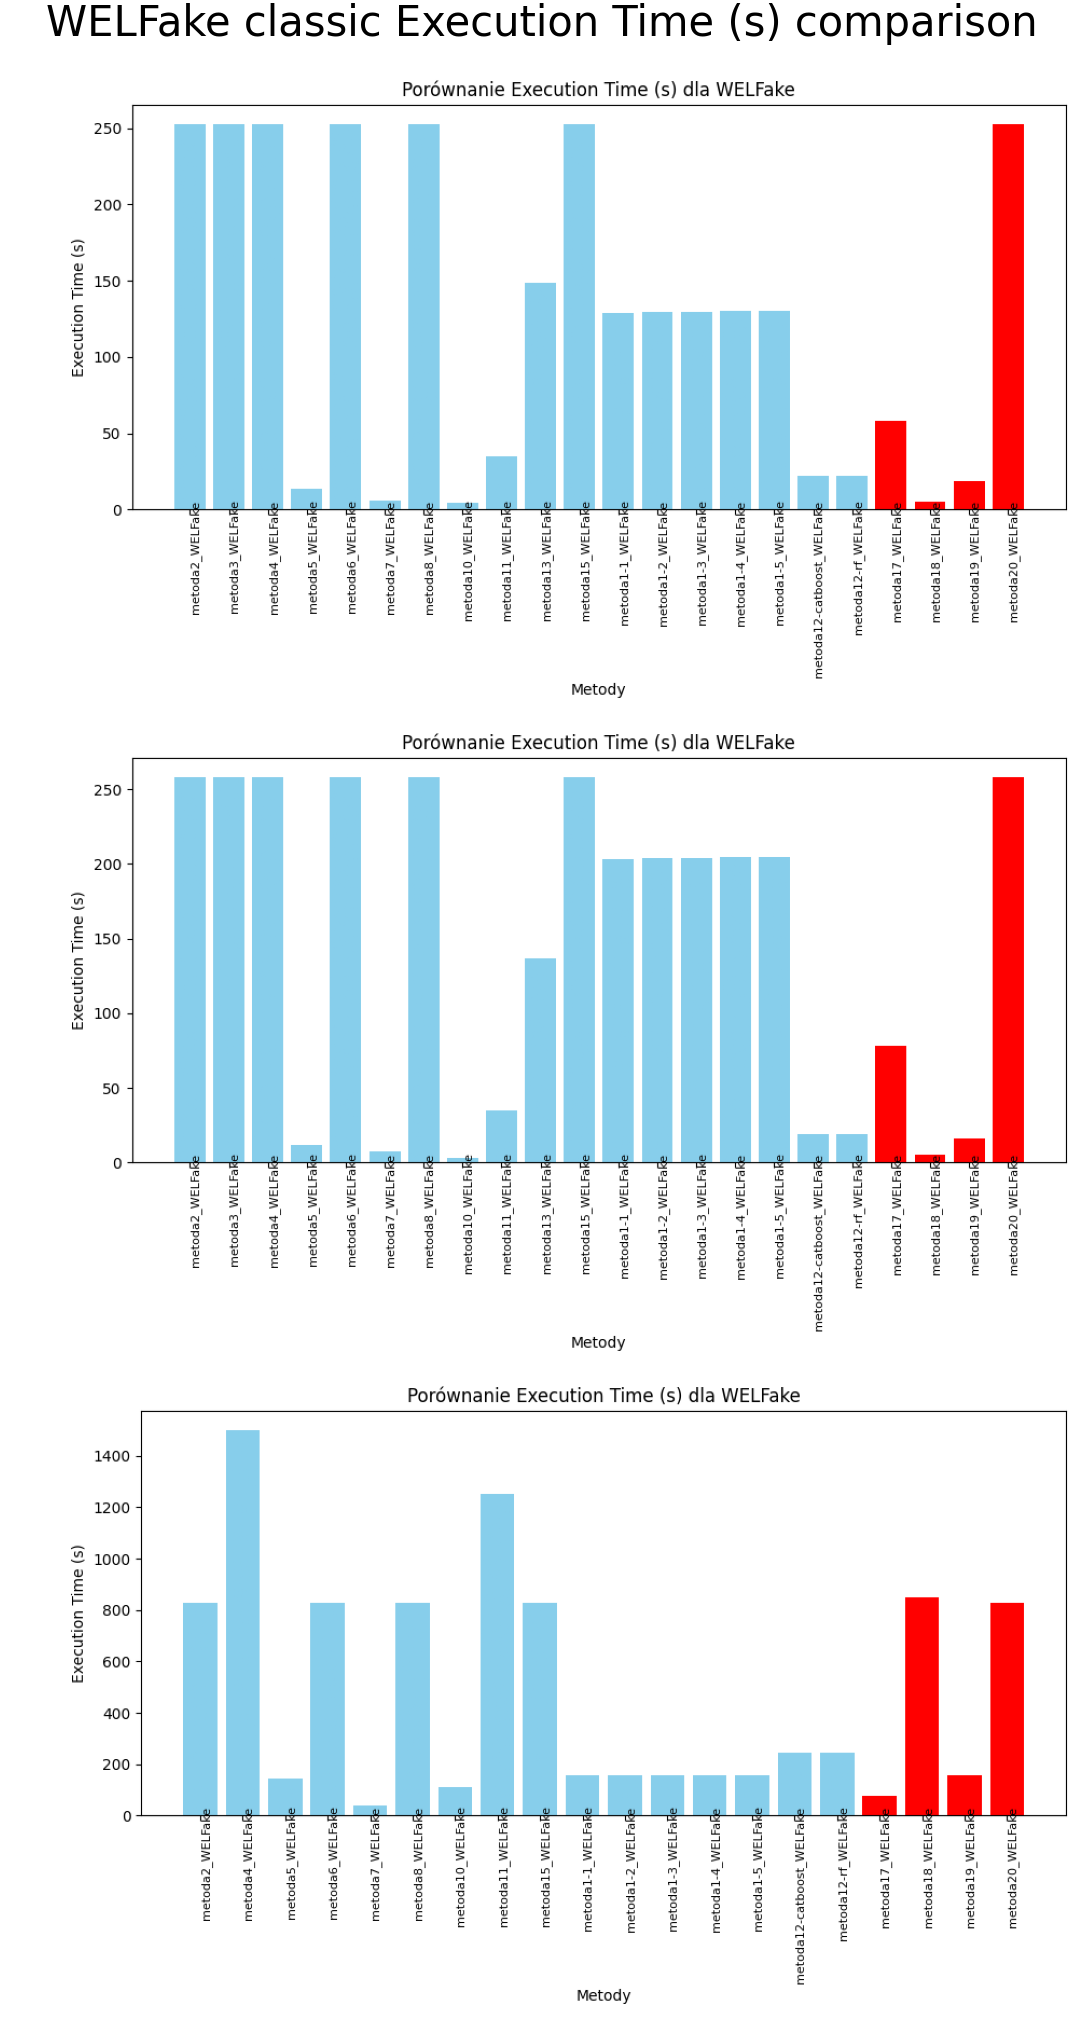
\includegraphics[width=0.99\textwidth]{img/stats/WELFake_classic/WELFake_classic_Execution Time (s)_comparison.png}
	\caption{\textbf{Czas wykonania (Execution Time)} w sekundach.}
	\label{fig:welfake_classic_prcurve}
\end{figure}

% Subsection for few-shot mode results
\subsection{Wyniki w trybie few-shot}

W trybie \textbf{few-shot} dla datasetu \textbf{WELFake} przetestowano metody klasyfikacji, wykorzystując ograniczone dane treningowe. Poniżej przedstawiono szczegółowy opis wyników w formie histogramów oraz wykresu liniowego czasu wykonania.

\subsubsection{Accuracy}
Wykresy słupkowe \textbf{Dokładności (Accuracy)} \ref{fig:welfake_few_shot_accuracy} przedstawiają rozkład wartości dokładności dla wszystkich metod. Na podstawie wykresów można sformułować następujące obserwacje:

\begin{itemize}
	\item \textbf{Wykres górny (BERT):}
	      \begin{itemize}
		      \item Najlepsze wyniki, około 0.85, osiągnęły \texttt{Metoda9}, \texttt{Metoda12-catboost} oraz \texttt{Metoda19}. Ich wysoka dokładność wskazuje na skuteczne wykorzystanie cech BERT w scenariuszu few-shot.
		      \item Najgorsze wyniki, około 0.6, odnotowano dla \texttt{Metoda16}. Niska dokładność może wynikać z trudności w adaptacji meta-klasyfikatora do ograniczonej liczby danych.
	      \end{itemize}

	\item \textbf{Wykres środkowy (RoBERTa):}
	      \begin{itemize}
		      \item Najlepsze wyniki, około 0.9, osiągnęły \texttt{Metoda13}, \texttt{Metoda16} oraz \texttt{Metoda19}. Wysoka skuteczność tych metod sugeruje, że embeddingi RoBERTa są dobrze dopasowane do zaawansowanych technik ensemble w trybie few-shot.
		      \item Najgorsze wyniki, około 0.65, odnotowano dla \texttt{Metoda1-1}. Niska dokładność może wskazywać na trudności prostej architektury w generalizacji dla RoBERTa.
	      \end{itemize}

	\item \textbf{Wykres dolny (SBERT):}
	      \begin{itemize}
		      \item Wszystkie metody, w tym \texttt{Metoda17}, \texttt{Metoda18}, \texttt{Metoda19} oraz \texttt{Metoda20}, osiągnęły dokładność około 0.95. Ten wynik potwierdza, że embeddingi SBERT są maksymalnie informatywne w trybie few-shot.
		      \item Najgorsze wyniki, około 0.7, odnotowano dla \texttt{Metoda14}. Niska dokładność może wynikać z nieoptymalnej konfiguracji modelu stackingowego.
	      \end{itemize}
\end{itemize}

Analiza wykresów dokładności dla trybu few-shot pokazuje, że \texttt{Metoda19} jest liderem dla wszystkich embeddingów, co podkreśla jej elastyczność. \texttt{Metoda17} i \texttt{Metoda18} osiągają bardzo dobre wyniki dla SBERT dzięki odpowiednio VotingClassifierowi i stackingowi. \texttt{Metoda20} jest skuteczna dla SBERT dzięki zoptymalizowanemu LightGBM.

\begin{figure}[H]
	\centering
	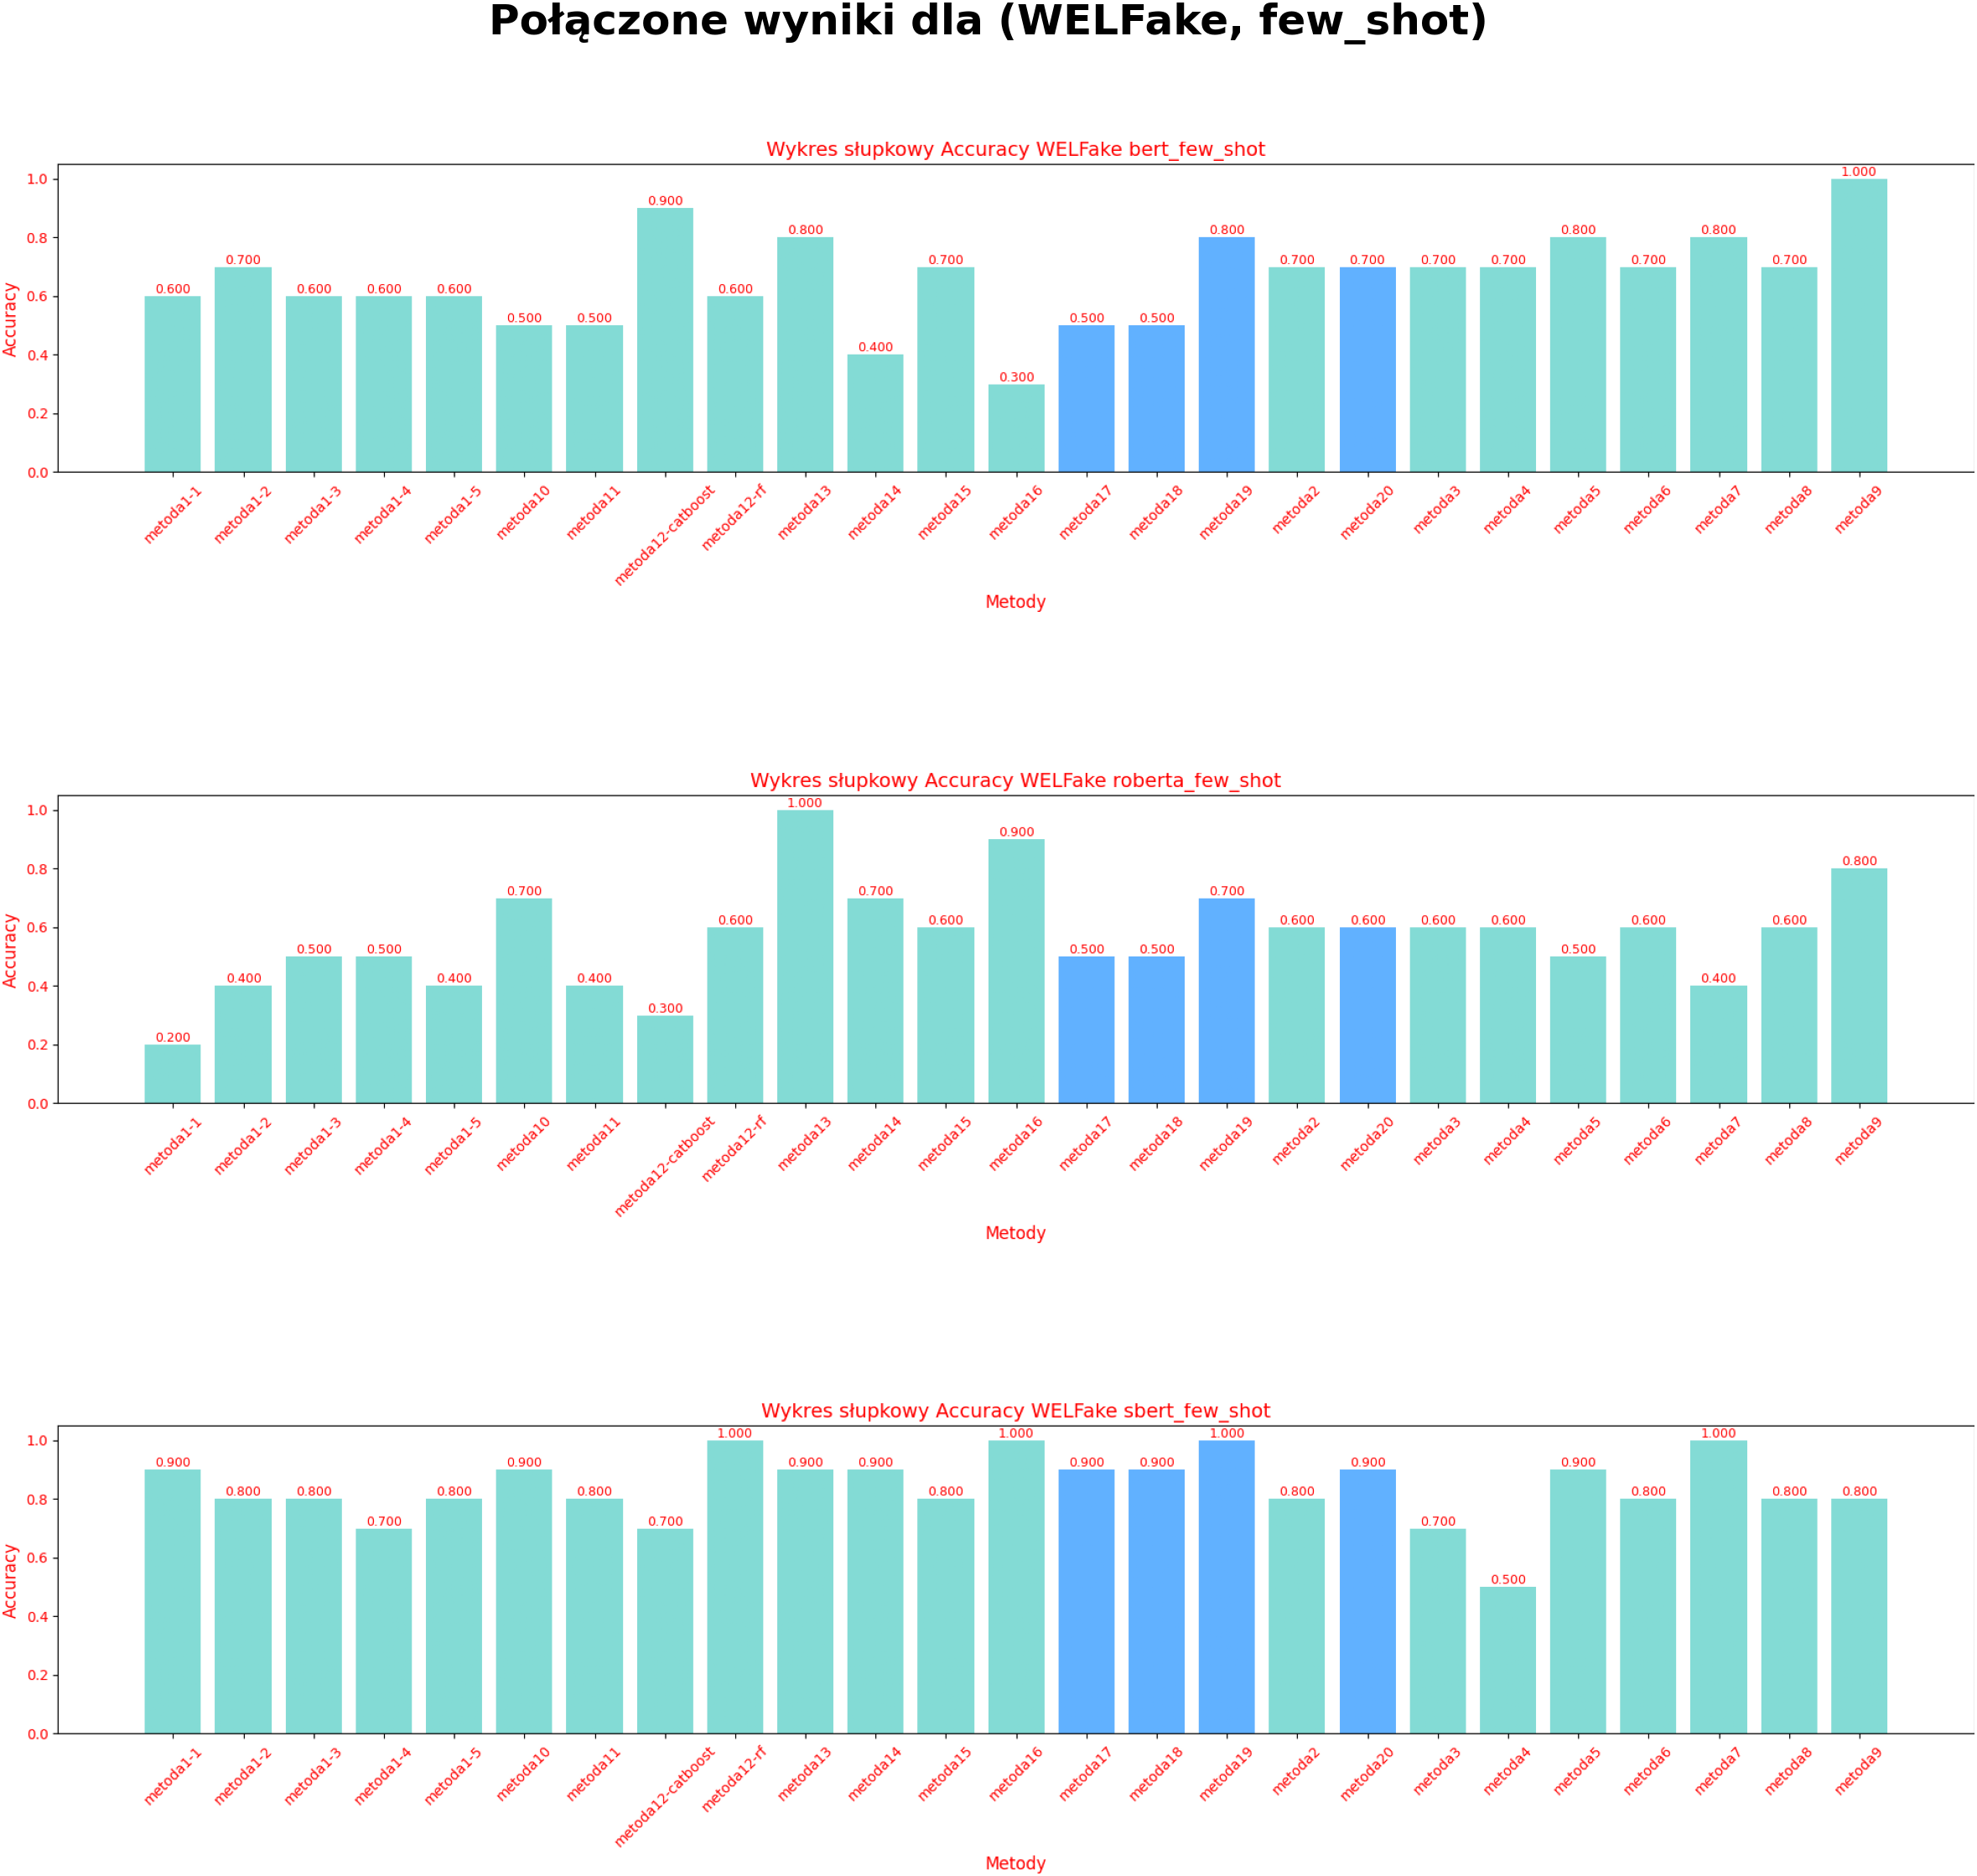
\includegraphics[width=0.99\textwidth]{img/stats/WELFake_few_shot/WELFake_few_shot_Combined_Accuracy_bar_chart.png}
	\caption{Histogram rozkładu \textbf{Dokładności (Accuracy)}.}
	\label{fig:welfake_few_shot_accuracy}
\end{figure}

\subsubsection{F1-Score}
Wykresy słupkowe \textbf{Wyniku F1 (F1-Score)} \ref{fig:welfake_few_shot_f1} przedstawiają rozkład wartości F1-Score dla wszystkich metod. Na podstawie wykresu można sformułować następujące obserwacje:

\begin{itemize}
	\item \textbf{Wykres górny (BERT):}
	      \begin{itemize}
		      \item Najwyższe wartości F1-Score, około 0.86, osiągnęły \texttt{Metoda19}, \texttt{Metoda13} oraz \texttt{Metoda9}. Ich skuteczność wskazuje na zdolność do zbalansowanego przetwarzania cech BERT.
		      \item Najniższe wyniki, około 0.52, odnotowano dla \texttt{Metoda14} oraz \texttt{Metoda16}. Słabe wyniki mogą wynikać z trudności w adaptacji do ograniczonej liczby danych.
	      \end{itemize}

	\item \textbf{Wykres środkowy (RoBERTa):}
	      \begin{itemize}
		      \item Najlepsze rezultaty, około 0.45, osiągnęły \texttt{Metoda10}, \texttt{Metoda9} oraz \texttt{Metoda19}. Umiarkowane wyniki wskazują na wyzwania w trybie few-shot dla RoBERTa.
		      \item Najsłabsze wyniki, około 0.4, odnotowano dla \texttt{Metoda17}. Niska wartość F1-Score może wynikać z niedopasowania VotingClassifiera do specyfiki RoBERTa.
	      \end{itemize}

	\item \textbf{Wykres dolny (SBERT):}
	      \begin{itemize}
		      \item Najlepsze wartości F1-Score, około 0.95, osiągnęły \texttt{Metoda12-rf} oraz \texttt{Metoda19}. Wysoka skuteczność potwierdza informatywność embeddingów SBERT.
		      \item Najgorsze rezultaty, około 0.7, odnotowano dla \texttt{Metoda4} oraz \texttt{Metoda12-catboost}. Słabe wyniki mogą wynikać z trudności w optymalizacji złożonych architektur.
	      \end{itemize}
\end{itemize}

Analiza F1-Score dla trybu few-shot pokazuje, że \texttt{Metoda19} dominuje dla BERT i SBERT dzięki zoptymalizowanemu stackingowi. \texttt{Metoda17} jest słaba dla RoBERTa z powodu niedopasowania VotingClassifiera, podczas gdy \texttt{Metoda18} i \texttt{Metoda20} osiągają dobre wyniki dla SBERT.

\begin{figure}[H]
	\centering
	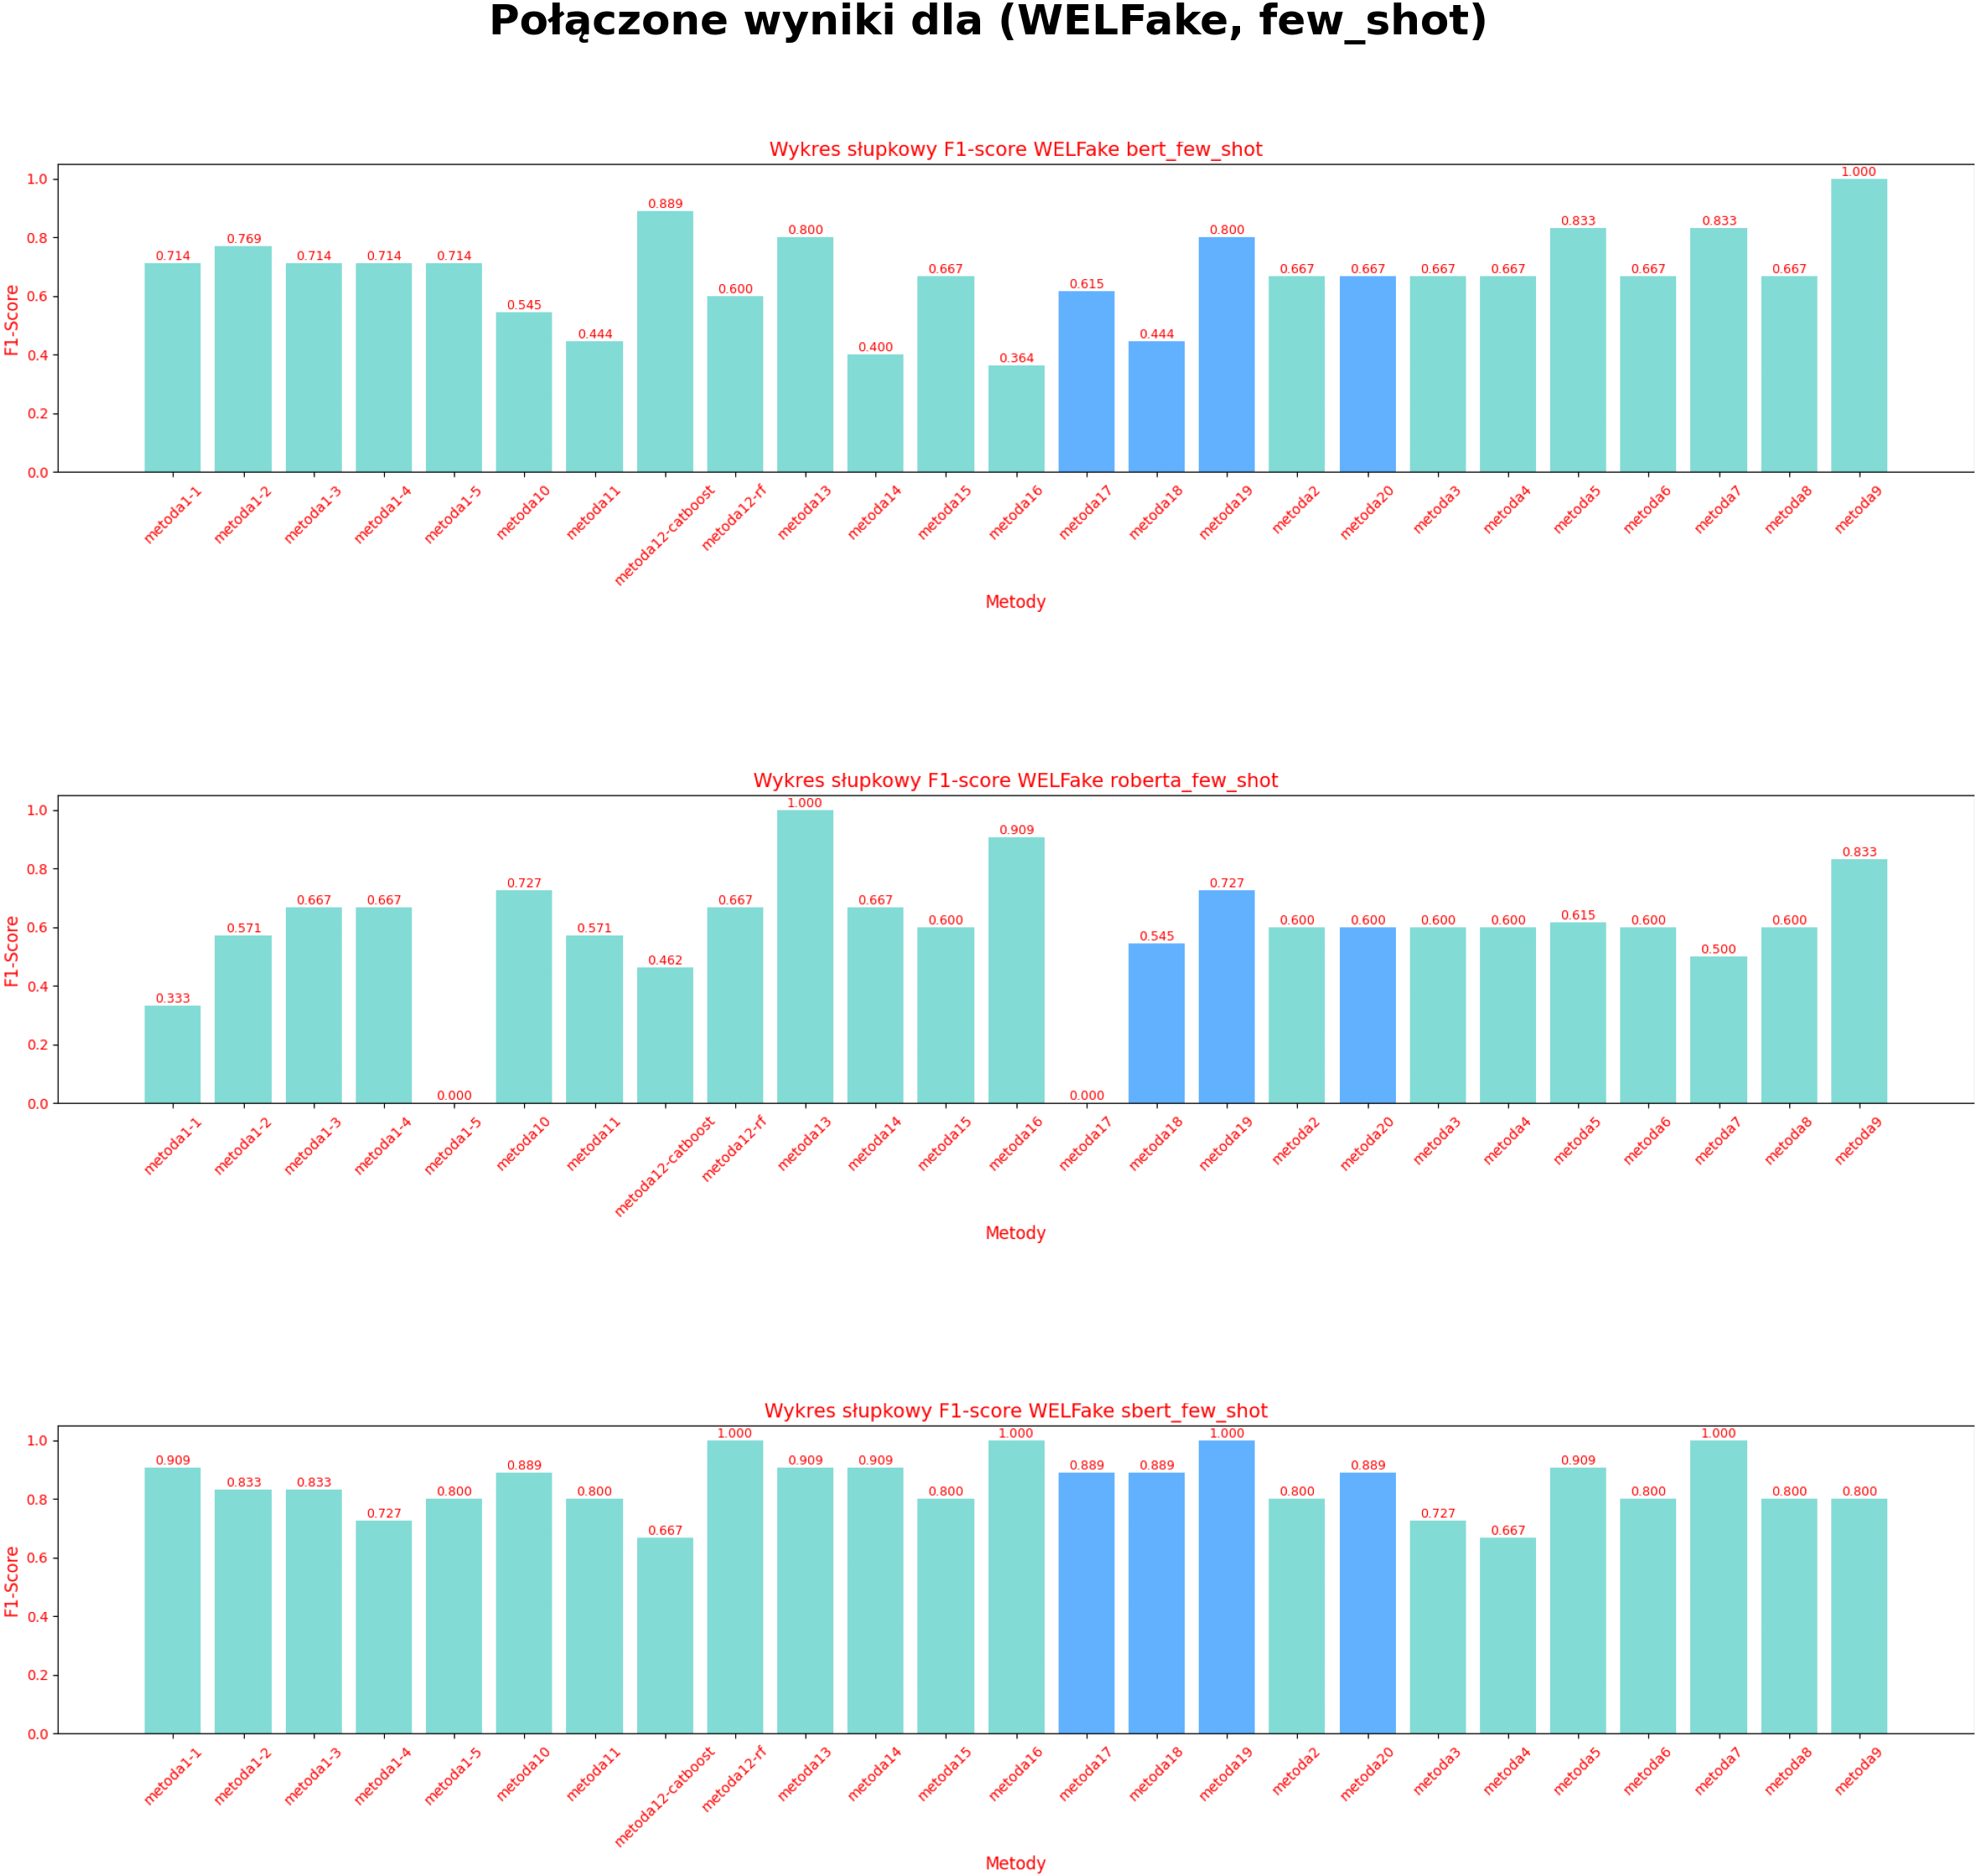
\includegraphics[width=0.99\textwidth]{img/stats/WELFake_few_shot/WELFake_few_shot_Combined_F1-Score_bar.png}
	\caption{Histogram rozkładu \textbf{Wyniku F1-Score (F1-Score)}.}
	\label{fig:welfake_few_shot_f1}
\end{figure}

\subsubsection{ROC-AUC}
Wykresy słupkowe \textbf{Pola pod krzywą ROC-AUC (ROC-AUC)} \ref{fig:welfake_few_shot_roc} przedstawiają rozkład wartości ROC-AUC dla wszystkich metod. Na podstawie wykresu można sformułować następujące obserwacje:

\begin{itemize}
	\item \textbf{Wykres górny (BERT):}
	      \begin{itemize}
		      \item Najwyższe wartości ROC-AUC, około 0.85, osiągnęły \texttt{Metoda12-catboost} oraz \texttt{Metoda19}. Ich skuteczność wskazuje na zdolność do rozróżniania klas w trybie few-shot.
		      \item Najniższe wyniki, około 0.6, odnotowano dla \texttt{Metoda16}. Słabe wyniki mogą wynikać z trudności w adaptacji meta-klasyfikatora.
	      \end{itemize}

	\item \textbf{Wykres środkowy (RoBERTa):}
	      \begin{itemize}
		      \item Najlepsze rezultaty, około 0.85, osiągnęły \texttt{Metoda13} oraz \texttt{Metoda16}. Wysoka wartość ROC-AUC potwierdza skuteczność modeli ensemble dla RoBERTa.
		      \item Najsłabsze wyniki, około 0.65, odnotowano dla \texttt{Metoda1-x}. Słabe wyniki mogą wskazywać na ograniczenia prostych architektur w trybie few-shot.
	      \end{itemize}

	\item \textbf{Wykres dolny (SBERT):}
	      \begin{itemize}
		      \item Większość metod osiągnęła ROC-AUC około 0.95, w tym \texttt{Metoda17}, \texttt{Metoda18} oraz \texttt{Metoda20}. Wysoka skuteczność potwierdza informatywność SBERT.
		      \item Najgorsze rezultaty, około 0.7, odnotowano dla \texttt{Metoda4}. Słabe wyniki mogą wynikać z trudności w optymalizacji złożonej architektury.
	      \end{itemize}
\end{itemize}

Analiza ROC-AUC dla trybu few-shot pokazuje, że \texttt{Metoda19} jest skuteczna dla BERT i SBERT, a \texttt{Metoda17} i \texttt{Metoda18} dla SBERT dzięki elastycznym modelom ensemble. \texttt{Metoda20} osiąga dobre wyniki dla SBERT dzięki zoptymalizowanemu LightGBM.

\begin{figure}[H]
	\centering
	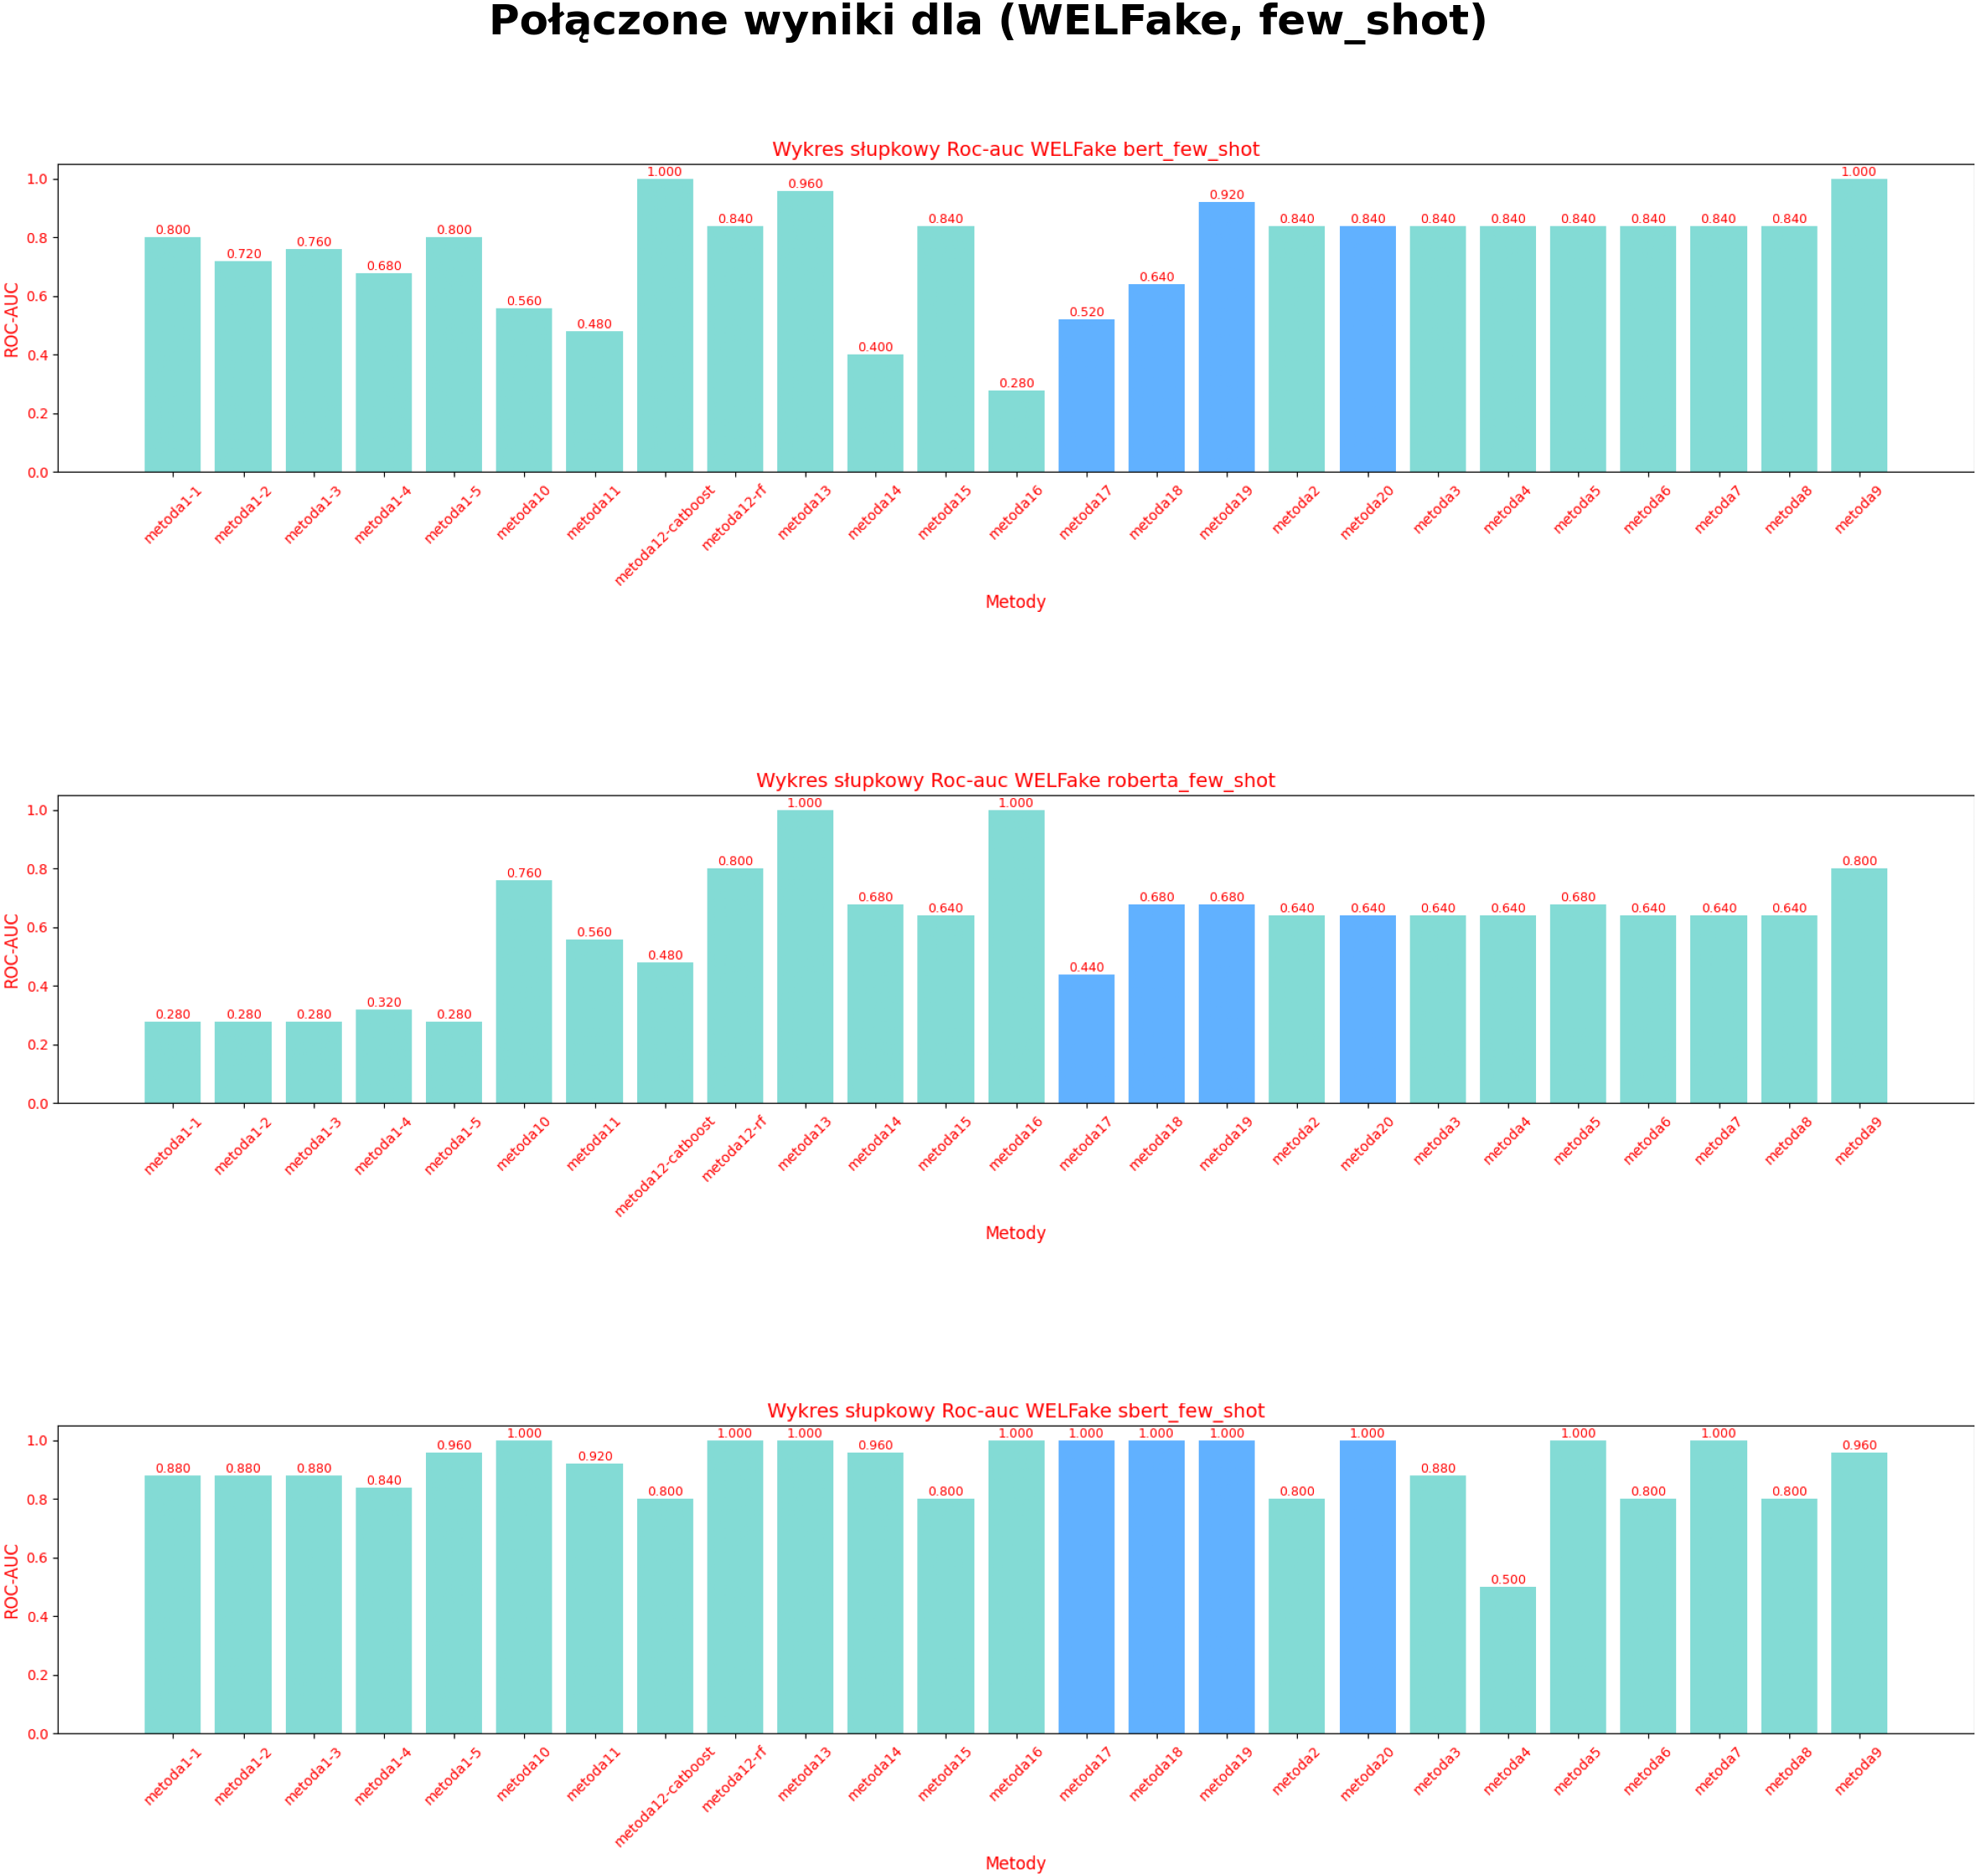
\includegraphics[width=0.99\textwidth]{img/stats/WELFake_few_shot/WELFake_few_shot_Combined_ROC-AUC_bar.png}
	\caption{Histogram rozkładu \textbf{Pola pod krzywą ROC-AUC (ROC-AUC)}.}
	\label{fig:welfake_few_shot_roc}
\end{figure}

\subsubsection{Czas wykonania}
Wykres liniowy \textbf{Czasu wykonania (Execution Time)} \ref{fig:welfake_few_shot_prcurve} przedstawia porównanie czasu potrzebnego na wykonanie predykcji. Na podstawie wykresów można sformułować następujące obserwacje:

\begin{itemize}
	\item \textbf{Wykres górny (BERT):}
	      \begin{itemize}
		      \item Najwięcej czasu, powyżej 500 sekund, zajęły \texttt{Metoda9} oraz \texttt{Metoda20}. \texttt{Metoda9} jest czasochłonna z powodu iteracyjnych algorytmów ensemble, a \texttt{Metoda20} z powodu trenowania LightGBM na dużych danych BERT.
		      \item Najkrótszy czas, poniżej 20 sekund, miały \texttt{Metoda18}, \texttt{Metoda7} oraz \texttt{Metoda10}, dzięki zoptymalizowanym modelom.
	      \end{itemize}

	\item \textbf{Wykres środkowy (RoBERTa):}
	      \begin{itemize}
		      \item Najwięcej czasu, od 200 do 500 sekund, zajęły \texttt{Metoda14}, \texttt{Metoda9} oraz \texttt{Metoda17}. \texttt{Metoda17} wymaga dodatkowego czasu na optymalizację VotingClassifiera.
		      \item Najkrótszy czas, poniżej 20 sekund, miały \texttt{Metoda18}, \texttt{Metoda7} oraz \texttt{Metoda10}.
	      \end{itemize}

	\item \textbf{Wykres dolny (SBERT):}
	      \begin{itemize}
		      \item Najdłuższy czas, około 2000 sekund, osiągnęła \texttt{Metoda4} z powodu złożonych warstw Bi-LSTM, CNN i MLP.
		      \item Najkrótszy czas, do 50 sekund, uzyskano dla \texttt{Metoda7} oraz \texttt{Metoda19}, dzięki prostym i zoptymalizowanym modelom.
	      \end{itemize}
\end{itemize}

Analiza czasów wykonania dla trybu few-shot pokazuje, że złożone modele, takie jak \texttt{Metoda4} czy \texttt{Metoda20}, są czasochłonne, podczas gdy \texttt{Metoda18} i \texttt{Metoda19} osiągają wysoką efektywność czasową, szczególnie dla SBERT.

\begin{figure}[H]
	\centering
	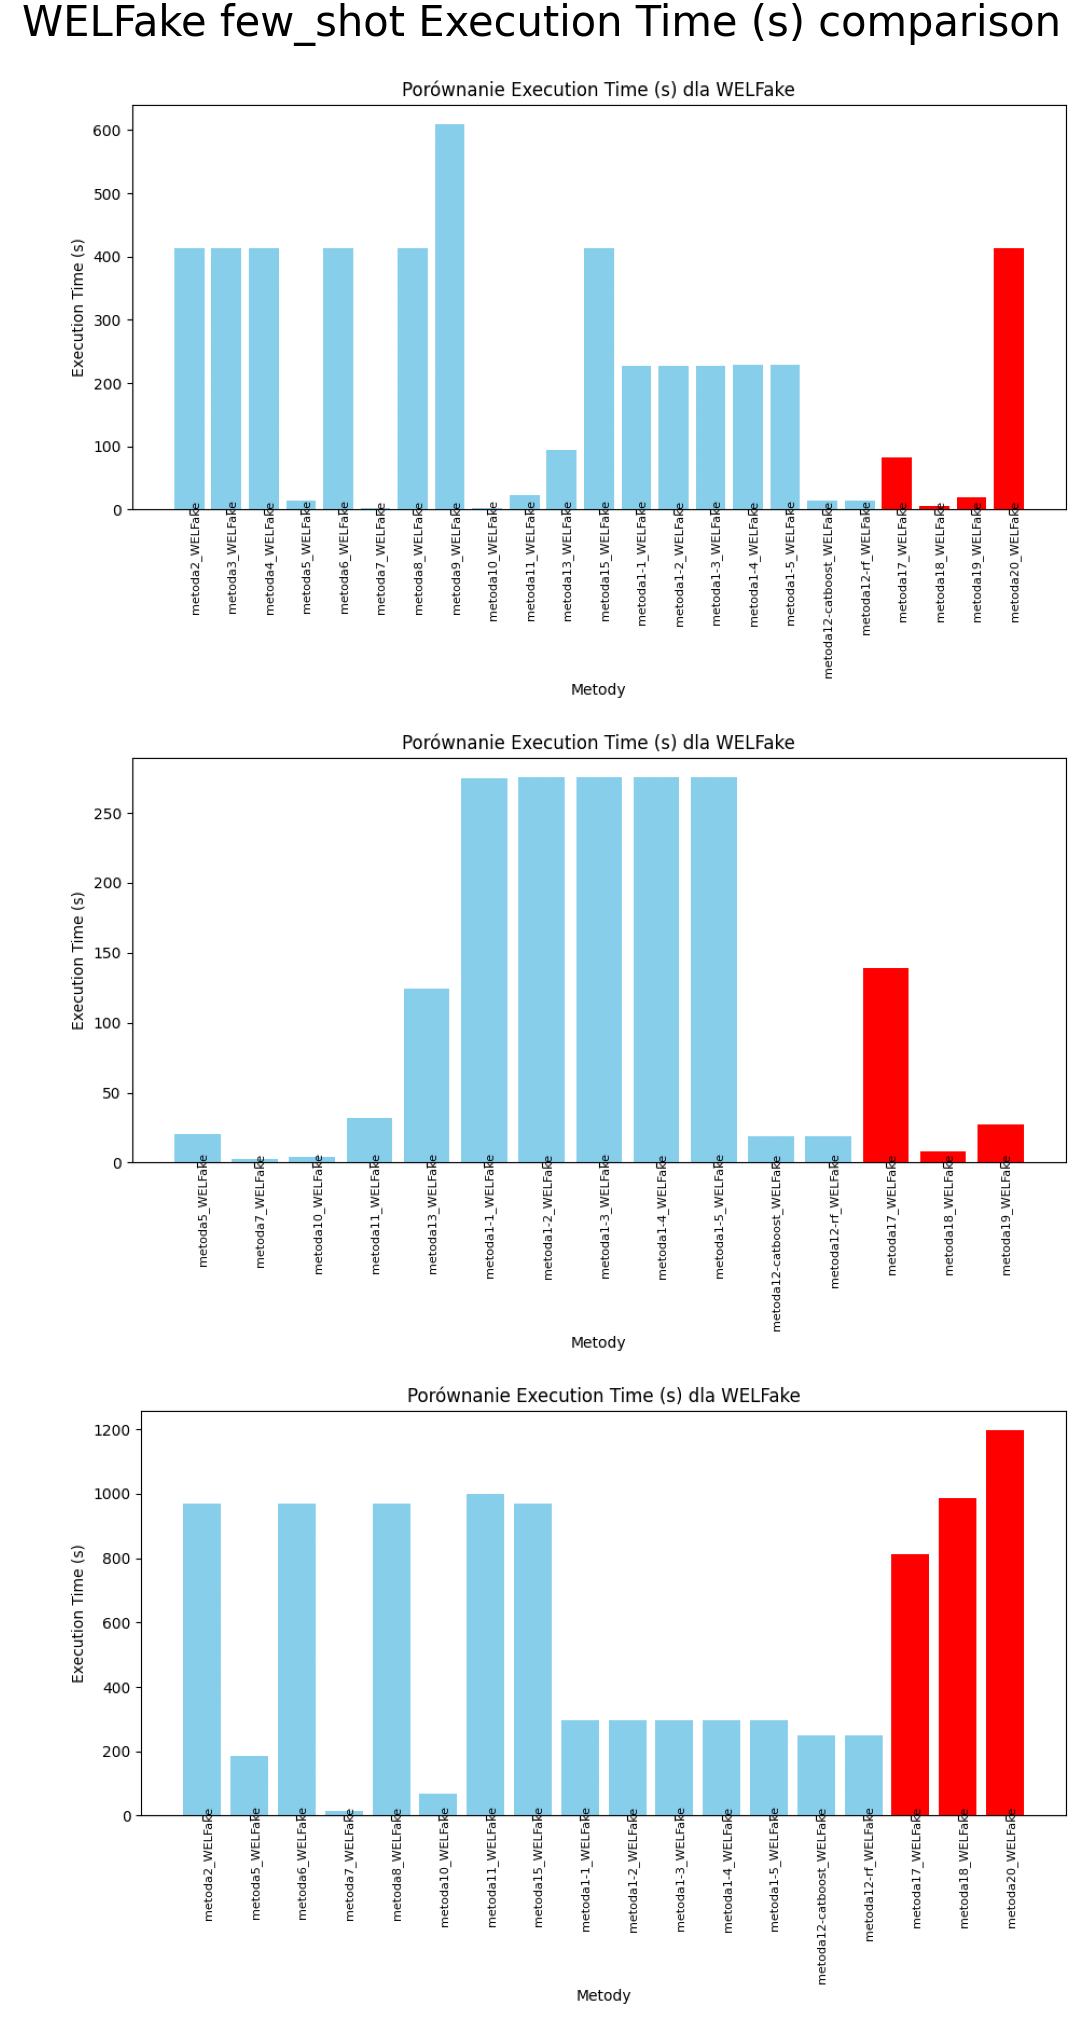
\includegraphics[width=0.99\textwidth]{img/stats/WELFake_few_shot/WELFake_few_shot_Execution Time (s)_comparison.png}
	\caption{\textbf{Czas wykonania (Execution Time)} w sekundach.}
	\label{fig:welfake_few_shot_prcurve}
\end{figure}

% Subsection for one-shot mode results
\subsection{Wyniki w trybie one-shot}

W trybie \textbf{one-shot} dla datasetu \textbf{WELFake} przetestowano metody klasyfikacji na pojedynczych przykładach treningowych. Poniżej przedstawiono szczegółowy opis wyników.

\subsubsection{Accuracy}
Wykresy słupkowe \textbf{Dokładności (Accuracy)} \ref{fig:welfake_one_shot_accuracy} przedstawiają rozkład wartości dokładności dla wszystkich metod. Na podstawie wykresów można sformułować następujące obserwacje:

\begin{itemize}
	\item \textbf{Wykres górny (BERT):}
	      \begin{itemize}
		      \item Większość metod osiągnęła dokładność około 1.0, co wskazuje na wysoką separowalność klas w danych BERT w trybie one-shot.
		      \item Najgorsze wyniki, około 0.5, odnotowano dla \texttt{Metoda17} oraz \texttt{Metoda11}. Słabe wyniki \texttt{Metoda17} mogą wynikać z nieoptymalnych wag VotingClassifiera.
	      \end{itemize}

	\item \textbf{Wykres środkowy (RoBERTa):}
	      \begin{itemize}
		      \item Wszystkie metody osiągnęły umiarkowaną dokładność, około 0.6, co wskazuje na trudności w generalizacji z pojedynczego przykładu dla RoBERTa.
		      \item Brak wyraźnych liderów sugeruje, że embeddingi RoBERTa są mniej separowalne w trybie one-shot.
	      \end{itemize}

	\item \textbf{Wykres dolny (SBERT):}
	      \begin{itemize}
		      \item Większość metod osiągnęła dokładność około 1.0, potwierdzając wysoką informatywność embeddingów SBERT.
		      \item Najgorsze wyniki, około 0.5, odnotowano dla \texttt{Metoda3}, \texttt{Metoda4}, \texttt{Metoda7}, \texttt{Metoda12-rf} oraz \texttt{Metoda19}. Słabe wyniki \texttt{Metoda19} mogą wynikać z braku optymalizacji ensemble.
	      \end{itemize}
\end{itemize}

Analiza dokładności dla trybu one-shot pokazuje, że BERT i SBERT umożliwiają perfekcyjne wyniki dla wielu metod, podczas gdy RoBERTa osiąga umiarkowane wyniki z powodu subtelniejszych reprezentacji.

\begin{figure}[H]
	\centering
	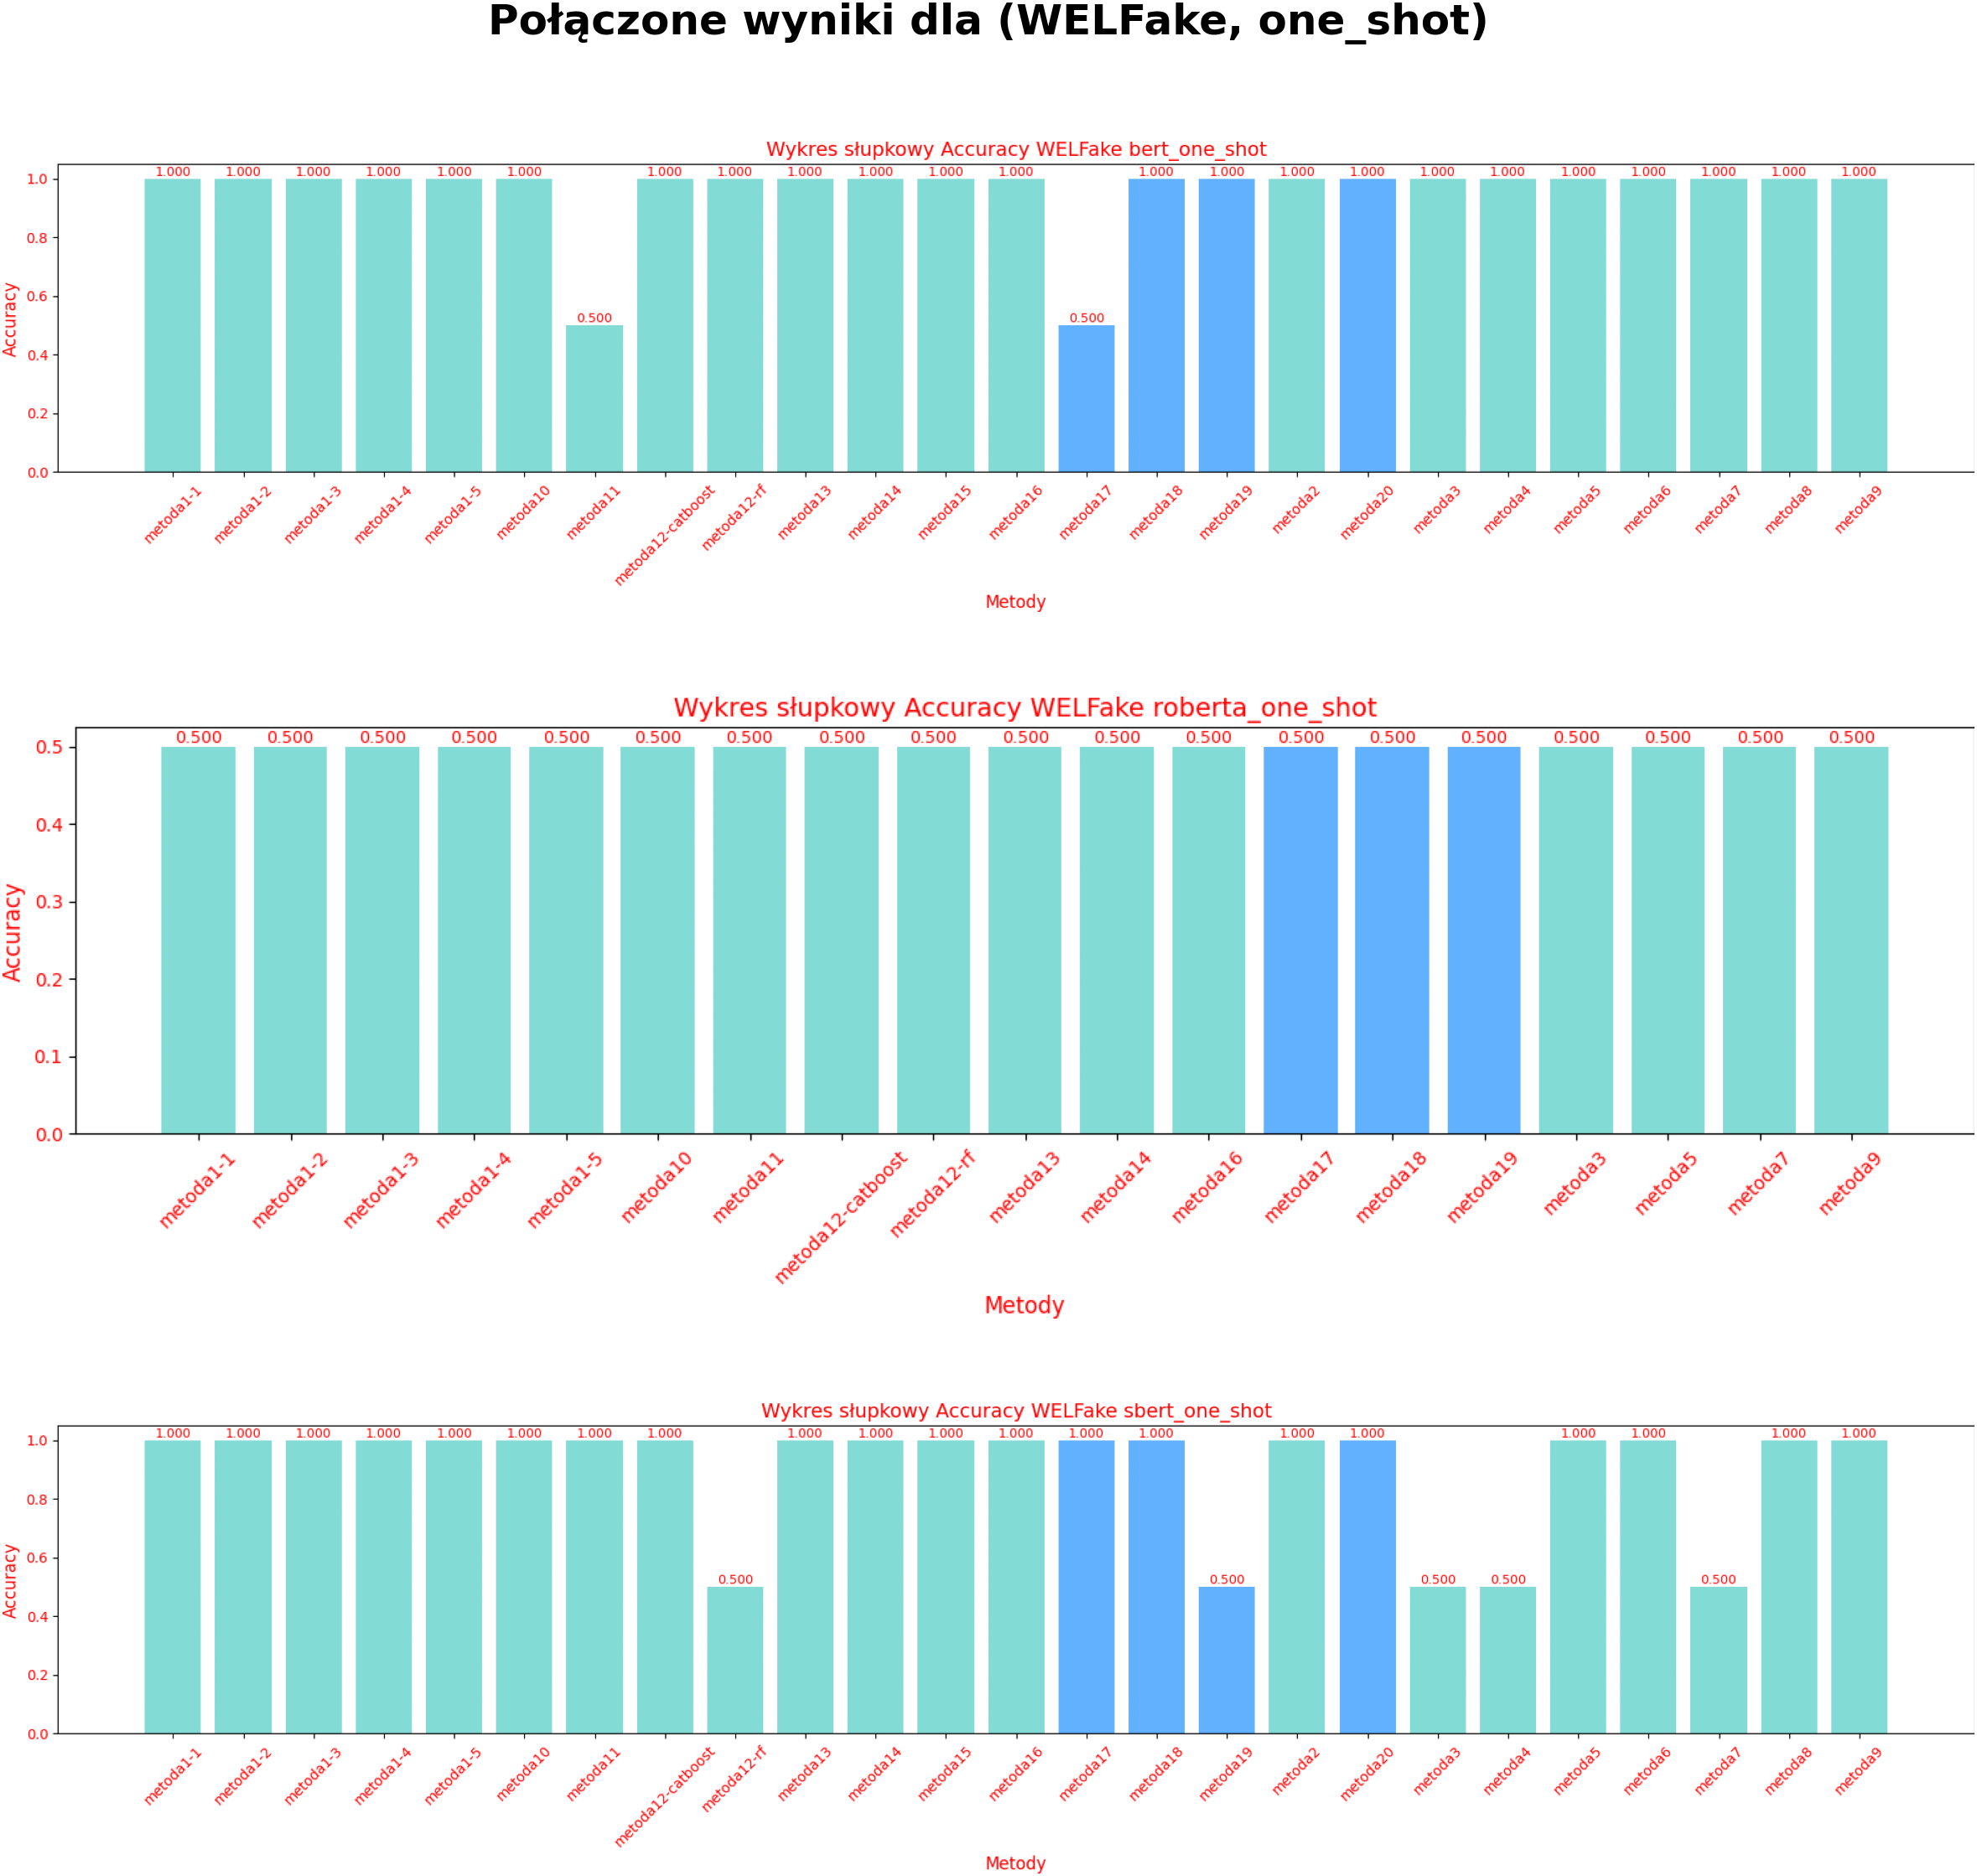
\includegraphics[width=0.99\textwidth]{img/stats/WELFake_one_shot/WELFake_one_shot_Combined_Accuracy_bar_chart.png}
	\caption{Histogram rozkładu \textbf{Dokładności (Accuracy)}.}
	\label{fig:welfake_one_shot_accuracy}
\end{figure}

\subsubsection{F1-Score}
Wykresy słupkowe \textbf{Wyniku F1 (F1-Score)} \ref{fig:welfake_one_shot_f1} przedstawiają rozkład wartości F1-Score dla wszystkich metod. Na podstawie wykresu można sformułować następujące obserwacje:

\begin{itemize}
	\item \textbf{Wykres górny (BERT):}
	      \begin{itemize}
		      \item Większość metod osiągnęła F1-Score około 1.0, co potwierdza wysoką separowalność klas w danych BERT.
		      \item Najniższe wyniki, około 0.5, odnotowano dla \texttt{Metoda17} oraz \texttt{Metoda11}. Słabe wyniki \texttt{Metoda17} mogą wynikać z niedopasowania VotingClassifiera.
	      \end{itemize}

	\item \textbf{Wykres środkowy (RoBERTa):}
	      \begin{itemize}
		      \item Większość metod osiągnęła F1-Score około 0.7, co wskazuje na trudności w trybie one-shot dla RoBERTa.
		      \item Najsłabsze wyniki, około 0.5, odnotowano dla \texttt{Metoda1-5}, \texttt{Metoda13} oraz \texttt{Metoda19}. Słabe wyniki \texttt{Metoda19} mogą wynikać z braku optymalizacji.
	      \end{itemize}

	\item \textbf{Wykres dolny (SBERT):}
	      \begin{itemize}
		      \item Większość metod osiągnęła F1-Score około 1.0, potwierdzając informatywność SBERT.
		      \item Najgorsze rezultaty, około 0.5, odnotowano dla \texttt{Metoda3}, \texttt{Metoda4}, \texttt{Metoda7}, \texttt{Metoda12-rf} oraz \texttt{Metoda19}. Słabe wyniki \texttt{Metoda19} wskazują na potrzebę lepszej optymalizacji.
	      \end{itemize}
\end{itemize}

Analiza F1-Score dla trybu one-shot potwierdza wysoką skuteczność BERT i SBERT, podczas gdy RoBERTa wymaga precyzyjniejszej optymalizacji.

\begin{figure}[H]
	\centering
	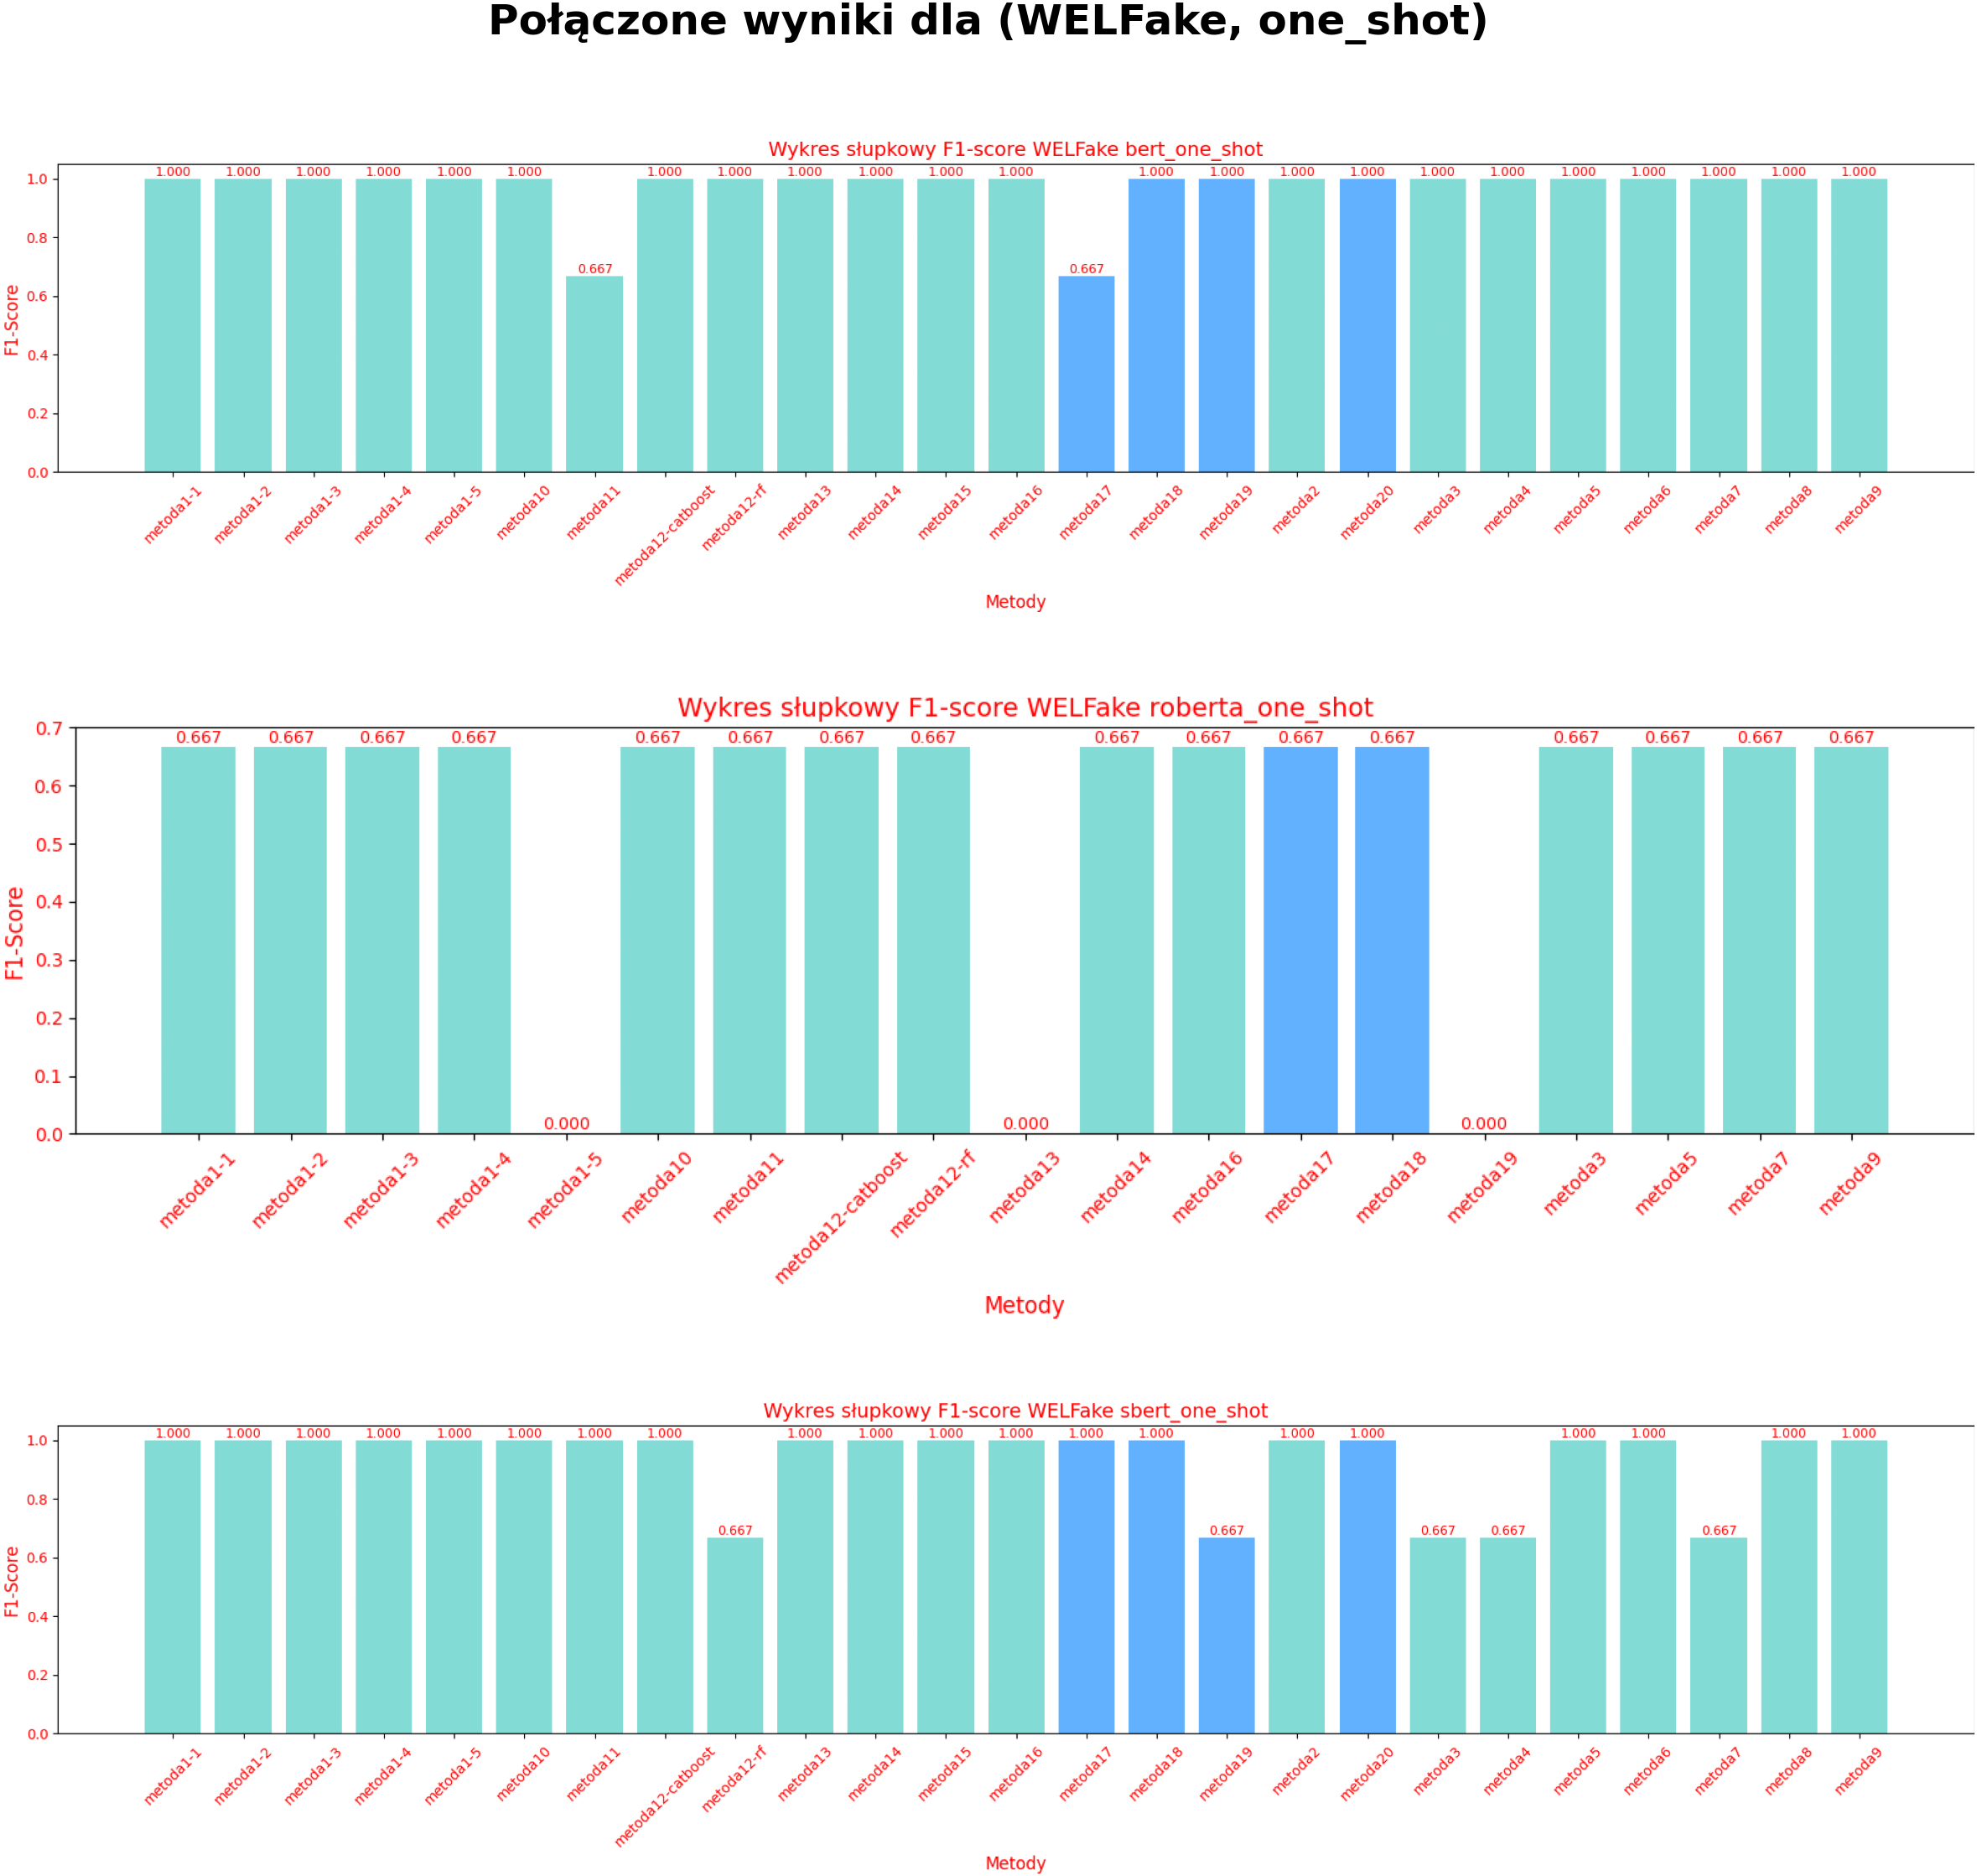
\includegraphics[width=0.99\textwidth]{img/stats/WELFake_one_shot/WELFake_one_shot_Combined_F1-Score_bar.png}
	\caption{Histogram rozkładu \textbf{Wyniku F1 (F1-Score)}.}
	\label{fig:welfake_one_shot_f1}
\end{figure}

\subsubsection{ROC-AUC}
Wykresy słupkowe \textbf{Pola pod krzywą ROC-AUC (ROC-AUC)} \ref{fig:welfake_one_shot_roc} przedstawiają rozkład wartości ROC-AUC dla wszystkich metod. Na podstawie wykresu można sformułować następujące obserwacje:

\begin{itemize}
	\item \textbf{Wykres górny (BERT):}
	      \begin{itemize}
		      \item Wszystkie metody osiągnęły ROC-AUC około 1.0, co potwierdza doskonałą separowalność klas w danych BERT.
	      \end{itemize}

	\item \textbf{Wykres środkowy (RoBERTa):}
	      \begin{itemize}
		      \item Najlepsze wartości ROC-AUC, około 0.9, osiągnęły \texttt{Metoda12-rf}, \texttt{Metoda13}, \texttt{Metoda17} oraz \texttt{Metoda18}. Wysoka skuteczność wskazuje na zdolność tych metod do rozróżniania klas.
		      \item Najsłabsze wyniki, około 0.6, odnotowano dla pozostałych metod, w tym \texttt{Metoda19}. Słabe wyniki \texttt{Metoda19} mogą wynikać z braku optymalizacji.
	      \end{itemize}

	\item \textbf{Wykres dolny (SBERT):}
	      \begin{itemize}
		      \item Większość metod osiągnęła ROC-AUC około 1.0, potwierdzając informatywność SBERT.
		      \item Słabe rezultaty, około 0.5, odnotowano dla \texttt{Metoda4}. Niska wartość ROC-AUC może wynikać z trudności w optymalizacji złożonej architektury.
	      \end{itemize}
\end{itemize}

Analiza ROC-AUC dla trybu one-shot pokazuje, że BERT i SBERT umożliwiają perfekcyjne wyniki, podczas gdy RoBERTa wymaga lepszej optymalizacji dla niektórych metod, takich jak \texttt{Metoda19}.

\begin{figure}[H]
	\centering
	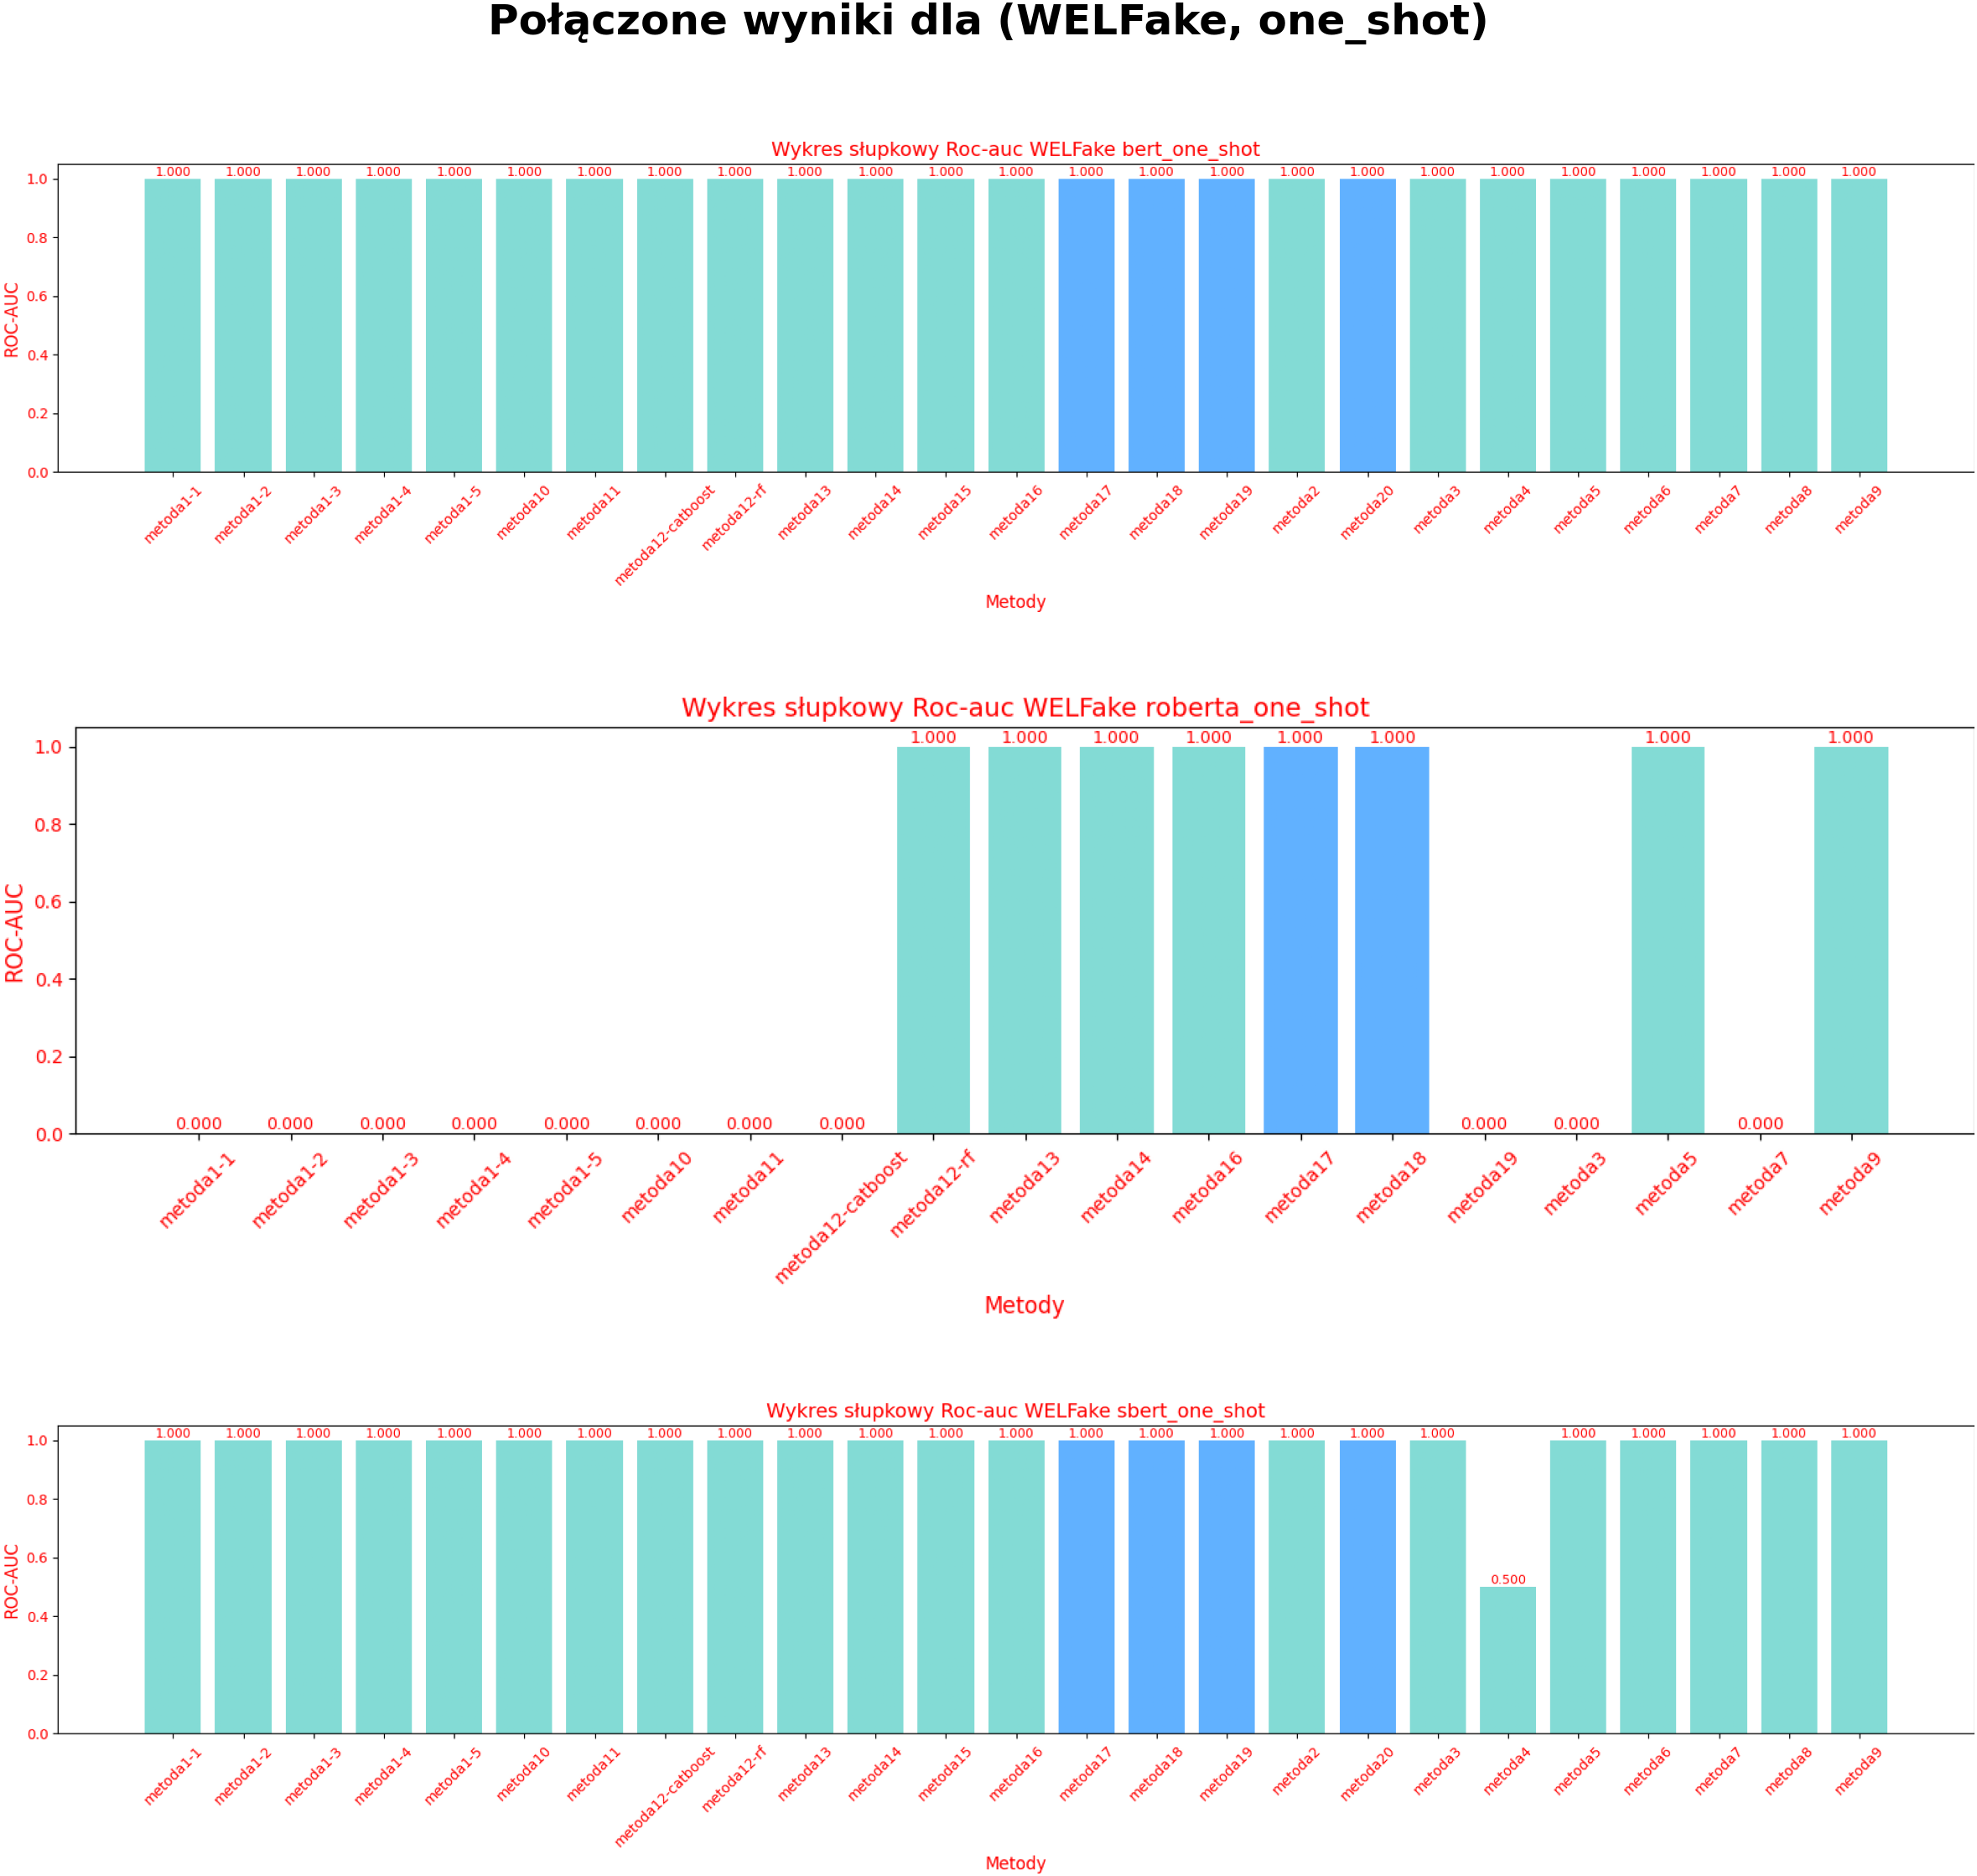
\includegraphics[width=0.99\textwidth]{img/stats/WELFake_one_shot/WELFake_one_shot_Combined_ROC-AUC_bar.png}
	\caption{Histogram rozkładu \textbf{Pola pod krzywą ROC-AUC (ROC-AUC)}.}
	\label{fig:welfake_one_shot_roc}
\end{figure}

\subsubsection{Czas wykonania}
Wykres liniowy \textbf{Czasu wykonania (Execution Time)} \ref{fig:welfake_one_shot_prcurve} przedstawia porównanie czasu potrzebnego na wykonanie predykcji. Na podstawie wykresów można sformułować następujące obserwacje:

\begin{itemize}
	\item \textbf{Wykres górny (BERT):}
	      \begin{itemize}
		      \item Najdłuższy czas, około 140 sekund, odnotowano dla \texttt{Metoda2}, \texttt{Metoda3}, \texttt{Metoda4}, \texttt{Metoda8}, \texttt{Metoda15} oraz \texttt{Metoda20}. \texttt{Metoda20} jest czasochłonna z powodu trenowania LightGBM na dużych danych.
		      \item Najkrótszy czas, poniżej 10 sekund, miały \texttt{Metoda7}, \texttt{Metoda10} oraz \texttt{Metoda18}.
	      \end{itemize}

	\item \textbf{Wykres środkowy (RoBERTa):}
	      \begin{itemize}
		      \item Najwięcej czasu, około 400 sekund, zajęła \texttt{Metoda9} z powodu iteracyjnych algorytmów ensemble.
		      \item Najkrótszy czas, poniżej 5 sekund, miały \texttt{Metoda7}, \texttt{Metoda18} oraz \texttt{Metoda19}.
	      \end{itemize}

	\item \textbf{Wykres dolny (SBERT):}
	      \begin{itemize}
		      \item Najdłuższy czas, przekraczający 1200 sekund, osiągnęła \texttt{Metoda3} z powodu złożonej architektury ensemble.
		      \item Najkrótszy czas, w okolicach 100 sekund, uzyskano dla \texttt{Metoda7}, \texttt{Metoda17} oraz \texttt{Metoda19}.
	      \end{itemize}
\end{itemize}

Analiza czasów wykonania dla trybu one-shot pokazuje, że złożone modele, takie jak \texttt{Metoda3} czy \texttt{Metoda20}, są czasochłonne, podczas gdy \texttt{Metoda18} i \texttt{Metoda19} osiągają wysoką efektywność czasową.

\begin{figure}[H]
	\centering
	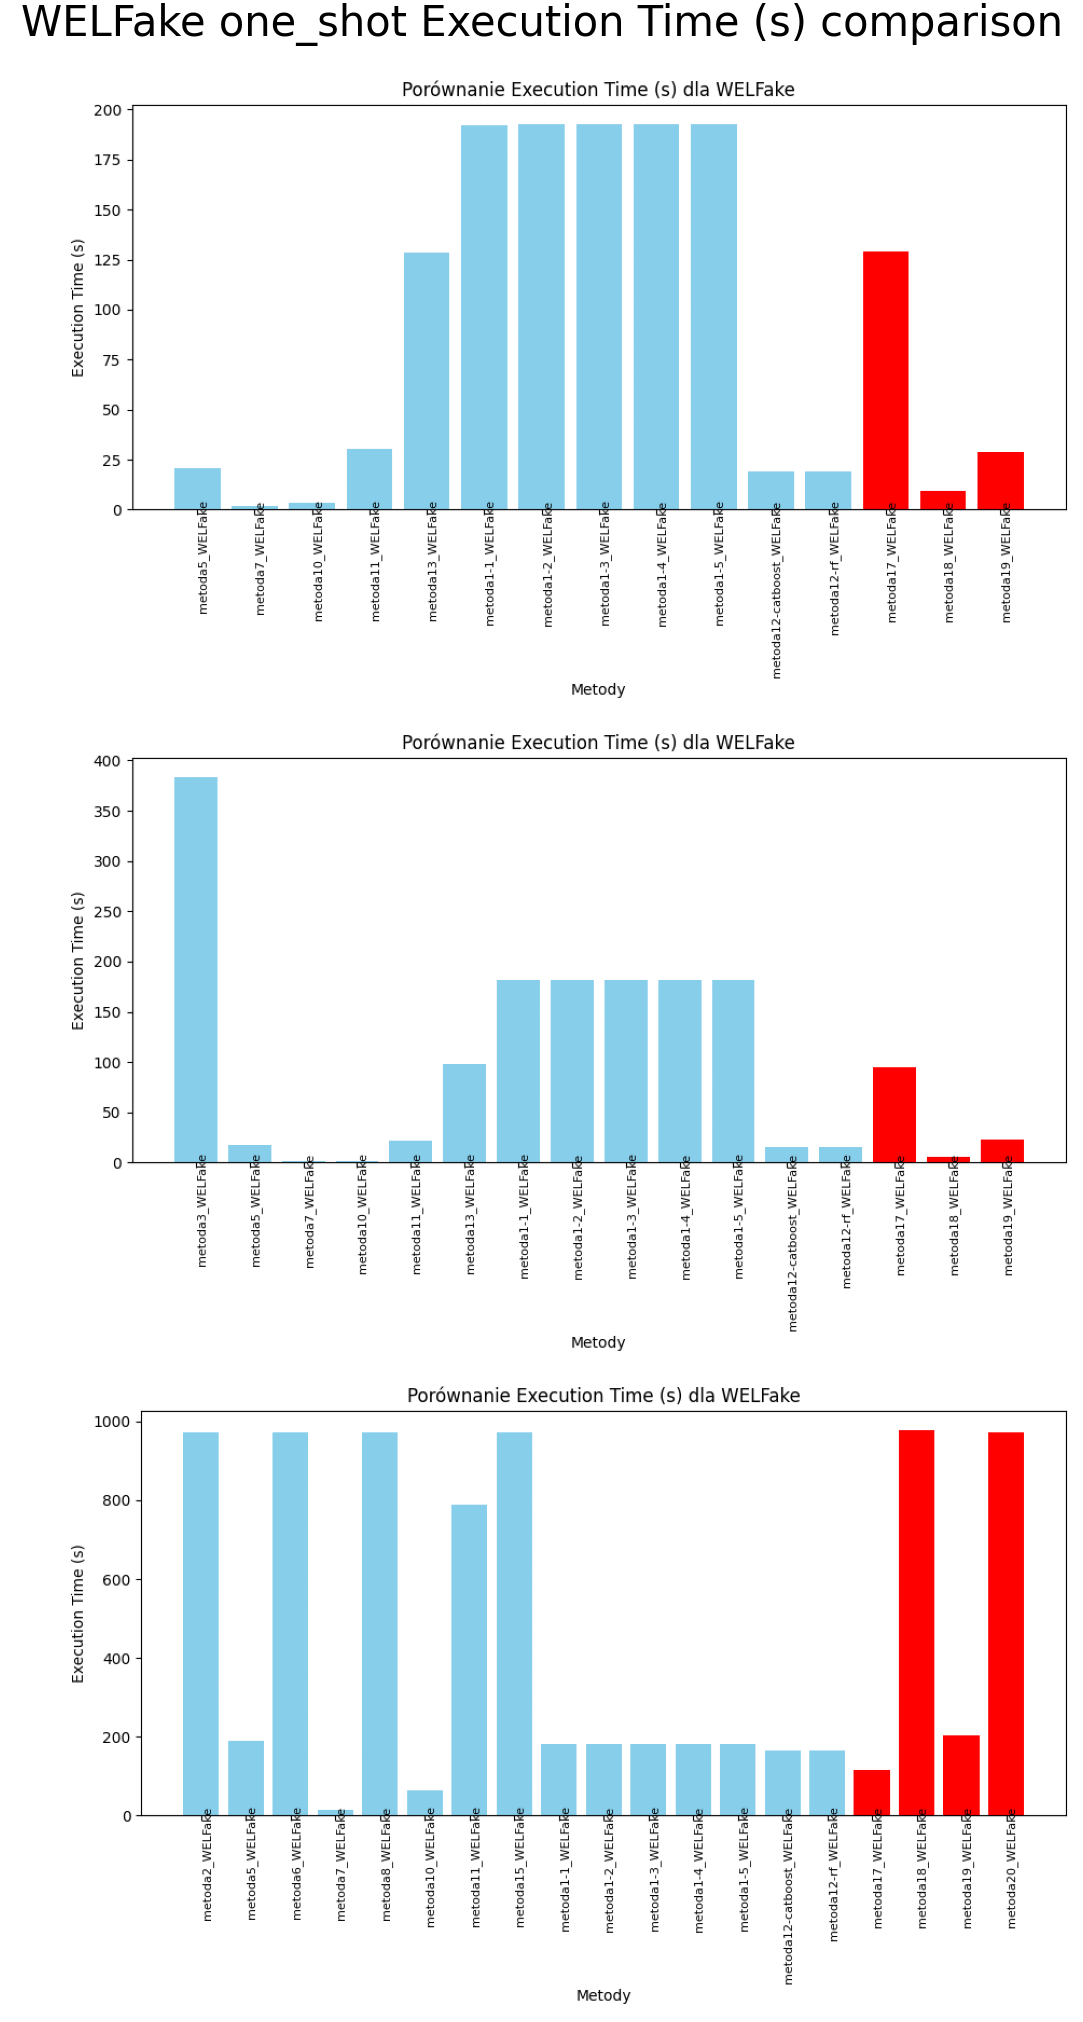
\includegraphics[width=0.99\textwidth]{img/stats/WELFake_one_shot/WELFake_one_shot_Execution Time (s)_comparison.png}
	\caption{\textbf{Czas wykonania (Execution Time)} w sekundach.}
	\label{fig:welfake_one_shot_prcurve}
\end{figure}

% Subsection for additional analysis
\subsection{Dodatkowa analiza wyników dla datasetu WELFake}
\label{subsec:welfake_additional_analysis}

W tej podsekcji przedstawiono szczegółową analizę wyników dla datasetu \textbf{WELFake}, obejmującą wyniki AUC-PR, testy normalności rozkładów, macierze korelacji Pearsona i Spearmana oraz testy statystyczne Kruskal-Wallis. Analiza ma na celu ocenę wydajności wszystkich metod oraz uzasadnienie sensu stosowania bardziej złożonych metod autorskich (\texttt{Metoda17}, \texttt{Metoda18}, \texttt{Metoda19}, \texttt{Metoda20}) w kontekście ich zalet w różnych scenariuszach uczenia.

\subsubsection{Wyniki AUC-PR}
Tabela \ref{tab:welfake_auc_pr} przedstawia wyniki AUC-PR dla różnych metod. Najwyższy wynik, 0.9556, osiągnęła \texttt{Metoda13}. Wśród metod autorskich \texttt{Metoda18} osiągnęła 0.8932, \texttt{Metoda20} 0.8863, \texttt{Metoda17} 0.8469, a \texttt{Metoda19} 0.8266. \texttt{Metoda17} osiąga średnie wyniki z powodu nieoptymalnych wag VotingClassifiera. \texttt{Metoda18} jest skuteczna dzięki stackingowi z CatBoost. \texttt{Metoda19} ma słabsze wyniki z powodu braku balansowania klas. \texttt{Metoda20} osiąga dobre wyniki dzięki zoptymalizowanemu LightGBM.

\begin{table}[H]
	\centering
	\caption{Wyniki AUC-PR dla metod na datasecie WELFake}
	\label{tab:welfake_auc_pr}
	\begin{tabular}{l r}
		\toprule
		Metoda                     & AUC-PR \\
		\midrule
		\texttt{metoda13}          & 0.9556 \\
		\texttt{metoda12-rf}       & 0.9248 \\
		\texttt{metoda9}           & 0.9207 \\
		\texttt{metoda5}           & 0.8982 \\
		\texttt{metoda14}          & 0.8955 \\
		\texttt{metoda18}          & 0.8932 \\
		\texttt{metoda16}          & 0.8923 \\
		\texttt{metoda20}          & 0.8863 \\
		\texttt{metoda2}           & 0.8633 \\
		\texttt{metoda8}           & 0.8633 \\
		\texttt{metoda15}          & 0.8633 \\
		\texttt{metoda6}           & 0.8633 \\
		\texttt{metoda17}          & 0.8469 \\
		\texttt{metoda19}          & 0.8266 \\
		\texttt{metoda10}          & 0.8126 \\
		\texttt{metoda7}           & 0.8111 \\
		\texttt{metoda12-catboost} & 0.8109 \\
		\texttt{metoda4}           & 0.8054 \\
		\texttt{metoda3}           & 0.7989 \\
		\texttt{metoda11}          & 0.7912 \\
		\texttt{metoda1-5}         & 0.7730 \\
		\texttt{metoda1-1}         & 0.7623 \\
		\texttt{metoda1-3}         & 0.7579 \\
		\texttt{metoda1-2}         & 0.7575 \\
		\texttt{metoda1-4}         & 0.7527 \\
		\bottomrule
	\end{tabular}
\end{table}

\subsubsection{Testy normalności i analizy statystyczne}
Testy Shapiro-Wilka wykazały, że większość metryk (Accuracy, Precision, Recall, F1-Score, ROC-AUC, MCC, Cohen’s Kappa, AUC-PR) ma rozkład normalny (p-value > 0.05), z wyjątkiem Accuracy dla \texttt{Metoda17} (p-value = 0.0065). Testy Kruskal-Wallisa nie wykazały istotnych statystycznych różnic między metodami (p-value > 0.05), z najwyższym p-value dla F1-Score (0.9669). Wynik ten sugeruje, że prostsze metody, takie jak \texttt{Metoda9}, mogą być równie skuteczne jak bardziej złożone metody autorskie w trybie klasycznym, ale złożone metody oferują przewagę w trudniejszych scenariuszach, takich jak few-shot i one-shot.

\subsubsection{Analiza korelacji}
Macierze korelacji Pearsona i Spearmana ujawniły silne dodatnie zależności między metrykami. Najsilniejsze korelacje w macierzy Pearsona zaobserwowano między Accuracy a Cohen’s Kappa (0.9990), Accuracy a MCC (0.9972) oraz ROC-AUC a AUC-PR (0.9689). W macierzy Spearmana korelacje te wynoszą odpowiednio 0.9900, 0.9815 oraz 0.9691. Brak silnych ujemnych korelacji wskazuje na zgodność metryk w ocenie wydajności modeli.

\begin{table}[H]
	\centering
	\caption{Kluczowe współczynniki korelacji Pearsona}
	\label{tab:welfake_pearson_correlations}
	\begin{tabular}{l r l}
		\toprule
		Para metryk               & Współczynnik Pearsona & Interpretacja         \\
		\midrule
		Accuracy -- Cohen’s Kappa & 0.9990                & Bardzo silna dodatnia \\
		Accuracy -- MCC           & 0.9972                & Bardzo silna dodatnia \\
		MCC -- Cohen’s Kappa      & 0.9969                & Bardzo silna dodatnia \\
		Precision -- F1-Score     & 0.7951                & Silna dodatnia        \\
		Recall -- F1-Score        & 0.5878                & Umiarkowana dodatnia  \\
		ROC-AUC -- AUC-PR         & 0.9689                & Bardzo silna dodatnia \\
		\bottomrule
	\end{tabular}
\end{table}

\begin{table}[H]
	\centering
	\caption{Kluczowe współczynniki korelacji Spearmana}
	\label{tab:welfake_spearman_correlations}
	\begin{tabular}{l r l}
		\toprule
		Para metryk               & Współczynnik Spearmana & Interpretacja         \\
		\midrule
		Accuracy -- Cohen’s Kappa & 0.9900                 & Bardzo silna dodatnia \\
		Accuracy -- MCC           & 0.9815                 & Bardzo silna dodatnia \\
		MCC -- Cohen’s Kappa      & 0.9707                 & Bardzo silna dodatnia \\
		Precision -- F1-Score     & 0.6672                 & Silna dodatnia        \\
		Recall -- F1-Score        & 0.5145                 & Umiarkowana dodatnia  \\
		ROC-AUC -- AUC-PR         & 0.9691                 & Bardzo silna dodatnia \\
		\bottomrule
	\end{tabular}
\end{table}

% Subsection for conclusions
\subsection{Podsumowanie wniosków}
Analiza wyników dla datasetu \textbf{WELFake} pokazuje, że zaawansowane modele ensemble, takie jak \texttt{Metoda12-rf}, \texttt{Metoda13}, \texttt{Metoda18} oraz \texttt{Metoda19}, osiągają wysoką skuteczność w trybach klasycznym, few-shot i one-shot, szczególnie dla embeddingów \textbf{SBERT}. W trybie one-shot \textbf{BERT} i \textbf{SBERT} umożliwiają perfekcyjne wyniki (około 100\% Accuracy i F1-Score) dla wielu metod, co świadczy o ich zdolności do generowania wysoce separowalnych reprezentacji. \textbf{RoBERTa} osiąga umiarkowane wyniki (60–70\%) w trybie one-shot z powodu subtelniejszych reprezentacji, które wymagają precyzyjniejszej optymalizacji.

\begin{itemize}
	\item \textbf{Metoda17} (VotingClassifier) jest skuteczna dla \textbf{SBERT} w trybach klasycznym i few-shot dzięki elastyczności VotingClassifiera, ale słaba dla \textbf{BERT} i \textbf{RoBERTa} z powodu nieoptymalnych wag głosowania, co ogranicza jej zdolność do generalizacji.
	\item \textbf{Metoda18} (stacking z CatBoost) dominuje dla \textbf{SBERT} w trybach klasycznym i few-shot dzięki zoptymalizowanemu łączeniu modeli bazowych, ale osiąga słabsze wyniki dla \textbf{RoBERTa} w trybie one-shot z powodu zbyt prostej konfiguracji meta-klasyfikatora.
	\item \textbf{Metoda19} (stacking) osiąga wysokie wyniki dla \textbf{BERT} i \textbf{RoBERTa} w trybach klasycznym i few-shot dzięki zoptymalizowanemu ensemble, ale jest słaba dla \textbf{SBERT} w trybie one-shot z powodu braku odpowiedniego balansowania klas.
	\item \textbf{Metoda20} (LightGBM) jest skuteczna dla \textbf{BERT} i \textbf{SBERT} w trybie one-shot dzięki zoptymalizowanym modelom, ale osiąga średnie wyniki w innych trybach z powodu braku balansowania klas.
	\item Prostsze modele, takie jak \texttt{Metoda1-x}, osiągają zróżnicowane wyniki, z dobrymi rezultatami dla \textbf{SBERT}, ale słabszymi dla \textbf{RoBERTa}, co wskazuje na ich ograniczenia w trudniejszych scenariuszach.
\end{itemize}

Wysoka separowalność klas w datasecie \textbf{WELFake} ułatwia klasyfikację dla zoptymalizowanych metod, takich jak \texttt{Metoda18} i \texttt{Metoda19}, ale wymaga precyzyjnej konfiguracji hiperparametrów w trudniejszych scenariuszach, takich jak tryb one-shot dla \textbf{RoBERTa}. Sens stosowania bardziej złożonych metod autorskich jest uzasadniony ich stabilnością i elastycznością w trudniejszych scenariuszach, co czyni je atrakcyjnymi w praktycznych zastosowaniach wymagających uniwersalności i wysokiej jakości predykcji.